% Classe default, de acordo com o modelo:
\documentclass[11pt,a4paper,openright,titlepage,oneside]{book}

% Classe alternativa, apropriada para impressão frente-verso. Inclui páginas em branco
% de forma que capítulos sempre tenham início na página à direita:
% \documentclass[11pt,a4paper,openright,titlepage]{book}

% Pacotes

\usepackage{epsfig}
\usepackage{epsf}
\usepackage{epstopdf}
\usepackage{pst-eps}
\usepackage{graphicx}
\usepackage{graphics}
%\usepackage[table,xcdraw]{xcolor}
\usepackage{tabu}
\usepackage{booktabs}
\usepackage{tabularx}
\usepackage{caption}
\usepackage{booktabs}
\usepackage{longtable}
\usepackage[T1]{fontenc}
\usepackage[brazilian, portuguese]{babel}
\usepackage{epsfig}
\usepackage{verbatim}
\usepackage{epstopdf}
\usepackage{subfigure}
\usepackage{amsfonts}
\usepackage{amsmath}
\usepackage{amssymb}
\usepackage[thmmarks,amsmath]{ntheorem}%\usepackage{amsthm}
\usepackage{boxedminipage}
\usepackage{geometry}
\usepackage{theorem}
\usepackage{fancybox}
\usepackage{fancyhdr}
\usepackage{ifthen}
\usepackage{url}
\usepackage{afterpage}
\usepackage{color}
\usepackage{colortbl}
\usepackage{rotating}
\usepackage{makeidx}
\usepackage{indentfirst}
\usepackage{epstopdf}
\usepackage{listingsutf8}
\usepackage{float}
\usepackage{listings}
\usepackage{color}

\usepackage{typearea}
\usepackage{listings}
\renewcommand{\lstlistingname}{Code}
\captionsetup[lstlisting]{font={small,tt}} 
%%%%Umlaute äöü für dieses Paket definieren
\lstset{basicstyle=\ttfamily}
\lstset{literate=%
	{Ö}{{\"O}}1
	{Ä}{{\"A}}1
	{Ü}{{\"U}}1
	{ß}{{\ss}}2
	{ü}{{\"u}}1
	{ä}{{\"a}}1
	{ö}{{\"o}}1
}
%%%%%%%%%%%%%%%%%%%%%%%%%%%%%%%%%%%%%%%%%%%%   
\usepackage{etoolbox}    

\definecolor{mygreen}{rgb}{0,0.6,0}
\definecolor{mygray}{rgb}{0.47,0.47,0.33}
\definecolor{myorange}{rgb}{0.8,0.4,0}
\definecolor{mywhite}{rgb}{0.98,0.98,0.98}
\definecolor{myblue}{rgb}{0.01,0.61,0.98}

\newcommand*{\FormatDigit}[1]{\ttfamily\textcolor{mygreen}{#1}}
%% http://tex.stackexchange.com/questions/32174/listings-package-how-can-i-format-all-numbers
\lstdefinestyle{FormattedNumber}{%
	literate=*{0}{{\FormatDigit{0}}}{1}%
	{1}{{\FormatDigit{1}}}{1}%
	{2}{{\FormatDigit{2}}}{1}%
	{3}{{\FormatDigit{3}}}{1}%
	{4}{{\FormatDigit{4}}}{1}%
	{5}{{\FormatDigit{5}}}{1}%
	{6}{{\FormatDigit{6}}}{1}%
	{7}{{\FormatDigit{7}}}{1}%
	{8}{{\FormatDigit{8}}}{1}%
	{9}{{\FormatDigit{9}}}{1}%
	{.0}{{\FormatDigit{.0}}}{2}% Following is to ensure that only periods
	{.1}{{\FormatDigit{.1}}}{2}% followed by a digit are changed.
	{.2}{{\FormatDigit{.2}}}{2}%
	{.3}{{\FormatDigit{.3}}}{2}%
	{.4}{{\FormatDigit{.4}}}{2}%
	{.5}{{\FormatDigit{.5}}}{2}%
	{.6}{{\FormatDigit{.6}}}{2}%
	{.7}{{\FormatDigit{.7}}}{2}%
	{.8}{{\FormatDigit{.8}}}{2}%
	{.9}{{\FormatDigit{.9}}}{2}%
	%{,}{{\FormatDigit{,}}{1}% depends if you want the "," in color
	{\ }{{ }}{1}% handle the space
	,%
}


\lstset{%
	backgroundcolor=\color{mywhite},   
	basicstyle=\footnotesize,       
	breakatwhitespace=false,         
	breaklines=true,                 
	captionpos=b,                   
	commentstyle=\color{red},    
	deletekeywords={...},           
	escapeinside={\%*}{*)},          
	extendedchars=true,              
	%frame=shadowbox,                    
	keepspaces=true,                 
	keywordstyle=\color{myorange},       
	language=C,                
	morekeywords={*,...},            
	numbers=left,                    
	numbersep=5pt,                   
	numberstyle=\bfseries\tiny\color{mygray}, 
	rulecolor=\color{black},         
	%rulesepcolor=\color{myblue},
	showspaces=false,                
	showstringspaces=false,          
	showtabs=false,                  
	stepnumber=1,                    
	stringstyle=\color{myorange},    
	tabsize=2,                       
	title=\lstname,
	emphstyle=\bfseries\color{blue},%  style for emph={} 
}    

%% language specific settings:
\lstdefinestyle{Arduino}{%
	style=FormattedNumber,
	keywords={void},%                 define keywords
	morecomment=[l]{//},%             treat // as comments
	morecomment=[s]{/*}{*/},%         define /* ... */ comments
	emph={HIGH, OUTPUT, LOW},%        keywords to emphasize
}

\newtoggle{InString}{}% Keep track of if we are within a string
\togglefalse{InString}%


% Escolher um dos seguintes formatos:
%\usepackage{ft1unb} % segue padrão de fonte Times
\usepackage{ft2unb} % segue padrão de fontes do Latex

\makeindex
 
%%%%%%%%%%%%%%%%%%%%%%%%%%%%%%%%%%%%%%%%%%%%%%%%%%%%%%%%%%%%%%%%%%%%%%%%%
% Compilações parciais: com o comando abaixo, selecione apenas os capitulos
% que deseja compilar. Por exemplo, veja o que acontece se descomentar a
% linha abaixo:
%\includeonly{resumos,cap_Experimentos}
%%%%%%%%%%%%%%%%%%%%%%%%%%%%%%%%%%%%%%%%%%%%%%%%%%%%%%%%%%%%%%%%%%%%%%%%%

%%%%%%%%%%%%%%%%%%%%%%%%%%%%%%%%%%%%%%%%%%%%%%%%%%%%%%%%%%%%%%%%%%%%%%%%%
% Documento principal
%%%%%%%%%%%%%%%%%%%%%%%%%%%%%%%%%%%%%%%%%%%%%%%%%%%%%%%%%%%%%%%%%%%%%%%%%
\begin{document}

\setcounter{secnumdepth}{3} % numeração de seções até nível 3
\setcounter{tocdepth}{2} % numeração de seções no sumário até nível 2
\pagestyle{empty}

%%%%%%%%%%%%%%%%%%%%%%%%%%%%%%%%%%%%%%%%%%%%%%%%%%%%%%%%%%%%%%%%%%%%%%%%%
% Capa e contra-capa
%%%%%%%%%%%%%%%%%%%%%%%%%%%%%%%%%%%%%%%%%%%%%%%%%%%%%%%%%%%%%%%%%%%%%%%%%
% Grau pretendido e o tipo de monografia. Alguns exemplos seguem abaixo. Se o seu for algum deles, descomente-o. Em geral, o grau e o tipo de monografia associado estão na mesma linha.
%\grau{Doutor em Engenharia Elétrica} \tipodemonografia{TESE DE DOUTORADO}
%\grau{Mestre em Engenharia Elétrica} \tipodemonografia{DISSERTAÇÃO DE MESTRADO}
\grau{Engenheiro Mecatrônico} \tipodemonografia{TRABALHO DE GRADUAÇÃO}

% Os comandos a seguir servem para definir o título do trabalho. Para evitar 
% que o latex defina automaticamente a quebra de linha, foram definidos um comando por linha. 
% Desta forma o autor define como quer que o título seja dividio em várias linhas. 
% O exemplo abaixo é para um título que ocupa três linhas. Observe que mesmo com a linha
% 4 não sendo utilizada, o comando \titulolinhaiv é chamado.
\titulolinhai{Proposta de Curso Prático em Algoritmos e Programação}
\titulolinhaii{Computadores Utilizando Placa Intel \textsuperscript{\textregistered} Galileo }
\titulolinhaiii{}
\titulolinhaiv{}

% Os nomes dos autores são definidos pelos comandos \autori (autor 1) e \autorii (autor 2).
% Para trabalhos com apenas um autor, deve-se usar \autorii{} para que não apareça 
% um nome para segundo autor.
\autori{Luiz Fernando de Andrade Gadêlha}
%\autorii{Nome do Autor 2}
\autorii{} % descomente esta linha se não houver segundo autor.
%\autoriii{Nome do Autor 3}
\autoriii{} % descomente esta linha se não houver terceiro autor.

% Os nomes dos membros da banca são definidos a seguir. Pode-se ter até 5 membros da banca, 
% numerados de i a v (algarismos romanos).
% Para trabalhos com apenas um autor, deve-se usar \autorii{} para que não apareça 
% um nome para segundo autor. É incubência do usuário definir no argumento dos comandos a 
% afiliação do membro da banca, assim como sua posição (se for orientador ou co-orientador). 
% Os nomes definidos pelos comandos abaixo aparecem na ordem de i a v.
\membrodabancai{Prof. Alexandre Zaghetto, CIC/UnB}
\membrodabancaifuncao{Orientador}
\membrodabancaii{}
\membrodabancaiifuncao{}
\membrodabancaiii{}
\membrodabancaiiifuncao{}
\membrodabancaiv{}
\membrodabancaivfuncao{}
\membrodabancav{}
\membrodabancavfuncao{}

% data de defesa: mês e ano.
\mes{março}
\ano{2016}

% Comandos para criar a capa e a página de assinaturas.
%\capaprincipal
\capaassinaturas

%%%%%%%%%%%%%%%%%%%%%%%%%%%%%%%%%%%%%%%%%%%%%%%%%%%%%%%%%%%%%%%%%%%%%%%%%
% Dedicatória 
%%%%%%%%%%%%%%%%%%%%%%%%%%%%%%%%%%%%%%%%%%%%%%%%%%%%%%%%%%%%%%%%%%%%%%%%%
\frontmatter

% Texto de dedicatória do primeiro autor
\dedicatoriaautori{Dedico este trabalho em primeiro lugar a Deus, por todas bençãos que me fizeram continuar e todas dificuldades que me fizeram crescer. Dedico este trabalho também à minha família, que esteve comigo em todos momentos da minha formação.}

% Texto de dedicatória do segundo autor. Caso não tenha um segundo autor, este texto não 
% será mostrado
\dedicatoriaautorii{Dedicatória do autor 2}

% Texto de dedicatória do terceiro autor. Caso não tenha um segundo autor, este texto não 
% será mostrado
\dedicatoriaautoriii{Dedicatória do autor 3}

% Comando para criar a página de dedicatória
\dedicatoria

%%%%%%%%%%%%%%%%%%%%%%%%%%%%%%%%%%%%%%%%%%%%%%%%%%%%%%%%%%%%%%%%%%%%%%%%%
% Agradecimentos
%%%%%%%%%%%%%%%%%%%%%%%%%%%%%%%%%%%%%%%%%%%%%%%%%%%%%%%%%%%%%%%%%%%%%%%%%
% Texto de agradecimentos do primeiro autor
\agradecimentosautori{ Agradeço a meus colegas de curso, projetos e ao meu professor orientador por este trabalho }

% Texto de agradecimentos do segundo autor. Caso não tenha um segundo autor, este texto não 
% será mostrado
\agradecimentosautorii{A inclusão desta seção de agradecimentos é opcional e fica à critério do(s) autor(es), que caso deseje(em) inclui-la deverá(ao) utilizar este espaço, seguindo está formatação.}

% Texto de agradecimentos do segundo autor. Caso não tenha um terceiro autor, este texto não 
% será mostrado
\agradecimentosautoriii{A inclusão desta seção de agradecimentos é opcional e fica à critério do(s) autor(es), que caso deseje(em) inclui-la deverá(ao) utilizar este espaço, seguindo está formatação.}

% Comando para criar a página de agradecimentos
\agradecimentos

%%%%%%%%%%%%%%%%%%%%%%%%%%%%%%%%%%%%%%%%%%%%%%%%%%%%%%%%%%%%%%%%%%%%%%%%%
% Resumo: arquivo resumo.tex editável no Scientific Word
%%%%%%%%%%%%%%%%%%%%%%%%%%%%%%%%%%%%%%%%%%%%%%%%%%%%%%%%%%%%%%%%%%%%%%%%%
%TCIDATA{LaTeXparent=0,0,relatorio.tex}

\resumo{Resumo}{ Este trabalho tem como objetivo propor um curso pr�tico em Algoritmos e Programa��o de Computadores Utilizando a placa Intel Galileo voltada para alunos de gradua��o dos curso de engenharia mecatr�nica, el�trica e de computa��o. Tal proposta se fundamenta na no��o de que a inclus�o de pr�ticas laboratoriais . A disciplina tem como base de desenvolvimento o microcontrolador Galileo e conceitos de eletr�nica de todos n�veis.}

\vspace*{2cm}

\resumo{Abstract}{This work aims to propose a discipline aimed at undergraduate students for learning development of embedded circuits. This proposal is based on the growing need and popularization of embedded circuits geared to various purposes, such as home automation, building and industrial. The course has the development of basic microcontroller Galileo and electronics concepts of all levels.}

%%%%%%%%%%%%%%%%%%%%%%%%%%%%%%%%%%%%%%%%%%%%%%%%%%%%%%%%%%%%%%%%%%%%%%%%%
% Listas de conteúdo, figuras e tabelas.
%%%%%%%%%%%%%%%%%%%%%%%%%%%%%%%%%%%%%%%%%%%%%%%%%%%%%%%%%%%%%%%%%%%%%%%%%
\sumario
\listadefiguras
\listadetabelas


%%%%%%%%%%%%%%%%%%%%%%%%%%%%%%%%%%%%%%%%%%%%%%%%%%%%%%%%%%%%%%%%%%%%%%%%%
% Lista de simbolos.
%%%%%%%%%%%%%%%%%%%%%%%%%%%%%%%%%%%%%%%%%%%%%%%%%%%%%%%%%%%%%%%%%%%%%%%%%
%TCIDATA{LaTeXparent=0,0,these.tex}
                      

%\chapter*{\setfontarial\mdseries LISTA DE S�MBOLOS} % se usar ft1unb.sty, descomente esta linha
\chapter*{LISTA DE S�MBOLOS} % se usar ft2unb.sty, descomente esta linha

\subsection*{S�mbolos Latinos}

\begin{tabular}{p{0.1\textwidth}p{0.63\textwidth}>{\PreserveBacklash\raggedleft}p{0.15\textwidth}}
$A$	& �rea 	& [m$^2$]\\
$Cp$ & Calor especifico a press�o constante	&  [kJ/kg.K]\\
$h$	& Entalpia especifica	& [kJ/kg]\\
$\dot{m}$	& Vaz�o m�ssica	& [kg/s]\\
$T$	& Temperatura	& [$^\circ$C]\\
$U$	& Coeficiente global de transfer�ncia de calor & [W/m$^2$.K]
\end{tabular}

\subsection*{S�mbolos Gregos}

\begin{tabular}{p{0.1\textwidth}p{0.63\textwidth}>{\PreserveBacklash\raggedleft}p{0.15\textwidth}}
$\alpha$	& Difusividade t�rmica & 	[m$^2$/s]\\
$\Delta$	& Varia��o entre duas grandezas similares	& \\
$\rho$	& Densidade	& [m$^3$/kg] \\
\end{tabular}

\subsection*{Grupos Adimensionais}

\begin{tabular}{p{0.1\textwidth}p{0.80\textwidth}}
$Nu$ &	N�mero de Nusselt \\
$Re$ &	N�mero de Reynolds 
\end{tabular}

\subsection*{Subscritos}

\begin{tabular}{p{0.1\textwidth}p{0.80\textwidth}}
$amb$	& ambiente \\
$ext$	& externo \\
$in$	& entrada \\
$ex$	& sa�da \\
\end{tabular}

\subsection*{Sobrescritos}

\begin{tabular}{p{0.1\textwidth}p{0.80\textwidth}}
$\cdot$	& Varia��o temporal \\
$-$	& Valor m�dio
\end{tabular}

\subsection*{Siglas}

\begin{tabular}{p{0.1\textwidth}p{0.80\textwidth}}
ABNT	& Associa��o Brasileira de Normas T�cnicas
\end{tabular}



%%%%%%%%%%%%%%%%%%%%%%%%%%%%%%%%%%%%%%%%%%%%%%%%%%%%%%%%%%%%%%%%%%%%%%%%%
% Corpo principal
%%%%%%%%%%%%%%%%%%%%%%%%%%%%%%%%%%%%%%%%%%%%%%%%%%%%%%%%%%%%%%%%%%%%%%%%%
\mainmatter
\setcounter{page}{1} \pagenumbering{arabic} \pagestyle{plain}

% *** Introducao ***

%TCIDATA{LaTeXparent=0,0,relatorio.tex}
                      
\chapter{Introdu��o}\label{CapIntro}

% Resumo opcional. Comentar se n�o usar.
%\resumodocapitulo{Este cap�tulo apresenta a principal motiva��o do trabalho de gradua��o. Os objetivos s�o claramente apresentados, visando assim satisfazer um conjunto de caracter�sticas prescritas para este trabalho. Por fim, o manuscrito � apresentado. (Este resumo � opcional)}

A economia mundial est� passando por uma grande revolu��o neste s�culo. As bases econ�micas de muitos pa�ses, outrora baseadas em \textit{extra��o de mat�rias-primas} e \textit{ind�strias de transforma��o} de tais mat�rias primas, s�o agora baseadas em \textit{conhecimento e transminss�o de informa��o} \cite{Parte1:artigo10}. O desenvolvimento tecnol�gico da Ci�ncia da Computa��o � a principal respons�vel por tal revolu��o e todas Engenharias e Ci�ncias Exatas s�o, direta ou indiretamente, influenciados por ela. Neste contexto, s�o fundamentais os conhecimentos e habilidades relacionadas a Ci�ncia da Computa��o para o desenvolvimento de todas as Engenharias. Em especial, � importante sua forma de ensino e aprendizagem para a realidade na qual vivemos atualmente.\cite{Parte1:artigo3}.

A educa��o como a conhecemos atualmente foi idealizada na Pr�ssia, no final do s�culo XVII. Tal modelo educacional � chamada de \textit{aprendizagem centrada no professor} ou \textit{aprendizagem passiva}). No modelo de \textit{aprendizagem passiva}, os estudantes s�o meros receptores do conhecimento oriundo do professor. Tal modelo se adequou bem as necessidades econ�micas da �poca. Nessa �poca, era exigido do trabalhador habilidades ligadas a pura repeti��o e obedi�ncia\cite{Parte1:artigo02}.

Hoje em dia, principalmente por causa da revolu��o engredada pela computa��o, boa parte das universidades no mundo j� come�aram a modificar seus paradigmas educacionais realizando uma transi��o da \textit{aprendizagem passiva}) para o modelo de \textit{aprendizagem ativa}) ou \textit{aprendizagem centrada no aluno}). Nesse modelo, o estudante � o principal respons�vel por sua aprendizagem e o professor � o orientador das experi�ncias de ensino. Com esse modelo, tem-se conseguido obter altos �ndices de paradigmas ligados a criatividade, lideran�a, trabalho em equipe, gerenciamento e auto-gerenciamento al�m de um aumento substancial na motiva��o dos estudantes, visto que eles podem se apropriar verdadeiramente de seu processo de aprendizagem al�m terem se mostrado pr�prios para a aprendizagem e ensino de conceitos ligados a computa��o\cite{Parte1:artigo12}.   

A realidade da educa��o brasileira, no entanto, n�o tem acompanhado as tend�ncias supracitadas. T�cnicas eficientes de ensino de conhecimentos relacionados a ensino de Ci�ncias Exatas e Engenharia s�o parte estrat�gica para o desenvolvimento de qualque pa�s. Entretanto, as mudan�as nos cursos de engenharia, no Brasil, em geral t�m sido relacionadas a simples adi��o ou supress�o de conte�dos,mas n�o uma revis�o profunda das bases de ensino, levando em considera��o as transforma��es atuais\cite{Parte1:artigo0}. Segundo o jornal \textit{A Gazeta do Povo}, a taxa de evas�o no curso de engenharia no Brasil � de aproximadamente 57\% \cite{Parte1:artigoWEB0} e em geral a evas�o ocorre nas partes iniciais dos cursos, onde os alunos t�m seu primeiro contato com computa��o . Pode-se afimar, tendo em vista essa estat�stica, que o paradigma educacional atual � o maior respons�vel pelo grande d�ficit de engenheiros qualificados no Brasil.

Com rela��o ao ensino de habilidades e conceitos de computa��o b�sica, no mundo se observa - n�o apenas no Brasil - que os estudantes usualmente t�m grandes dificuldades de aprendizagem, que o conhecimento e aprendizagem dos alunos tende a se estagnar nos n�veis mais rasos de entendimento, de forma que os conhecimentos n�o s�o interconectados, mas apenas espec�ficos ao contexto estudado\cite{Parte1:artigo2} al�m de, muitas vezes, se sentirem desmotivados devido a fragmenta��o do conhecimento nas disciplinas\cite{Parte1:artigo0, Parte1:artigo12}. Tais problemas de aprendizagem tamb�m se mostram presentes nos profissionais que saem das faculdades. Boa parte dos profissionais, no Brasil, possuem forma��o deficiente. N�o tem capacidade plenamente desenvolvida para serem \textit{aprendizes-estudantes aut�nomos}. Tal habilidade � essencial para terem sucesso na econ�mia mundial atual, que � centrada em conhecimento e informa��o\cite{Parte1:artigo3}. 

Para realizar a transi��o entre o modelo \textit{aprendizagem-passiva} para o modelo \textit{aprendizagem-ativa} , muitas universidades j� se utilizam de placas eletr�nicas com microcontroladores como Arduino e similares\cite{Parte2:artigo9}. Nas refer�ncias citadas, o ensino de computa��o b�sica aliada a projetos pr�ticos tem alcan�ados grande aumento nos �ndices acad�micos dos alunos e diminui��o nas taxas de evas�o.
 

Este trabalho tem como objetivo prim�rio a proposta de um curso pr�tico para a disciplina \textit{Algoritmos e Programa��o de Computadores} utilizando a placa de desenvolvimento \textit{Intel\textsuperscript{\textregistered} Galileo} com din�micas pedag�gicas pr�prias do paradigma de \textit{aprendizagem-ativa} de formar a atacar os problemas elencados anteriormentee de forma a propor uma disciplina fact�vel a realidade da Universidade de Bras�lia (UnB).     	


\section{Objetivo}

O objetivo deste trabalho � propor para a disciplina de \textit{Algoritmos e Programa��o de Computadores} um modelo de curso pr�tico de programa��o.

 Busca-se, por meio desta proposta de curso, oferecer um modelo pedag�gico mais eficiente para o ensino da programa��o na linguagem C e o b�sico de circuitos embarcados. Tal proposta tem como motiva��o buscar tratar do problema da usual baixa profundidade na aprendizagem de programa��o e o problema da desmotiva��o nos alunos, causada por diversos fatores, dentre eles a separa��o artificial entre as disciplinas.

Neste trabalho s�o expostos XXXXXXXXXXX planos de aula pr�tica, que cont�m uma explica��o aprofundada de todos conceitos tratados no laborat�rio - tanto os conceitos diretamente ligados a programa��o na linguagem C, quanto os conceitos ligados a circuitos eletr�nicos. Em todas descri��es do plano de laborat�rio s�o tamb�m sugeridas formas de organiza��o pedag�gicas para ampliar e aprofundar a aprendizagem dos alunos.  


\section{Apresenta��o do manuscrito}

No cap�tulo \ref{CapRevisaoBibliografica} a placa Intel\textsuperscript{\textregistered} Galileo � apresentada e todos conceitos relacionados a seus componentes s�o explicados. S�o apresentados tamb�m as teorias educacionais que d�o suporte ao m�todo de \textit{educa��o ativa}. Por fim, ainda no cap�tulo \ref{CapRevisaoBibliografica}, � feita a proposta de reformula��o da disciplina \textit{Algoritmos e Programa��o de Computadores} apresentando um poss�vel plano de ensino para tal disciplina.

Em seguida, o cap�tulo \ref{CapDesenvolvimento} apresenta as pr�ticas laborat�rias planejadas. Nessas pr�ticas, � exposta a lista de conceitos de programa��o e eletr�nica b�sica tratados, os materiais necess�rios, os esquem�ticos dos circuitos e os c�digos a serem utilizados com a placa Intel\textsuperscript{\textregistered} Galileo. 

 



% *** Revisao Bibliografica ***
% *** Proposta de Formato de Curso
%
%TCIDATA{LaTeXparent=0,0,principal_relatorio.tex}

                      
\chapter{Proposta de Curso }\label{CapPropostaDeCurso}

Neste capítulo é apresentada a proposta de curso de \textit{Algoritmos e Programação de Computadores} sob a base da teoria de masterização de habilidades de Bloom e seguindo a metodologia de ágil de desenvolvimentos de projetos Scrum descritas nas seções



\section{Objetivo}




 


%TCIDATA{LaTeXparent=0,0,principal_relatorio.tex}
\chapter{Revis�o Bibliogr�fica}\label{CapRevisaoBibliografica}

%%%%%%%%%%%%%%%%%%%%% chapter.tex %%%%%%%%%%%%%%%%%%%%%%%%%%%%%%%%%
%
% Cap�tulo Introdu��o 
%
% 
%
%%%%%%%%%%%%%%%%%%%%%%%%  %%%%%%%%%%%%%%%%%%%%%%%%%%
%\chapter{Revis�o bibliogr�fica}
\label{revbib} % Always give a unique label
% use \chaptermark{}
% to alter or adjust the chapter heading in the running head

%\abstract{ O objetivo deste cap�tulo � explicitar todos conceitos relevantes deste trabalho relativos a ensino e aprendizagem de Ci�ncias Exatas e Engenharia e a estrutura da placa Intel Galileu. Esses estudos servir�o para a proposi��o um modelo de aula de programa��o b�sica para estudantes de gradua��o levando em conta os paradigmas de educa��o mais eficientes dentre os elencados.}

%\section{A placa Intel Galileo}
%\label{sec:1}


%\begin{figure}[h]
%\centering
%\includegraphics[width=0.5\linewidth]{chapter1/Galileo.jpg}
%\caption{Placa Intel Galileo\label{fig:1}}
%\end{figure}


% Resumo opcional. Comentar se n�o usar.
%\resumodocapitulo{Neste cap�tulo }
 O objetivo deste cap�tulo � explicitar todos conceitos relevantes deste trabalho relativos a ensino e aprendizagem de Ci�ncias Exatas e Engenharia e a estrutura detalhada da placa Intel\textsuperscript{\textregistered} Galileu. Esses estudos servir�o de base para a proposi��o um modelo de aula de programa��o b�sica para estudantes de gradua��o levando em conta os paradigmas de educa��o mais eficientes dentre os elencados.

\section{Teorias Pedag�gicas}

Este trabalho tem como proposta a atualiza��o dos curso de \textit{Algoritmos e Programa��o de Computadores} seguindo as transforma��es atuais que apontam para m�todos de ensino focados em \textit{educa��o ativa}, Nesta se��o, s�o apresentados:
\begin{itemize}
	
	\item Estudo da teoria pedag�gica de aprendizagem ativa focando na teoria de \textit{aprendizagem por masteriza��o}
	\item Estudo da metodologia SCRUM para desenvolvimento ag�l de projetos
	\item Estudo de curr�culos relacionadas a  \textit{Algoritmos e Programa��o de Computadores}
\end{itemize}

\subsection{Aprendizagem Ativa}
\label{PBL}
A aprendizagem ativa � geralmente definida como qualquer m�todo de instru��o que envolve os alunos diretamente no processo de aprendizagem. Sob o m�todo de aprendizagem ativa, � demandado dos alunos que eles fa�am atividades de aprendizzgem significativas e constantemente reflitam sobre o que est�o aprendendo, como est�o aprendendo, dificuldades no processo e aplica��es de tais conhecimentos\cite{Parte2:artigo13}.

Apesar dessa defini��o poder incluir atividades tradicionais como a li��o de casa, na pr�tica, aprendizagem ativa se refere a  a atividades que s�o introduzidos na sala de aula. O principal elemento da aprendizagem ativa s�o a atividade dos alunos e seu envolvimento no processo de aprendizagem.

A literatura indica que esse de modo de instru��o possui efetividade similar � tradicional com rela��o a reten��o de muitas informa��es fatuais a serem relembradas em curto espa�o de tempo. Por outro lado, se o objetivo � facilitar a reten��o de longo prazo, ajudar os estudantes a desenvolverem habilidades de racioc�nio e resolu��o de problemas ou estimul�-los a aprender um conte�do em espec�fico a aprendizagem ativa � mais efetiva\cite{Parte1:artigo20}. 

A aprendizagem ativa pode ser engredada de diversar formas, mas a mais tradicional � na forma de pr�tica de laboratorio. Segundo \cite{Laboratorio1}, a implementa��o de pr�ticas laboratorias � importante pelos seguintes quesitos:

\begin{itemize}
	\item Com pr�ticas laboratorias, o estudante aprende a ser um investigador/experimentador.
	\item Por meio do laborat�rio, o estudante pode solidificar, ampliar e at� aprender conceitos al�m dos propostos.
	\item O laborat�rio ajuda o estudante a ter discernimento da aplica��o dos conceitos aprendidos no mundo real.
\end{itemize}

Os paradigmas mais utilizando na promo��o da aprendizagem ativa s�o os 
seguintes:

\begin{enumerate}
	

	\item \textbf{Aprendizagem Baseada em Problema}
	
	 A Aprendizagem Baseada em Problemas  � um m�todo de aprendizagem
	 no qual, inicialmente, o professor apresenta aos alunos, sem aula expositiva anterior, um problema o qual � sucedido por uma investiga��o em um processo de aprendizagem centrada no estudante. Junto com um ou mais professores facilitadores (tutores) para identificar e definir problemas decorrentes, desenvolver hip�teses para explicar o(s) problema(s), e explorar os conhecimentos preexistentes relevantes aos assuntos. Os estudantes estabelecem e exploram o que j� conhecem e o que necessitam aprender de forma a progredir no entendimento do(s) problema(s). Os elementos chave do Aprendizagem Baseada em Problema s�o a formula��o de quest�es que podem ser exploradas e respondidas atrav�s da investiga��o sistem�tica e auto-dirigida e o teste e a revis�o das hip�teses, pela aplica��o dos conhecimentos recentemente adquiridos. Essenciais ao processo s�o a discuss�o ativas, a an�lise dos problemas, das hip�teses, dos mecanismos e dos t�picos de aprendizagem, os quais capacitam os estudantes a adquirir e aplicar conhecimentos e a colocar em pr�tica as habilidades de comunica��o individual e do grupo, cr�ticas para o ensino/aprendizagem.
	
	\item \textbf{Aprendizagem Baseada em Projetos}
	
	Aprendizagem Baseada em Projeto ou Aprendizagem por Projeto � uma abordagem pedag�gica de car�ter ativo que enfatiza as atividades de projeto e tem foco no desenvolvimento de compet�ncias e habilidades. Assenta-se sobre a aprendizagem colaborativa e a interdisciplinaridade.
	
	Pode-se dizer, pela natureza do que � um projeto, que a Aprendizagem Baseada em Projeto � um conjunto de aprendizagens interligadas realizadas por meio da Aprendizagem Baseada em Problema, citada anteriomente. Al�m de todas caracter�sticas da Aprendizagem Baseada em Problemas, a Aprendizagem Baseada em Projetos tamb�m oferece ao aluno aprendizagem mais profunda nos seguintes quesitos:
		\subitem \textbf{Desenvolvimento de habilidades para o s�culo 21}:
	
		
		 \subitem \textbf{Desenvolvimento exp�rito de explora��o}:
		 
		  
		 \subitem \textbf{Organizar-se em torno de quest�es abertas}: 
		 
		 
		 \subitem \textbf{Incluir processos de revis�o e reflex�o}:
		 
		 
		 \subitem \textbf{Apresentar-se para um p�blico}:
	
\end{enumerate}
		


Os resultados de se utilizar as metodologias de aprendizagem ativa s�o excelentes \cite{Parte1:artigo6}. Entretanto, a aplica��o de tais metodologias � complexa. Alguns dos principal desafio ao se utilizar o paradigma de instru��o ativa � conseguir envolver todos estudantes em atividades produtivas sem sacrificar tempo e recursos importantes no ensino dos conte�dos da disciplina em quest�o.  

\subsection{Aprendizagem por masteriza��o}
\label{Masterizacao}
\subsubsection{Introdu��o}

Esta se��o trata do paradigma de aprendizagem por masteriza��o e da Taxonomia de defini��o de objetivos educacionais propostas por Bejamim S. Bloom. Al�m disso, o � descrito um aplicativo, desenvolvido do ambiente de programa��o QT, cujo objetivo � auxiliar a defini��o de objetivos educacionais de forma mais clara e precisa. 


\textit{Aprendizagem por Masteriza��o} � uma metodologia de ensino proposta por Benjamim S. Bloom em 1968 juntamente com uma Taxonomia  pr�pria. Essa metodologia se baseia nas pesquisa de Bloom relacionadas aos \textit{n�veis cognitivos de aprendizagem}.


Como mostrado na se��o  \ref{Taxonomia}, Os n�veis cognitivos de aprendizagem s�o crescente  do mais simples ao mais complexo. Isso significa que, para adquirir uma nova habilidade pertencente ao pr�ximo n�vel, o aluno deve ter dominado e adquirido a habilidade do n�vel anterior. Ao ensinar um turma sob o paradigma da masteriza��o, a maioria dos alunos ( 80 a 90\%) deve ter masterizado a hablidade proposta para que outro conte�do possa ser tratado.

S� ap�s conhecer um determinado assunto, algu�m poder� compreend�-lo e aplic�-lo. Nesse sentido, a taxonomia proposta n�o � apenas um esquema para classifica��o, mas uma possibilidade de organiza��o hier�rquica dos processos cognitivos de acordo com n�veis de complexidade e objetivos do desenvolvimento cognitivo desejado e planejado.

Os processos categorizados pela Taxonomia dos Objetivos Cognitivos de Bloom, al�m de representarem resultados de aprendizagem esperados, s�o cumulativos, o que caracteriza uma rela��o de depend�ncia entre os n�veis e s�o organizados em termos de complexidades dos processos mentais.

Encerrando um modo de utiliza��o bastante pr�tico, uma vez que permite, a partir da utiliza��o de uma tabela Dom�nio Cognitivo perceber qual o verbo a utilizar / aplicar, em fun��o do comportamento esperado, organizando os objectivos de aprendizagem em seis n�veis, os quais s�o, por ordem crescente de complexidade os seguintes.

A metodologia de aprendizagem sob masteriza��o se baseia sob 2 cren�as fundamentais:

\begin{enumerate}
	\item Virtualmente todos estudantes podem aprender todos conte�dos acad�micos importantes ao n�vel de excel�ncia
	
	\item A fun��o prim�ria das escolas � definir objetivos de aprendizagem e ajudar todos estudante a alcan��-los. 
	
\end{enumerate}  

Para que um curso baseado em masteriza��o tenha sucesso, s�o seguintes caracter�sticas s�o mandat�rias:

\begin{itemize}
	\item Indicar claramente objetivos e metas instrucionais.
	\item Garantir clara liga��o entre objetivos, ensino e testes.
	\item Comunicar grandes expectativas de sucesso aos alunos.
	\item Unidades de ensino pequenas e sequenciadas.
	\item Manter o ciclo b�sico de ensino-teste-corre��o-teste.
	\item Predefinir os padr�es de maestria de conhecimento.
	\item Manter registros claros e atualizados de progresso dos alunos de forma compreens�vel para os estudantes para fornecer feedback imediato.
	\item Comprometimento ao desenvolvimento da equipe nas pr�ticas de \textit{masteriza��o}.
\end{itemize}


A chave para a efic�cia do m�todo de aprendizagem por masteriza��o reside na disponibiliza��o sistem�tica e uso de testes e instru��es corretivas.
corretiva. 

Instru��o corretiva, por sua pr�pria natureza, deve ser direcionada a alunos pessoalmente e em portanto a problemas e dificuldades pessoais. Este processo ser� flex�vel em termos de:

\begin{itemize}
	\item a) Tempo: O tempo necess�rio, nas unidades iniciais, para utiliza��o de instru��es corretivas ir� reduzir tal necessidade em unidades futuras e mais complexas, permitindo que a turma, possa, em sua maioria, atingir o n�vel de masteriza��o.
	
	\item b) Estrat�gias de Grupo:
	
	As estrat�gias de agrupamento devem incluir a instru��o grupo inteiro, aulas em grupo pequeno,tutoria entre pares, e tutoria individual. As decis�es ser�o tomadas � luz dos testes de forma��o  e recursos dispon�veis. O agrupamento de alunos para corretivos ser�	depende unicamente no feedback de teste de forma��o com permissi��o de movimento de maestria para subgrupos de n�o-mestria, caso seja identificada a necessidade. A associa��o a grupos n�o deve permanecer constante.
	
	\item c) Variedade: Os professores e instrutores devem possui uma gama diversificada de teste e instru��es corretivas.
	Estudantes que masterizaram o conte�do no primeiro teste formativo, devem ser envolver em atividades de amplia��o de conhecimento no mesmo conte�do masterizado, preferencialmente, e em atividades de tutoria em par para estudantes que ainda n�o masterizar�o o conte�do.
	
\end{itemize}

O fluxo da metodologia de masteriza��o � o seguinte:

\begin{enumerate}
	\item \textbf{Defini��o de objetivos educacionais:}
	Neste ponto, os objetivos educacionais s�o determinados pelo professor usando um curr�culo especificado ou n�o. Tanto professor quanto alunos devem compreender e focar nos objetivos especificados.
	
	\item \textbf{Ensino:}
	Inicialmente, uma turma seguindo a metodologia de masteriza��o se assemelhar� com a metodologia tradicional. O material poder� ser apresentado via aulas, apresenta��es, demonstra��es, discuss�es ou qualquer forma que o professor considerar mais conveniente. As duas caracter�sticas mais importantes de diferencia��o em sala da aula da teoria de masteriza��o em rela��o a teoria tradicional rapidamente devem ser evidenciados. A primeira caracter�stica � a seguinte: \textbf{O objetivo de cada aula deve ser claramente exposto}. A segunda caracter�stica � a seguinte: O deve explicitar aos estudantes que \textbf{ele acredita que todos estudantes podem aprender bem o material e espera que eles assim o fa�am}.
	
	\item \textbf{Primeiro teste formativo:}
	
	Depois que todo material foi passado (o que pode levar um dia ou v�rias semanas), o professor realiza o teste formativo para verificar a aprendizagem dos alunos. Esse teste n�o conta como nota para grada��o final. Ele serve para que tanto professor quanto alunos saibam onde mais trabalho � necess�rio. Esse passo � necess�rio para a exist�ncia de feedback cont�nuo e identifica��od e erros na din�mica de grupo.
	
	\item \textbf{Alternativas de aprendizagem:}
	
	Ap�s o primeiro teste formativo, � fornecido aos estudantes altenativas de aprendizagem. Aqueles que tiveram problemas no teste formativo ser�o reensinados de formas diferentes para corrigir os erros. Aqueles que j� masterizaram o material participar�o de atividades de enriquecimento e/ou ajudar�o os estudantes que n�o masterizaram o conte�do.
	
	\item \textbf{Segundo teste formativo (ou reteste):}
	
	Depois que as alternativas de aprendizagem foram conclu�das, o professor deve realizar um segundo teste relacioando ao mesmo material. Assumindo que ap�s isso, a maioria dos estudantes pode masterizar o material, ent�o, a turma est� pronta para o processo conte�do e o fluxo volta para o primeiro ponto dets enumera��o. 
	\item \textbf{Teste geral:}
	
	Esse teste deve ser realizado ap�s a masteriza��o de um n�mero predeterminado de unidades. Esse teste informar� ao professor e estudantes o que foi aprendido at� ent�o 
	
	
\end{enumerate} 


\subsubsection{Taxonomia dos objetivos educacionais - Taxonomia de Bloom}
\label{Taxonomia}
A taxonomia dos objetivos educacionais (Taxonomia de Bloom) � um modelo de estrutura��o de objetivos educacionais segundo n�veis hier�rquicos e crescentes de n�veis de aprendizagem. A taxonomia de Bloom foi planejada para tr�s dom�nios distintos de aplica��o \cite{bloom1}. S�o eles:

\begin{itemize}
	\item Dom�nio cognitivo, cuja abrang�ncia � a aprendizagem intelectual.
	\item Dom�nio afetivo, cuja abrang�nc{\tiny }ia est� ligado aos aspectos de sensibiliza��o, socializa��o e grada��o de valores
	\item Dom�nio psicomotor, cuja abrang�ncia est� ligada a habilidades de execu��o de tarefas que envolvem o aparelho motor. 
\end{itemize}

\begin{figure}[h]
	\centering
	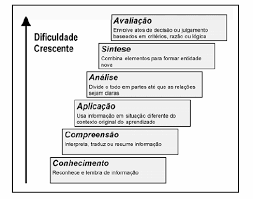
\includegraphics[width=0.7\textwidth]{figs/bloom1.png}
	\caption{N�veis de aprendizagem no dom�nio cognitivo}
	\label{bloom1}
\end{figure}


Cada um destes dom�nios tem diversos n�veis de profundidade de aprendizado. Por isso a classifica��o de Bloom � denominada hierarquia: cada n�vel � mais complexo e mais espec�fico que o anterior como mostrado na Figura \ref{bloom1}.

Os n�veis cognitivos de Bloom s�o usados para definir \textit{objetivos educacionais} de forma precisa. A Figura \ref{bloom2} mostra os verbos a serem usados para se definir objetivos educacionais para cada dos n�veis citados de acordo com a Taxonomia de Bloom.
 

\begin{figure}[h]
	\centering
	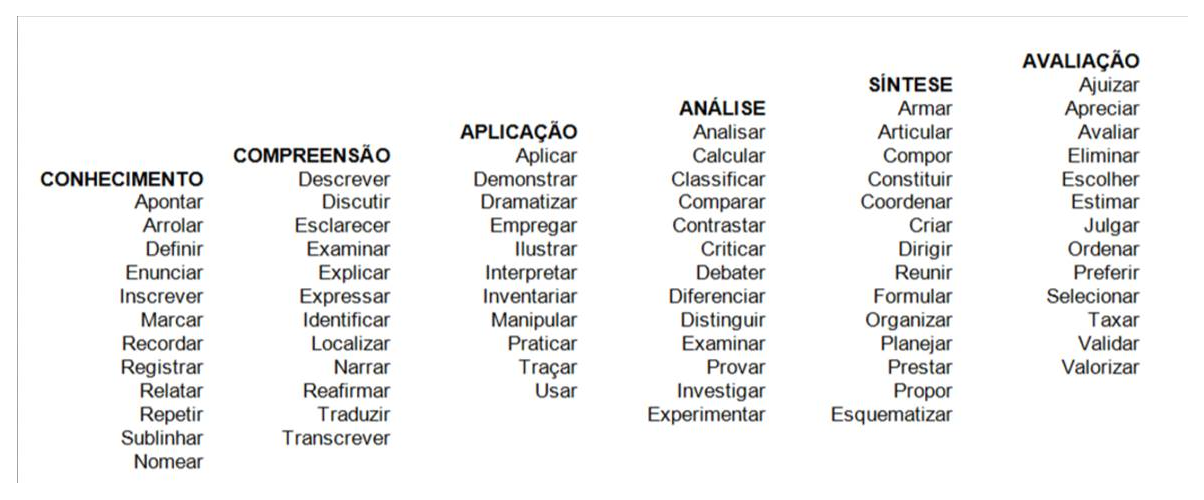
\includegraphics[width=0.7\textwidth]{figs/bloom2.eps}
	\caption{Verbos de descri��o de objetivos educacionais a serem usados em cada n�vel cognitivo.}
	\label{bloom2}
\end{figure}

Um objetivo educacional definido segundo a taxonomia de Bloom segue o seguinte padr�o: 
	
	"O(s) aluno(s) ser�(�o) capaz(es) de (\textbf{Verbo pr�prio do n�vel cognitivo considerado}) (\textbf{Conte�do estudado}).

Um exemplo de aplica��o para o caso de primeiro n�vel cognitivo, no estudado de equa��es diferenciais:

"O aluno ser� capaz de \textbf{definir} o que s�o \textbf{equa��es diferenciais}."

\subsubsection{Programa desenvolvido em QT para aux�lio na defini��o de objetivos educacionais}

Para este trabalho, foi criado um aplicativo na plataforma de programa��o QT\textsuperscript{\textregistered} para facilitar a defini��o de objetivos educacionais de acordo com a Taxonomia de Bloom. 

\begin{figure}[H]
	\centering
	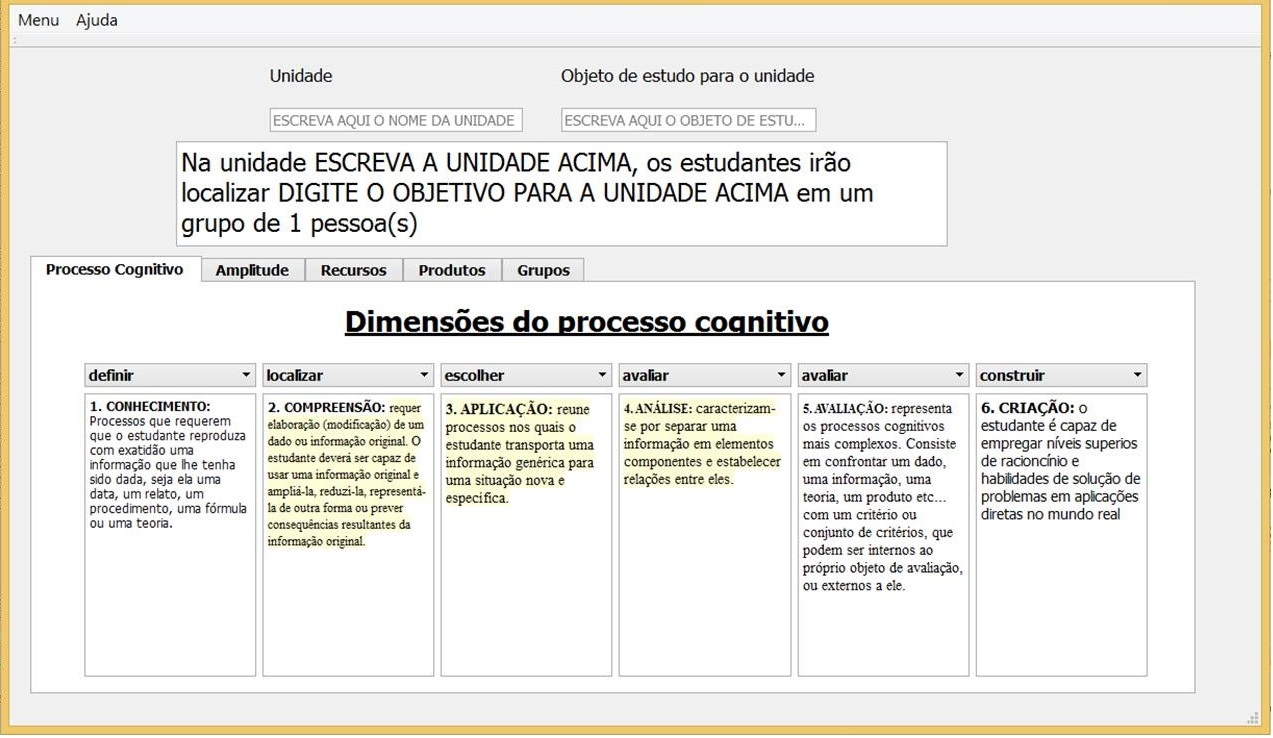
\includegraphics[width=1\textwidth]{figs/app2.jpg}
	\caption{Tela inicial do aplicativo desenvolvido em QT para definir os objetivos educacionais.}
	\label{app2}
\end{figure}

A Figura \ref{app2} mostra a tela inicial do aplicativo desenvolvido. Na regi�o de inser��o de texto Descrita por \textbf{Unidade}, deve-se escrever de qual unidade de ensino se est� tratando. Na regi�o textual central, marcada na Figura  \ref{app2_1}, � mostrado resultado do objetivo educacional definido.

\begin{figure}[H]
	\centering
	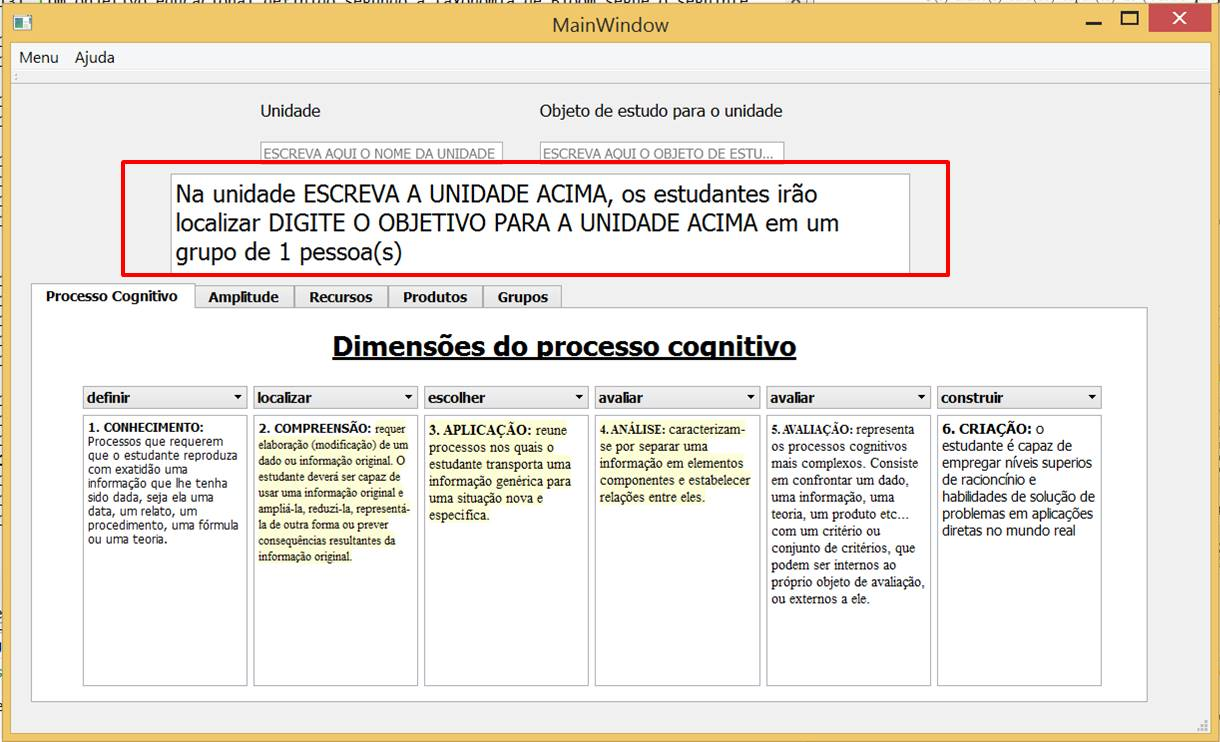
\includegraphics[width=1\textwidth]{figs/app2_1.jpg}
	\caption{Tela inicial do aplicativo desenvolvido em QT para definir os objetivos educacionais, ret�ngulo vermelho marcando a regi�o onde o objetivo educacional definido � mostrado.}
	\label{app2_1}
\end{figure}

A Figura \ref{app3} mostra o resultado, na regi�o textual central , da defini��o do \textbf{Unidade}. 

\begin{figure}[H]
	\centering
	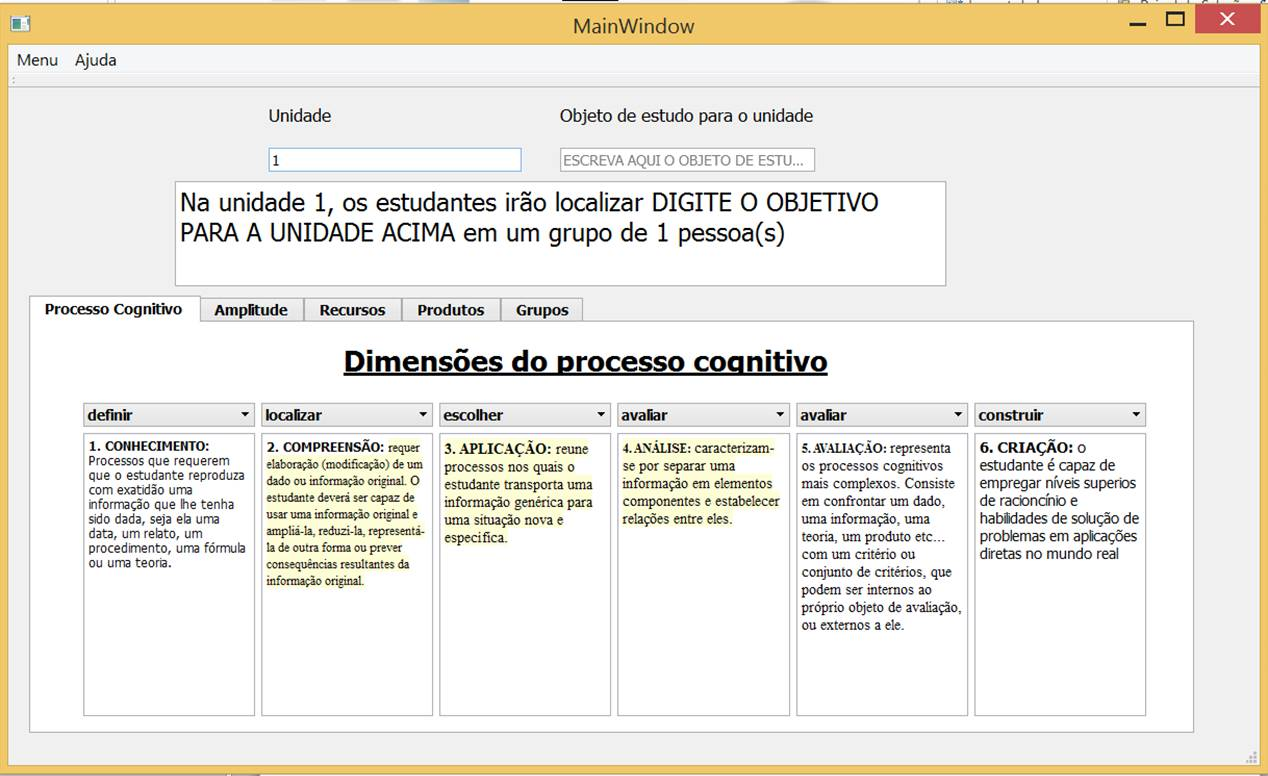
\includegraphics[width=1\textwidth]{figs/app3.jpg}
	\caption{Definindo uma unidade de ensino.}
	\label{app3}
\end{figure}

A Figura \ref{app4} mostra o resultado, na regi�o textual central , da defini��o do \textbf{Objeto de estudo} espec�fico para a \textbf{Unidade} definida. 

\begin{figure}[H]
	\centering
	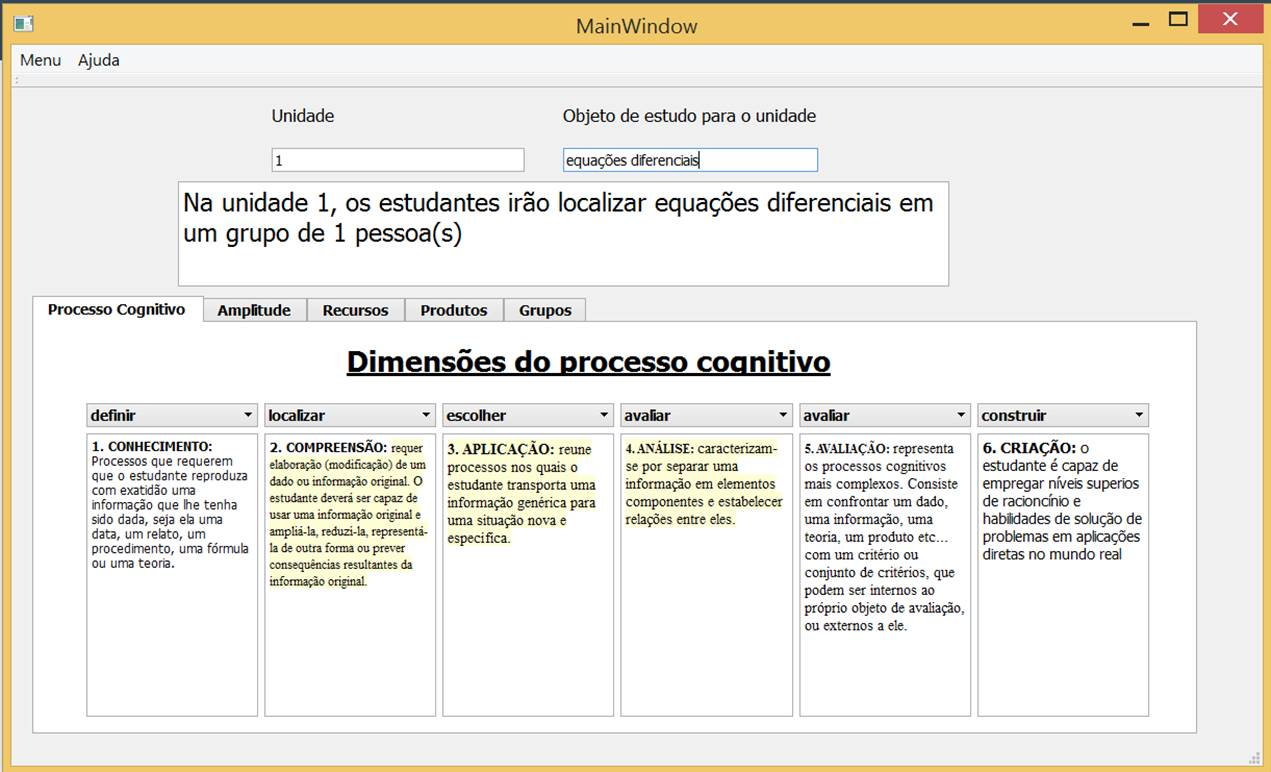
\includegraphics[width=0.7\textwidth]{figs/app4.jpg}
	\caption{Definindo um objetivo de estudo para a unidade de estudo.}
	\label{app4}
\end{figure}

A Figura \ref{app4_1} mostra os n�veis do processos cognitivos da Taxonomia de Bloom.
\begin{figure}[H]
	\centering
	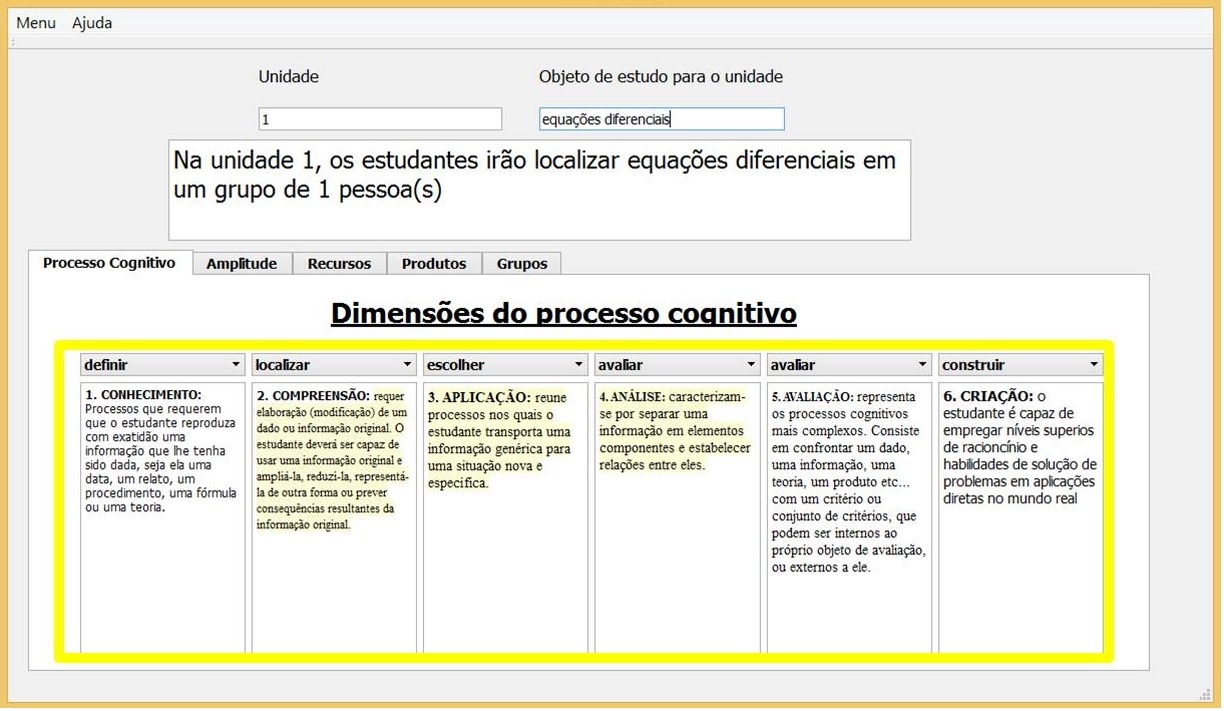
\includegraphics[width=1\textwidth]{figs/app4_1.jpg}
	\caption{Ret�ngulo amarelo destacando os n�veis cognitivos.}
	\label{app4_1}
\end{figure}

Cada \textit{Combo-box} mostrado possui os verbos associados a cada n�vel cognitivo. Quando um verbo � selecioando, o objetivo educacional exposto na regi�o retangular � alterado, como exposto na Figura \ref{app5_2}.

\begin{figure}[H]
	\centering
	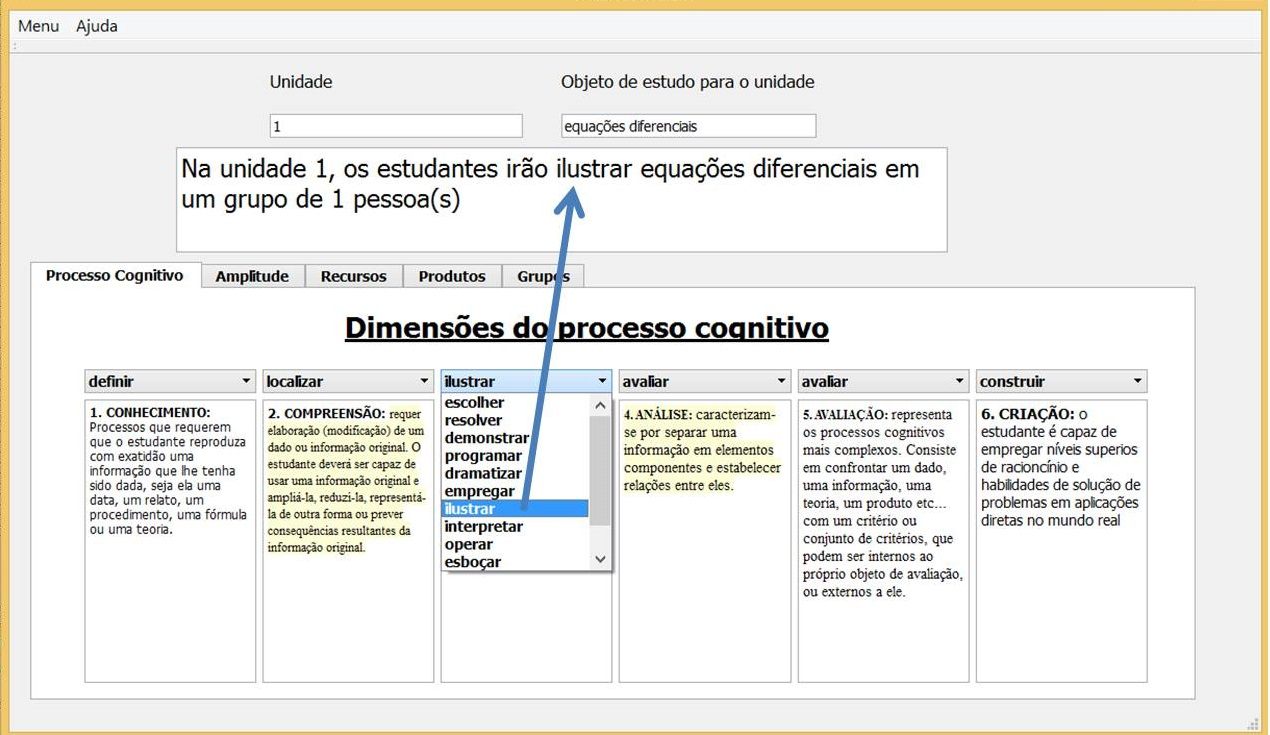
\includegraphics[width=0.9\textwidth]{figs/app5_2.jpg}
	\caption{Selecionando um verbo de um n�vel cognitivo.}
	\label{app5_2}
\end{figure}

Na aba \textit{Amplitude}, s�o selecionados modificadores para especifica��o do objetivo educacional. A Figura \ref{app6} mostra o uso do modificador para alterar o objetivo educacional adicionando o modificador "o objetivo geral".

\begin{figure}[H]
	\centering
	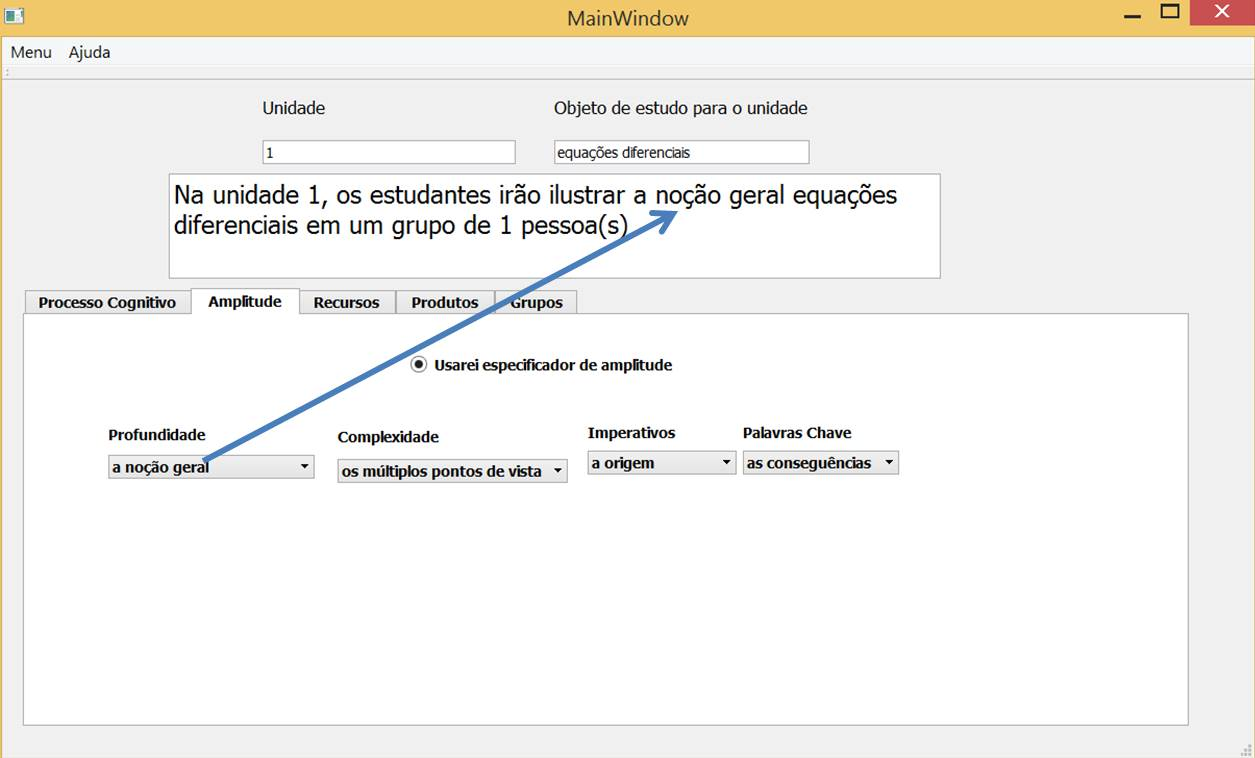
\includegraphics[width=0.9\textwidth]{figs/app6.jpg}
	\caption{Selecionando a amplitude do estudo a ser realizado.}
	\label{app6}
\end{figure}

Na aba \textit{Recursos}, s�o especificados recursos com os quais os estudantes realizar�o atividades em dire��o � masteriza��o do conte�do. A Figura \ref{app7} mostra o uso do especificador para alterar o objetivo educacional adicionando o recurso "livro".

\begin{figure}[H]
	\centering
	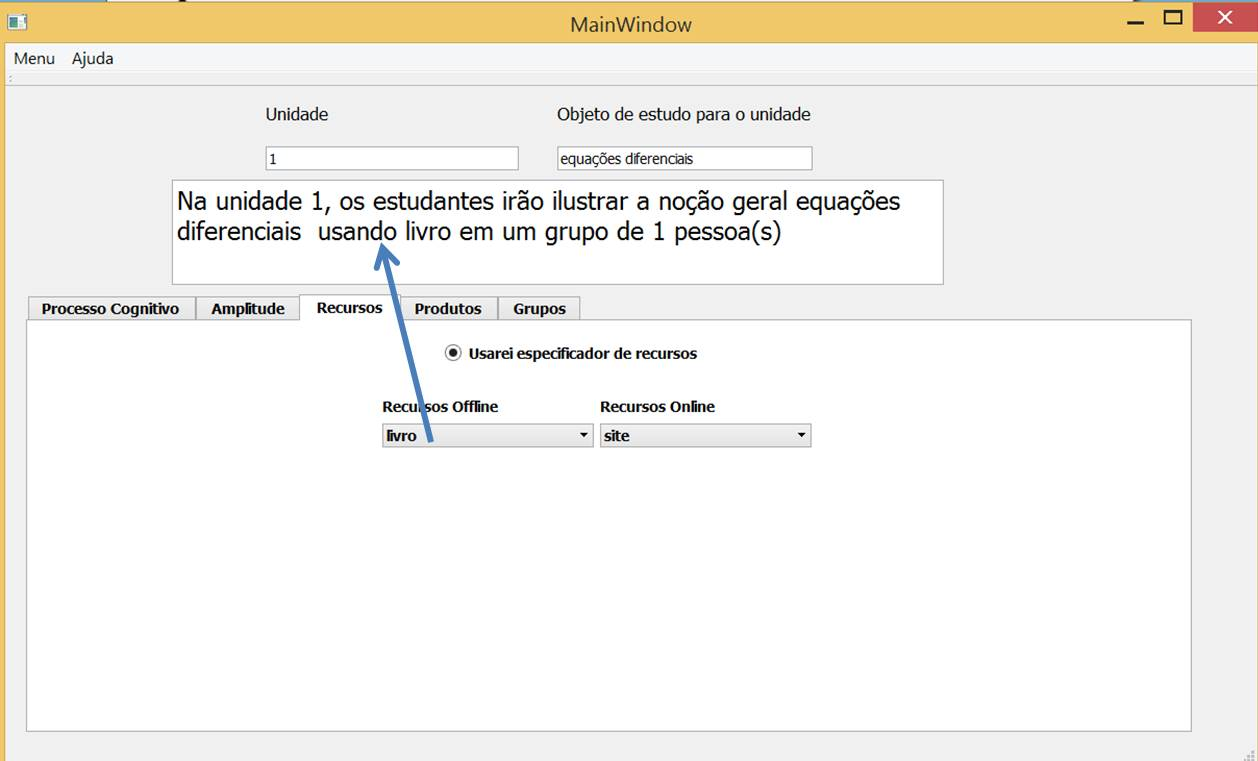
\includegraphics[width=0.9\textwidth]{figs/app7_3.jpg}
	\caption{Selecionando o recursos a ser utilizado para alcan�ar o obejtivo educacional especificado.}
	\label{app7_3}
\end{figure}

Na aba \textit{Produtos}, � especificado o que os alunos desenvolver�o para atingir o objetivo educacional especificado. A Figura \ref{app8} mostra o uso do especificador de produto a ser desenvolvido para alterar o objetivo educacional adicionando o objetivo de produzir um "artigo".


\begin{figure}[H]
	\centering
	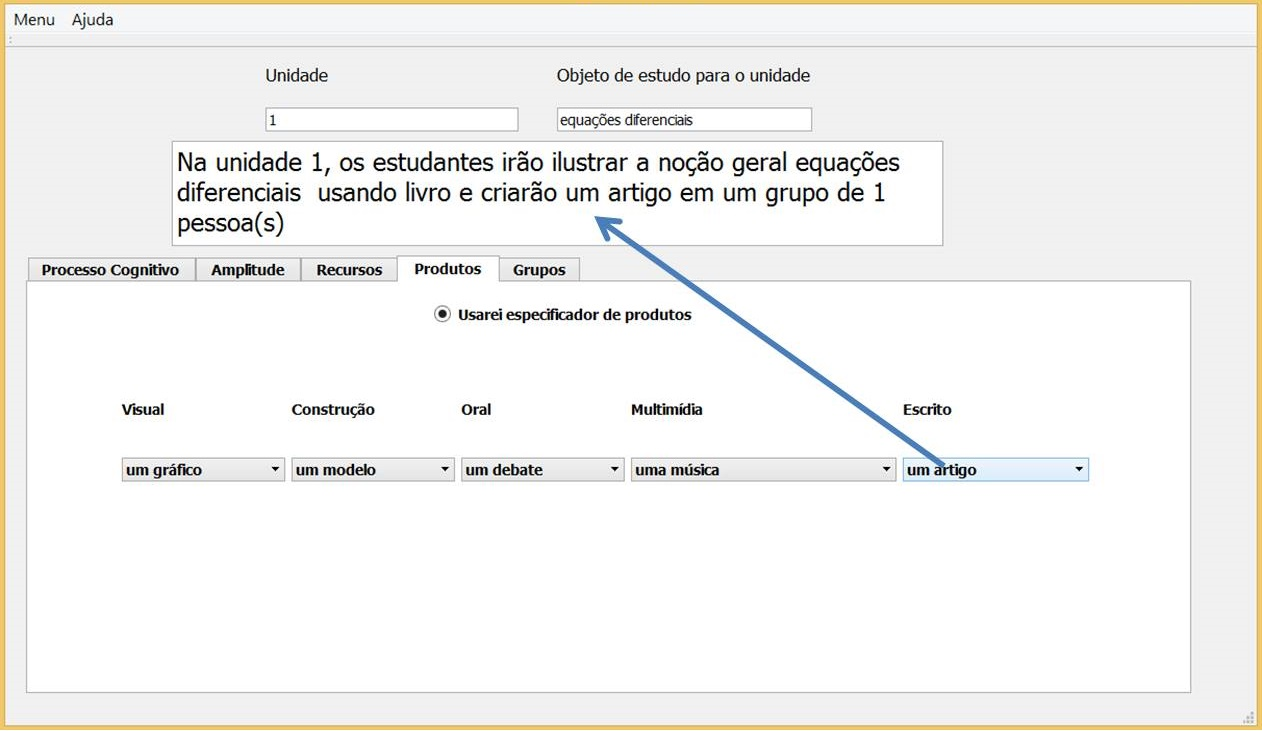
\includegraphics[width=0.9\textwidth]{figs/app8.jpg}
	\caption{Selecionando um produto a ser desenvolvido como atividade de masteriza��o.}
	\label{app8}
\end{figure}

Finalmente, na aba \textit{Grupos}, � especificado a quantidade de alunos por grupo que realizar�o, conjuntamente as atividades de masteriza��o. A Figura \ref{app9} mostra  a altera��o da quantidade de pessoas por grupo para, por exemplo, 4 pessoas.
\begin{figure}[H]
	\centering
	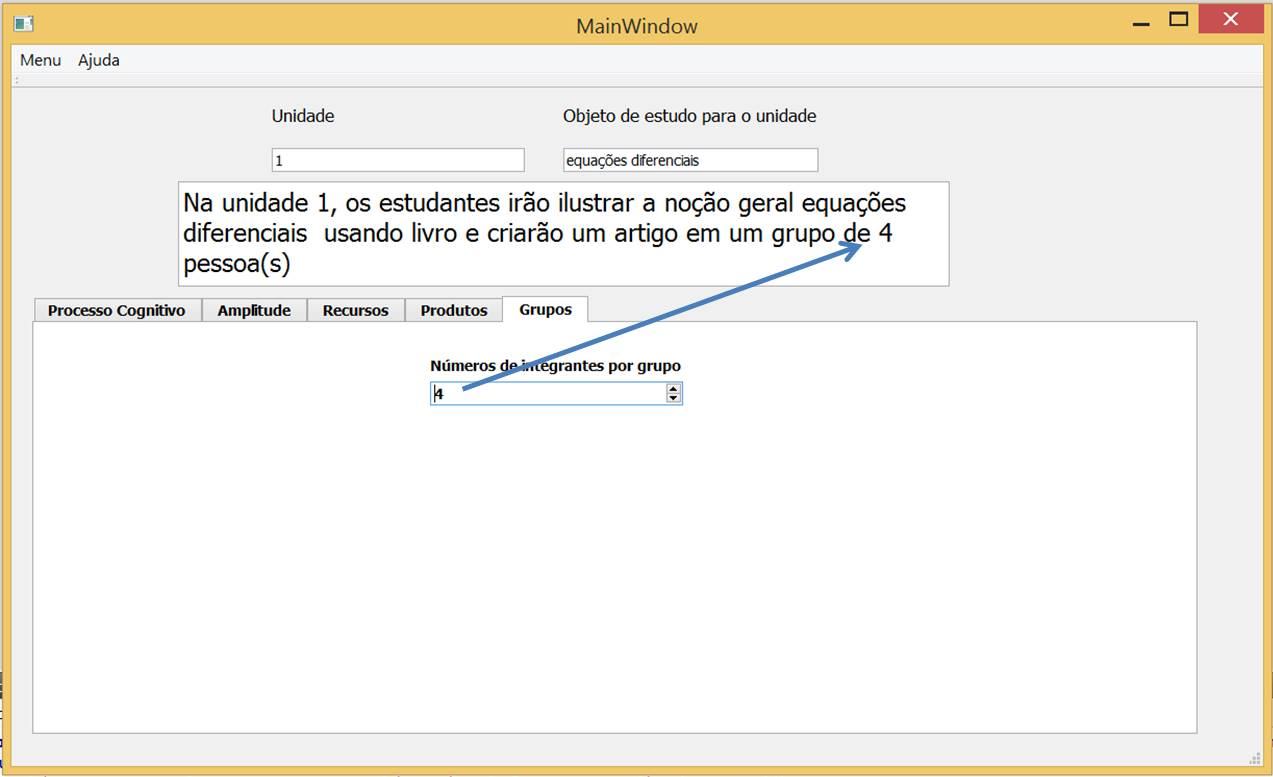
\includegraphics[width=0.9\textwidth]{figs/app9.jpg}
	\caption{Selecionando a quantidade de pessoas por grupo.}
	\label{app9}
\end{figure}




\section{Metodologias para desenvolvimento de projetos }
\label{EstudoScrum}

Scrum � um metodologia �gil de densenvolvimento de projeto que surgiu no contexto de engenharia de software. O termo �gil se aplica nesse contexto para ser um contraste a metodologia em \textit{Cascata} (metodologia cl�ssica) de desenvolvimento de projetos de software. Enquanto na metodologia \textit{Cascata}, foca-se principalmente em \textit{processos} e na obedi�ncia a eles, na metodologia Scrum, foca-se na \textit{melhora cont�nua} e \textit{entrega constante de valor}.

Apesar de suas origens, tanto a metodologia em \textit{Cascata} com o \textit{Scrum} s�o amplamente utilizados no mais diversos campos.

Nesta se��o, descreve-se as rapidamente a metodologia de desenvolvimento de projetos \textit{Cascata}, para depois apresentar uma descri��o detalhada da metodologia de desenvolvimento de projetos \textit{Scrum}, a qual � a metodologia a ser aplicada no curso \textit{Algoritmos e Programa��o de Computadores} proposto.

\subsection{Metodologia Cascata}
\label{SecCascata}
A Figura \ref{scrum4} mostra a um breve resumo das fases que devem ser obedecidas na metodologia de desenvolvimento de projetos \textit{Cascata}. S�o elas:
  
\begin{figure}[H]
	\centering
	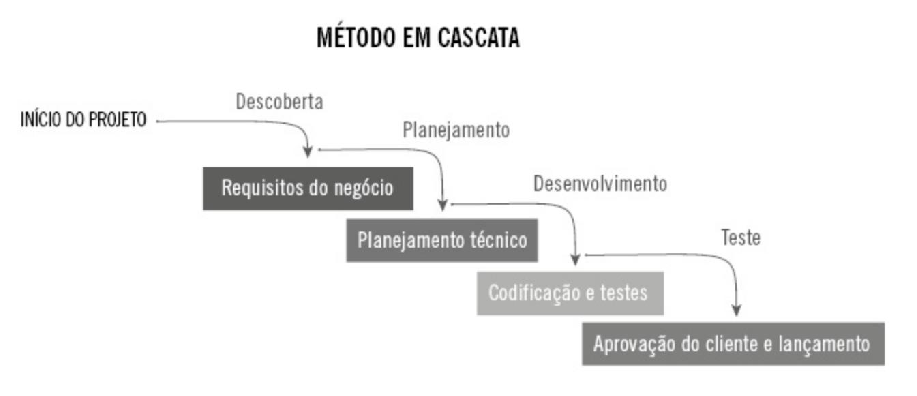
\includegraphics[width=0.7\textwidth]{figs/Scrum4.eps}
	\caption{Fluxo da metodologia de desenvolvimento de projeto \textit{Cascata}}
	\label{scrum4}
\end{figure}


\begin{enumerate}
	\item Anal�se e descoberta de requisitos de neg�cio
	\item Planejamento de produto (Design)
	\item Implementa��o (codifica��o)
	\item Testes
	\item Entrega do produto ao cliente (instala��o)
	\item Manuten��o
\end{enumerate}	

 Todas etapas mostrada nessa figura s�o seguenciais planejadas extensivamente pela equipe de projeto, produzindo, nesse intervalo entre etapas, um conjunto amplo de documentos.
 
Muitos argumentam que a metodologia em \textit{Cascata} torna o desenvolvimento do projeto muito engessado \cite{artigoCascada}. Os pontos positivos e negativos da metodologia de desenvolvimento de projeto \textit{Cascata} s�o mostrados na tabela \ref{tabCascata}.

\begin{table}[]
	\centering
	\caption{Pontos positivos e negativos da metodologia de desenvolvimento de projetos \textit{Cascata}}
	\label{tabCascata}
	\begin{tabular}{|l|l|}
		\hline
		\textbf{Pontos positivos}                                                                                                                                   & \textbf{Pontos negativos}                                                                                                                                        \\ \hline
		Documenta��o detalhada                                                                                                                                      & Come�o de projeto lento                                                                                                                                          \\ \hline
		\begin{tabular}[c]{@{}l@{}}Requerimentos de projeto\\ totalmente colhidos e acor-\\ dados no in�cio do projeto\end{tabular}                                 & \begin{tabular}[c]{@{}l@{}}Requerimentos fixos e \\ dificilmente modific�veis\end{tabular}                                                                       \\ \hline
		\begin{tabular}[c]{@{}l@{}}O projeto pode ser desenvolvi-\\ do por pessoas ainda inexperi-\\ entes.\end{tabular}                                            & \begin{tabular}[c]{@{}l@{}}Sem acompanhamento do\\ projeto pelo cliente e outros\\ stakeholders at� o projeto\\ estar conclu�do\end{tabular}                       \\ \hline
		\begin{tabular}[c]{@{}l@{}}N�mero de defeitos reduzido\\ por meio de planejamento e \\ desenvolvimento mais rigoroso\end{tabular}                           & \begin{tabular}[c]{@{}l@{}}Pouca flexibilidade para mudar\\  a dire��o e modus-operandi do\\ projeto.\end{tabular}                                               \\ \hline
		\begin{tabular}[c]{@{}l@{}}In�cio e fim de cada est�gio ple-\\ namente definidos, permitindo\\ acompanhamento mais eficien-\\ te do progresso.\end{tabular} & \begin{tabular}[c]{@{}l@{}}Clientes e Stakeholders possi-\\ velmente podem alterar os requi-\\ sitos de projeto ap�s a fase de \\ in�cio de projeto\end{tabular} \\ \hline
	\end{tabular}
\end{table}

O principal problema, pontuado por pesquisadores \cite{artigoCascada2}, quanto � metodologia \textit{Cascata}, �, como mostrado na tabela \ref{tabCascata} a falta de dinamicidade, especialmente quanto a defini��o de pre-requisitos de projeto. Uma vez que a primeira fase do projeto, colhimento de requisitos, � conclu�da, n�o mais os requisitos s�o revistos. Isso causa, muitos problemas de retrabalho , em especial, nas fases finais e atrasos grandes.


\subsection{Metodologia  Scrum}
\label{secScrum}

A metodologia \textit{Scrum} de gerenciamento de projeto surgiu como contraste � metodologia \textit{Cascata} tratada na se��o \ref{SecCascata} sendo uma metodologia �gil de desenvolvimento de projetos. 


A metodologogia Scrum � uma metodologia a ser desenvolvida em pequenas equipes, chamadas \textit{Time ou Equipe Scrum} e umas de suas principais caracter�sticas s�o a revis�o frequente dos \textbf{\textit{requisitos de projeto}}, a melhora cont�nua e o \textbf{\textit{acr�scimo de valor direto}} acima da obedici�ncia a cronogramas e processos (Pr�prios de metodologias similares a metodologia Cascata).



 
\begin{figure}[h]
	\centering
	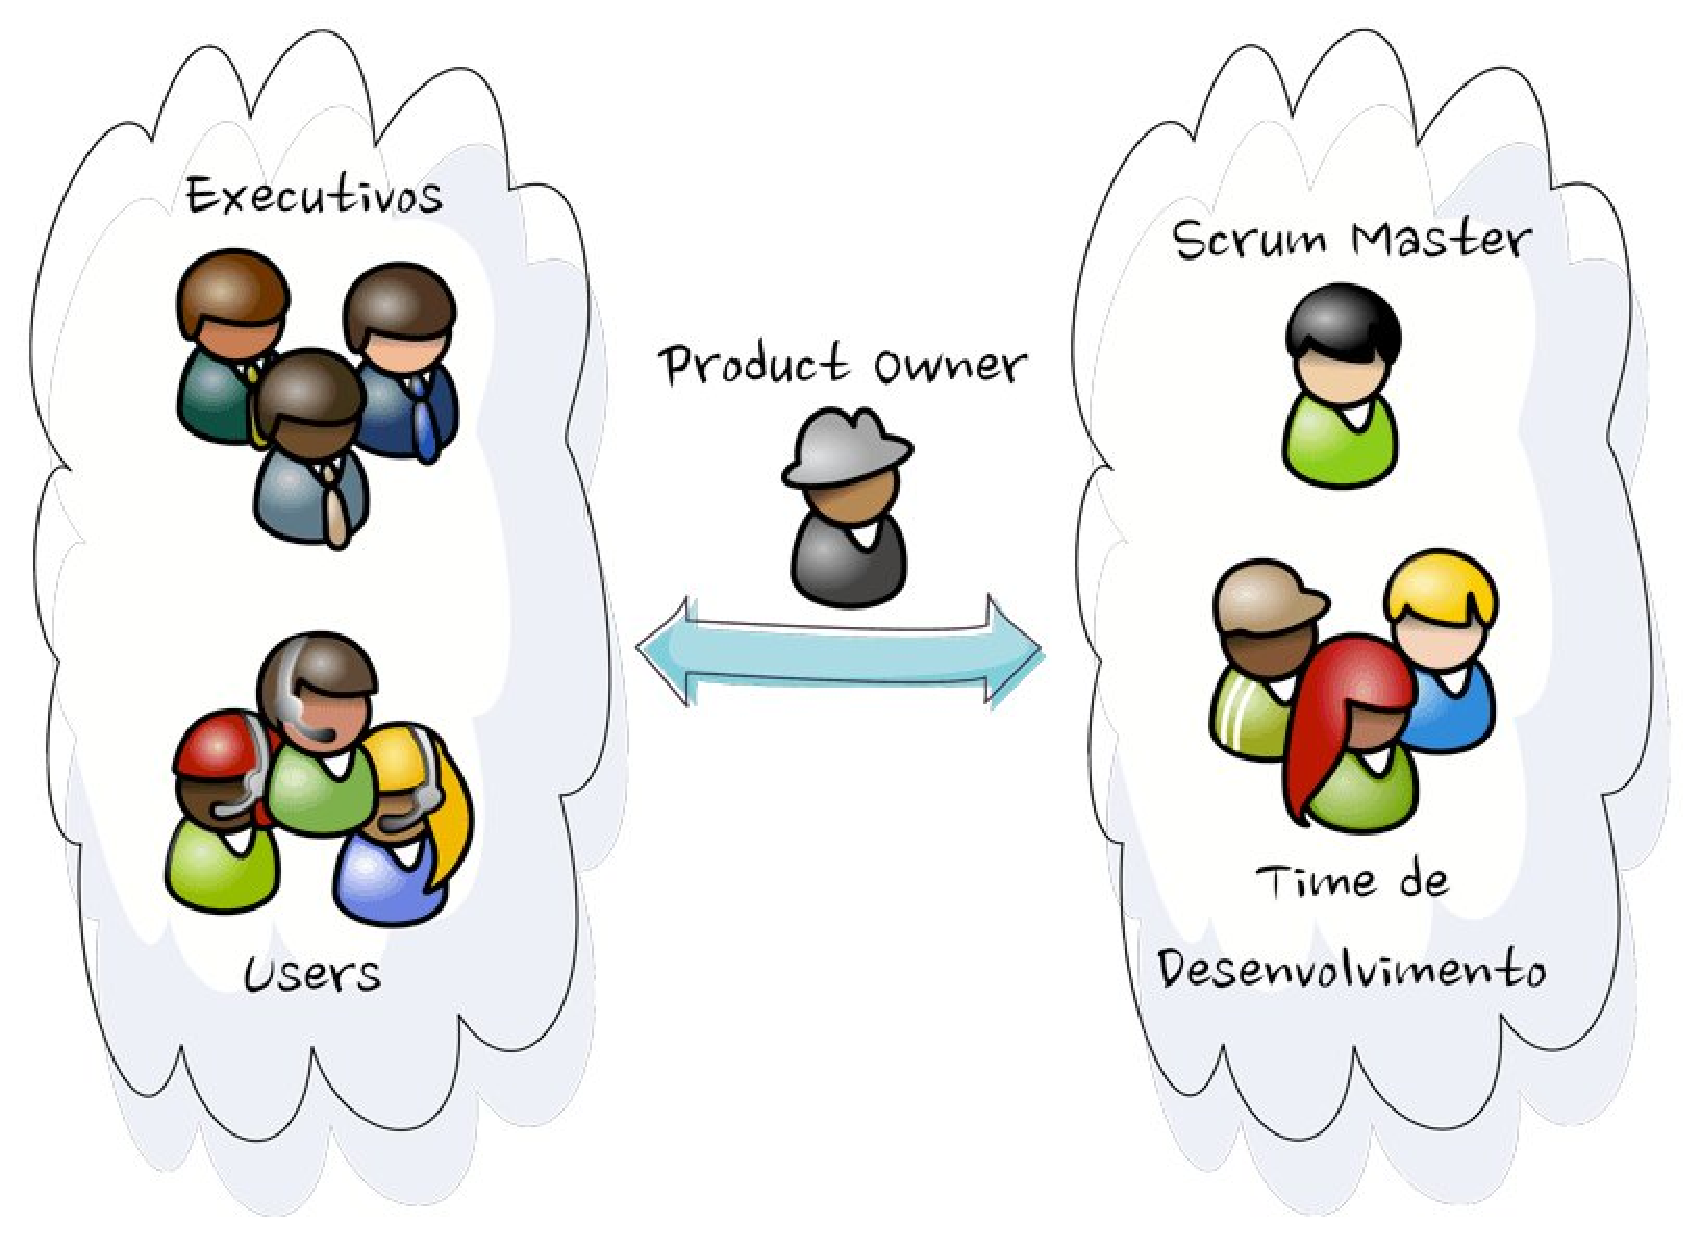
\includegraphics[width=0.5\textwidth]{figs/SCRUM6.eps}
	\caption{Papel \textit{Product Owner}, metodologia \textit{Scrum}}
	\label{scrum6}
\end{figure}


Os pap�is, na metodologia Scrum, s�o os seguintes:

\begin{itemize}
	
	\item \textbf{\textit{Scrum Master}}: O \textit{Scrum Master} � o respons�vel por manter a \textit{Equipe Scrum} nas diretrizes do processo Scrum. Ele deve treinar e orientar os demais participantes. Al�m disso, ele � respons�vel por  proteger a equipe Scrum de pertuba��es externas alheias ao projeto incentivando tal equipe na tomada de decis�es para torna-l� progressivamente mais auto-gerenci�vel. Com rela��o a todos envolvidos no projeto, al�m da equipe Scrum, o \textit{Scrum Master} deve zelar pela visibilidade do progresso do projeto para que a verifica��o e ger�ncia sejam processos compartilhados.
	
	\item \textit{\textbf{Product Owner}}: O \textit{Product Owner} � representa a "voz do cliente". Como a Figura \ref{scrum6} mostra, o \textit{Product Owner}  atua como "ponte" ente a equipe desenvolvimento e os \textit{Stakeholders (Pessoa com interesse direto no produto)}. Ele deve entender as necessidades e prioridades dos \textit{Stakeholders} e passar claramente os \textit{\textbf{crit�rios de aceita��o}} para a equipe de desenvolvimento 
	
	 \item \textbf{\textit{Equipe Scrum}}: 	As  equipes Scrum s�o auto-organizadas e multidisciplinares. Como tal, ela deve escolher a melhor forma de desenvolver seus trabalhos ao inv�s de serem comandadas por outros de fora da equipe. Equipes multidisciplinares possuem todas as compet�ncias necess�rias para desenvolverem seus trabalhos sem dependerem de outros que n�o fazem parte da Equipe Scrum. O modelo da Equipe Scrum � desenvolvido para otimizar a flexibilidade, criatividade e produtividade.
	 
	 Equipes Scrum entregam produtos iterativamente e incrementalmente maximizando a oportunidade de feedback. Entregas incremetais de produto "pronto" garantem que uma vers�o do produto potencialmente utiliz�vel est� sempre dispon�vel para uso.

	
\end{itemize}

\begin{figure}[h]
	\centering
	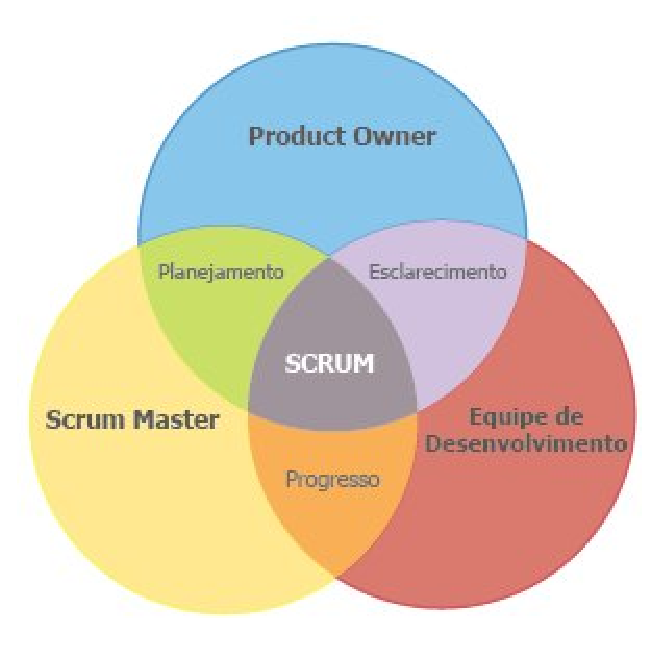
\includegraphics[width=0.5\textwidth]{figs/scrum7.eps}
	\caption{Metodologia Scrum, intersec��o entre os pap�is}
	\label{scrum7}
\end{figure}

A Figura \ref{scrum7} mostra a intersec��o entre os pap�is da metodologia Scrum de acordo com suas respectivas tarefas. 

A Figura \ref{scrum3} mostra em resumo o fluxo a ser estabelecido na metodologia Scrum. Tal fluxo segue a seguinte enumera��o:

\begin{figure}[H]
	\centering
	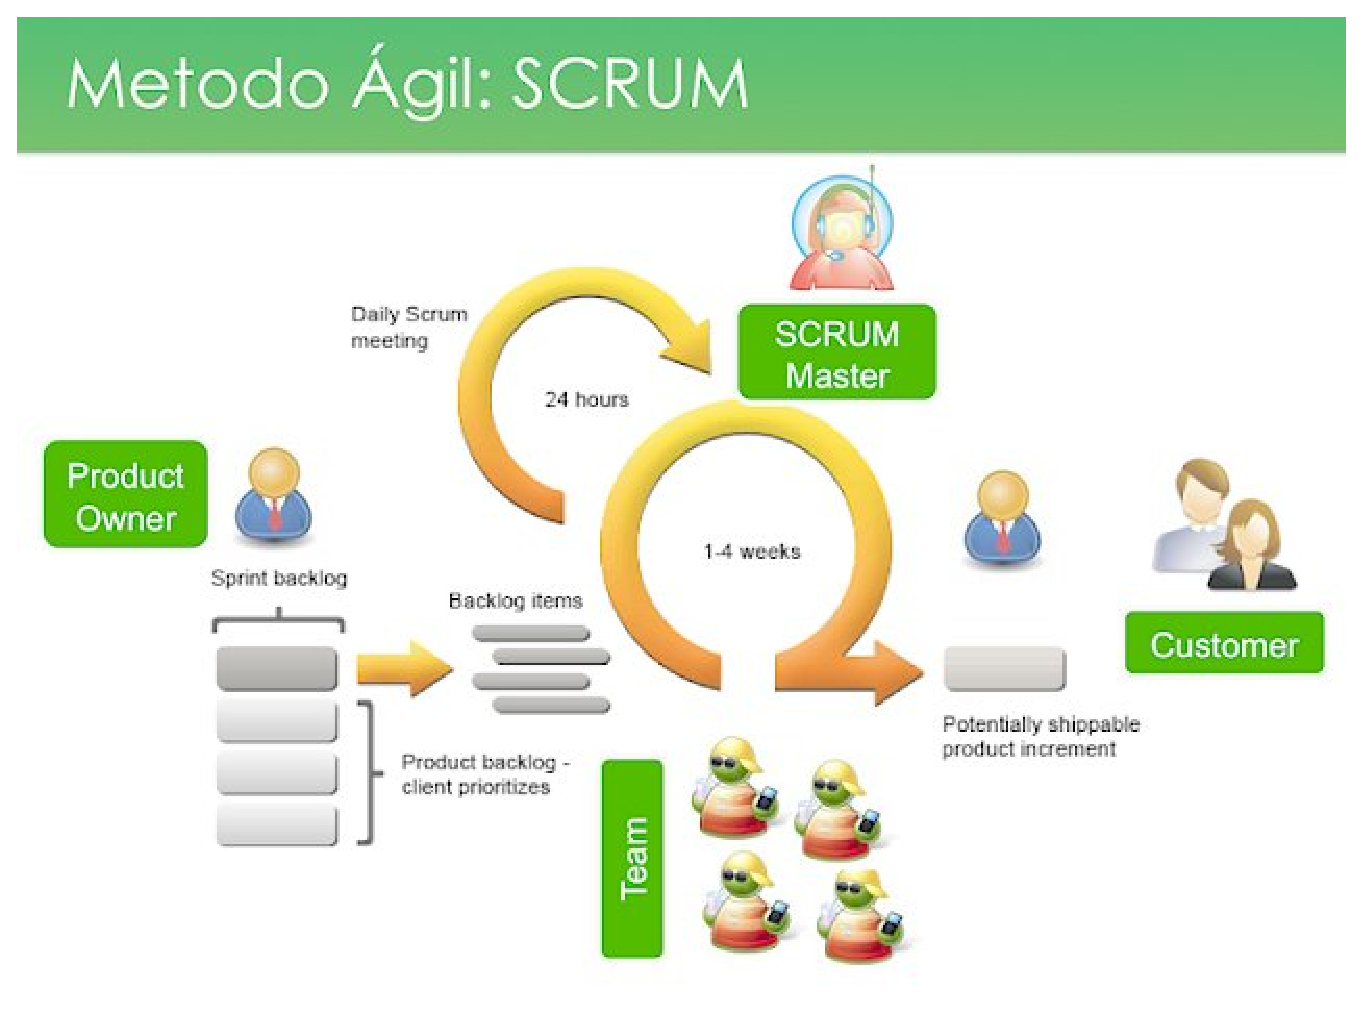
\includegraphics[width=0.5\textwidth]{figs/Scrum3.eps}
	\caption{Fluxo da metodologia Scrum}
	\label{scrum3}
\end{figure}

\begin{itemize}
	\item \textbf{Fase 1  - In�cio}: Para a  fase inicial de um projeto Scrum, devem se desenvolvidas as seguintes passos:
	    \subitem \textbf{1.1)Criar Vis�o de Projeto}:
		Descri��o da necessidade ou desejo dos clientes e as caracter�sticas do produto que resolvem as necessidades. Sendo elas necessidades relacionadas a:
		    \subsubitem	\textbf{Caracter�sticas funcionais}:   
				Caracter�sticas que descrevem uma funcionalidade direta do produto. 
			\subsubitem \textbf{Caracter�sticas n�o funcionais}
				Caracter�sticas ligadas a efici�ncia e efic�cia do produto ao realizar uma de suas caracter�stica funcionais. 
	
			\subitem 1.2) Para descrever as necessidades ou desejo dos clientes, devem ser criadas \textit{User Stories} no formato:
		"Como um (\textbf{\textit{Tipo de Usu�rio}}), eu quero, poder fazer (\textbf{\textit{Caracter�stica Funcional}})". 
	
	\item \textbf{Fase 2  - Plano de Projeto e Estima��es}:
	
		\subitem 2.1) Crit�rios de aceita��o s�o criados (a ser feito pelo Product Owner juntamente com o Scrum Team).
		\subitem 2.2) Scrum Master e time estimam o esfor�o necess�rio para desenvolver as User Stories.
		\subitem 2.3) Scrum master e time se comprometem a desenvolver o produto de acordo com as Epics(Conjunto de User Stories) e crit�rios de aceita��o.
		\subitem 2.4) User Stories s�o divididas em subtarefas para criar uma Task List.
		\subitem 2.5) Time Scrum se reune para decidir quais tarefas ser�o realizadas na Sprint (Sprint Backlog).
		
	
	\item \textbf{Fase 3  - Implementa��o}:
		
		Na fase de implementa��o, o trabalho � dividido em ciclos curtos de trabalho, de 1 a 4 semanas de dura��o, como mostrado na Figura \ref{scrum2}. Esse ciclos s�o chamados de \textit{Sprints}. Cada Sprint tem sua lista de tarefas( \textit{Task List}) pr�pria.
		
		As responsabilidades da Equipe Scrum na Fase 3, s�o as seguintes: 
	
	\subitem 3.1) Criar os "entreg�veis" do SPRINT.  
	\subitem 3.2) Realizar reuni�es di�rias r�pidas de no m�ximo 15 minutos para discutir problemas e progresso.       
	\subitem 3.3) Atualizar o quadro Scrum de ( A FAZER , FAZENDO, FEITO) a cada dia de trabalho.
	
	
	\item \textbf{Fase 4  - Revis�o e Retrospecto }:
	
	A fase de \textit{Revis�o e Retrospecto} � realizada ao final de cada Sprint. As responsabilidades da equipe Scrum na Fase 4 s�o"
	
	\subitem 4.1) Os entreg�veis do Sprint s�o mostrados para os Stakeholders.
	\subitem 4.2) Essas reuni�es s�o feitas para garantir a aprova��o do produto desenvolvido e fazer os ajustes necess�rios o mais r�pido poss�vel.                                               
	\subitem 4.3) O Scrum Master e o time Scrum se reunem para discutir o que foi aprendido no Sprint.
	\subitem 4.4) Informa��o � documentada para futuros Sprints.                                                    
	
\end{itemize}


Ap�s a conclus�o dessas 4 fases, o projeto Scrum chega a sua finaliza��o. As informa��es colhidas a cada Sprint s�o guardadas para projetos Scrum futuros.


\begin{figure}[H]
	\centering
	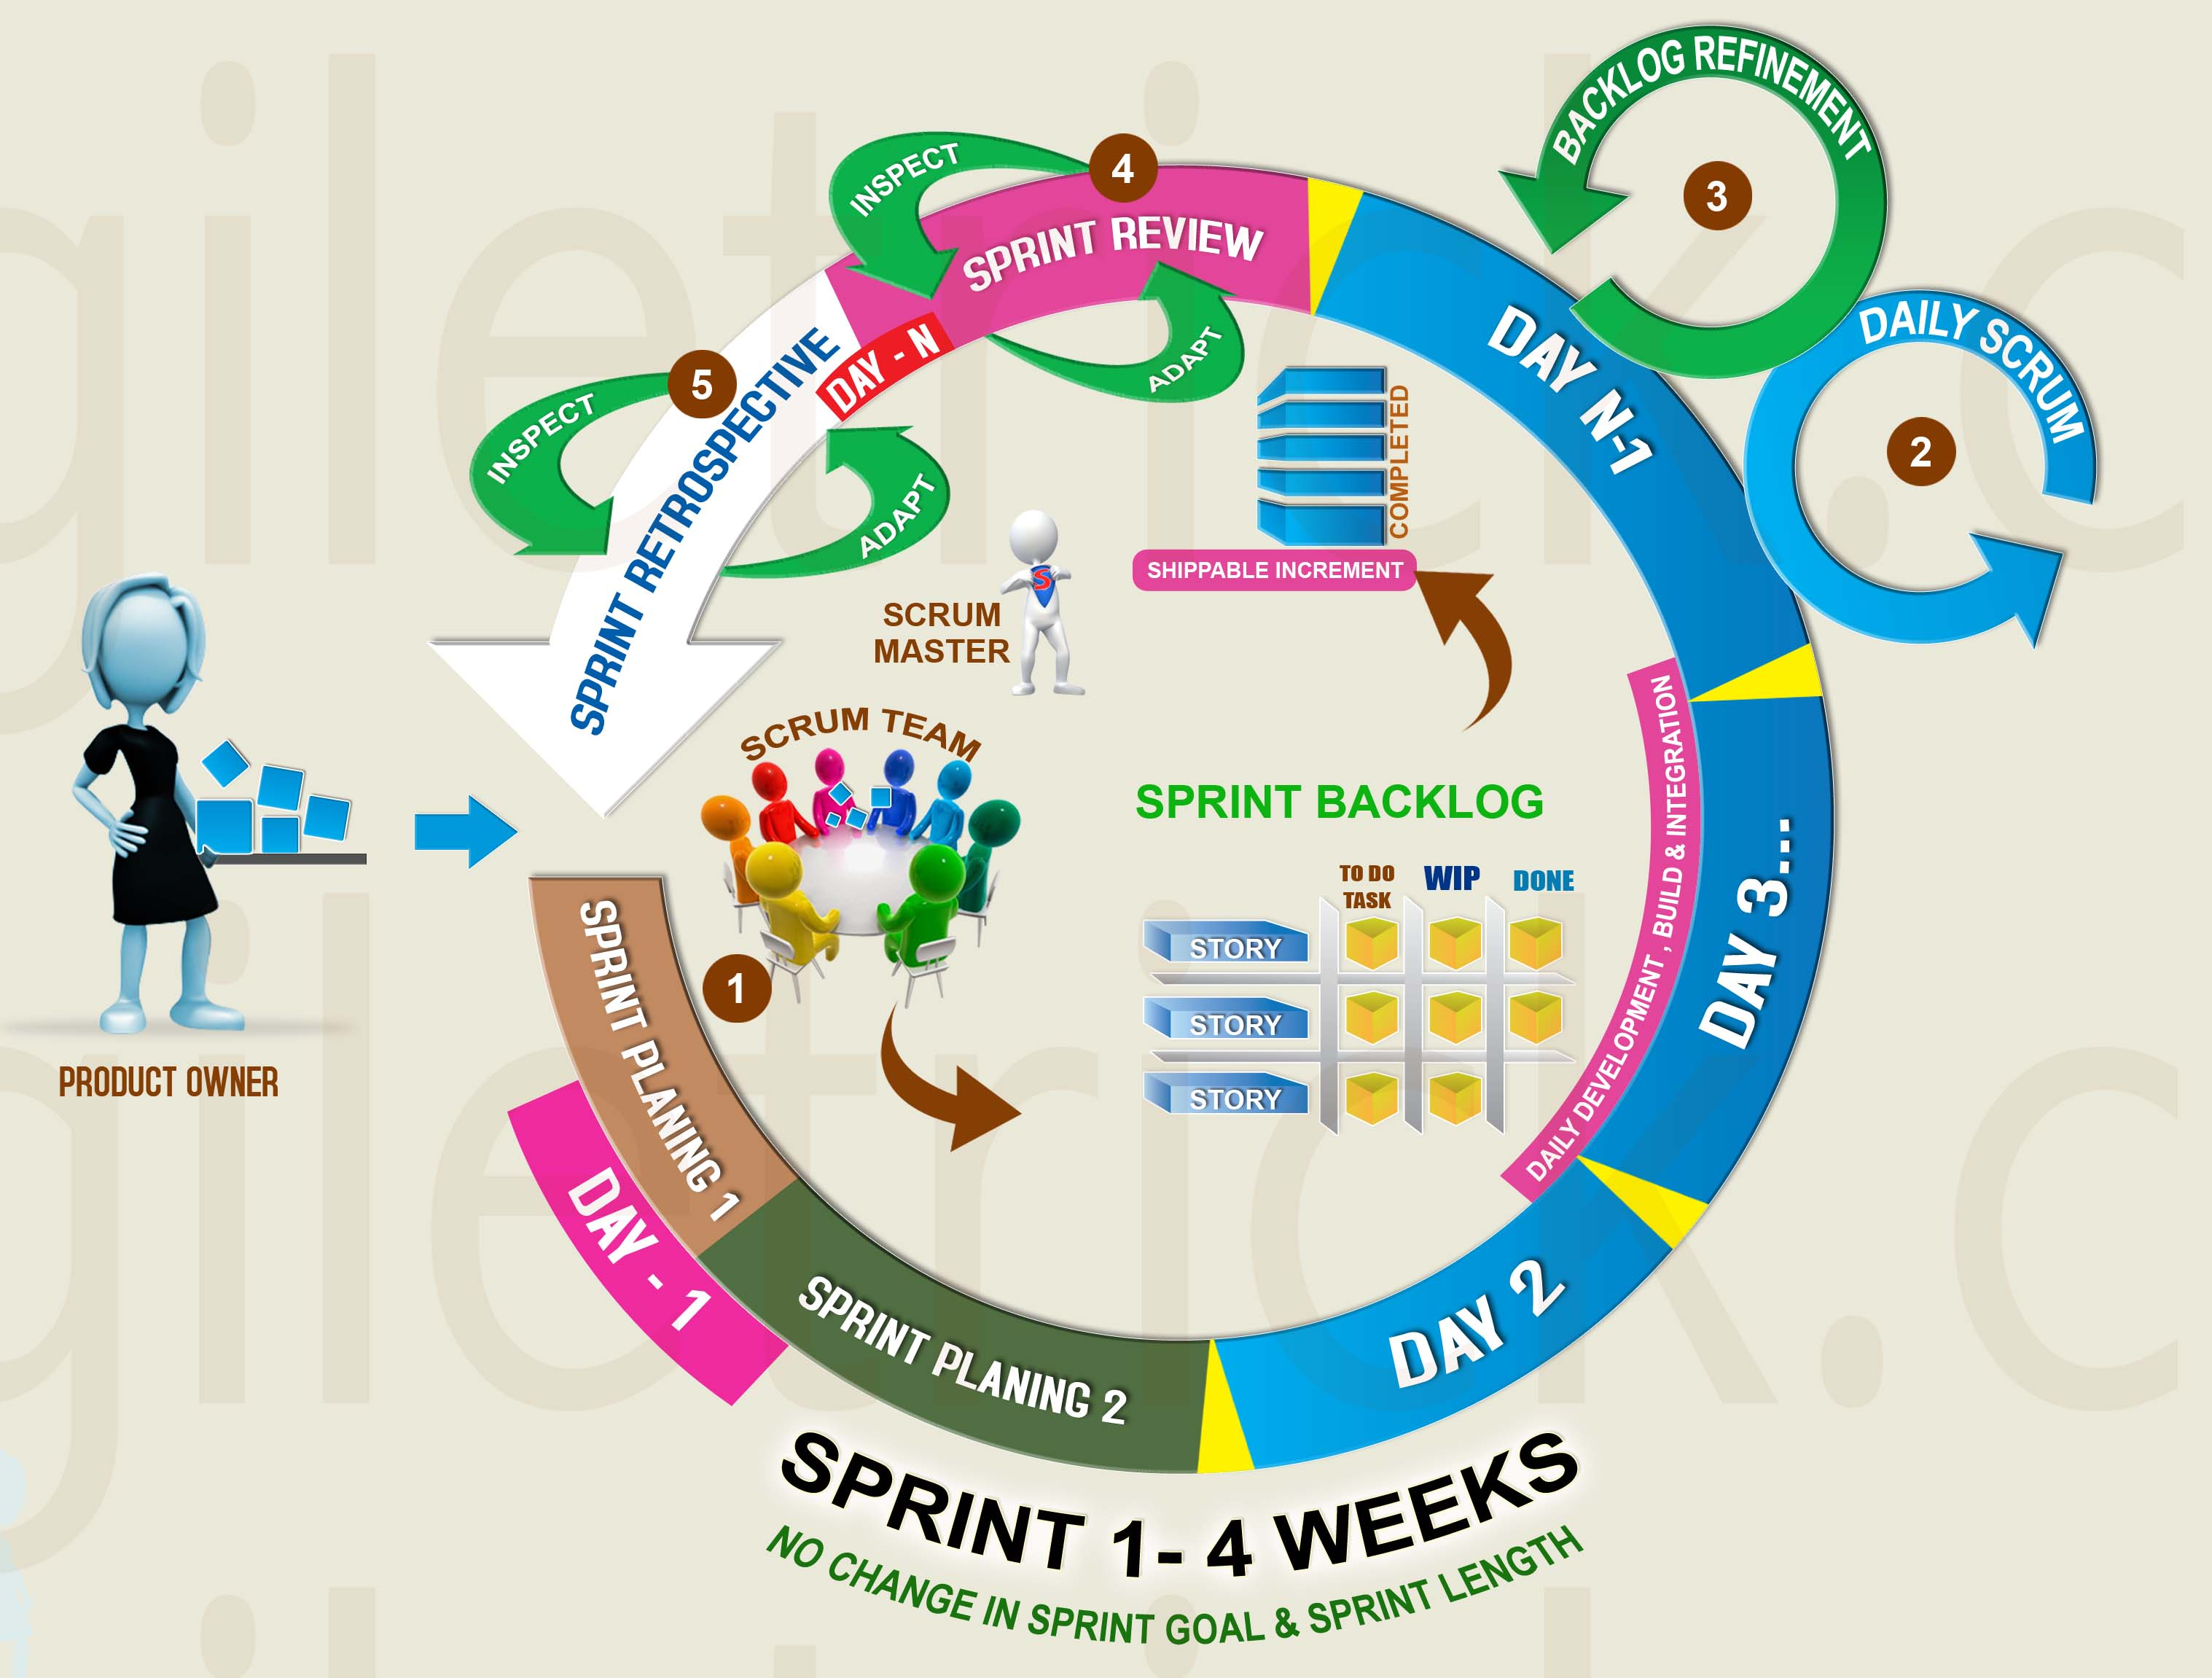
\includegraphics[width=0.5\textwidth]{figs/scrum2.eps}
	\caption{Fluxo de um Sprint dentro da metodologia Scrum}
	\label{scrum2}
	\source{agilelucero.com}
\end{figure}


A tabela \ref{tabScrum} faz um resumo dos pontos positivos e negativos pr�prios de metologias �geis de desenvolvimento de projeto, como a metodologia Scrum.

\begin{table}[]
	\centering
	\caption{Pontos positivos e negativos da metodologia de desenvolvimento de projetos \textit{Scrum}}
	\label{tabScrum}
	\begin{tabular}{|l|l|}
		\hline
		\textbf{Pontos positivos}                                                                                                                                    & \textbf{Pontos negativos}                                                                                                                \\ \hline
		\begin{tabular}[c]{@{}l@{}}In�cio r�pido, entrega de produto \\ realizada incrementalmente com \\ revis�o de clientes e feedback fre-\\ quentes\end{tabular} & \begin{tabular}[c]{@{}l@{}}Muitas vezes, o planejamento Scrum\\ pode ser interpretado como mau-planejado e\\ indisciplinado\end{tabular} \\ \hline
		\begin{tabular}[c]{@{}l@{}}Verifica��o frequente da evolu��o\\ dos requerimentos do cliente\end{tabular}                                                     & \begin{tabular}[c]{@{}l@{}}Necessita de um time altamente qualificado\\ e pronto a interagir com clientes diretamente\end{tabular}       \\ \hline
		Resposta r�pida a mudan�as                                                                                                                                   & \begin{tabular}[c]{@{}l@{}}� necess�rio um alto n�vel de envolvimento\\ dos clientes no projeto.\end{tabular}                            \\ \hline
		\begin{tabular}[c]{@{}l@{}}Menos retrabalho a ser feito, por cau-\\ sa do envolvimento do cliente, testes\\ cont�nuos e feedback frequente.\end{tabular}     & \begin{tabular}[c]{@{}l@{}}Falta de planejamento de longo prazo detalha-\\ do\end{tabular}                                               \\ \hline
		\begin{tabular}[c]{@{}l@{}}Comunica��o de tempo real entre time\\ de desenvolvimento e clientes\end{tabular}                                                 & Pouca documenta��o produzida                                                                                                             \\ \hline
	\end{tabular}
\end{table}

\section{Algoritmos e Programa��o de Computadores}
\label{Algo}
\subsection{Introdu��o}

Este cap�tulo � destinado ao estudo da import�ncia da computa��o no contexto do ensino e aprendizagem de ci�ncias exatas. � apresentado neste cap�tulo um breve estudo de curr�culos das melhores universidades mundiais e as melhores universidades brasileiras. 

Tomando o que foi apresentado nas se��es anteriores a este cap�tulo sobre os efeitos positivos da aprendizagem ativa e suas t�cnicas de implementa��o � urgente uma revis�o das disciplinas, curr�culos, m�todos de avalia��o de forma a incluir formas mais din�micas de ensino e aprendizagem.


\subsection{Curr�culos}
Fez-se, para os estudos de curr�culo, uma breve pesquisa das 5 melhores universidade mundiais e as cinco melhores universidades no Brasil. Os resultados de tal estudo s�o mostrados na tabela \ref{tabRakingUniversidades}. A universidade de Bras�lia (UnB) est�, atualmente, entre as 800 melhores universidades e � a quinta melhor universidade brasileira.

Os �ndices utilizados pela institui��o de pesquisa \textit{timeshighereducation} s�o os seguintes:
\begin{enumerate}
	\item Score Ensino
	\item Score Panorama Internacional
	\item Score Impacto na Ind�stria
	\item Score Pesquisa
	\item Score Cita��o
\end{enumerate}

Como dito em \cite{livroProfessorYeah}, pode-se concluir, sem perda de exatid�o, que tais �ndices s�o totalmente dependentes e proporcionais � qualidade de ensino nas universidade em quest�o. 

\begin{table}[H]
	\centering
	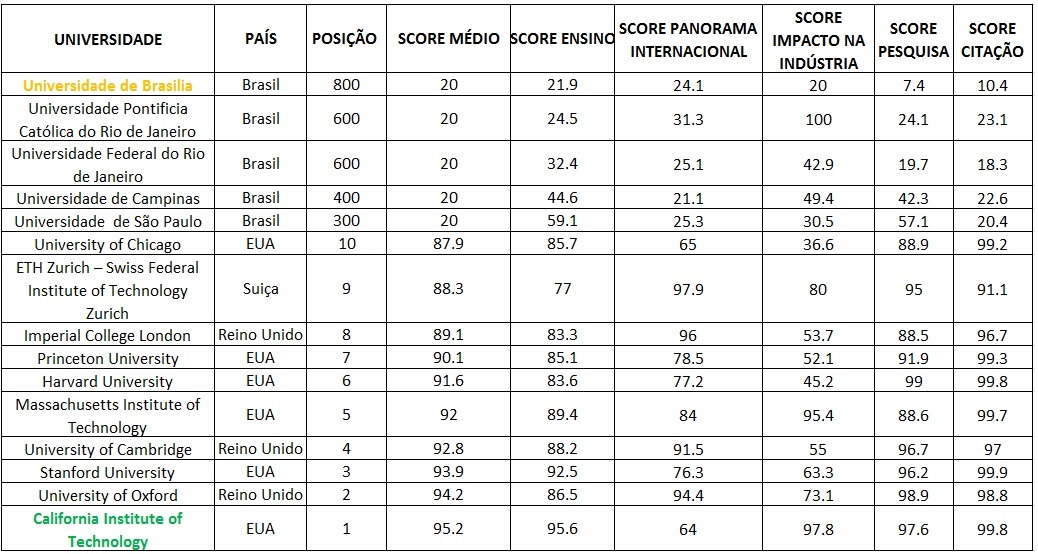
\includegraphics[width=1\textwidth]{figs/tabRankingUniversidades.jpg}
	\caption{Tabela com scores de avalia��o das 5 melhores universidades do mundo e das 5 melhores universidades brasileiras.}
	\label{tabRakingUniversidades}
\end{table}

Pesquisou-se o curr�culo da UnB e o curr�culo da universidade \textit{California Institute of Tecnology} para disciplinas com ementa similar ao de \textit{Algoritmos e Programa��o de Computadores}. O resultado de tal pesquisa � mostrado na tabela \ref{tabRakingUniversidades2}. 

Fez, tamb�m, uma pesquisa mais aprofundada do conte�do program�tico de tais disciplinas. O resultado de tal pesquisa � mostrado na tabela \ref{tabRakingUniversidades3}.

\begin{table}[H]
	\centering
	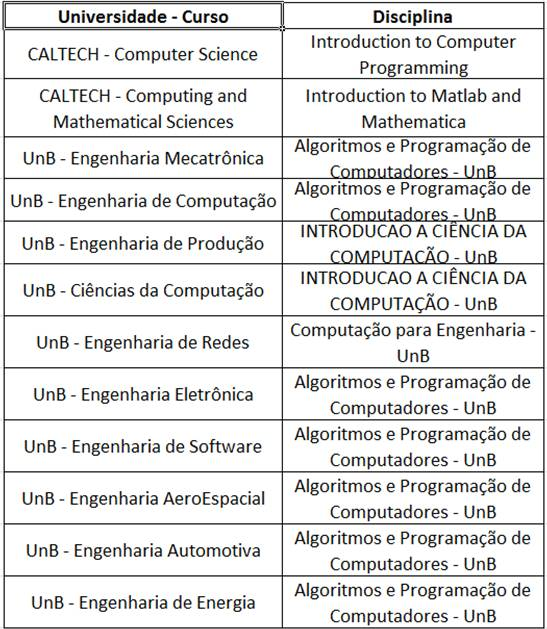
\includegraphics[width=0.7\textwidth]{figs/t2.jpg}
	\caption{Tabela listando as disciplinas na UnB e na \textit{California Insitute of Tecnology} que possuem curr�culo similar a disciplina \textit{Algoritmos e Programa��o de Computadores}.}
	\label{tabRakingUniversidades2}
\end{table}

\begin{table}[H]
	\centering
	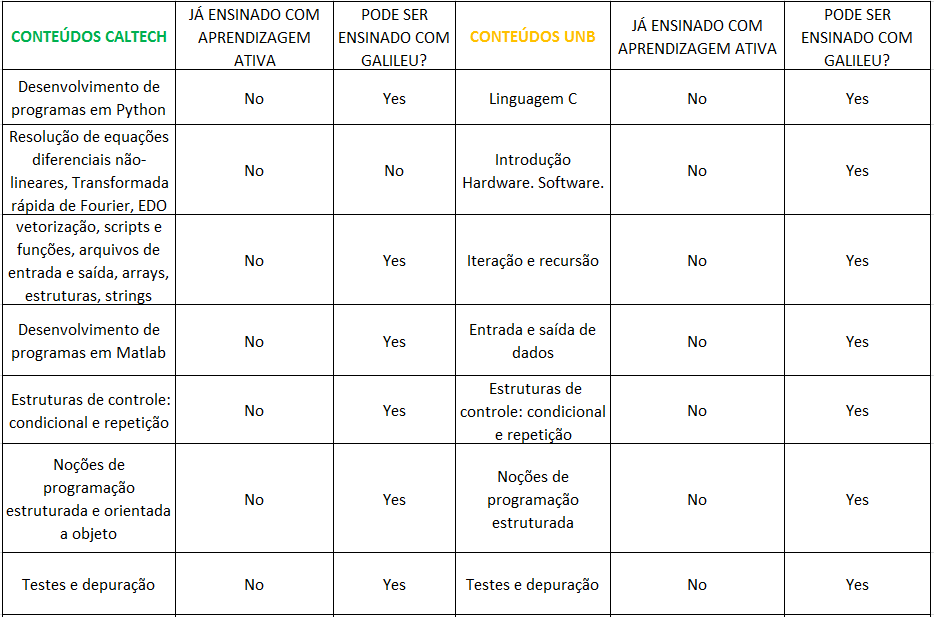
\includegraphics[width=0.7\textwidth]{figs/t3.jpg}
	\caption{Tabela listando parte dos conte�dos tratados pelas disciplinas na \textit{California Insitute of Tecnology} e na UnB e levantanto a quest�o da metodologia de ensino ser uma \textit{metodologia ativa} e se tal conte�do pode ser ensinado usando a placa Galileo.}
	\label{tabRakingUniversidades3}
\end{table}


Para cada conte�do identificado, procurou-se saber tamb�m se ele era tratado de seguindo algum paradigma moderno de \textit{Educa��o Ativa} e, se pela natureza do conte�do, seria poss�vel utilizar a placa Galileo no processo de \textit{ensino-aprendizagem}.

A propor��o de conte�dos que poderiam ser ensinados com a placa Galileo � mostrada na Figura \ref{figPossivelUsarGalileo}.

\begin{figure}[H]
	\centering
	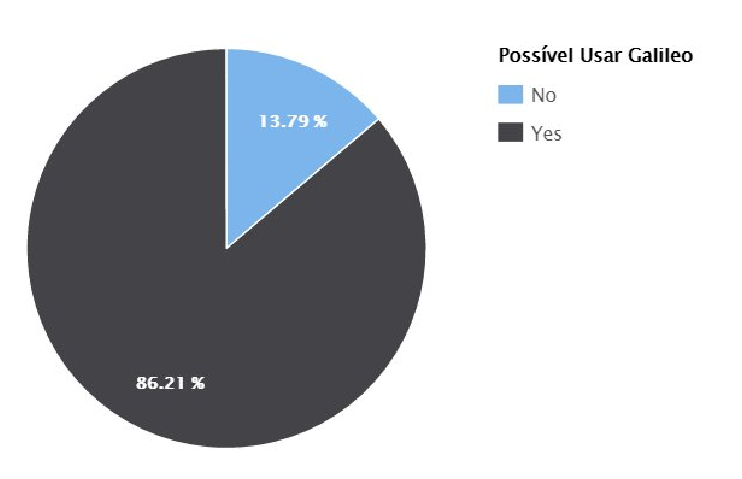
\includegraphics[width=0.7\textwidth]{figs/PossivelUsarGalileo.eps}
	\caption{Percentagem dos conte�dos tratados na UnB e \textit{California Institute of Tecnology} que podem ser ensinados utilizando a placa Galileo.}
	\label{figPossivelUsarGalileo}
\end{figure}

Pode-se concluir, pelas informa��es colhidas nesta se��o, que a mudan�a curr�cular da disciplina \textit{Algoritmos e Programa��o de Computadores} e disciplinas similares em outras faculdades � poss�vel. Tal mudan�a curricular em dire��o � aprendizagem ativa, al�m de trazer grandes benef�cios � qualidade do ensino \cite{Parte1:artigo01}\cite{Parte1:artigo4}, tamb�m pode ajudar a forma��o de novos profissionais alinhados com as compet�ncias mais exigidas no s�culo XXI, como proatividade e independ�ncia \cite{Parte1:artigo1}.


\section{Placa Intel \textsuperscript{\textregistered} Galileo}
\label{CapGalileo}

A placa Intel\textsuperscript{\textregistered}  Galileo � uma \textit{placa de desenvolvimento} com microcontrolador baseado processador Intel\textsuperscript{\textregistered} Quark SoC X1000\cite{DATASHEET0}. A placa Galileo possui software e hardware compat�vel com a placa \textit{Arduino} com rela��o aos pinos digitais e anal�gicos. Um programa escrito para Arduino pode ser usado no Galileu por causa dessa compatibilidade. As Figura \ref{FigPinosFrente} e \ref{FigPinosTras} mostram a placa Intel \textsuperscript{\textregistered} em suas vis�o frontal e traseira. 

Nesta se��o s�o apresentadas, enumeradas e explicadas todas caracter�sticas da placa Intel\textsuperscript{\textregistered} Galileo. 

Primeiramente s�o apresentados os pinos da placa Galileo juntamente com uma breve descri��o de seu uso. Ap�s isso s�o descritas as enumeradas e explicadas todas caracter�sticas eletro-eletr�nicas da placa. Para cada tecnologia na placa � reservada uma pequena sub-se��o neste cap�tulo para sua devida elucida��o.

\begin{comment}
\begin{figure}[tb]
\centering
\mbox{
\subfigure[Placa Intel\textsuperscript{\textregistered} Galileo - Parte Frontal]{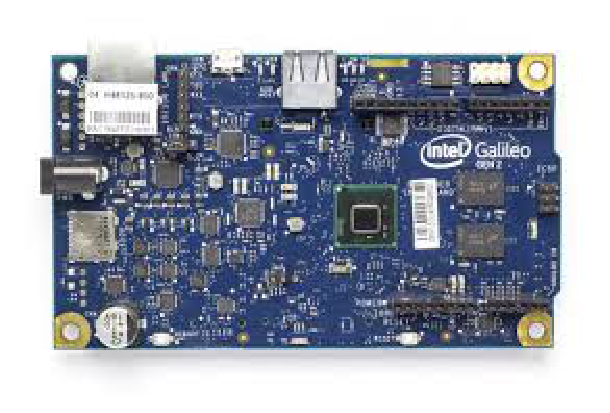
\includegraphics[width=0.3\textwidth]{figs/galileofrente.eps}}\quad\quad
\subfigure[Placa Intel\textsuperscript{\textregistered} Galileo - Parte Traseira]{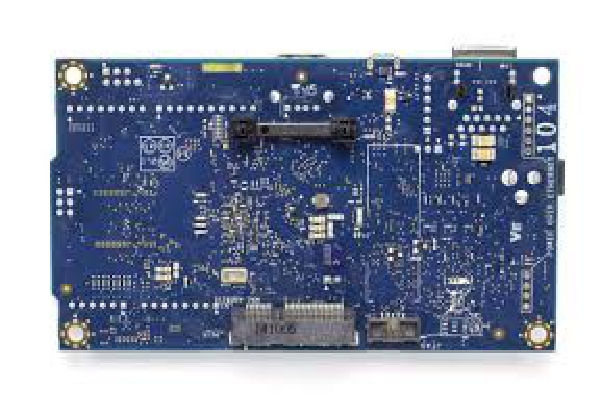
\includegraphics[width=0.35\textwidth]{figs/galileotras.eps}}}

\caption{Placa Intel\textsuperscript{\textregistered} Galileo \cite{DATASHEET1} }
\label{FigPlacaIntelGalileo_vistas}
\end{figure}
\end{comment}

\subsection{Pinagem  da placa Intel \textsuperscript{\textregistered} Galileo}
\label{SecPinagemGalileo}



Os pinos da placa Galileo nas partes frontal e traseira s�o mostrados nas figuras \ref{FigPinosFrente} e \ref{FigPinosTras} 

\begin{figure}[H]
	\centering
	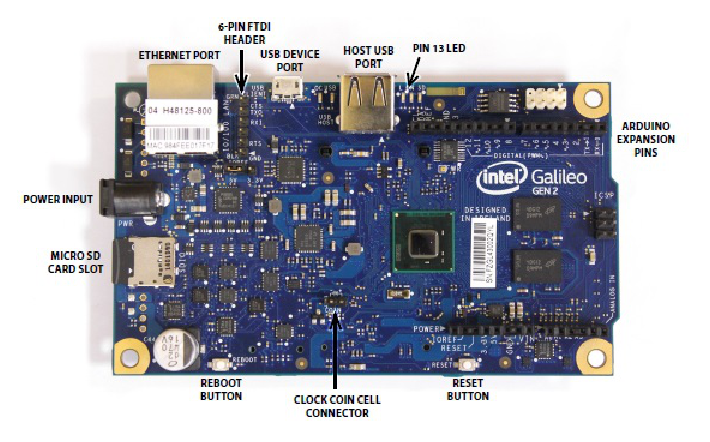
\includegraphics[width=0.31\textwidth]{figs/galileoFrentePinos.eps}
	\caption{Descri��o dos pinos da placa Galileo - parte frontal\cite{DATASHEET1}}
	\label{FigPinosFrente}
\end{figure}


\begin{figure}[t]
	\centering
	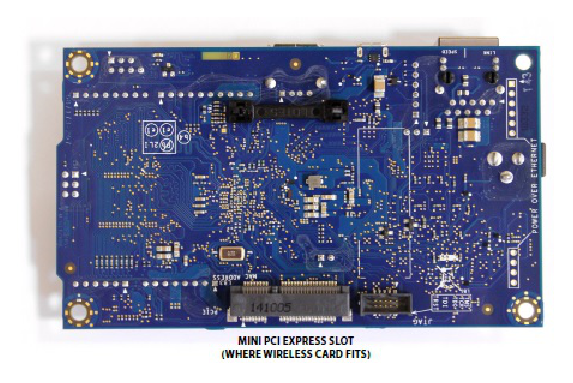
\includegraphics[width=0.31\textwidth]{figs/galileoTrasPinos.eps}
	\caption{Descri��o dos pinos da placa Galileo - parte traseira\cite{DATASHEET1}}
	\label{FigPinosTras}
\end{figure}





A descri��o de cada um desses pinos � a descrita na tabela \ref{TabPinos}:

\begin{table}[]
	\centering
	\caption{Pinos Galileo\cite{DATASHEET1}}
	\label{TabPinos}
	\begin{tabular}{|l|l|}
		\hline
		\textbf{Pino}           & \textbf{Descri��o}                                                                                                                                                                                                 \\ \hline
		Micro SD Card Slot      & \begin{tabular}[c]{@{}l@{}}Pino no qual se pode um SD Card para permitir ao Galileo\\  a execu��o de uma vers�o de Linux com mais recursos\end{tabular}                                                 \\ \hline
		Arduino Expansions Pins & \begin{tabular}[c]{@{}l@{}}Pinos de entrada e sa�da da placa Galileo.\\ Esses pinos s�o compat�veis\\  com os pinos do Arduino e Shields relacionadas.\end{tabular}                                                  \\ \hline
		USB Device Port         & \begin{tabular}[c]{@{}l@{}}Pino para conectar um cabo USB do Galileo ao computador\\  para carregar o Galileo com um programa Arduino\end{tabular}                                                                 \\ \hline
		Host USB Port           & Pino para conectar um dispositivo perif�rico\\ ( como webcam, caixa de som, etc)                                                                                                                                     \\ \hline
		6-Pin FTDI Header       & Adaptador para comunica��o serial computador\\ - Linux instalado no Galileo                                                                                                                                          \\ \hline
		Power Input             & \begin{tabular}[c]{@{}l@{}}Conex�o para bateria de 12V. ATEN��O, a bateria\\ sempre deve ser conectada ao Galileo antes de conectar\\ um cabo USB do Galileo ao computador para evitar\\ danos a placa.\end{tabular} \\ \hline
		Ethernet Port           & Pino para conectar o Galileo � Internet pelo cabo Ethernet                                                                                                                                                         \\ \hline
		Mini PCI Express Slot   & Pino para conectar um cart�o WiFi                                                                                                                                                                                  \\ \hline
		Clock Baterry Power     & \begin{tabular}[c]{@{}l@{}}Conex�o para uma bateria de rel�gio de 3V de forma\\ a fazer com Galileo guarde  informa��es de data e hora\end{tabular}                                                                \\ \hline
		Reboot Button           & Bot�o para realizar a placa, inclusive o sistema operacional                                                                                                                                                       \\ \hline
		Reset Button            & Bot�o para resetar o c�digo que foi carregado no Galileo                                                                                                                                                           \\ \hline
	\end{tabular}
\end{table}



\subsection{Caracter�sticas El�tricas e Eletr�nicas da placa Intel \textsuperscript{\textregistered} Galileo}
\label{CaracteristicasGalileo}
As caracter�sticas el�tricas e eletr�nicas da placa s�o enumeradas a seguir. As caracter�sticas que t�m uma sub-se��o para explica��o mais aprofundada est�o marcadas com \textit{it�lico} e \textbf{negrito}: 
\begin{itemize}
	\item Clock de 400 MHz
	\item Arquitetura Intel\textsuperscript{\textregistered} 32 bits
	\item 14 pinos digitais para entrada e sa�da, 6 das quais podem ser usadas para sa�da \textit{\textbf{PWM}}
	\item 6 pinos para entrada anal�gica utilizando o\textit{\textbf{ conversor anal�gico-digital AD7298}}
	\item Barramento Serial \textit{\textbf{I2C}}
	\item Comunica��o serial com perif�ricos \textit{\textbf{SPI}}
	\item Porta Serial \textit{\textbf{UART}}
	\item 16KBytes de mem�ria \textit{\textbf{L1 Cache}}
	\item 512KBytes de mem�ria \textit{\textbf{SRAM}}
	\item Clock de tempo real integrado \textit{\textbf{(RTC)}}
	\item Barramento \textit{\textbf{PCI Express}}
	\item Conex�o para \textit{\textbf{USB Host e USB Client}}
	\item 10 pinos padr�es \textit{\textbf{JTAG}} para debug
	\item 256 MBytes de mem�ria \textit{\textbf{DRAM}}
	\item 11 KBytes de mem�ria \textit{\textbf{EEPROM}} 
\end{itemize}

\subsubsection{Sinal PWM}
\label{PWM}
Pulse Width Modulation (PWM) ou Modula��o por Largura de Pulso � uma t�cnica que modula��o de impulso utilizada principalmente para codificar uma mensagem num sinal pulsante\cite{livro:Sedra} 

Para o caso do Intel Galileo, as aplica��es do sinal PWM s�o principalmente relacionadas ao controle da tens�o DC fornecida a um circuito. 

O sinal PWM � gerado com ondas quadradas, de p�riodo \textit{T} de ciclo. Durante parte do per�odo, o sinal ter� amplitude \textit{Vmax}. O intervalo de tempo no qual no sinal tem amplitude \textit{Vmax} � chamado \textit{Duty-Cicle} como mostra a Figura \ref{FigPWM}. O valor DC de um sinal peri�dico � calculado como a m�dia aritm�tica da amplitude do sinal no per�odo. O valor da tens�o DC fornecida ao circuito pelo Sinal PWM � calculado com a equa��o \ref{EqPMW1}:     


\begin{figure}[t]
	\centering
	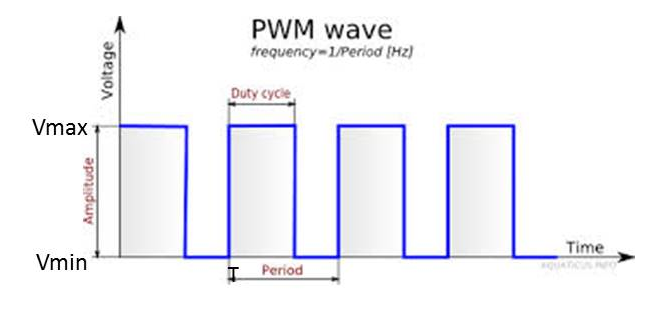
\includegraphics[width=1\textwidth]{figs/PWM.eps}
	\caption{Sinal PWM}
	\label{FigPWM}
	\source{Figura adaptada de http://www.zembedded.com/avr-introduction-to-pwm-part-i/}
\end{figure}    

\begin{equation}
V_{dc} = 1/T() \int_{0}^{Duty Cicle}V_{max} dt + \int_{Duty Cicle}^{T}V_{min} dt%
\label{EqPMW1}
\end{equation}

\begin{equation}
V_{dc} = 1/T(Duty Cicle*V_{max} + T*V_{min} - Duty Cicle*V_{min} )%
\label{EqPMW2}
\end{equation}

Se a tens�o m�nima (Vmin) for igual a zero, o valor DC do sinal PWM � dado por:

\begin{equation}
V_{dc} = \frac{DutyCicle*V_{max}}{T}
\label{EqPMW3}
\end{equation}

A equa��o \ref{EqPMW3} mostra que quanto maior for o tempo que o sinal permanecer no seu valor m�ximo (Vmax), mais pr�ximo de Vmax ser� o valor DC fornecido ao circuito. 

O sinal PMW � gerado na placa Galileo utilizando o clock interno m�ximo de 400 MHz e registradores de Timer espec�ficos para contagem de pulsos do clock. 

Como exemplo para a gera��o do sinal PWM, digamos que o clock da placa foi setado para a frequ�ncia 1kHz. Isso significa que a cada 1ms, o clock gerar� um pulso, como indicado na equa��o \ref{EqPMW4}.

\begin{equation}
f = 1 Khz \;  ->   T = 1ms \; -> 1000\;pulsos\; de\; clock\; por\; segundo
\label{EqPMW4}
\end{equation}

Como a tens�o de opera��o da placa Galileo � 5 V, ent�o:

\begin{equation}
V_{max} = 5 V
\label{EqPMW5}
\end{equation}

Caso se queria gerar um sinal PWM cujo componente DC seja 2.5,  � necess�rio ent�o que durante metade do ciclo do sinal PWM, a amplitude do cinal seja 5 V e durante a outra metade do ciclo, a amplitude seja 0V. Para criar tal sinal, o microcontrolador realiza contagem de pulsos de clock.

Para gerar 2.5 V, o microcontrolador( para a frequ�ncia exemplo de 1kHz) realiza a contagem de 500 pulsos de clock no intervalo de \textit{DutyCicle} e realiza, ap�s isso, a contagem de 500 pulsos no per�odo no qual a amplitude ser� de 0 V.Dessa forma, � gerado digitalmente o sinal PWM na placa Galileo. 

Como dito no �nicio desta se��o, placa Galileo � compat�vel com a placa Ardu�no, tanto a n�vel de hardware quanto a n�vel de software. Da�, para executar a cria��o de um sinal PWM na placa galileu  deve-se chamar a fun��o \textit{analogWrite(int porta, int valor)}. 

A fun��o \textit{analogWrite(int porta, int valor)} recebe como par�metros dois inteiros. O inteiro \textit{porta} indica quais dos pinos digitais, habilitados para sa�da PWM, foi selecionado. O inteiro \textit{valor} deve ser um inteiro entre 0 e 255.
\begin{lstlisting}
//Comando para setar na porta digital 5 o valor 5*(127/255) = 2.5 Volts
analogWrite(5, 127);
\end{lstlisting}

A tens�o DC que estar� presente no pino digital segue a formula: \ref{EqPMW6}

\begin{equation}
V_{dc} =  \frac{5*valor}{255}
\label{EqPMW6}
\end{equation}





\subsubsection{Convers�o anal�gico-digital}
\label{ConversaoAD}
A placa Galileo utiliza para a convers�o anal�gico-digital o circuito integrado \textit{AD7298} \cite{DATASHEET2}. O conversor anal�gico-digital AD7298 � um conversor de 12 bits e usa para a convers�o a t�cnica de \textit{aproxima��es sucessivas}.

A figura \ref{ADC1} mostra uma figura esquem�tica para o processo de convers�o anal�gico-digital utlizando a t�cnica de \textit{aproxima��es sucessivas} e os termos chave para essa t�cnica s�o os seguintes:
\begin{itemize}
	\item Registrador de aproxima��o sucessiva (SAR)
	\item Circuito de amostragem e reten��o ( Track and Hold)
	\item Tens�o de entrada V\textsubscript{IN}
	\item Tens�o de refer�ncia V\textsubscript{REF}
	\item Registrador de N bits (N-BIT REGISTER)
	\item Conversor digital para anal�gico de N bits(N-BIT DAC)
	\item Circuito Comparador
\end{itemize}
Num primeiro instante, o bit mais significante do conversor D/A � setado para 1, enquanto os outros N-1 bits s�o setados para 0. Essa configura��o inicial dos N bits do conversor D/A for�a com que na sa�da exista 1/2 da tens�o de refer�ncia V\textsubscript{REF}, ou seja V\textsubscript{DAC} = 1/2 V\textsubscript{REF}.



\begin{figure}[t]
	\centering
	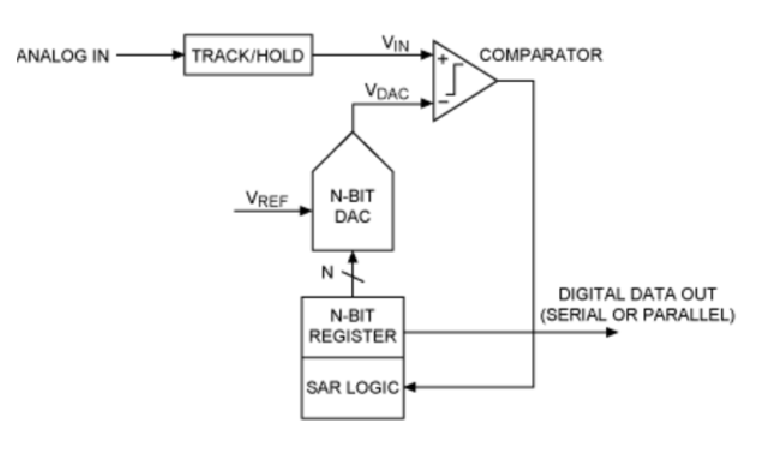
\includegraphics[width=1\textwidth]{figs/ADC1.eps}
	\caption{Figura esquem�tica do processo de convers�o anal�gico para digital}
	\label{ADC1}
	\source{https://www.maximintegrated.com/en/app-notes/index.mvp/id/1080}
\end{figure}
Caso a tens�o V\textsubscript{DAC} seja maior que a tens�o de entrada V\textsubscript{IN}, o bit mais significativo ser� mantido, caso o contr�rio, esse bit ser� setado no valor 0. Depois disso, registrador SAR grava o resultado obtido no comparador no bit avaliado. O processo se repete para os N bits,sempre comparando a tens�o de entrada V\textsubscript{IN} com a tens�o de convers�o V\textsubscript{DAC}, fazendo com que a sa�da da convers�o se aproxime progresivamente a cada itera��o\cite{livroADC}. 

A efici�ncia do processo de convers�o anal�gico-digital est� intimamente ligada ao processo interno de convers�o digital-anal�gico. H� diversos processos de convers�o digital-anal�gico, entretanto, para todos, a quantidade de bits a serem convertidos influencia diretamente na linearidade do processo. Por isso se escolhe, em geral, um conversor digital-anal�gico de 12 bits. 

O conversor A/D utilzado na placa Galileo, segundo seu respectivo datasheet \cite{DATASHEET2}, possui caracter�sticas implementadas que, entre outras incluem:

\begin{itemize}
	\item Sensor de temperatura integrado para devidos ajustes �s varia��es de par�metros causados pela varia��o de temperatura
	\item Taxa de sa�da de convers�es completadas superior a 1 MSPS ( Million Samples Per Second)
\end{itemize}



\subsubsection{Barramento Serial I2C}


I2C(Inter-Intergrated-Circuit) � um protocolo de comunica��o serial desenvolvida originalmente pela \textit{NXP Semiconductor}. Ela permite a comunica��o direta entre diversos componentes utilizando apenas tr�s  barramentos: um barramento para transmiss�o de bits dados - \textit{Serial Data Line(SDA)} - um barramento para o sinal de clock - \textit{Serial Clock Line(SCL)} e um barramento para o uso de um resistor de \textit{pull-up} ligado diretamente uma tens�o V\textsubscript{dd} de 5V ou 3.3V. O endere�amento no protocolo I2C pode ser de 7 ou 10 bits. A velocidade de transmiss�o de dados variam de 10kbits/s - para o modo \textit{low speed}- 400 kbits/s - para o modo \textit{Fast mode} - e 3.4Mbit/s para o \textit{modo Fast mode plus} \cite{livroI2C}. 

O resistor \textit{pull-up} serve para ter como valor alto de tens�o( l�gico 1) tanto o barramento de clock como o barramento de dados, Fig.\ref{I2C1}. Para trocar o valor l�gico enviado nos barramentos, os dispositivos devem chavear suas respectivas conex�es com os barramentos.
\begin{figure}[t]
	\centering
	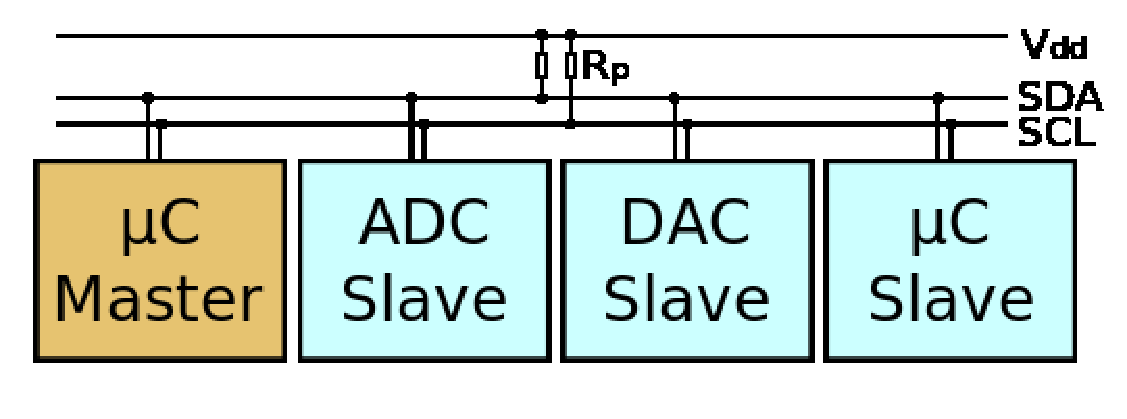
\includegraphics[width=0.8\textwidth]{figs/I2C1.eps}
	\caption{Figura esquem�tica do barramento serial I2C}
	\label{I2C1}
	\source{http://docplayer.com.br/7275040-Monografia-de-graduacao.html}
\end{figure}

No protocolo I2C, sempre existem os dispositivos que agem como \textit{dispositivos mestres}(Masters) e os dispositivos que agem como \textit{dispositivos escravos}(Slaves).

Um \textit{dispositivo mestre} pode escolher com qual dos \textit{dispositivos escravos} ele deseja se comunicar realizando a "mensagem de in�cio".Ap�s isso mandando os bits de endere�o do \textit{dispositivo escravo} s�o enviados no barramento de dados. � enviada, juntamente com uma mensagem do endere�o, uma indica��o, por parte do \textit{dispositivo mestre} mostrando se ele deseja escrever ou ler do \textit{dispositivo escravo}. Ap�s isso, o \textit{dispositivo escravo} deve enviar uma mensagem ACK para completar o estabelecimento da comunica��o.Para enviar uma mensagem ACK, o \textit{dispositivo escravo} seta o barramento de dados para o valor 0.   

Tendo sido estabelecida a comunica��o entre \textit{dispositivo mestre} e \textit{dispositivo escravo}, � incub�ncia do \textit{dispositivo escravo} enviar, a cada 8 bits recebidos, uma mensagem ACK. 


Os \textit{dispositivos mestres} sempre retem o controle do barramento de clock. Quando um \textit{dispositivo mestre} faz com que o barramento de clock tenha o valor l�gico 0, � indicado para os \textit{dispositivos escravos} que eles devem setar o barramento de dados com um bit 0 ou 1.
\begin{figure}[H]
	\centering
	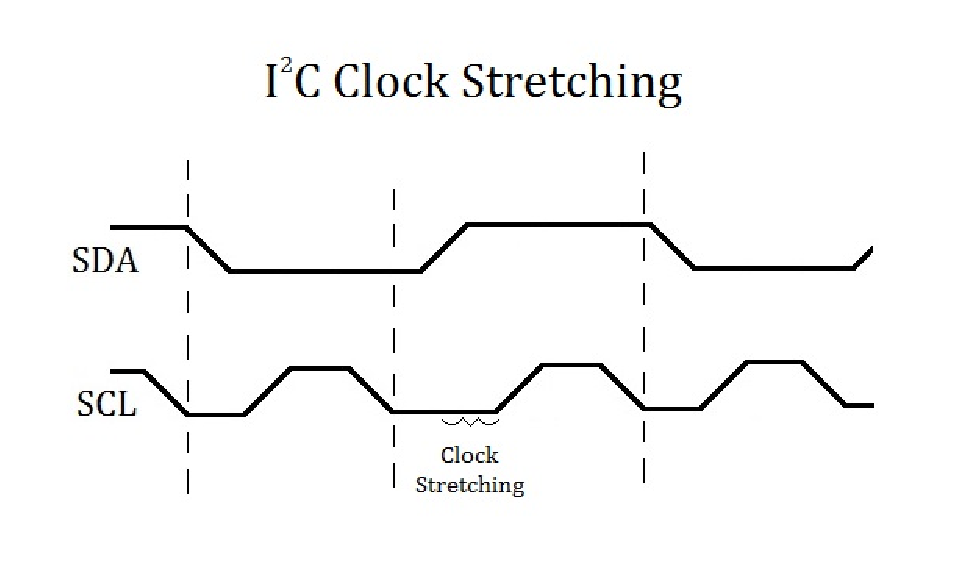
\includegraphics[width=0.6\textwidth]{figs/I2C2.eps}
	\caption{I2C - Clock Stretching }
	\label{I2C2}
	\source{https://blog.digilentinc.com/index.php/i2c-how-does-it-work/}
\end{figure}

Para assegurar o recebimento dos dados, os \textit{dispositivo escravos} podem, possivelmente, realizar o chamado \textit{Clock Stretching},, Fig \ref{I2C2}, o qual consiste em manter o barramento de clock no n�vel 0, mesmo que o mestre o tenha setado para o n�vel. Isso � feito para, ampliar o tempo do processo de recebimento dos dados, por parte dos \textit{dispositivo escravos}, para assegurar o sucesso de tal processo.

I2C oferece um bom suporte para a comunica��o entre dispositivos eletr�nicos  que s�o acessados de forma ocasional. A vantagem competitiva da I2C sobre outros protocolos de comunica��o de curta dist�ncia de baixa velocidade � que seu custo e complexidade n�o aumenta com o n�mero de dispositivos no barramento. 

Por outro lado, a complexidade dos componentes de software I2C de suporte pode ser significativamente mais elevada do que a de v�rios protocolos concorrentes (SPI e MicroWire, por exemplo) com uma configura��o muito simples. Entretanto, seu modelo de endere�amento pr�prio, aliado com a forma de transfer�ncia simples de bytes para necessidades de comunica��o simples.

O protocolo I2C � muito utilizado em projetos no placas Galileo utilizando a biblioteca: \textit{Wire.h}




\subsubsection{Comunica��o serial SPI}

Assim como o protocolo I2C, o protocolo de Interface Serial com Perif�ricos - Serial Peripheral Interface (SPI) - tem como utilidade a comunica��o de curta dist�ncia entre dispositivos eletr�nicos\cite{LivroSPI}.

No protocolo SPI, h� apenas um \textit{dispositivo mestre} para v�rios \textit{dispositivo escravos}. A comuninca��o entre os \textit{dispositivo mestre} e os \textit{dispositivos escravos} � \textit{full-duplex}, ou seja, os dispositivos citados podem se comunicar entre si em ambas dire��es. Os pinos \textit{dispositivo mestre} e nos \textit{dispositivos escravos}, como mostrados na Figura \ref{SPI1}, s�o os seguintes:

\begin{itemize}
	\item SCLK: Barramento Serial para o sinal de Clock originado no \textit{dispositivo mestre}
	\item MOSI: \textit{Master Output Slave Input}; sinal originado no \textit{dispositivo mestre}
	\item MISO: \textit{Master Input Slave Output};sinal originado em um dos \textit{dispositivos escravos}
	\item SS: \textit{Slave Select}; sinal originado no \textit{dispositivo mestre}
	
\end{itemize}


\begin{figure}[t]
	\centering
	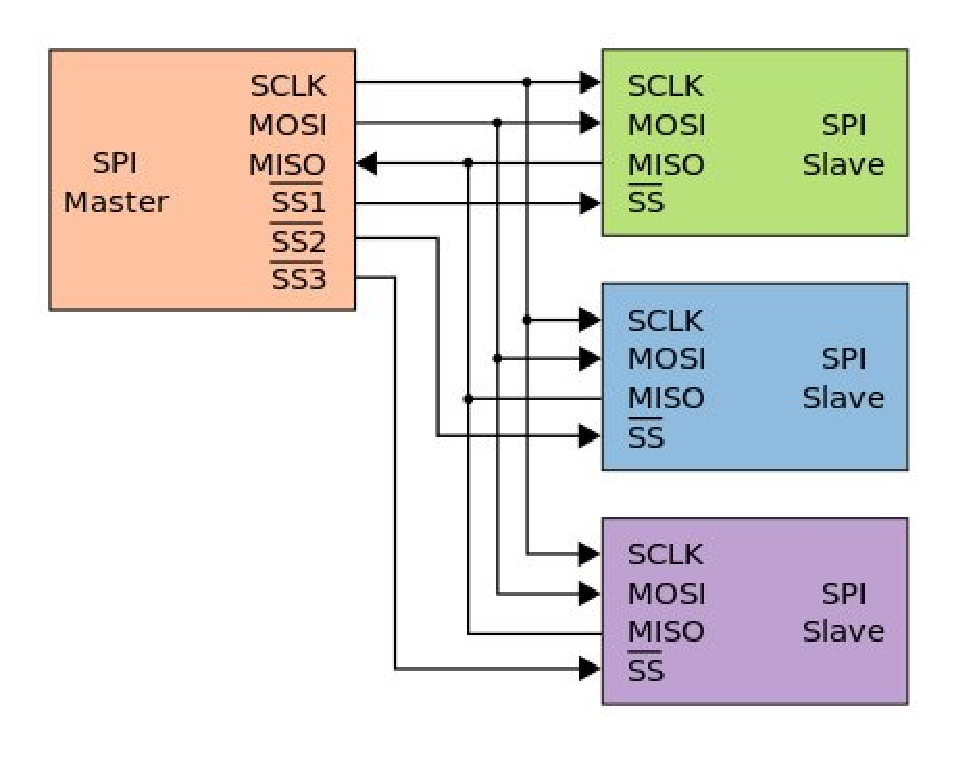
\includegraphics[width=0.8\textwidth]{figs/SPI0.eps}
	\caption{Barramento SPI - Um \textit{dispositivo mestre} para \textit{dispositivos escravos}  }
	\label{SPI1}
	\source{http://docplayer.com.br/3514866-Pratica-8-comunicacao-spi-8-1-introducao-e-objetivos-8-2-principios-basicos-do-protocolo-spi.html}
\end{figure}

O pino SS � utilizado pelo \textit{dispositivo mestre} para selecionar com qual dos \textit{dispositivos escravos} ele se comunicar� (seja para receber mensagens ou enviar). Usualmente, quando um dos \textit{dispositivos escravos} � selecionado, todos outros, pela l�gica \textit{tri-state} das entradas SS, assumem altas imped�ncia de entrada - o que significa que virtualmente tais escravos est�o desconectados do circuito com o \textit{dispositivo mestre}.

Primeiramente, no come�o da comunica��o com o dispositivo selecionado, � configurado no \textit{dispositivo mestre} a frequ�ncia do clock que sai da pino SCLK.

Ap�s isso, come�a a ocorrer a troca de bits entre os dispositivos. Para cada bit que o pino MOSI recebe, � tamb�m recebido um bit no pino MISO. 

Comparado a outros protocolos de inter-comunica��o, o protocolo SPI oferece uma das maiores taxas de sa�da de bits. Isso se deve, dentre outros fatores, a n�o limita��o do tamanho da palavra bin�ria transmitida. As taxas de transmiss�o s�o, em geral, da ordem de MHz, entretanto tal taxa � intimamente ligada a velocidade do clock no \textit{dispositivo mestre}, podendo portanto ser livremente aumentada. Al�m disso, os \textit{dispositivos escravos} n�o necessitam de um endere�o �nico como no protocolo I2C, da�, todas fase de reconhecimento e estabelecimento de comunica��o � facilitada. Entretanto, tais facilidades tornam o protocolo com dificil debura��o de erros e n�o h� controle de fluxo nem nos \textit{dispositivos escravos}.

SPI � utilizado em muitas aplica��es. Dentre elas, por exemplo:
\begin{itemize}
	\item Aplica��es com sensores:
	\begin{itemize}
		\item Comunica��o com sensores de temperatura
		\item Comunica��o com sensores de press�o
		\item Comunica��o com sensores de toque
	\end{itemize}
	\item aplica��es com tipos espec�ficos de m�moria
	\begin{itemize}
		\item Flash
		\item EEPROM
	\end{itemize}
	
\end{itemize}

Para fazer projetos com SPI na placa Galileo deve ser utilizada a biblioteca \textit{SPI.h}

\subsubsection{Porta Serial UART}

UART significa \textit{Universal Asynchronous Receiver/Transmitter} (Receptor/Transmissor Universal Ass�ncrono). Um dispositivo UART � um microchip que tem como responsabilidade controlar a comunica��o de um computador ou microcontrolador conectados serialmente. Essencialmente, um dispositivo UART � a dispositivo intermedi�rio entre interfaces seriais e paralelas\cite{LivroUART}.

\begin{figure}[t]
	\centering
	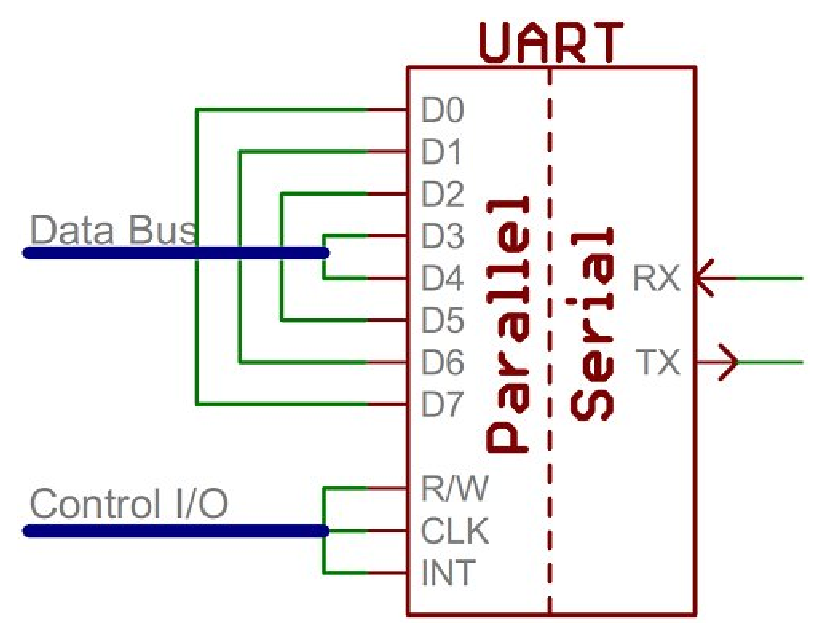
\includegraphics[width=0.7\textwidth]{figs/UART2.eps}
	\caption{Modelo simplificado de um dispositivo UART}
	\label{UART2}
	\source{https://learn.sparkfun.com/tutorials/serial-communication/uarts}
\end{figure}

A Figura \ref{UART2} mostra um modelo simplicado do que consiste um dispositivo UART. Na parte esquerda da figura, s�o mostrados os pinos de comunica��o paralela pelo barramento de dados (Data Bus). O pinos R/W � utilizado para setar entre modos de leitura e escrita (Read/Write). O pino CLK � o pino do sinal de clock. O pino INT � o pino usado para interrup��o de software para avisar o sistema que h� dados para serem lidos/escritos no dispositivo UART.
\begin{figure}[t]
	\centering
	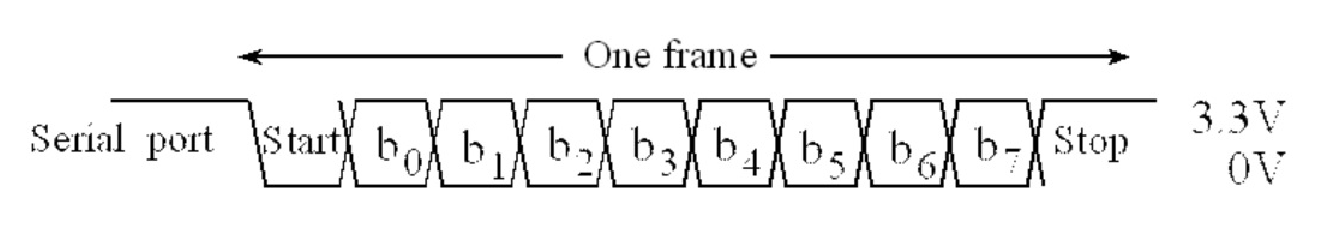
\includegraphics[width=0.8\textwidth]{figs/UART1.eps}
	\caption{Frame UART para transmiss�o de 1 byte }
	\label{UART1}
	\source{http://www.mathworks.com/help/hdlverifier/examples/generate-fifo-interface-dpi-component-for-uart-receiver.html?requestedDomain=www.mathworks.com}
\end{figure}

A Figura \ref{UART1} mostra o chamado \textit{frame} de dados da placa UART. O \textit{frame} � composto de 10 bits. O primeiro bit � o bit de \textit{start} utilizado para indicar o �nicio do envio ou recebimento de um byte (8 bits) de dados. O bit \textit{stop} indica o fim do frame. 
\begin{figure}[t]
	\centering
	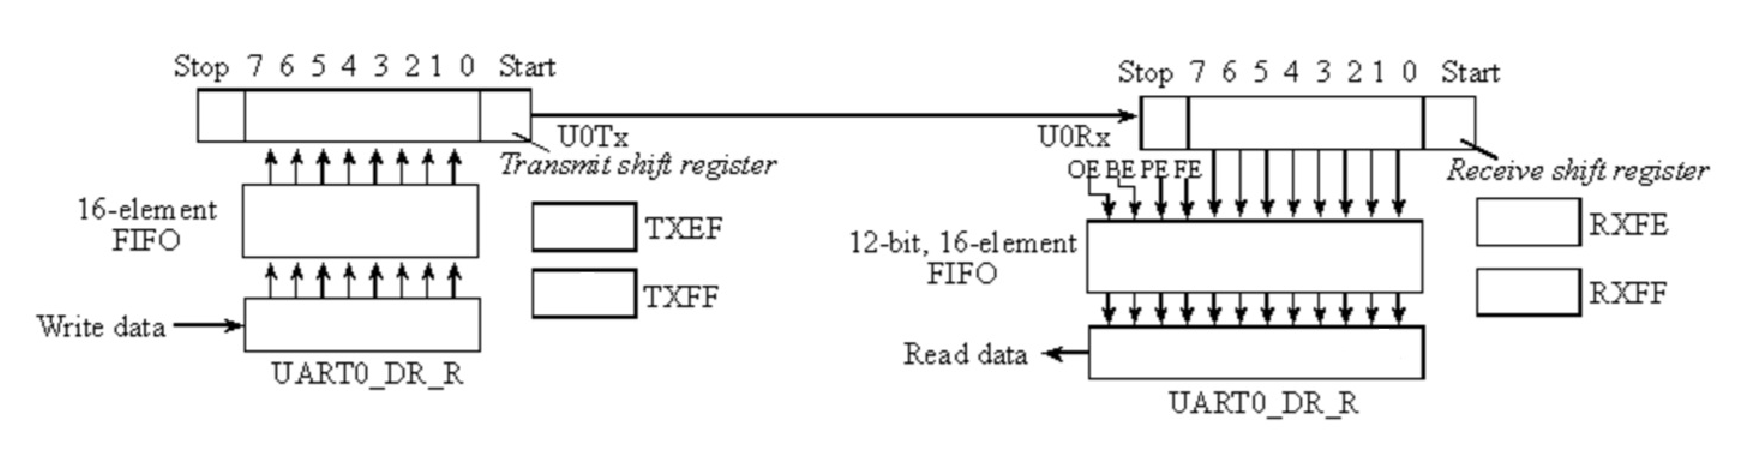
\includegraphics[width=1\textwidth]{figs/UART3.eps}
	\caption{Modelo completo de um dispositivo UART}
	\label{UART3}
	\source{http://users.ece.utexas.edu/valvano/Volume1/E-Book/C11\_SerialInterface}
	
\end{figure}

J� a Figura \ref{UART3} mostra em detalhes o processo que ocorre num dispositivo UART. Na figura, \verb|UART_DR_D| � o \textit{registrador de dados (Data Register)}, o qual � preenchido pela dispositivo que deseja realizar a comunica��o utilizando o dispositivo UART. FIFO � a fila de recebimento(RX) ou transmiss�o de dados(TX). Ambas as filas tem 16 bits de tamanho. No caso da fila de recebimento de dados, 4 dos 16 bits s�o bits de flags para indicar erros na transmiss�o.

RXFE � uma flag que indica se que a fila de recebimento  est� vazia e RXFF � outra flag que indica que a fila de recebeminto est� vazia. Quanto as filas de transmiss�o, TXEF indica que a fila est� vazia e TXFF indica que a fila est� cheia. UOTX e UORX s�o \textit{shift register} s�o os respons�veis pela transforma��o da comunica��o em s�rie para paralela e vice-versa. 

O processo de transmiss�o de dados � o seguinte:

\begin{itemize}
	\item 1) Dados armazenados no registrador de dados s�o enviados para a fila
	\item Caso a fila esteja vazia( flag TX), a fila recebe os bits do registrador de dados
	\item 2) Os bits s�o enviados para o shift register UOTX, come�ando no b0 e sendo "shiftados" at� o bit b7.
	\item 3) Os bits armazenados no UOTX s�o enviados de forma serial para 
	o shift register receptor UORX.
	\item 4) Caso a fila de recep��o esteja vazia (flag RX), os dados s�o colocados na pilha e l� permanecem at� serem lidos.
\end{itemize} 

UART � muito utilizado para projetos que requerem comunica��o serial com Galileo ou projeto de Multiplas Entradas e Sa�da �nica (MISO) ou projeto com Entrada �nica e Sa�da M�ltipla (SIMO). Para trabalhar com UART, deve usar a biblioteca \textit{SoftwareSerial.h}


%%SPI
%? EEPROM
%? UART
%? GPIO
%? Wi-Fi
%? Servo
%? USB Host 

\subsubsection{Mem�ria Cache}

Dentre as opera��es num sistema computacional, a opera��o mais demorada � o acesso � mem�ria. Para evitar tais opera��es, � usada a chamada mem�ria cache\cite{LivroCache}. 

A mem�ria cache faz parte da organiza��o da mem�ria de um sistema computacional. A mem�ria num sistema computacional � organizada da seguinte forma, Fig.\ref{CACHE0}:
\begin{itemize}
	\item Mem�ria de armazenamento(Storage Device - Mem�ria ROM): Este n�vel de mem�ria � o que poss�vel mais espa�o, entretanto � a mem�ria que demanda mais tempo para ser modificada, por isso, em geral, nesse n�vel ficam armazenados sistemas operacionais, arquivos de BOOT do sistema, firwares, etc. A mem�ria nesse n�vel n�o-vol�til, o que significa que ela n�o � perdida ao se desligar o sistema.
	\item RAM(Random Access Memory): Este n�vel de mem�ria � utilizado como mem�ria principal. A mem�ria RAM � de leitura e escrita. Essa mem�ria � utilizada pelo CPU para armazenar e ler dados, arquivos e programas que est�o sendo utilizados no momento. A mem�ria RAM � uma mem�ria vol�til, o que significa que o conte�do armazenado nela � perdido ap�s o desligamento do sistema.
	\item A mem�ria cache � a parte da mem�ria utilizada pela unidade de processamento central (CPU) de um computador para reduzir o tempo m�dio necess�rio para ler ou escrever aos dados a partir da mem�ria principal. A mem�ria cache � uma mem�ria menor, mais r�pida que armazena c�pias dos dados de localiza��es de mem�ria principais utilizados com frequ�ncia para evitar a repeti��o de acessos lentos. A maioria dos processadores t�m diferentes caches independentes, incluindo instru��es e dados caches, onde o cache de dados � normalmente organizadas como uma hierarquia de n�veis mais cache (L1, L2, etc).
	\item CPU: Na CPU est� armazenada toda arquitetura de instru��es do sistema computacional. A CPU � respons�vel pela ger�ncia de todos processos que ocorrem no computador e ela utiliza a mem�ria cache para realizar a maior parte de suas opera��es
	
\end{itemize}

Para toda opera��o que a CPU executa a qual necessita de certo dado da mem�ria, � sempre verificadp, primeiramente, se o dado j� se encontra na mem�ria cache. Caso o dado n�o se encontre na cache, � solicitado dos n�veis mais baixos da mem�ria o dado em quest�o. Caso o dado j� se encontre na cache, ele � lido e processado rapidamente pela CPU.

Microcontroladores simples, em geral, n�o possuem a mem�ria cache, visto que toda sua estrutura � simplificada. No caso da placa Galileo e placas similares, a mem�ria cache � necess�ria, visto que tais sistemas podem, inclusive, executar sistemas operacionais e tem grande quantidade de mem�ria de armazenamento.

Atualmente, vem-se dividindo a m�moria cache em n�veis: cache L1, cache L2, cache L3, etc. Tal divis�o � feita para amplificar o efeito de manter na cache os dados de mem�ria usualmente acessados. A cache L1 cont�m os dados acessados mais frequentemente, a cache L2 cont�m os dados acessados frequentemente, mas n�o tanto quanto os dados na cache L1, etc. 

No caso da placa Galileo, h� apenas um n�vel de cache: a cache L1 com 16 KBytes, como mostrado na se��o \ref{CaracteristicasGalileo}.

\begin{figure}[t]
	\centering
	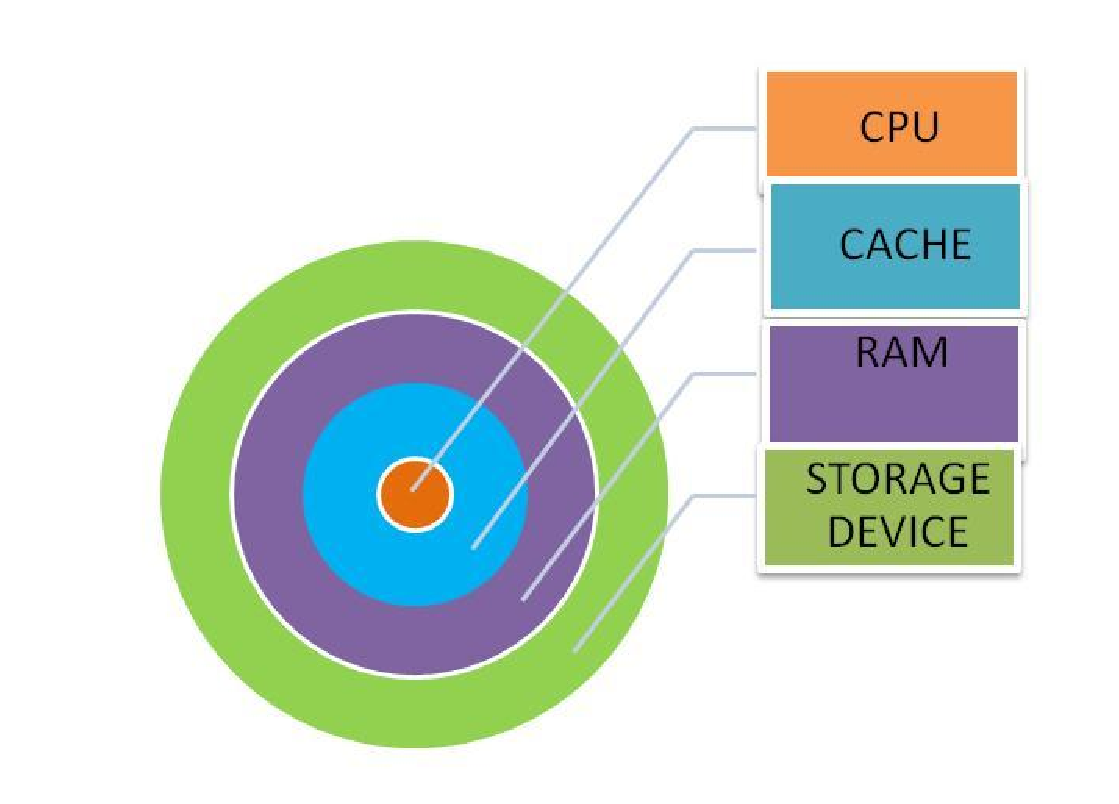
\includegraphics[width=0.5\textwidth]{figs/cache0.eps}
	\caption{Organiza��o da mem�ria num sistema computacional}
	\label{CACHE0}
\end{figure}


\subsubsection{Mem�ria SRAM}

Mem�ria SRAM (Static Random Access Memory) � o tipo de mem�ria de acesso aleat�rio geralmente utilizado no n�vel de mem�ria cache. Ser de de acesso aleat�rio significa que qualquer por��o da mem�ria � acessada num tempo igual. SRAM � uma mem�ria est�tica, o que significa que o dados se manter� armazenado durante um largo intervalo de tempo depois do desligamento do sistema.

A mem�ria SRAM � constru�da utilizando com flip-flops com transistores MOSFETs. A Figura \ref{SRAM0} mostra a estrutura b�sica de armazenamento de uma c�lula de um bit da mem�ria SRAM. 
\begin{figure}[t]
	\centering
	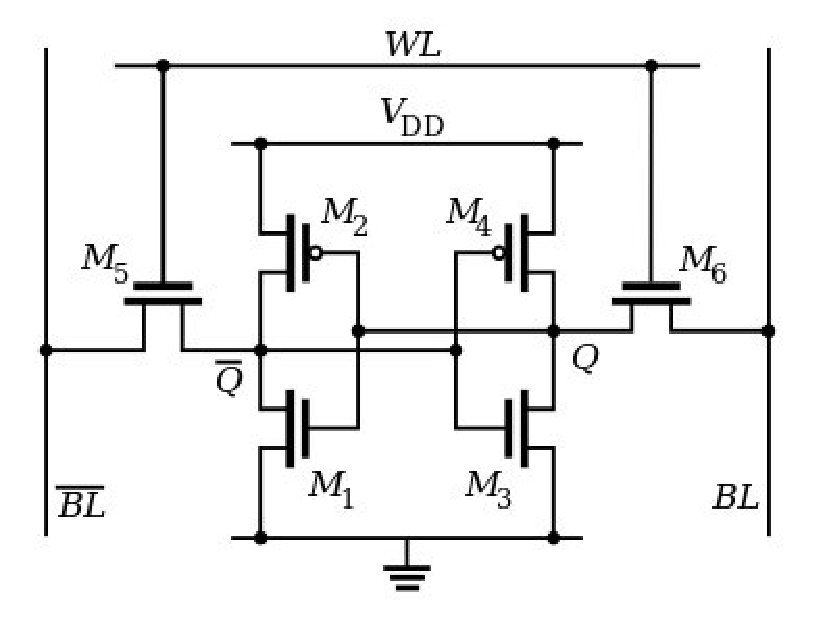
\includegraphics[width=0.4\textwidth]{figs/SRAM0.eps}
	\caption{Estrutura da c�lula de mem�ria SRAM}
	\label{SRAM0}
	\source{http://web.sfc.keio.ac.jp/~rdv/keio/sfc/teaching/architecture/architecture-2009/lec08-cache.html}
\end{figure}

Resumidamente, os transistores M1, M2, M3 e M4 s�o os respons�veis por guardar o bit\cite{LivroSRAM}. A estrutura do circuito formada por M1, M2, M3 e M4 realiza a realimenta��o do bit, sendo respons�vel pelo qualidade de mem�ria est�tica que a SRAM possui. A Figura \ref{SRAM1} mostra como os transistores M1, M2, M3 e M4 podem ser vistos como um par de emissores. Quando um Q, na Figura \ref{SRAM1}, � igual a 1, seu oposto, $\overline{Q}$ = 0, � criado na saida do inverso e o sinal Q = 1 � realimentado pelo segundo inversor. 

\begin{figure}[t]
	\centering
	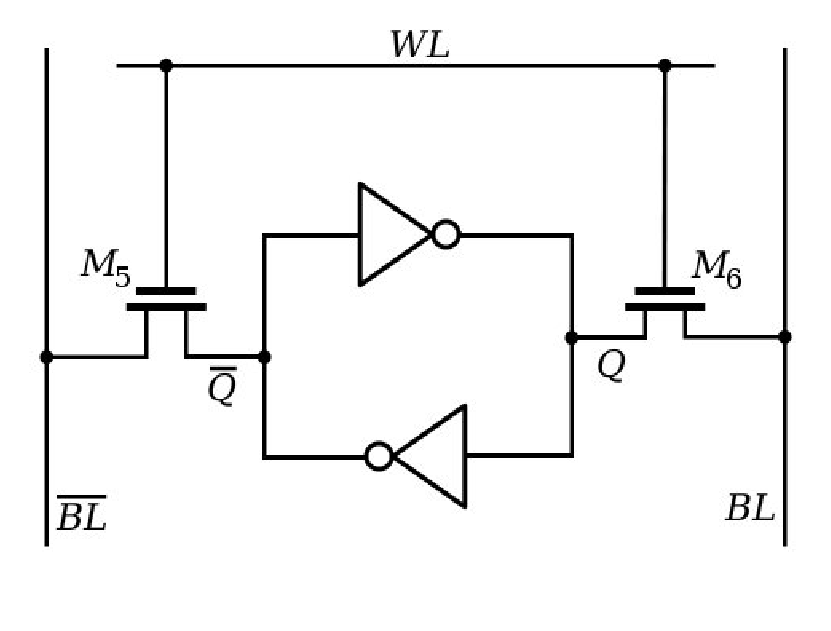
\includegraphics[width=0.4\textwidth]{figs/SRAM1.eps}
	\caption{Estrutura da c�lula SRAM com dois inversores}
	\label{SRAM1}
	\source{http://web.sfc.keio.ac.jp/~rdv/keio/sfc/teaching/architecture/architecture-2009/lec08-cache.html}
\end{figure}


Dessa maneira, a estrutura da c�lula de um bit de mem�ria SRAM torna desnecess�rio \textit{recarregamento} do dado armazenado. Os transistores M5 e M6 s�o usados para ler ou escrever da c�lula de mem�ria por meio das linhas de bit BL e $\overline{BL}$. Tal processo de leitura ou escrita pode ser realizado, em m�dia, em 2ns, velocidade a qual � bastante alta para sistemas computacionais.

A mem�ria SRAM � utilizada n�s mais variados ambientes como: computadores pessoais, microcontroladores, FPGAs, etc. Na placa Galileo, existem 512 Kbytes de SRAM integrados, tornando a placa Galileo altamente eficiente no tocante ao acesso e atualiza��o da mem�ria.  

\subsubsection{Mem�ria DRAM}

Dynamic Random Access Memory (DRAM) � uma mem�ria de acesso aleat�rio como a SRAM. Ao contr�rio da mem�ria SRAM, a mem�ria DRAM � uma mem�ria \textit{din�mica}, o que significa que os dados armazenados precisam ser periodicamente recarregados.

\begin{figure}[t]
	\centering
	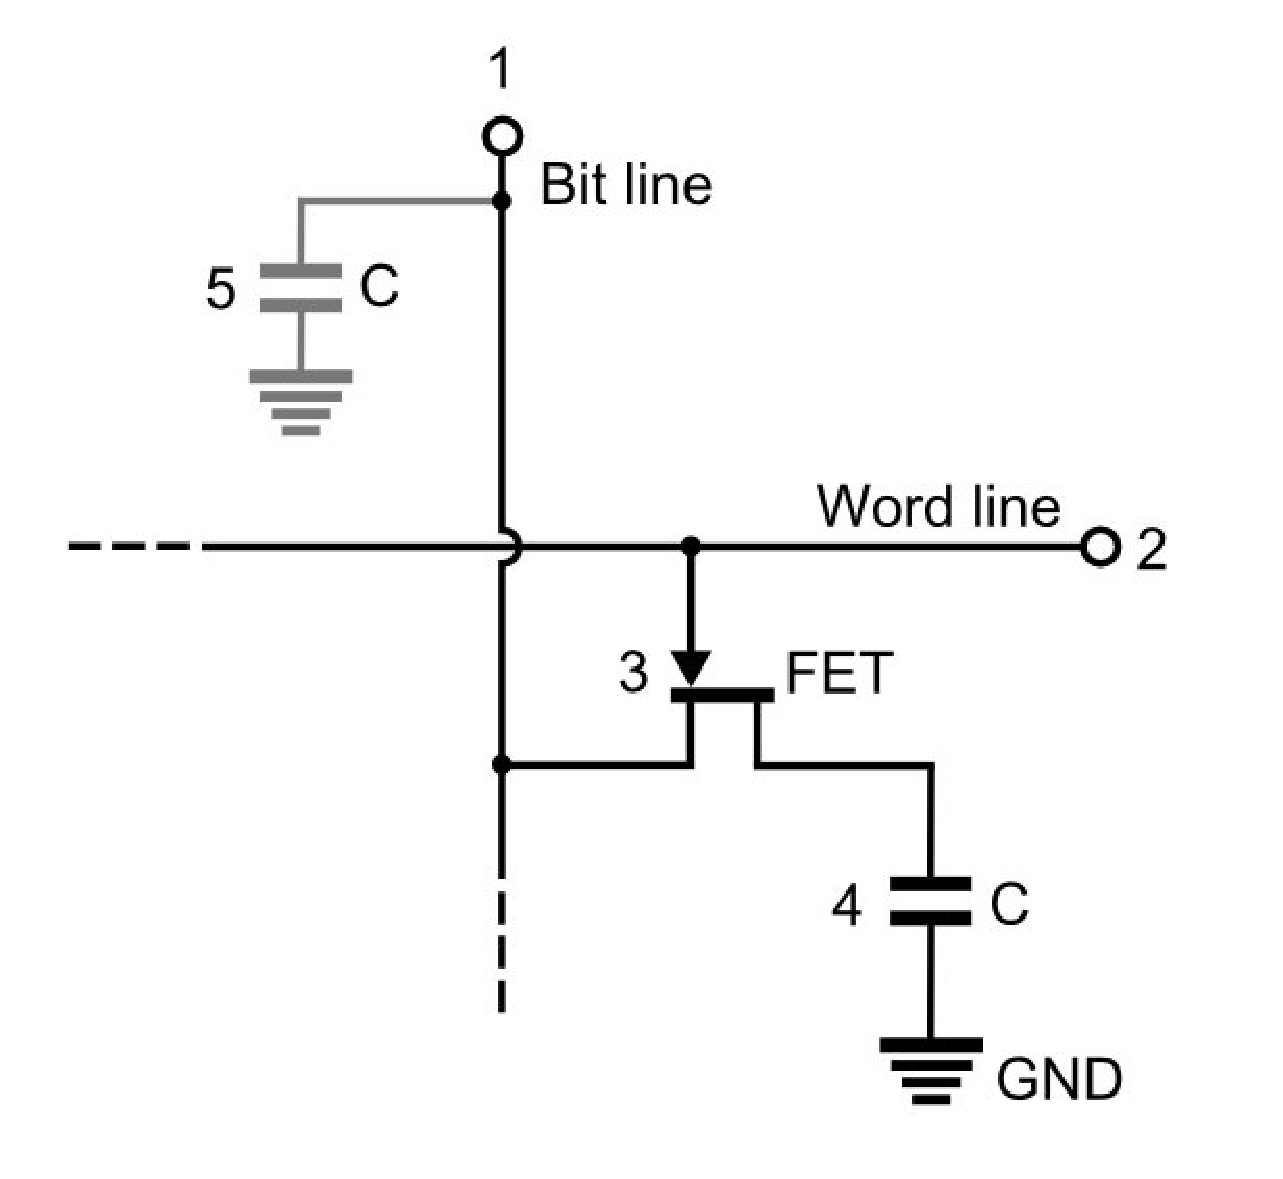
\includegraphics[width=0.7\textwidth]{figs/DRAM1.eps}
	\caption{Estrutura da c�lula de mem�ria DRAM}
	\label{DRAM1}
	\source{http://users.ece.gatech.edu/~sudha/academic/class/ece2030/Lectures/memory/}
\end{figure}



Os bits, na m�moria DRAM, s�o armazenados numa estrutura de um capacitor juntamente com um transistor. O capacitor estar carregado significa o bit 1, e o capacitor est� descarregado significa o bit 0. Na Figura \ref{DRAM1} � mostrada a estrutura de uma c�lula de mem�ria DRAM. O capacitor marcado pelo n�mero 4 � onde o bit � armazenado.

O processo de escrita no bit � da seguinte forma:

\begin{itemize}
	\item 1) Na linha marcada pelo n�mero 1(Bit Line) � escrito um bit l�gico 0 ou 1( 0 ou +Vcc Volts)
	\item 2) A linha marcada pelo n�mero 2 ativa o transistor conectando a Bit line com o capacitor C (marcado pelo n�mero 4) 
\end{itemize}

O processo de leitura � feita da mesma forma que o processo de escrita, entretanto, a Bit line possui capacit�ncia parasita apreci�vel. Na figura, essa capacit�ncia � marcada pelo n�mero 5. Tal capacit�ncia parasita diminui a velocidade do processo de leitura por tomar parte da carga armazenada no capacitor marcado pelo n�mero 4 para si.

O descarregamento natural dos capacitores, ainda que em circuito aberto, e a exist�ncia de capacitores parasitas na c�lula de mem�ria trazem a necessidade de circuitos respons�veis por recarregar, a cada leitura, as c�lulas DRAM.

O tempo m�dio de leitura na mem�ria DRAM � de 64 ns. Pelo tempo de leitura e pela necessidade de recarregamento, em geral, a mem�ria DRAM � usada para mem�rias menos acessadas. 

A placa Galileo possui 256 MByte de mem�ria DRAM gerenciados pelo sistema operacional.


\subsubsection{Mem�ria EEPROM}

EEPROM, Electrically Erasable Programmable Read-Only Memory � uma mem�ria n�o vol�til, o que significa que os dados n�o s�o apagados ap�s o desligamento do sistema. A mem�ria EEPROM � similar � mem�ria FLASH. Assim como ela, a mem�ria EEPROM escrita aproximadamente 100.000 vezes. A principal vantagem que a mem�ria EEPROM apresenta em rela��o a mem�ria FLASH � que ela deve escrever em bytes individualmente, enquanto na mem�ria FLASH � necess�rio escrever um setor inteiro para alterar bytes individuais. Tal caracter�stica torna a mem�ria FLASH mais r�pida e com vida-�til menor que a mem�ria EEPROM.

Na placa Galileo h� 11 Kbytes mem�ria EEPROM. A EEPROM pode ser programada na placa Galileo com a biblioteca \textit{EEPROM.h}.

\subsubsection{Clock de tempo real - RTC}

Um clock de tempo (RTC) � um clock comum de um sistema computacional com a funcionalidade de ter armazenado nele tempo atual, mesmo que o sistema esteja desligado. Quase todos equipamentos eletr�nicos atuais, como computadores, celulares, etc, possuem um clock de tempo real integrado. O tempo atual pode ser adquirido com outros equipamentos al�m do RTC, entretanto, o RTC t�m as seguintes vantagens:

\begin{itemize}
	\item Baixo consumo de energia
	\item O fato de ser um sistema indepedente do sistema central, faz com este tenha seu processamento livre para outras tarefas
\end{itemize}


\subsubsection{Barramento Mini PCI-Express}

Mini PCI-Express � um barramento de alta velocidade de transmiss�o de dados com 52 pinos. Por meio desses 52 pinos, existem as seguintes conex�es:

\begin{figure}[t]
	\centering
	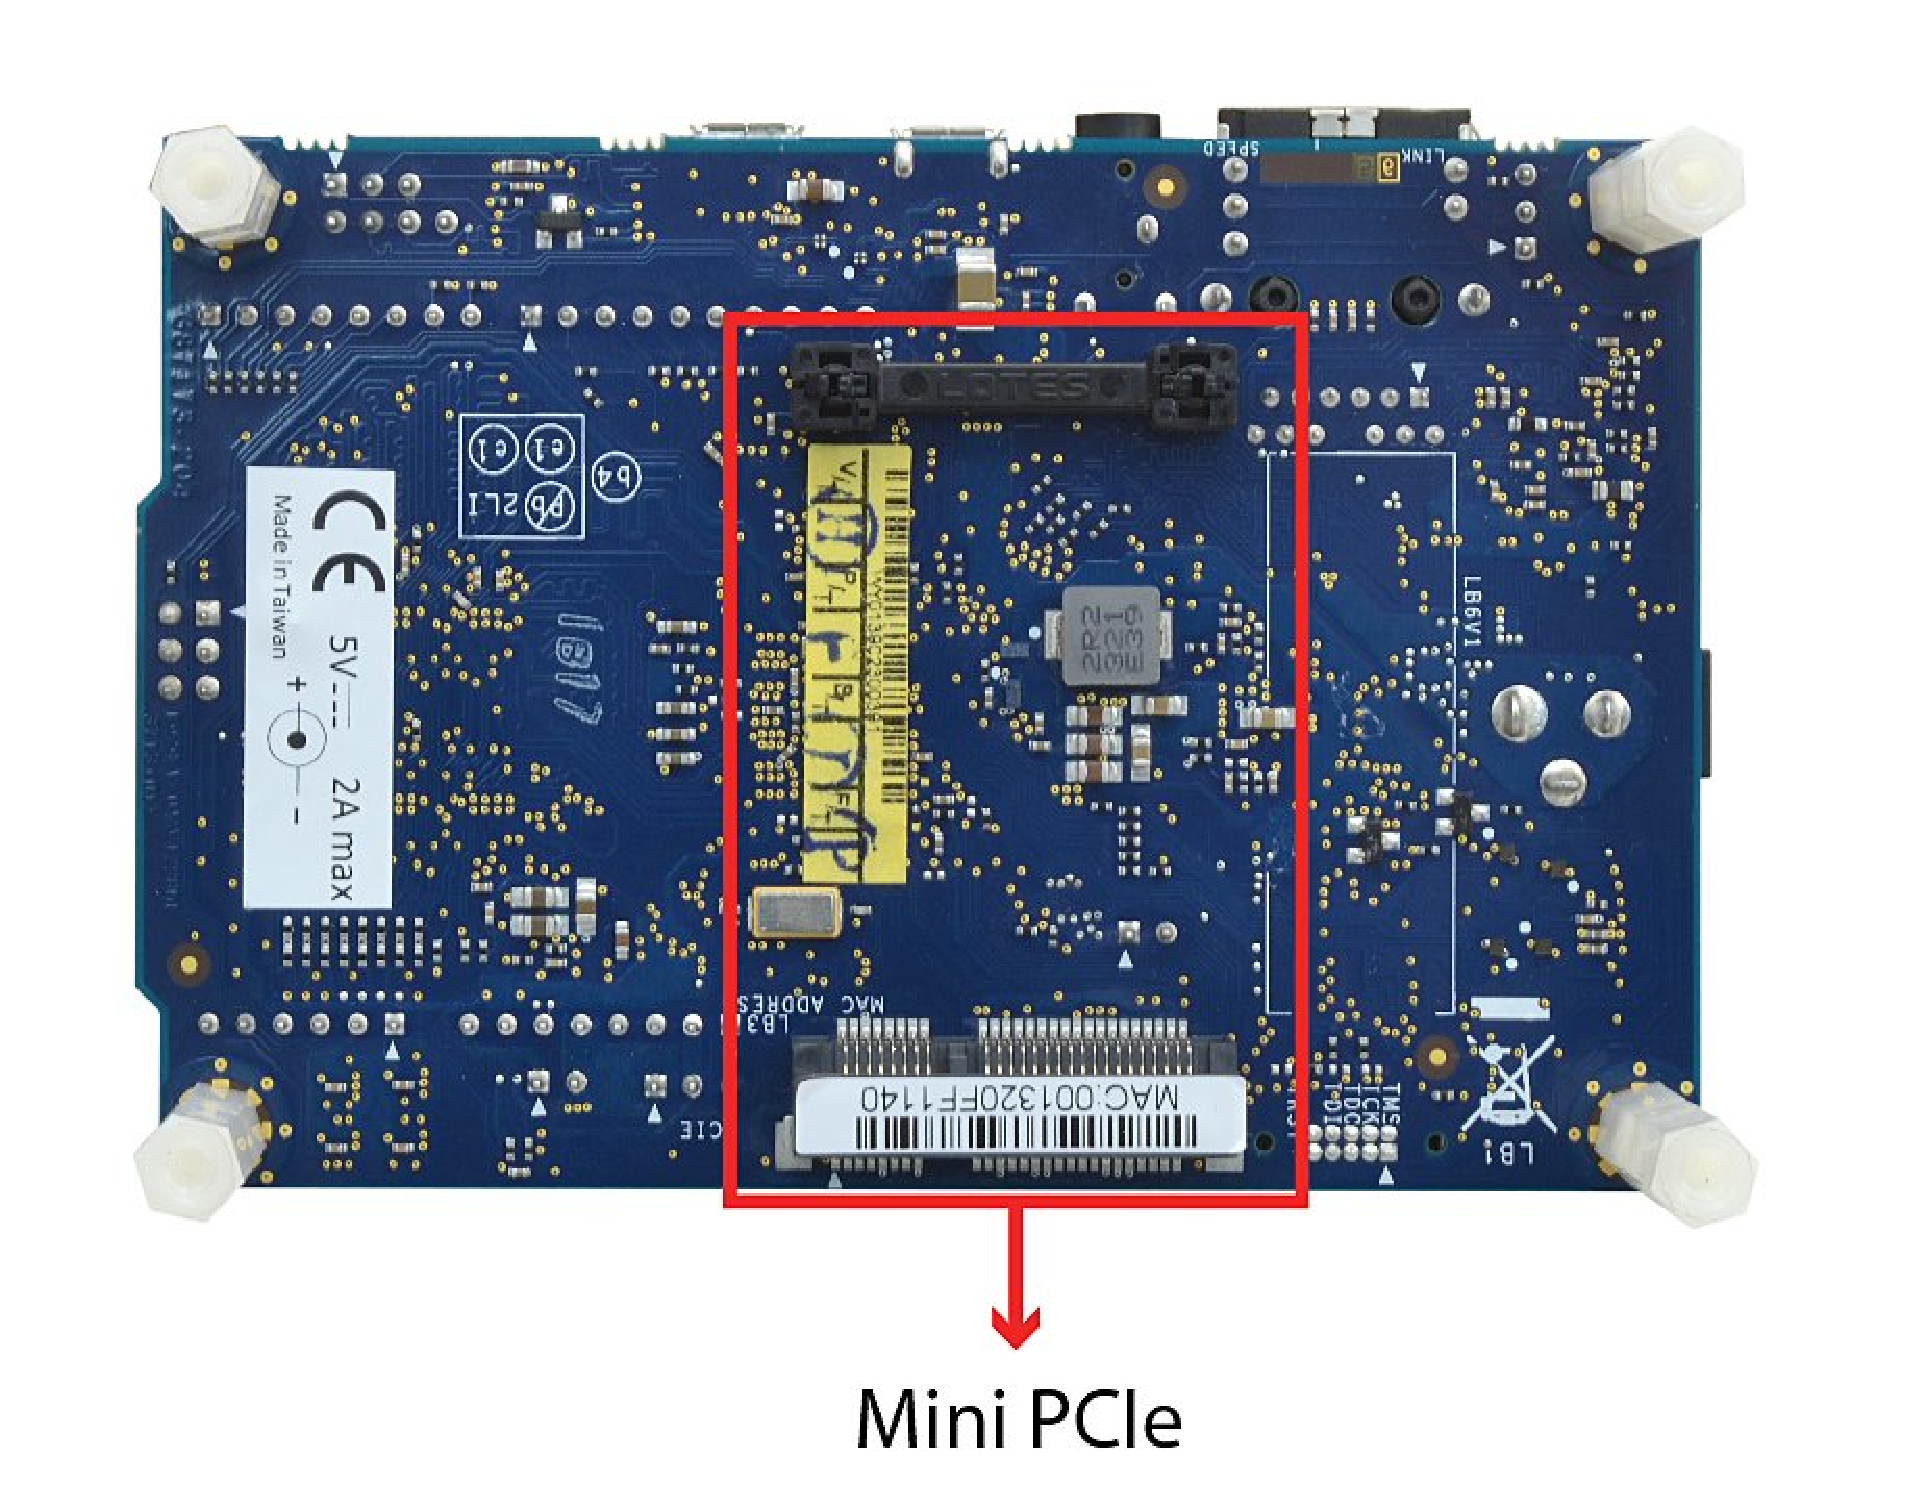
\includegraphics[width=0.5\textwidth]{figs/PCI1.eps}
	\caption{Estrutura da c�lula de mem�ria DRAM}
	\label{DRAM1}
\end{figure}


\begin{itemize}
	\item Conex�es para o barramento PCI Express x1
	\item Conex�es para USB 2.0 
	\item Conex�es para SMBus
	\item Conex�es para LEDs de diagnostico de conex�es wireless
	\item Conex�es para SIM Card 
	\item Conex�es para outras extens�es PCI
	\item Sa�da de 1.5V e 3.3 V 
\end{itemize}




\subsubsection{USB}

USB ou \textit{Universal Serial Bus} � um padr�o cabos, conectores e protocolos. O prop�sito do USB � padronizar a comunica��o com equipamentos perif�ricos como teclados, cameras, impressoras, telefones, etc. USB j� passou por tr�s padroniza��es: 
\begin{itemize}
	\item USB 1.0 com velocidade m�xima de transmiss�o de dados de 12 Mbits/s
	\item USB 2.0 com velocidade m�xima de transmiss�o de dados 480 Mbits/s
	\item USB 3.1 com velocidade m�xima de transmiss�o de 10 dados Gbits/s
\end{itemize}

Para comunica��o com perif�ricos, USB j� tem conseguido subsituir com sucesso a comunica��o serial e paralela.

A topologia USB � assim�trica em formatado de estrela com um dispositivo central (Host), como mostrado no exemplo da Figura \ref{USB3}. 	

Quando um novo equipamento � conectado, o sistema operacional do dispositivo central, a placa galileo por exemplo, detecta a nova conex�o e solicita o driver do equipamento para possibilitar a comunica��o. Como mostrado na Figura \ref{USB1}, os cabos e conex�es USB obedecem os padr�es de duas classes: a classe A e a classe B.

\begin{figure}[t]
	\centering
	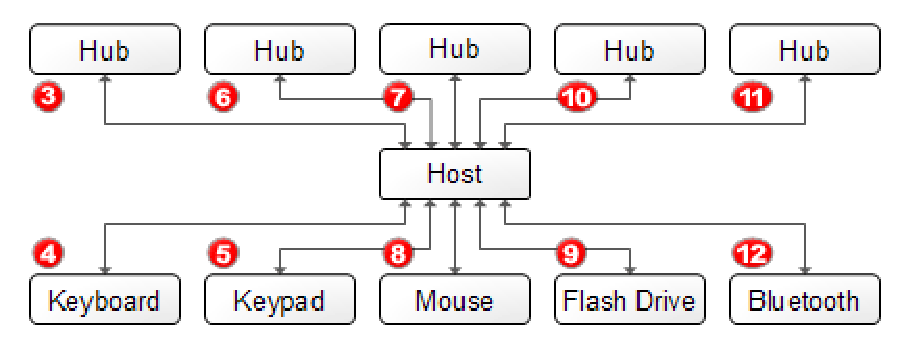
\includegraphics[width=0.6\textwidth]{figs/USB3.eps}
	\caption{Exemplo: Topologia Estrela USB}
	\label{USB3}
	\source{http://www.usblyzer.com/usb-topology.htm}
\end{figure}

Quando o dispositivo central � ligado, � definido para cada dispositivo conectado um endere�o. Tal processo inicial � chamado de \textit{enumera��o}. Durante a \textit{enumera��o}, � tamb�m solicitado a cada equipamento o tipo de transfer�ncia de dados a ser realizado com ele:


\begin{itemize}
	\item Transfer�ncia de dados por meio de interrup��o: Transfer�ncia de dados pouco frequente e de baixa quantidade, como transfer�ncia com teclado e mouse. Nesse caso, vale a pena interromper o sistema operacional.
	
	\item Transfer�ncia de dados por meio de pacotes: Transfer�ncia de dados pouco frequentes e de grande quantidade de dados, como, por exemplo, a transfer�ncia realizada para impressoras. Nesse caso, um bloco de dados e transferido de uma vez s� pela porta USB.
	\item Transfer�ncia de dados is�crono(tempo real): Transfer�ncia de dados frequente e cont�nua, como as necess�rias num alto falante.
\end{itemize}

Para cada uma das formas de transfer�ncia de dados supracitadas, � reservado pelo USB a largura de banda necess�ria em frames de largura de banda.

\begin{figure}[t]
	\centering
	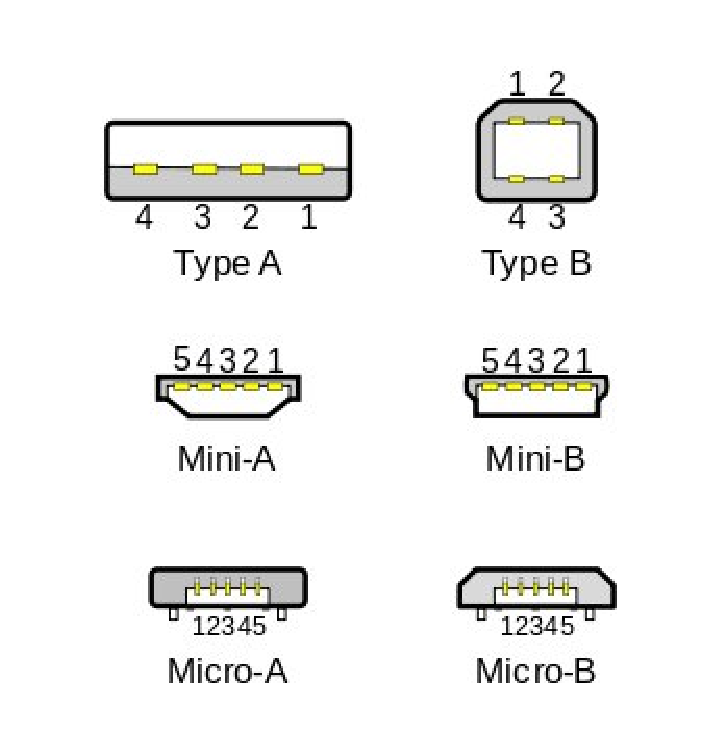
\includegraphics[width=0.45\textwidth]{figs/USB1.eps}
	\caption{Pinos USB }
	\label{USB1}
	\source{http://www.robotizando.com.br/pinagem\_usb.php}
\end{figure}




\subsubsection{JTAG}

JTAG(Joint Test Action Group) � a padroniza��o IEEE-1149.1 usada para testes de circuitos impressos. JTAG foi criada para ajudar no problema da crescente dificuldade de testar circuitos associada com a crescente diminui��o dos tamanhos do circuitos. Como mostrado na Figura \ref{JTAG1}, a implementa��o mais simples de JTAG requer 4 fios para sinaliza��o:

\begin{figure}[H]
	\centering
	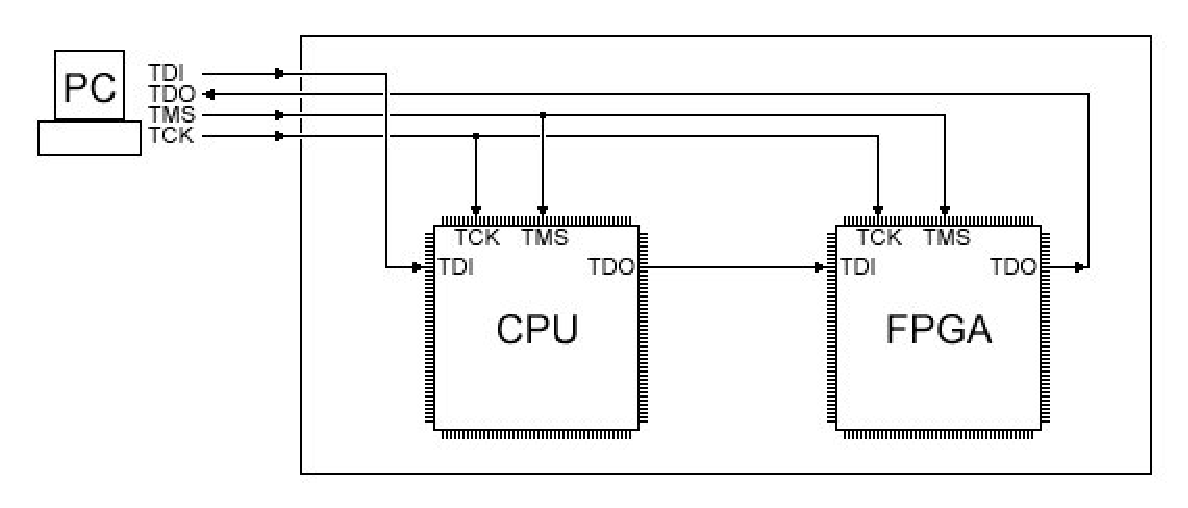
\includegraphics[width=0.8\textwidth]{figs/JTAG1.eps}
	\caption{JTAG monitorando a conex�o de um CPU com uma FPGA }
	\source{https://courses.cit.cornell.edu/ee476/FinalProjects/s2009/jgs33\_rrw32/Final20Paper/}
	\label{JTAG1}
\end{figure}

\begin{itemize}
	\item TDI: Pino para sinal de entrada para a query de teste.
	\item TDO: Pino para sinal de sa�da para a query de teste.
	\item TCK: Sinal do rel�gio de sicroniza��o do JTAG. Todos outros sinais(TDI, TDO, TMS) s�o s�ncronos a esse sinal. 
	\item TMS: Sinal para controlar o estado da m�quina de estados interna ao JTAG, a qual tem 16 estados distintos, como mostrado na figura \ref{JTAG2}.
\end{itemize}



\begin{figure}[H]
	\centering
	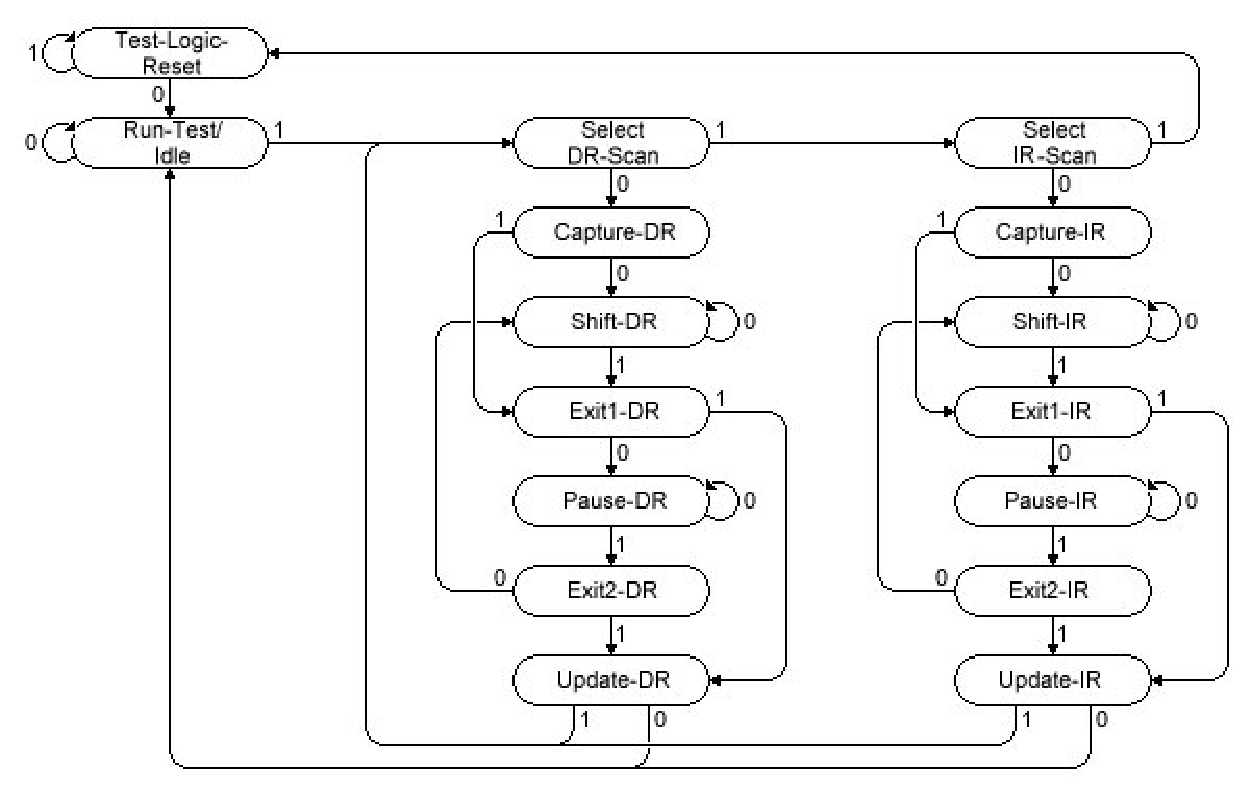
\includegraphics[width=0.7\textwidth]{figs/JTAG2.eps}
	\caption{M�quina de estados - JTAG}
	\label{JTAG2}
	\source{https://courses.cit.cornell.edu/ee476/FinalProjects/s2009/jgs33\_rrw32/Final20Paper/}
	
\end{figure}

Na m�quina de estados mostrada em \ref{JTAG2}, geralmente a JTAG � levada para os estados \textit{Shift-DR}, em primeira inst�ncia, e, ap�s isso, levada para o estado \textit{Shift-IR}, onde o dado � coletado. \textit{Shift-DR} e \textit{Shift-IR} tem o mesmo tamanho \textit{N} de bits. Por exemplo, se \textit{Shift-DR} e \textit{Shift-IR} tiverem 6 bits de tamanho, ap�s 6 clock realizados no TCK, o dado que chegou no \textit{Shift-IR} chega no \textit{Shift-DR}.

A figura \ref{JTAG3} mostra fluxo de dados de ida e volta num debug JTAG: JTAG -> CPU -> FPGA. O dado sa� pelo pino TDI, percorre a CPU e a FPGA e volta no pino TDO sendo tudo isso controlado pelo pino TMS tendo todos esses pinos sincronizados pelo pino TCK.

\begin{figure}[H]
	\centering
	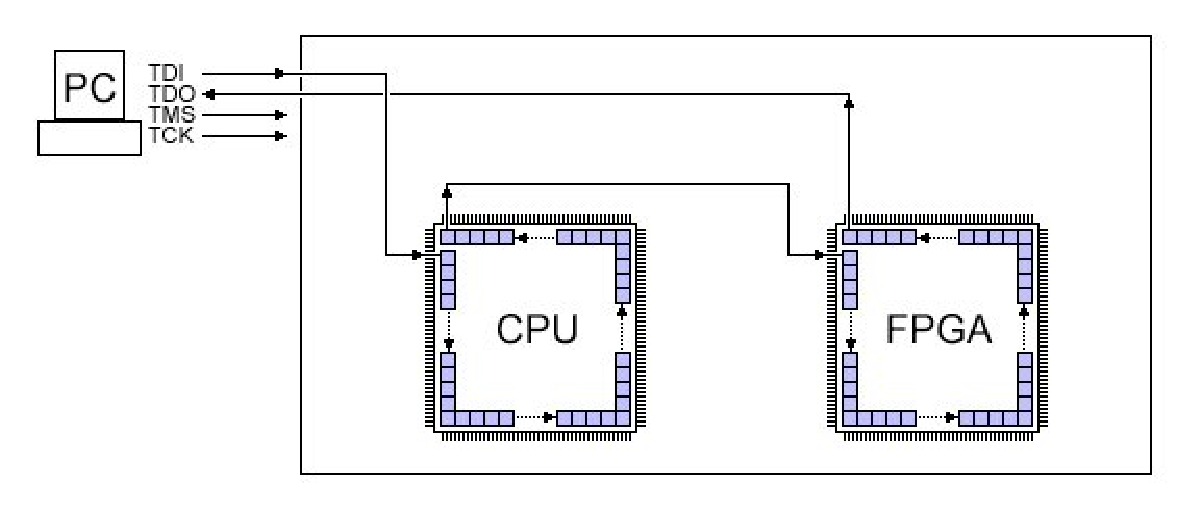
\includegraphics[width=0.8\textwidth]{figs/JTAG3.eps}
	\caption{Fluxo de dados num debug JTAG}
	\label{JTAG3}
	\source{http://www.fpga4fun.com/JTAG.html}
\end{figure}

A verifica��o de entrada e sa�da, inclu�ndo o tempo de tais eventos, com testes JTAG tornou poss�vel testes complexos em circuitos integrados.

A placa Galileo, como grande partes dos circuitos integrados atuais, possui 9 pinos pr�prio para debug com JTAG.

















\section{Proposta de curso}
\label{curso}
A disciplina proposta seguir� a ementa proposta na tabela \ref{ementa}. Na ementa antiga, na qual est� se baseia, a propor��o entre horas de aulas te�ricas e pr�ticas � de 4 para 2 horas. Foi proposta a troca para 4 horas de atividades pr�ticas e 2 horas de atividades te�ricas. 

As atividades pr�ticas n�o devem ser apenas laborat�rias, mas devem contemplar, tamb�m, os seguintes aspectos relativos a ger�ncia de projetos seguindo a metodologia Scrum:

\begin{enumerate}
	\item Reuni�es das equipes Scrum formadas pelos alunos para:
		\subitem  Atualiza��o do quadro de atividades Scrum (\textit{Scrum Backlog}).
		\subitem  Reuni�es de revis�o de \textit{Sprint}
		\subitem  Aprendizagem colaborativa.
		\subitem  Desenvolvimento de projetos propostos.
		\subitem  Reuni�es com o professor que atuar� como \textit{Scrum Master}. 
\end{enumerate}

\begin{table}[H]
	\centering
	\caption{Proposta de ementa}
	\label{ementa}
	\begin{tabular}{|c|c|}
		\hline
		\multicolumn{2}{|c|}{\textbf{CIC - Computa��o b�sica e t�picos em aprendizagem ativa e eletr�nica}}                                                                                                                                                                                                                                                                                                                                                                                                                                                                                                                                                                                                                                                                                                                                                                                                        \\ \hline
		\textbf{Cr�ditos}       & 6 (Teoria:2, Pr�tica:4), $1^{0}$ per�odo                                                                                                                                                                                                                                                                                                                                                                                                                                                                                                                                                                                                                                                                                                                                                                                                                                         \\ \hline
		\textbf{Ementa}         & \begin{tabular}[c]{@{}c@{}}Estudo dos seguintes t�picos de computa��o:\\ 1)Hist�rico da computa��o. Sistemas de numera��o.\\  2)Arquitetura de Computadores.Linguagens formais.\\  3)Algoritmos e programas. Programa��o estruturada.\\ 4) Identificadorese tipos.\\  5)Operadores e express�es. \\ 6)Estruturas de controle: condicional e repeti��o.\\ 7)Entrada e sa�da de dados. \\ 8)Estruturas de dados est�ticas:\\  9)agregados homog�neose heterog�neos.\\ 10) Itera��o e recurs�o.\\ 11) Subalgoritmos.\\  12)Implementa��o de solu��es\\ utilizando o fragmento estruturado\\  de uma linguagem de programa��o\\ \\ Aplicando os seguintes conceitos de eletr�nica b�sica:\\ 1)Circuitos\\ 2)Resistores e Capacitores\\ 3)Lei de Ohm\\ 4) Leis de Kirschoof\\ 5)Sensores\\ 6) Interruptores\\ 7) Programa��o de microcontroladores baseados\\ em Arduino\end{tabular} \\ \hline
		\textbf{Bibliografia}   & \begin{tabular}[c]{@{}c@{}}Basic Electronics. New York: Dover Publications, 1973. ISBN 978-0486210766.{[}33{]} \\ KERNIGHAN, B. The C programming language. Englewood Cliffs, N.J: Prentice Hall, \\ 1988.ISBN 978-0131103627.\end{tabular}                                                                                                                                                                                                                                                                                                                                                                                                                                                                                                                                                                                                                                      \\ \hline
		\textbf{Pr�-requisitos} & Sem pr�-requisitos                                                                                                                                                                                                                                                                                                                                                                                                                                                                                                                                                                                                                                                                                                                                                                                                                                                               \\ \hline
	\end{tabular}
\end{table}

Para se construir um projeto Scrum, como exposto na se��o \ref{EstudoScrum}, para o contexto educacional da teoria de masteriza��o de habilidades proposta por Bloom, os seguintes passos  s�o necess�rios:

\begin{enumerate}
	\item Realizar adapta��o dos princ�pios e fluxo da metodologia Scrum, em conjunto com os princ�pios da metodlogia de \textit{masteriza��o de habilidades} para o contexto educacional desejado.
	\item Definir os objetivos educacionais na forma \textit{de caracter�sticas de produto} utilizando a taxonomia de Bloom para criar as \textit{User Stories} e \textit{Epics} e definir os crit�rios de aprova��o para cada objetivo de masteriza��o.
	\item Criar atividades com a placa Galileo de acordo com o cont�udo program�tico estabelecido
	
		 
\end{enumerate}
Cada uma das atividades listadas acima ser� tratada, neste trabalho, em uma se��o em separado.


\subsection{Aprendizagem por masteriza��o e Scrum adaptados ao curso de Algoritmos e Programa��o de Computadores}

Nesta se��o � apresentada uma proposta de adapta��o da metodologia Scrum para aplica��o na disciplina \textit{Algoritmos e Programa��o de Computadores}. 

A tabela \ref{tabEduScrum} mostra um resumo de todo fluxo mostrado na figura \ref{scrum2} 
e, ao lado, a proposta de adapta��o:
% Please add the following required packages to your document preamble:
% \usepackage{booktabs}
\begin{table}[H]
	\centering
	\caption{Scrum aplicado � \textit{Algoritmos e Programa��o de Computadores}}
	\label{tabEduScrum}
	\begin{tabular}{@{}cll@{}}
		\toprule
		\textbf{}                                                                                                            & \multicolumn{1}{c}{\textbf{Scrum}}                                                                                                                                                                                                                                                                                                                                                                                                                                                                                                                                                                                                                                                                          & \multicolumn{1}{c}{\textbf{Scrum + Masteriza��o de habilidades}}                                                                                                                                                                                                                                                                                                                                                                                                                                                                                                                                                                                                                                    \\ \midrule
		\multicolumn{1}{|c|}{\textbf{\begin{tabular}[c]{@{}c@{}}Por que \\ utilizar Scrum?\end{tabular}}}                    & \multicolumn{1}{l|}{\begin{tabular}[c]{@{}l@{}}-Uso de ciclo curtos de \\ desenvolvimento e \\ revis�o(Sprints)\\ -Revis�o frequente dos\\  requisitos de projeto a \\ cada Sprint\\ - Melhora cont�nua\\ -Valor agredado acima \\ de obedici�ncia a cronograna\\  e processos\\ - Entrega cont�nuade Valor\end{tabular}}                                                                                                                                                                                                                                                                                                                                                                                   & \multicolumn{1}{l|}{\begin{tabular}[c]{@{}l@{}}1)Verifica��o,de n�veis \\ de aprendizagem frequentes\\ 2)Aumento, a cada \\ Sprint, da responsabiliza��o\\  pessoal dos alunos com \\ rela��o a seus estudos\end{tabular}}                                                                                                                                                                                                                                                                                                                                                                                                                                                                          
		\\ \midrule
	\end{tabular}
\end{table}

\begin{table}[H]
	\centering
	\caption*{}
	%\label{}
	\begin{tabular}{@{}cll@{}}
		%\toprule
		\textbf{}                                                                                                            & \multicolumn{1}{c}{\textbf{Scrum}}                                                                                                                                                                                                                                                                                                                                                                                                                                                                                                                                                                                                                                                                          & \multicolumn{1}{c}{\textbf{Scrum + Masteriza��o de habilidades}}                                                                                                                                                                                                                                                                                                                                                                                                                                                                                                                                                                                                                                    
		
		%\\ \midrule
		
		\\ \midrule
		\multicolumn{1}{|c|}{\textbf{Pap�is}}                                                                                & \multicolumn{1}{l|}{\begin{tabular}[c]{@{}l@{}}- Product Owner\\  Representante da voz do cliente\\ -Scrum Master\\ Gerente do time Scrum\\  respons�vel por certificar-se\\  que os princ�pios Scrum est�o\\  sendo seguidos pela equipe\\  e tamb�m respons�vel por\\  coletar os requisitos \\ de projeto junto ao\\  Product Owner\\ -Time Scrum -\textgreater Equipe \\ respons�vel por desenvolver\\  os requisitos de projeto\\  descritos, inclusive, \\ por meio de User Stories\end{tabular}}                                                                                                                                                                                                     & \multicolumn{1}{l|}{\begin{tabular}[c]{@{}l@{}}Product Owner - Professor\\ \\ \\ Scrum Master - Professor\\ (enquanto os alunos n�o\\  estiverem familiarizados\\  com a metodologia Scrum\\ e prontos para auto-ger�ncia\\  de seus,estudos)\\ \\ \\ Time Equipe Scrum - Equipe\\  de at� 4 estudantes\\  respons�veis( sem contar\\  o professor) por concluir,\\ conjuntamente,  os objetivos\\  de aprendizagem\\ descritos por meio da \\ taxonomia de Bloom.\\ \\ \\ A equipe Scrum deve eleger\\  um representante novo a \\ cada Sprint para se comunicar\\ diretamente com o professor \\ (Scrum Master) e planejar \\ as atividades e meios \\ de verifica��o conjuntamente\end{tabular}} 
		
		\\ \midrule
		                                                                               \\ \bottomrule
	\end{tabular}
\end{table}

\begin{table}[H]
	\centering
	\caption*{}
	%\label{}
	\begin{tabular}{@{}cll@{}}
		%\toprule
		\textbf{}                                                                                                            & \multicolumn{1}{c}{\textbf{Scrum}}                                                                                                                                                                                                                                                                                                                                                                                                                                                                                                                                                                                                                                                                          & \multicolumn{1}{c}{\textbf{Scrum + Masteriza��o de habilidades}}                                                                                                                                                                                                                                                                                                                                                                                                                                                                                                                                                                                                                                    
		
		\\ \midrule
		
		
		\multicolumn{1}{|c|}{\textbf{\begin{tabular}[c]{@{}c@{}}Fase 1 -\\  In�cio \\ Defini��o\\  de projeto\end{tabular}}} & \multicolumn{1}{l|}{\begin{tabular}[c]{@{}l@{}}1) Criar vis�o de projeto \\   2) Identificar Scrum \\ Master e Skateholders\\ 3) Formar Time Scrum                     \\   4) Desenvolver Epics\\     (Conjunto de user stories)\\ 5) Criar conjunto priorit�rio\\  de caracter�sticas do produto               \\ 6) Criar um plano de\\ desenvolvimento do produto \\ em Sprints sequenciais\end{tabular}}                                                                                                                                                                                                                                                                                               & \multicolumn{1}{l|}{\begin{tabular}[c]{@{}l@{}}1),Criar objetivos educacionais\\  com a taxonomia de Bloom\\ 2)Scrum Master = Professor\\ Stakeholders =,alunos, \\ familias, governo,etc\\ 3) Formar grupos de 3 ou \\ 4 alunos , preferencialmente\\  n�o amigos e com \\ caracter�sticas complementares\\ 4) Dividir os objetivos\\ educacionais em m�dulos\\ 5) Criar plano de ascen��o\\  dos alunos nos n�veis \\ cognitivos de bloom para os \\ conte�dos especificados\\ 6) Criar especifica��o de \\ Sprint com  os objetivos\\  educacionais\end{tabular}}                                                                                 

		  \\ \midrule
		  
		  \multicolumn{1}{|c|}{\textbf{\begin{tabular}[c]{@{}c@{}}Fase 2 - Plano \\ de Projeto  e \\ Estima��o\end{tabular}}}  & \multicolumn{1}{l|}{\begin{tabular}[c]{@{}l@{}}1)Crit�rios de aceita��o\\  s�o criados (a ser feito\\  pelo Product Owner \\ juntamente com o Scrum\\  Team)          \\ 2) Scrum Master e time \\ estimam o esfor�o\\ necess�rio para desenvolver\\ as User Stories                                        \\   3)Scrum master e time\\  se comprometem\\  a desenvolver o produto\\  de acordo com as Epics\\ (Conjunto de User Stories) \\ e crit�rios de aceita��o                             \\ 4)User Stories\\  s�o divididas em subtarefas \\ para criar uma Task List     \\ 5) Time Scrum se reune\\  para decidir quais tarefas\\  ser�o realizadas na \\ Sprint (Sprint Backlog)\end{tabular}} & \multicolumn{1}{l|}{\begin{tabular}[c]{@{}l@{}}1) O professor,  a cada Sprint,\\  deve deixar claro quais ser�o\\ os crit�rios de masteriza��o\\  de habilidades preferencialmente\\ utilizandoa taxonomia \\ de Bloom\\ 2)Professor � respons�vel, \\ a cada Sprint, por estimar o \\ esfor�o necess�rio por parte da\\ turma para as masteriza��es \\ desejadas.\\  \\ A participa��o dos representantes\\  de equipes com rela��o � defini��o\\  de planos Sprint � crescente ao\\  longo dos Sprints.\end{tabular}}                                                                                                                                                                             
		 \\ \bottomrule
		  
		                                               
		
\end{tabular}
\end{table}

\begin{table}[H]
	\centering
	\caption*{}
	%\label{}
	\begin{tabular}{@{}cll@{}}
		%\toprule
		\textbf{}                                                                                                            & \multicolumn{1}{c}{\textbf{Scrum}}                                                                                                                                                                                                                                                                                                                                                                                                                                                                                                                                                                                                                                                                          & \multicolumn{1}{c}{\textbf{Scrum + Masteriza��o de habilidades}}                                                                                                                                                                                                                                                                                                                                                                                                                                                                                                                                                                                                                                    
		
		\\ \midrule
		
		
		\multicolumn{1}{|c|}{\textbf{\begin{tabular}[c]{@{}c@{}}Fase 3 - \\ Implementa��o\end{tabular}}}                     & \multicolumn{1}{l|}{\begin{tabular}[c]{@{}l@{}}1)Criar os "entreg�veis"\\  do Sprint \\   2) Realizar reuni�es\\  di�rias r�pidas de no\\  m�ximo 15 minutos para\\   discutir problemas\\  e progresso       \\   3) Atualizar o quadro\\  Scrum  antes de iniciar\\  o dia de trabalho\end{tabular}}                                                                                                                                                                                                                                                                                                                                                                                                      & \multicolumn{1}{l|}{\begin{tabular}[c]{@{}l@{}}1)Estudar o conte�do especificado\\  emgrupo com a ajuda do Scrum \\ Master(Professor)\\ 2) Realizar reuni�es di�rias r�pidas\\  de no m�ximo 15 minutos\\  para discutir problemas e progresso\\ 3)A equipe Scrum decide os meios\\  de aprendizagem que usar�o com\\  aux�lio do professor. A cada Sprint,\\  a equipe Scrum deve ficar mais\\  livre para decidir os meios mais\\  eficientes de,aprendizagem\\ 4) Atualizar o quadro Scrum de \\ ( A FAZER , FAZENDO, FEITO)\end{tabular}}                                                                                       
		
		\\ \midrule
		\multicolumn{1}{|c|}{\textbf{\begin{tabular}[c]{@{}c@{}}Fase 4 - \\ Fim de Sprint;\\ Revis�o\\  e Retrospecto\end{tabular}}}               & \multicolumn{1}{|c|}{\begin{tabular}[c]{@{}l@{}}1)Os,entreg�veis s�o \\ mostrados aos \\ Stakeholders\\ 2) Essas reuni�es s�o\\  feitas para garantir\\  a aprova��o do produto\\  desenvolvido e fazer\\  os ajustes necess�rios\\  o mais r�pido poss�vel\\ 3) O Scrum Master e o\\  time Scrum se reunem\\  para discutir o que foi\\  aprendido no Sprint\\ 4) Informa��o � documentada\\  para futuros Sprints\end{tabular}}                                                                                                                                                                                                                                                                                                 & \multicolumn{1}{|c|}{\begin{tabular}[c]{@{}l@{}}1)A equipe Scrum desenvolve\\  testes r�pidos( para serem\\  resolvidos em no m�ximo \\ 20 minutos) para que as outras\\  equipes resolvam do conte�do\\  estudado no Sprint. O gabarito\\  deve ser entregue ao professor\\  antes da aplica��o dos testes \\ para que este verifique-os e \\ decida quais testes\\ ser�o aplicados\\ 2) A equipe resolve, no tempo\\ estipulado, os testes compartilhados\\ 3) Ap�s os testes de unidade,\\  o professor e os alunos tem\\  uma aula para revisar o que\\ foi aprendido de acordo com\\  os objetivos educacionais tra�ados\end{tabular}}                                                                               \\ \bottomrule
		
		
	\end{tabular}
\end{table}

\subsubsection{Defini��o de objetivos educacionais na forma da metologogia Scrum}

Para realizar a defini��o dos objetivos educacionais, foi utlizada a plataforma web scrumdo \textsuperscript{\textregistered} sendo cadastrados os seguintes objetivos educacionais pr�prios da disciplina \textit{Algoritmos e Programa��o de Computadores}:

\begin{enumerate}
	\item O hist�rico da computa��o
	\item Organiza��o b�sica de um computador
	\item Introdu��o ao conceito de algoritmo
	\item Pseudoc�digo e Fluxograma
	\item Tipos de vari�veis de mem�ria
	\item Operadores e express�es
	\item Algoritmos sequenciais
	\item Algoritmos com alternativas (simples, compostas, aninhadas e de m�ltipla escolha)
	\item Algoritmos com repeti��o (com teste no in�cio, com teste no fim e com vari�vel de controle)
	\item Algoritmos com vetores e matrizes
	\item Subalgoritmos, passagem de par�metros,
	\item Ponteiros
	\item Recursividade
	\item Registros
	\item Arquivos
	\item Ordena��o e busca
	
\end{enumerate}

Aos objetivos listados, devem ser inclu�dos os seguintes objetivos educacionais relativos a placa Intel\textsuperscript{\textregistered} Galileo e eletr�nica b�sica:

\begin{enumerate}
	\item Leis b�sicas de eletr�nica( Leis de Kirschoff)
	\item Sistema da placa Galileo
	\item Ferramentas b�sicas de prototipa��o eletr�nica
	\item Fundamentos de programa��o em Galileo
	\item Introdu��o a sensores
	\item Intera��o com sensores
	\item Uso de displays
	\item Motores
	\item T�pico mais avan�ado em eletr�nica a ser escolhido com a Turma (Comunica��o Ethernet ou Internet, Comunica��o sem fio, Uso de placa SD de armazenamento de dados, uso de interrup��es, Circuitos integrados perif�ricos, controle de altas cargas, etc)
\end{enumerate}

A Figura \ref{scrumdo1} mostra o plataforma web scrumdo \textsuperscript{\textregistered} para cadastramento de quadros scrum pertinentes.
\begin{figure}[H]
	\centering
	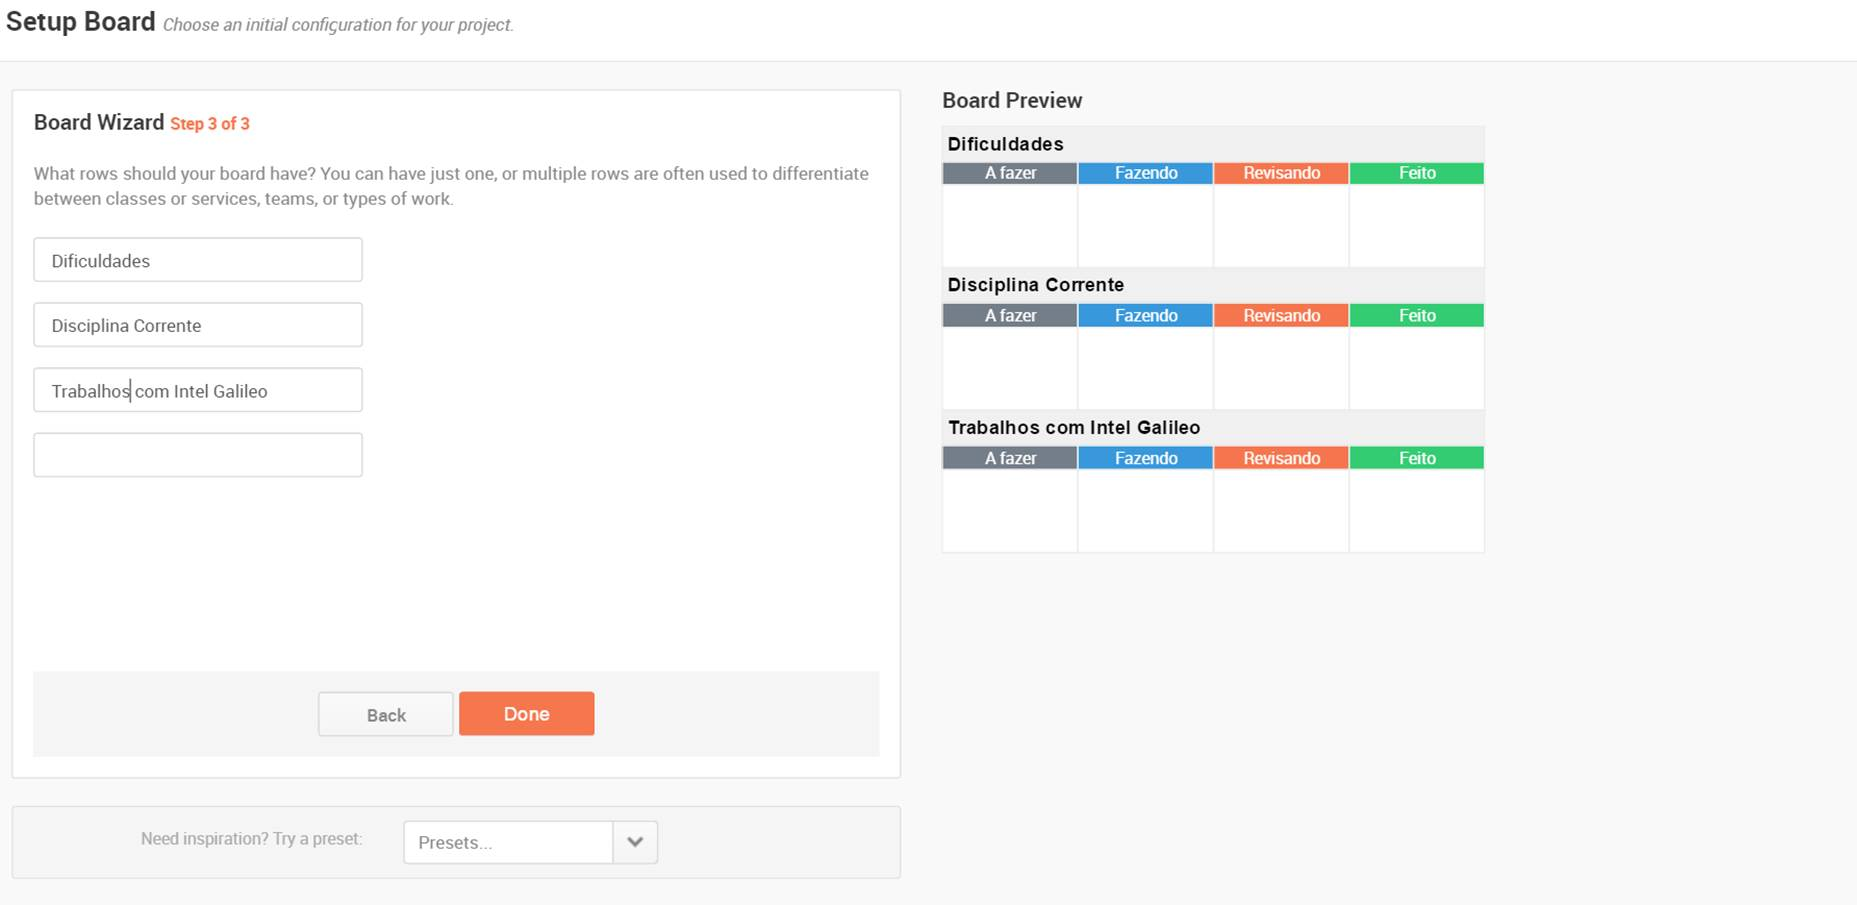
\includegraphics[width=1\textwidth]{figs/scrumdo1.eps}
	\caption{Plataforma scrumdo: Formato dos quadros Scrum planejados para a disciplina \textit{Algoritmos e Programa��o de Computadores}}
	\label{scrumdo1}
\end{figure}

A Figura \ref{scrumdo2} mostra os quadros \textit{Dificuldades} \textit{Algoritmos e Programa��o de Computadores}, \textit{Aplica��o com Galileo}. A disposi��o dos 3 quadros deve refletir a prioridade da turma. As reuni�es de Sprint devem servir para resolver quest�es pendentes posta no quadro \textit{Dificuldades}.


\begin{figure}[H]
	\centering
	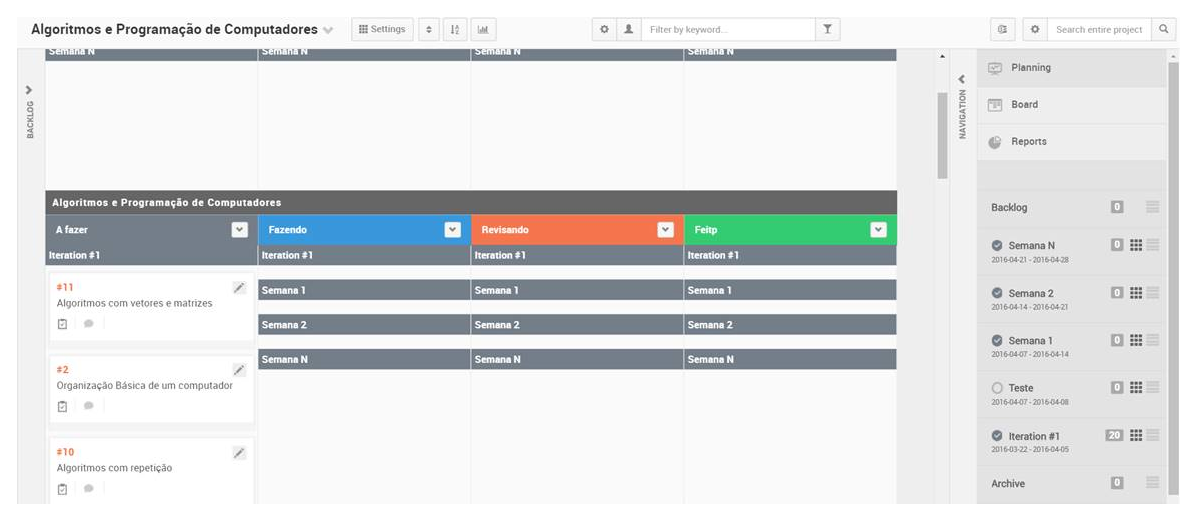
\includegraphics[width=1\textwidth]{figs/scrumdo2.eps}
	\caption{Plataforma scrumdo: Quadros Scrum criados e objetivos educacionais, segundo a Taxonomia de Bloom escritos \textit{Algoritmos e Programa��o de Computadores}}
	\label{scrumdo2}
\end{figure}

Pode-se, por meio da plataforma, selecionar sub-objetivos. No caso deste trabalho, para cada t�pico listado para as pr�ticas com a placa Galileo, foram criados objetivos educacionais para os tr�s primeiros n�veis cognitivos identificados por Bloom( N�vel de Conhecimento, Compreens�o a Aplica��o).


\begin{figure}[H]
	\centering
	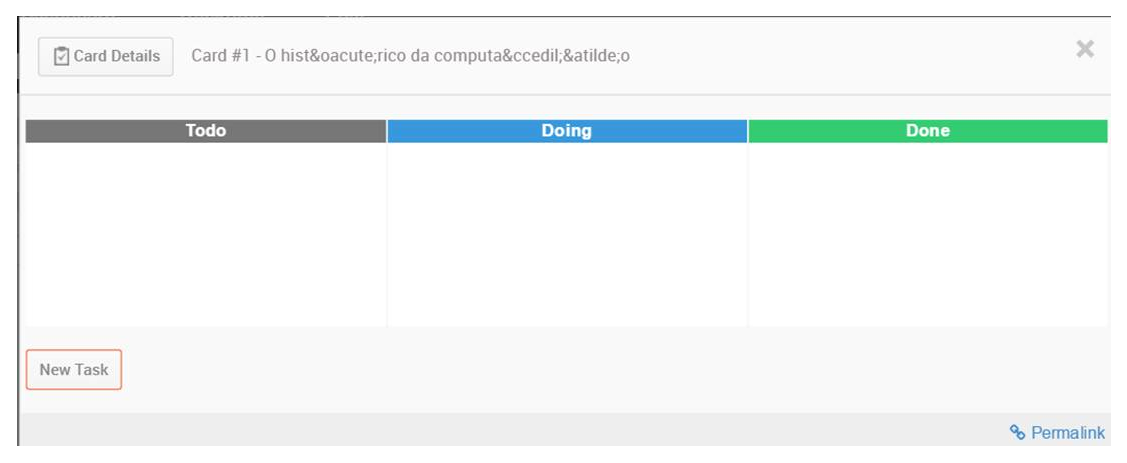
\includegraphics[width=1\textwidth]{figs/scrumdo3.eps}
	\caption{Plataforma scrumdo: Definica��o de sub-objetivos de um objetivo listado no \textit{Product Backlog} \textit{Algoritmos e Programa��o de Computadores}}
	\label{scrumdo3}
\end{figure}

\begin{figure}[H]
	\centering
	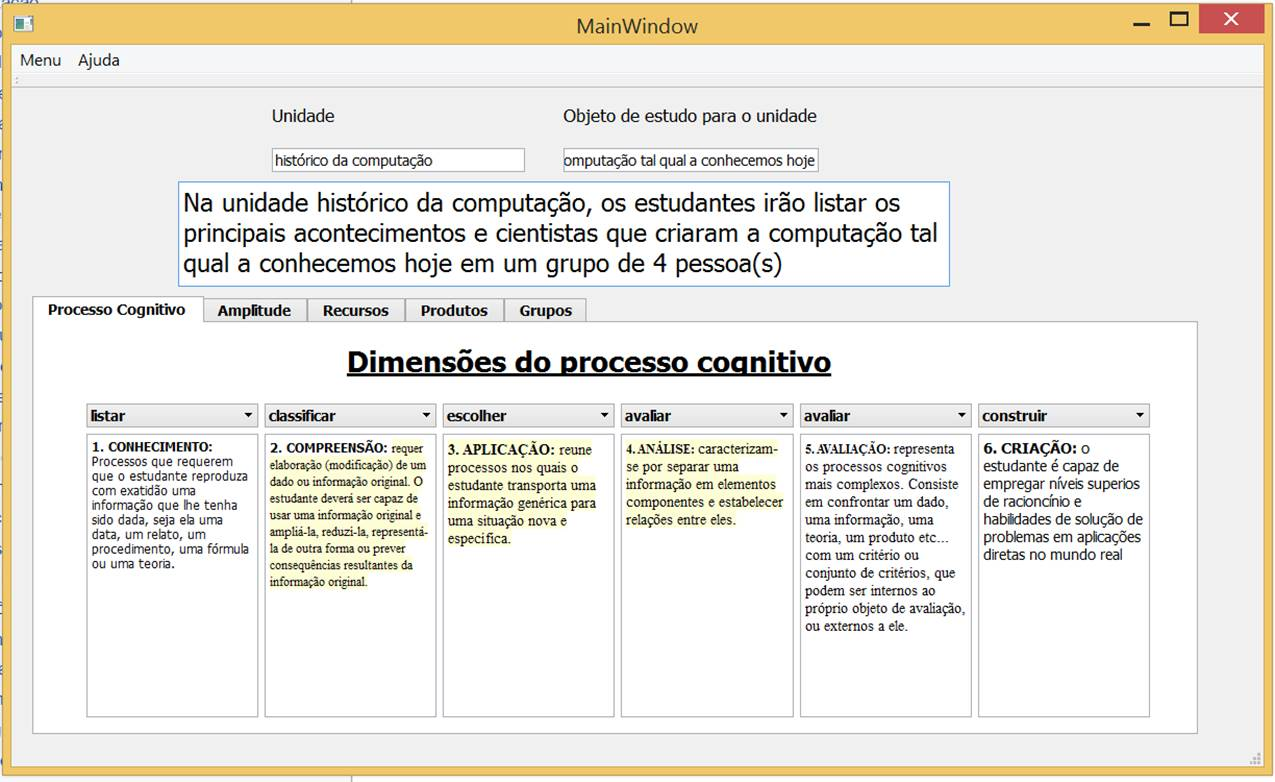
\includegraphics[width=1\textwidth]{figs/app1.eps}
	\caption{Uso do aplicativo desenvolvido em QT para definir os objetivo educacional para o n�vel \textit{Conhecimento}}
	\label{app1}
\end{figure}

\subsubsection{Defini��o de objetivos educacionais para a Disciplina \textit{Algoritmos e Programa��o de Computadores}}

Para especificar cada objetivo educacional, foi utilizado o aplicativo desenvolvido em QT, como descrito anteriomente e como mostrado na Figura \ref{app1}.

A seguinte enumera��o mostra uma poss�vel especifica��o de cada um dos m�dulos de aprendizagem definidos anteriormente seguindo a \textit{Taxonomia de Bloom}:
\begin{enumerate}
	\item O hist�rico da computa��o
		\subitem \textbf{N�vel 1 Conhecimento:}
		Na unidade \textbf{hist�rico da computa��o}, os estudantes ir�o listar os principais acontecimentos e cientistas que criaram a computa��o tal qual a conhecemos hoje em um grupo de 4 pessoa(s).
		\subitem \textbf{N�vel 2 Compreens�o:}
		Na unidade hist�rico da computa��o, os estudantes ir�o explicar a relev�ncia da computa��o no mundo moderno em um grupo de 4 pessoa(s).
		\subitem \textbf{N�vel 3 Aplica��o:}
		Na unidade hist�rico da computa��o, os estudantes ir�o escolher, dentre certos sistemas computacionais exposto, qual seria aquele(s) que mais se adequariam ao contexto exposto em um grupo de 4 pessoa(s).
	\item Organiza��o b�sica de um computador
		\subitem \textbf{N�vel 1 Conhecimento:}
		Na unidade organiza��o b�sica de um computador, os estudantes ir�o enumerar e explicar o funcionamento de todos os sistemas que comp�em um computador em um grupo de 4 pessoa(s).
		\subitem \textbf{N�vel 2 Compreens�o:}
		Na unidade organiza��o b�sica de um computador, os estudantes ir�o classificar computadores quanto a par�metros de desempenho entre outros em um grupo de 4 pessoa(s).
		\subitem \textbf{N�vel 3 Aplica��o:}
		Na unidade organiza��o b�sica de um computador, os estudantes ir�o ilustrar a din�mica de funcionamento de um computador e criar�o um diagrama em um grupo de 4 pessoa(s).
		\item Introdu��o ao conceito de algoritmo
		\subitem \textbf{N�vel 1 Conhecimento:}
	Na unidade introdu��o ao conceito de algoritmo, os estudantes ir�o definir conceitualmente o que s�o algoritmos em um grupo de 4 pessoa(s).
		\subitem \textbf{N�vel 2 Compreens�o:}
		Na unidade introdu��o ao conceito de algoritmo, os estudantes ir�o identificar v�rios tipos diferentes algoritmos em um grupo de 4 pessoa(s).
		\subitem \textbf{N�vel 3 Aplica��o:}
		Na unidade introdu��o ao conceito de algoritmo, os estudantes ir�o empregar um determinado tipo de algoritmo para cada situa��o dada em um grupo de 4 pessoa(s).
	\item Pseudoc�digo e Fluxograma
		\subitem \textbf{N�vel 1 Conhecimento:}
		Na unidade pseudoc�digo e fluxograma, os estudantes ir�o duplicar por meio das ferramentas citadas, situa��es do cotidiano  em um grupo de 4 pessoa(s).
		\subitem \textbf{N�vel 2 Compreens�o:}
		Na unidade pseudoc�digo e fluxograma, os estudantes ir�o selecionar por meio dos pseudoc�digos e fluxogramas j� constru�dos  quais s�o os mais eficientes para cada situa��o dada em um grupo de 4 pessoa(s).
		\subitem \textbf{N�vel 3 Aplica��o:}
		Na unidade pseudoc�digo e fluxograma, os estudantes ir�o programar os primeiros algoritmos em um grupo de 4 pessoa(s).
	\item Tipos de vari�veis de mem�ria
		\subitem \textbf{N�vel 1 Conhecimento:}
		Na unidade tipos de vari�veis de mem�ria, os estudantes ir�o listar todos os tipos de vari�veis em um grupo de 4 pessoa(s).
		\subitem \textbf{N�vel 2 Compreens�o:}
		Na unidade tipos de vari�veis de mem�ria, os estudantes ir�o explicar as diferen�as de usabilidade entre todos os tipo de vari�veis em um grupo de 4 pessoa(s).
		\subitem \textbf{N�vel 3 Aplica��o:}
		Na unidade tipos de vari�veis de mem�ria, os estudantes ir�o escolher dentre todos os tipos de vari�vel de mem�ria, aquelas que melhor se aplicam �s situa��es propostas e explicar o motivo em um grupo de 4 pessoa(s).
	\item Operadores e express�es
		\subitem \textbf{N�vel 1 Conhecimento:}
		Na unidade operadores e express�es, os estudantes ir�o enumerar os v�rios tipos de operadores e express�es na linguagem C e demonstrar seu uso em um grupo de 4 pessoa(s).
		\subitem \textbf{N�vel 2 Compreens�o:}
		Na unidade operadores e express�es, os estudantes ir�o descrever o resultado de v�rias express�es escritas, explicitando os passos desenvolvidos em um grupo de 4 pessoa(s).
		\subitem \textbf{N�vel 3 Aplica��o:}
		Na unidade operadores e express�es, os estudantes ir�o desenvolver programas para solu��o de diversas situa��es propostas em um grupo de 4 pessoa(s).
	\item Algoritmos sequenciais
		\subitem \textbf{N�vel 1 Conhecimento:}
		Na unidade algoritmos sequenciais, os estudantes ir�o definir o conceito, todas express�es e operadores utilizados em um grupo de 4 pessoa(s).
		\subitem \textbf{N�vel 2 Compreens�o:}
		Na unidade algoritmos sequenciais, os estudantes ir�o definir o resultado esperado na utiliza��o de um algoritmo sequencial em um grupo de 4 pessoa(s).
		\subitem \textbf{N�vel 3 Aplica��o:}
		Na unidade algoritmos sequenciais, os estudantes ir�o empregar algoritmos sequencias na solu��o de situa��es diversas em um grupo de 4 pessoa(s).
	\item Algoritmos com alternativas (simples, compostas, aninhadas e de m�ltipla escolha)
		\subitem \textbf{N�vel 1 Conhecimento:}
		Na unidade algoritmos com alternativas, os estudantes ir�o definir os v�rios de operadores condicionais utlizados em C quanto a sua din�mica e utiliza��o em um grupo de 4 pessoa(s).
		\subitem \textbf{N�vel 2 Compreens�o:}
		Na unidade algoritmos com alternativas, os estudantes ir�o identificar o resultado de uma s�rie de condicionais aplicados num algoritmo sequencial em um grupo de 4 pessoa(s).
		\subitem \textbf{N�vel 3 Aplica��o:}
		Na unidade algoritmos com alternativas, os estudantes ir�o construir programas complexos com alternativa condicionais em um grupo de 4 pessoa(s).
		
	\item Algoritmos com repeti��o (com teste no in�cio, com teste no fim e com vari�vel de controle)
		\subitem \textbf{N�vel 1 Conhecimento:}
		Na unidade algoritmos com repeti��o, os estudantes ir�o lembrar a sintaxe correta de todas formas de la�os de repeti��o em C em um grupo de 4 pessoa(s).
		\subitem \textbf{N�vel 2 Compreens�o:}
		Na unidade algoritmos com repeti��o, os estudantes ir�o explicar a diferen�a de usubilidade das formas de la�os de repeti��o em C em um grupo de 4 pessoa(s).
		\subitem \textbf{N�vel 3 Aplica��o:}
		Na unidade algoritmos com repeti��o, os estudantes ir�o construir programas complexos com la�os de repeti��o em um grupo de 4 pessoa(s).
	\item Algoritmos com vetores e matrizes
		\subitem \textbf{N�vel 1 Conhecimento:}
		\subitem \textbf{N�vel 2 Compreens�o:}
		\subitem \textbf{N�vel 3 Aplica��o:}
		Na unidade algoritmos com vetores e matrizes, os estudantes ir�o construir programas complexos com utilizando tais conceitos em um grupo de 4 pessoa(s).
	\item Subalgoritmos e passagem de par�metros
		\subitem \textbf{N�vel 1 Conhecimento:}
		Na unidade subalgoritmos e passagem de par�metros, os estudantes ir�o expor por meio de exemplo e aplica��es, a forma sintaticamente correta de escrita de subalgoritmos e passagem de par�metros em um grupo de 4 pessoa(s)
		\subitem \textbf{N�vel 2 Compreens�o:}
		Na unidade subalgoritmos e passagem de par�metros, os estudantes ir�o identificar todos par�metros e requisitos de para correta escrita de tais rotinas computacionais em um grupo de 4 pessoa(s).
		\subitem \textbf{N�vel 3 Aplica��o:}
		Na unidade subalgoritmos e passagem de par�metros, os estudantes ir�o construir programas complexos, constru�dos sob diversos subalgoritmos, em um grupo de 4 pessoa(s)
	\item Ponteiros
		\subitem \textbf{N�vel 1 Conhecimento:}
		Na unidade ponteiros, os estudantes ir�o listar todas caracter�sticas que definem por completo um ponteiro em um grupo de 4 pessoa(s).
		\subitem \textbf{N�vel 2 Compreens�o:}
		Na unidade ponteiros, os estudantes ir�o identificar os resultados de diversas opera��es utilizando ponteiros em um grupo de 4 pessoa(s).
		\subitem \textbf{N�vel 3 Aplica��o:}
		Na unidade ponteiros, os estudantes ir�o construir programas complexos utilizando ponteiros em um grupo de 4 pessoa(s).
	\item Recursividade
		\subitem \textbf{N�vel 1 Conhecimento:}
		Na unidade recursividade, os estudantes ir�o denominar o conceito associado, a usabilidade e aplica��es de recursividade em um grupo de 4 pessoa(s).
		\subitem \textbf{N�vel 2 Compreens�o:}
		Na unidade recursividade, os estudantes ir�o reconhecer o resultado final da aplica��o da recursividade em diversas situa��es propostas em um grupo de 4 pessoa(s).
		\subitem \textbf{N�vel 3 Aplica��o:}
		Na unidade recursividade, os estudantes ir�o construir programas complexos utilizando tal conceito em um grupo de 4 pessoa(s).
	\item Registros
		\subitem \textbf{N�vel 1 Conhecimento:}
		Na unidade registros, os estudantes ir�o definir todos conceitos e aplica��es relacionadas a registros em um grupo de 4 pessoa(s).
		\subitem \textbf{N�vel 2 Compreens�o:}
		Na unidade registros, os estudantes ir�o selecionar formas de registros mais adequadas para cada situa��o dada em um grupo de 4 pessoa(s).	
		\subitem \textbf{N�vel 3 Aplica��o:}
		Na unidade registros, os estudantes ir�o construir programas complexos com la�os de repeti��o em um grupo de 4 pessoa(s).
	\item Arquivos
		\subitem \textbf{N�vel 1 Conhecimento:}
		Na unidade registros, os estudantes ir�o definir todos conceitos e aplica��es relacionadas a registros em um grupo de 4 pessoa(s).
		\subitem \textbf{N�vel 2 Compreens�o:}
		Na unidade registros, os estudantes ir�o selecionar formas de registros mais adequadas para cada situa��o dada em um grupo de 4 pessoa(s).	
		\subitem \textbf{N�vel 3 Aplica��o:}
		Na unidade registros, os estudantes ir�o construir programas complexos com la�os de repeti��o em um grupo de 4 pessoa(s).
	\item Ordena��o e busca
		\subitem \textbf{N�vel 1 Conhecimento:}
		Na unidade ordena��o e busca, os estudantes ir�o enumerar e definir diversas algoritmos de enumera��o e busca em um grupo de 4 pessoa(s).
		\subitem \textbf{N�vel 2 Compreens�o:}
		Na unidade ordena��o e busca, os estudantes ir�o descrever todos passos dos algoritmos de ordena��o e busca estudados anteriomente em um grupo de 4 pessoa(s).
		\subitem \textbf{N�vel 3 Aplica��o:}
		Na unidade algoritmos com repeti��o, os estudantes ir�o construir programas complexos com la�os de repeti��o em um grupo de 4 pessoa(s)
	
\end{enumerate}


\subsubsection{Defini��o de objetivos educacionais para a Disciplina \textit{Algoritmos e Programa��o de Computadores} com rela��o �s atividades pr�ticas}

Nesta se��o, define-se um poss�vel planejamento de m�dulos de aprendizagem relacionadas a eletr�nica b�sica utlizando a placa Galileo em paralelo � aprendizagem de programa��o estruturada na linguagem C.

\begin{enumerate}
	\item Leis b�sicas de eletr�nica (Leis de Kirschoff)
		\subitem \textbf{N�vel 1 Conhecimento:}
		Na unidade leis b�sicas de eletr�nica( Leis de Kirschoff), os estudantes ir�o enumer�-las todas e com dados exemplos e situa��es, escreve-l�s propriamente em um grupo de 4 pessoa(s).
		\subitem \textbf{N�vel 2 Compreens�o:}
		Na unidade leis b�sicas de eletr�nica( Leis de Kirschoff), os estudantes ir�o reconhecer todos par�metros das leis de Kirschoff, nos circuitos el�tricos exemplificados, em um grupo de 4 pessoa(s).
		\subitem \textbf{N�vel 3 Aplica��o:}
		Na unidade leis b�sicas de eletr�nica( Leis de Kirschoff), os estudantes ir�o empregar diferentes dispositivos eletr�nicos em  circuitos desenvolvidos em simula��es e observar as rela��es das lesi de Kirschoff estudadas anteriormente em um grupo de 4 pessoa(s).
	\item Sistema da placa Galileo
		\subitem \textbf{N�vel 1 Conhecimento:}
		\subitem \textbf{N�vel 2 Compreens�o:}
		\subitem \textbf{N�vel 3 Aplica��o:}
	\item Ferramentas b�sicas de prototipa��o eletr�nica
		\subitem \textbf{N�vel 1 Conhecimento:}
		\subitem \textbf{N�vel 2 Compreens�o:}
		\subitem \textbf{N�vel 3 Aplica��o:}
	\item Fundamentos de programa��o em Galileo
		\subitem \textbf{N�vel 1 Conhecimento:}
		\subitem \textbf{N�vel 2 Compreens�o:}
		\subitem \textbf{N�vel 3 Aplica��o:}
	\item Introdu��o a sensores
		\subitem \textbf{N�vel 1 Conhecimento:}
		\subitem \textbf{N�vel 2 Compreens�o:}
		\subitem \textbf{N�vel 3 Aplica��o:}
	\item Intera��o com sensores
		\subitem \textbf{N�vel 1 Conhecimento:}
		\subitem \textbf{N�vel 2 Compreens�o:}
		\subitem \textbf{N�vel 3 Aplica��o:}
	\item Uso de displays
		\subitem \textbf{N�vel 1 Conhecimento:}
		\subitem \textbf{N�vel 2 Compreens�o:}
		\subitem \textbf{N�vel 3 Aplica��o:}
	\item Motores
		\subitem \textbf{N�vel 1 Conhecimento:}
		\subitem \textbf{N�vel 2 Compreens�o:}
		\subitem \textbf{N�vel 3 Aplica��o:}
	\item T�pico mais avan�ado em eletr�nica a ser escolhido com a Turma (Comunica��o Ethernet ou Internet, Comunica��o sem fio, Uso de placa SD de armazenamento de dados, uso de interrup��es, Circuitos integrados perif�ricos, controle de altas cargas, etc)
		\subitem \textbf{N�vel 1 Conhecimento:}
		\subitem \textbf{N�vel 2 Compreens�o:}
		\subitem \textbf{N�vel 3 Aplica��o:}
		
\end{enumerate}

\subsection{Proposta de uso de placas de prototipagem eletr�nica}

O uso da metodologia de aprendizagem por masteriza��o, seja ela pelo vies do uso da metodologia classica de ensino, pelo uso da metodologia  de Aprendizagem Baseada em Problemas ou pelo vies da Aprendizagem Baseada em Projetos citadas na se��o \ref{PBL}, tem sido feito, progressivamente mais, usando placas de prototipagem eletr�nica. 

No caso citado em \cite{aprendizagemAtivaArduino}, os alunos estavam em in�cio de curso e passaram por uma revis�o de modelo de curso. Nessa revis�o, foi inclu�do o uso da placa Arduino para aprendizagem de programa��o b�sica. Os alunos que estudaram sob o novo formato, comparados a turmas anteriores, tiveram n�veis mais altos de aprendizagem e reten��o do conhecimento.

J� em \cite{Laboratorio2}, foi proposto, para alunos de ensino m�dio, um projeto de ensinode rob�tica baseado em aprendizagem ativa pelo vies da Aprendizagem Baseada em Projetos. Nesse caso citado, foram utilizadas placas Arduino, por causa da sua facilidade de programa��o e prototipa��o, o que a tem feito progressivamente mais popular. 

Assim como em \cite{aprendizagemAtivaArduino}, em \cite{Laboratorio2} as pr�ticas proposta melhoram consideravelmente os �ndices acad�micos dos estudantes, assim como sua motiva��o a aprender e reten��o do conhecimento exposto.
    
No caso desta proposta para a disciplina \textit{Algoritmos e Programa��o de Computadores}, escolheu-se o uso da Placa Intel\textsuperscript{\textregistered} Galileo. 

A placa  Intel\textsuperscript{\textregistered} Galileo, al�m de possuir todas funcionalidades da placa Arduino supracitada, tem funcionalidades mais diversas as quais permitem a amplia��o dos conte�dos tratados n�o s� para cursos de programa��o b�sica, mas para as mais diversas disciplinas de computa��o. 

\subsection{Forma de avalia��o}

Como a metodologia de ensino proposta � distinta da metologia cl�ssica , centrada no professor, deve ser tamb�m distinta a forma de avalia��o dos alunos.

Levando em considera��o as teorias expostas nas se��o \ref{Masterizacao}, \ref{PBL} e \ref{EstudoScrum} deve ser parte majorit�ria das avalia��es os seguintes aspectos:

\begin{itemize}
	\item Masteriza��o dos conte�dos propostos pr�tica a pr�tica proposta
	\item Masteriza��o de habilidades de trabalho em grupo por meio de:
		\subitem Auto-avalia��o
		\subitem Peer-review (Avalia��o dos outros integrantes do grupo)
	\item Quantidade e Qualidade dos \textit{Entreg�veis} de cada Sprint
	\item Qualidade dos trabalhos solicitados, n�o apenas com rela��o ao produto final, mas com rela��o tamb�m a:
		\subitem Apresenta��o 
		\subitem Documenta��o apresentada
\end{itemize}


Al�m disso, � totalmente de acordo com o proposto  na teoria de masteriza��o se houver alguma forma de avalia��o, pontua��o e premia��o aos alunos mais engajados em processos de aprendizagem colaborativa.

As percentagens de cada dos crit�rios sugerido na nota final dos alunos deve ser decidida a crit�rio do professor, o qual est� agindo no papel de orientador e \textit{Scrum Master}.

% *** Desenvolvimento ***
%TCIDATA{LaTeXparent=0,0,relatorio.tex}
                      

\chapter{Desenvolvimento}\label{CapDesenvolvimento}

% Resumo opcional. Comentar se n�o usar.
\resumodocapitulo{Resumo opcional.}

\section{Introdu\c{c}\~{a}o}

Na introdu\c{c}\~{a}o dever\'{a} ser feita uma descri\c{c}\~{a}o geral da
metodologia que foi seguida para o desenvolvimento. A seguir, \'{e} feita a
desci\c{c}\~{a}o do sistema desenvolvido. 

Deve-se ressaltar que equa\c{c}\~{o}es fazem parte do texto, devendo receber pontua\c{c}\~{a}o apropriada e ser numerada. Alguns exemplos s\~{a}o mostrados na se\c{c}\~{a}o \ref
{SecClassificador}.

\section{Arquitetura geral}

\section{Classificador estat\'{i}stico de padr\~{o}es}\label{SecClassificador}

O classificador autom\'{a}tico de padr\~{o}es utiliza o princ\'{i}pio da
menor dist\^{a}ncia no processo de associa\c{c}\~{a}o de dados. Assim, sendo 
$\mathbf{x}$ o vetor de caracter\'{i}sticas extra\'{i}das de uma imagem e $%
\mathbf{P}_{\mathbf{x}}$ sua matriz de covari\^{a}ncias respectiva,
utiliza-se 
\begin{equation}
d_{i}=(\mathbf{x}-\mathbf{p}_{i})^{T}(\mathbf{P}_{\mathbf{x}}+\mathbf{P}_{%
\mathbf{p}_{i}})^{-1}(\mathbf{x}-\mathbf{p}_{i})  \label{EqDistMahalanobis}
\end{equation}
como m\'{e}trica para a dist\^{a}ncia estat\'{i}stica de  $\mathbf{x}$ e um
padr\~{a}o de caracter\'{i}sticas $\mathbf{p}_{i}$ e matriz de covari\^{a}%
ncias $\mathbf{P}_{\mathbf{p}_{i}}$. Esta m\'{e}trica \'{e} conhecida tamb%
\'{e}m pela denomina\c{c}\~{a}o ``dist\^{a}ncia de Mahalanobis''. A dist\^{a}%
ncia definida pela Eq. (\ref{EqDistMahalanobis}) segue distribui\c{c}\~{a}o $%
\chi _{n}^{2}$, em que $n$ \'{e} a dimens\~{a}o da base do vetor $\mathbf{x}$%
. Assim sendo, no caso espec\'{i}fico de $n=3$, o padr\~{a}o associado ao
vetor $\mathbf{x}$ \'{e} dito casado com o padr\~{a}o $\mathbf{p}_{i}$ com $%
5\%$ de margem de erro se 
\begin{equation}
d_{i}\leq 7,815.
\end{equation}

A seguir � mostrado como o modelo Latex apresenta os comandos $\backslash$section $\backslash$subsection e $\backslash$subsubsection. Por quest�o de estilo, o texto deve ser organizado de modo a se evitar o uso de $\backslash$subsubsection. 

\section{Se��o}

Meu texto da se��o.

\subsection{Sub-se��o}

Meu texto da sub-se��o.

\subsubsection{Sub-sub-se��o}

Meu texto da sub-sub-se��o.

Se necess�rio, use notas de rodap� \footnote{Essa � uma nota de rodap�.}



% *** Resultados Experimentais ***

%TCIDATA{LaTeXparent=0,0,relatorio.tex}
                      
\chapter{Elementos de Circuitos e Programa��o}\label{CapExperimentos}

% Resumo opcional. Comentar se n�o usar.
%\resumodocapitulo{Resumo opcional.}
\section{Introdu��o}

Este cap�tulo � destinado a explica��o detalhada dos conceitos te�ricos que embassam as pr�ticas propostas no cap�tulo \ref{CapDesenvolvimento} deste trabalho.
\section{Circuitos eletr�nicos}
\label{EmbassamentoHarware}

Nesta se��o s�o tratados todos conceitos relativos a circuitos eletr�nicos e hardwares que embassam as pr�ticas propostas na se��o \ref{CapExperimentos}.


\subsection{Resistor}
\label{EmbassamentoHarware_Resistor}

Num circuito el�trico, chama-se por resistor o elemento que oferece \textit{resist�ncia} a passagem de corrente el�trica entre seus terminais. 

Resistores s�o elementos \textit{passivos} num circuito eletr�nico. Isso significa que eles s�o apenas consumidores de energia. 	

Com o uso de resistores e suas liga��es (subse��es \ref{ligacaoSerie} e \ref{ligacaoParalelo}) , � poss�vel controlar as correntes e tens�es num circuito de forma a : limitar seus valores, ajustar n�vel de sinais, polarizar elementos ativos, entre outras diversas aplica��es.

Tais funcionalidades do resistor est�o sempre associadas � \textit{Lei de Ohm}, descrita com mais detalhes na se��o \ref{leiOhm}.

A Figura \ref{resistor1} mostra um exemplo de resistor utilizado em circuitos eletr�nicos. 

H� v�rios tipos de resistores fabricados de diversas maneiras e, como dito, para as mais diversas aplica��es. O resistor mostrado na Figura \ref{resistor1} � chamado de resistor de valor fixo e geralmente � utilizado para prototipagem de circuitos eletr�nicos. 

Resistores de valor fixo s�o geralmente fabricados utilizando carbono, metal, ou pel�culas de �xidos met�licos. 

\begin{figure}[h]
	\centering
	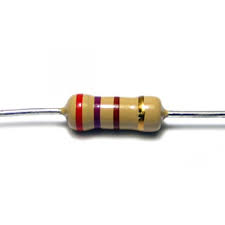
\includegraphics[width=0.5\textwidth]{figs/resistor1.jpg}
	\caption{Exemplo de resistor utilizado em circuitos eletr�nicos.}
	\label{resistor1}
\end{figure}

A simbologia para resitores num circuito el�trico � tamb�m extensa. A Figura \ref{resistor2} mostra todos os tipos de simbologia utilizado para v�rias aplica��es.

\begin{figure}[h]
	\centering
	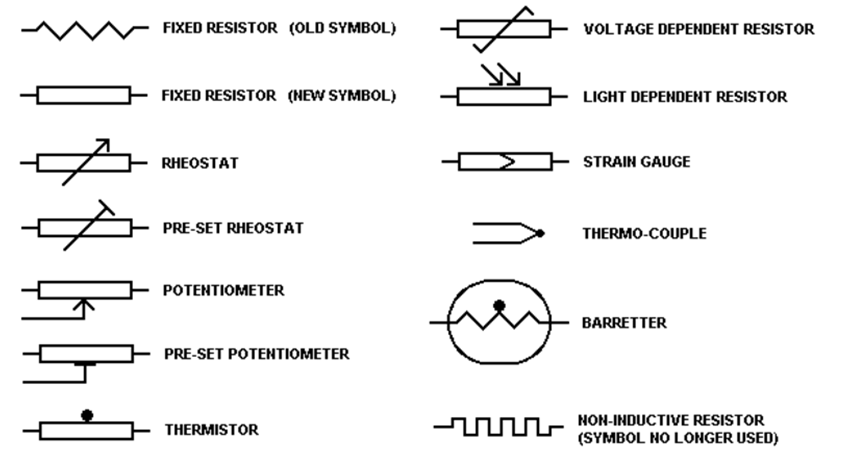
\includegraphics[width=0.6\textwidth]{figs/resistor2.png}
	\caption{Simbolos de resistor utilizado em circuitos eletr�nicos.}
	\label{resistor2}
	\source{www.vegyelgep.bme.hu}
\end{figure}

\begin{figure}[h]
	\centering
	\includegraphics[width=0.5\textwidth]{figs/resistor3.jpg}
	\caption{Como ler o c�dido de cores de um resistor.}
	\label{resistor3}
	\source{http://education.rec.ri.cmu.edu/content/electronics/common/resistors/1.html}
\end{figure}

Resistores de valor fixo, como o mostrado na Figura \ref{resistor3}, tem como resist�ncia a seguinte express�o: 	

\begin{equation}\label{eqResistenciaTabela}
R = (Digito_{1} + 10*Digito_{2})*Multiplicador \pm Tolerancia \% 
\end{equation}

Os valores \textit{$Digito_{1}$ , $Digito_{2}$, Multiplicador e Toler�ncia} s�o mostrados na Tabela \ref{tabCores} para cada cor utilizada no c�digo.
% Please add the following required packages to your document preamble:
% \usepackage[table,xcdraw]{xcolor}
% If you use beamer only pass "xcolor=table" option, i.e. \documentclass[xcolor=table]{beamer}
\begin{table}[]
	\centering
	\caption{Tabela de leitura de valor e toler�ncia de um resistor}
	\label{tabCores}
	\begin{tabular}{|c|c|c|l|c|}
		\hline
		Cor                             & Multiplicador                 & D�gito 1                 & Digito 2                 & {\color[HTML]{333333} Toler�ncia} \\ \hline
		\rowcolor[HTML]{000000} 
		{\color[HTML]{FFFFFF} Preto}    & {\color[HTML]{FFFFFF} $10^0$} & {\color[HTML]{FFFFFF} 0} & {\color[HTML]{FFFFFF} 0} & {\color[HTML]{333333} }           \\ \hline
		\rowcolor[HTML]{643403} 
		{\color[HTML]{FFFFFF} Marrom}   & {\color[HTML]{FFFFFF} $10^1$} & {\color[HTML]{FFFFFF} 1} & {\color[HTML]{FFFFFF} 1} & {\color[HTML]{FFFFFF} $\pm1\%$}   \\ \hline
		\rowcolor[HTML]{FE0000} 
		{\color[HTML]{FFFFFF} Vermelho} & {\color[HTML]{FFFFFF} $10^2$} & {\color[HTML]{FFFFFF} 2} & {\color[HTML]{FFFFFF} 2} & {\color[HTML]{FFFFFF} $\pm2\%$}   \\ \hline
		\rowcolor[HTML]{F56B00} 
		Laranja                         & $10^3$                        & 3                        & 3                        & {\color[HTML]{333333} }           \\ \hline
		\rowcolor[HTML]{FCFF2F} 
		{\color[HTML]{000000} Amarelo}  & {\color[HTML]{000000} $10^4$} & 4                        & 4                        & {\color[HTML]{333333} }           \\ \hline
		\rowcolor[HTML]{34FF34} 
		{\color[HTML]{FFFFFF} Verde}    & {\color[HTML]{FFFFFF} $10^5$} & 5                        & 5                        & {\color[HTML]{333333} }           \\ \hline
		\rowcolor[HTML]{3531FF} 
		{\color[HTML]{FFFFFF} Azul}     & {\color[HTML]{FFFFFF} $10^6$} & 6                        & 6                        & {\color[HTML]{333333} }           \\ \hline
		\rowcolor[HTML]{6200C9} 
		{\color[HTML]{FFFFFF} Violeta}  & {\color[HTML]{FFFFFF} $10^7$} & 7                        & 7                        & {\color[HTML]{333333} }           \\ \hline
		\rowcolor[HTML]{C0C0C0} 
		{\color[HTML]{FFFFFF} Cinza}    & {\color[HTML]{FFFFFF} $10^8$} & 8                        & 8                        & {\color[HTML]{333333} }           \\ \hline
		Branco                          & $10^9$                        & 9                        & 9                        & {\color[HTML]{333333} }           \\ \hline
		\rowcolor[HTML]{FFCB2F} 
		Ouro                            &                               &                          &                          & {\color[HTML]{333333} $\pm5\%$}   \\ \hline
		\rowcolor[HTML]{C0C0C0} 
		Prata                           &                               &                          &                          & {\color[HTML]{333333} $\pm10\%$}  \\ \hline
	\end{tabular}
\end{table}

Cada resistor tem um limite que corrente que pode circular entre seus terminais. Geralmente esse limite � dado em rela��o � pot�ncia dissipada. Para saber qual pot�ncia ser� dissipada num resistor com resist�ncia de valor \textit{R Ohms} deve-se aplicar a seguinte f�rmula:

\begin{equation}\label{eqPotencia}
\begin{split}
P = IU \text{(Pot�ncia dissipada num resistor de valor R)}
\end{split}
\end{equation}

Onde \textit{P} � a pot�ncia dissipada em \textit{Watts}, I � a corrente el�trica que passa no resistor em \textit{Amp�res} e \textit{U} � a tens�o el�trica entre os terminais do resistor em \textit{Volts}.


 


\subsection{Circuito - f�rmulas e topologias b�sicas}
\label{EmbassamentoHardware_circuito}

Nomea-se por circuito el�trico, um caminho fechado entre dois ou mais pontos formado por componentes eletr�nicos no qual corrente el�trica pode circular. A Figura \ref{circuito1} mostra um circuito el�trico simples formado por uma bateria que fornece uma diferen�a de potencial (Tens�o) entre seus terminais de valor \textit{\textbf{V} Volts} e um resistor com valor de resist�ncia \textbf{\textit{R} Ohms}. 

Os pontos A e B da figura mostram, respectivamente, o ponto de maior potencial el�trico ( + da bateria) e o ponto de menor potencial el�trico (- da bateria).

 Para descrever o comportamento a din�mica de tens�es, correntes existem as seguintes leis:

\begin{itemize}
	\item Primeira lei de Kirchoff - Leis das Malhas
	\item Segunda lei de Kirchoff - Leis dos N�s
	\item Lei de Ohm
\end{itemize}

E para descrever a topologia dos circuitos, existem duas liga��es b�sicas entre componentes a serem tradadas neste documento:

\begin{itemize}
	\item Liga��o S�rie
	\item Liga��o Paralelo
\end{itemize}


\begin{figure}[h]
	\centering
	\includegraphics[width=0.5\textwidth]{figs/circuito1.png}
	\caption{Circuito Simples.}
	\label{circuito1}
\end{figure}

\subsubsection{Primeira lei de Kirchoff - Leis das N�s}
\label{lei1Kirchoff}
A primeira lei de Kirchoff diz que a soma da correntes el�tricas que entram num n� $I_{entram} $� igual a soma das correntes que saem, $ I_{saem}$, ou seja:
\begin{equation}\label{eqKirchoof1}
\sum I_{entram} = \sum I_{saem}
\end{equation}

Usando a Figura \ref{circuito3} como exemplo, a primeira, nesse caso, � escrita da seguinte forma:

\begin{equation}\label{eqKirchoof11}
 I_{1} + I_{3} = I_{2} + I_{4} + I_{5}
\end{equation}

\begin{figure}[h]
	\centering
	\includegraphics[width=0.5\textwidth]{figs/circuito3.jpg}
	\caption{Primeira Lei de Kirchoff.}
	\label{circuito3}
\end{figure}


\subsubsection{Segunda lei de Kirchoff - Leis das Malhas}
\label{lei2Kirchoff}
A segunda lei de Kirchoff diz que a soma das tens�es $u_{i}$ num caminho fechado, num circuito el�trico � igual a zero, ou seja:

\begin{equation}\label{eqKirchoof2}
\sum u_{i} = 0
\end{equation}

Usando a Figura \ref{circuito2} como exemplo, onde as tens�o em cada componentes s�o descritas pela letra \textbf{\textit{u}} ,a primeira lei Kirchoff � escrita na seguinte forma

\begin{figure}[h]
	\centering
	\includegraphics[width=0.5\textwidth]{figs/circuito2.png}
	\caption{Segunda Lei Kirchhoff.}
	\label{circuito2}
\end{figure}

\begin{equation}\label{eqKirchoof22}
\begin{split}
u - u_{1} - u_{2} = 0 \\
u = u_{1} + u_{2}
\end{split}
\end{equation}


\subsubsection{Lei de Ohm}
\label{leiOhm}

A lei de Ohm\cite{livro:Sedra} diz que num circuito fechado, sob um componente eletr�nico que com valor resist�ncia \textit{R} que esteja submetido a uma diferen�a de potencial entre seus terminais de valor \textit{V}, circular� uma corrente el�trica de \textit{I} segundo a seguinte f�rmula:
\begin{equation}
I = \frac{V}{R}
\end{equation}

Essa express�o n�o depende da natureza de tal condutor: ela � v�lida para todos os condutores. Para um dispositivo condutor que obede�a � lei de Ohm, a diferen�a de potencial aplicada � proporcional � corrente el�trica, isto �, a resist�ncia � independente da diferen�a de potencial e da corrente. Um dispositivo muito utilizado em aparelhos eletr�nicos, como r�dios, televisores e amplificadores, que obedece � essa lei � o resistor (componente descrito mais detalhadamente na se��o \ref{Embassamento_resitor}) cuja fun��o � controlar a intensidade de corrente el�trica que passa pelo aparelho.

Entretanto, para alguns materiais, por exemplo os semicondutores, a resist�ncia el�trica n�o � constante, mesmo que a temperatura seja, ela depende da diferen�a de potencial V. Estes s�o denominados condutores n�o �hmicos. Um exemplo de componente eletr�nico que n�o obedece � lei de Ohm � o diodo(componente descrito mais detalhadamente na se��o \ref{Embassamento_LED}).

\subsubsection{Liga��o em S�rie}
\label{ligacaoSerie}
Quando dois ou mais componentes est�o conectados num circuito, um ap�s ao outro, diz que tais componentes est�o conectados em s�rie, como mostrado em \ref{circuito4}. 


\begin{figure}[h]
	\centering
	\includegraphics[width=0.5\textwidth]{figs/circuito4.png}
	\caption{Liga��o em s�rie de n resistores.}
	\label{circuito4}
\end{figure}

Para elementos que se encontram em s�rie, a mesma corrente \textit{I} os percorre, como mostrado na Figura \ref{circuito5}.

\begin{figure}[h]
	\centering
	\includegraphics[width=0.5\textwidth]{figs/circuito5.png}
	\caption{Mesma corrente percorrendo resistores em s�rie.}
	\label{circuito5}
\end{figure}

Aplicando a segunda lei de Kirchoff, apresentada na se��o \ref{lei2Kirchoff}, e a lei de Ohm, apresentada na se��o \ref{leiOhm}, tem-se a seguinte sequ�ncia de express�es para a demonstra��o da resist�ncia equivalente de resistores em s�rie: 


\begin{equation}\label{eqSerie1}
\begin{split}
V_{+} - V_{-} = V_{R1} + V_{R2} + ... V_{Rn}   \quad \text{(Aplicando a lei de Kirchoff das malhas)}
\end{split}
\end{equation}


\begin{equation}\label{eqSerie2}
\begin{split}
I*R_{eq} = I*(R1 + R2 + ... Rn )   \quad \text{( Aplicando a Lei de Ohm)}
\end{split}
\end{equation}


\begin{equation}\label{eqSerie3}
\begin{split}
R_{eq} = (R1 + R2 + ... Rn )   \quad \text{( F�rmula de resistor equivalente - liga��o s�rie)}
\end{split}
\end{equation}

A resist�ncia equivalente de uma liga��o em s�rie de resistores pode ser vista como a "resist�ncia enxergada" pela fonte de diferen�a de potencial entre os pontos V+ e V- mostrados na Figura \ref{circuito5}.



\subsubsection{Liga��o em Paralelo}
\label{ligacaoParalelo}
Numa conex�o em paralelo, os componentes se encontram conectados com seus terminais conectados em comum e possuem sobre eles a mesma tens�o el�trica, como mostrado na Figura \ref{circuito6}.

A primeira lei de Kirchoff, como mostrado na se��o \ref{lei1Kirchoff}, mostra que a soma das correntes que entram num n� � igual a soma das correntes que por ele saem. 

Na Figura \ref{circuito6}, os resistores $R_{1}$, $R_{2}$,...$R_{n}$ encontram em paralelo. A soma das correntes que entram no n� A e igual a soma das correntes que dele saem, ou seja: 

\begin{equation}\label{eqParalelo1}
\begin{split}
I = I_{1} + I_{2} + ... +I_{n}  \quad \text{(Primeira Lei de Kirchoff)}
\end{split}
\end{equation}

Utilizando a Lei de Ohm e sabendo que, numa liga��o em paralelo, todos elementos encontram-se sob a mesma Tens�o el�trica, tem-se que:

\begin{equation}\label{eqParalelo2}
\begin{split}
\frac{V_{in}}{R_{eq}} = \frac{V_{in}}{R_{1}} + \frac{V_{in}}{R_{2}} + ... \frac{V_{in}}{R_{n}}  \quad \text{(Lei de Ohm aplicada � liga��o em paralelo)}
\end{split}
\end{equation}

Disso, tem -se que:

\begin{equation}\label{eqSerie3}
\begin{split}
\frac{1}{R_{eq}} = \frac{1}{R_{1}} + \frac{1}{R_{2}} + ... \frac{1}{R_{n}}  \quad \text{( F�rmula de resistor equivalente - liga��o paralelo)}
\end{split}
\end{equation}


\begin{figure}[h]
	\centering
	\includegraphics[width=0.5\textwidth]{figs/circuito6.png}
	\caption{Componentes conectados em paralelo.}
	\label{circuito6}
\end{figure}

\subsubsection{Resumo - Liga��o em s�rie X paralelo}
\label{ResumoSerieEParalelo}

A tabela mostrada em \ref{tabResumoSerieParaleo} o resumo das caracter�stica da liga��o em s�rie e da liga��o em paralelo entre resistores:

\begin{table}[]
	\centering
	\caption{Resumo - Liga��o em s�rie X Liga��o em paralelo}
	\label{tabResumoSerieParaleo}
	\begin{tabular}{l|l|l|l|}
		\cline{2-4}
		& \textbf{\begin{tabular}[c]{@{}l@{}}Tens�o el�trica\\  nos elementos\end{tabular}} & \textbf{\begin{tabular}[c]{@{}l@{}}Corrente el�trica \\ pelos elementos\end{tabular}} & \textbf{\begin{tabular}[c]{@{}l@{}}Resist�ncia Equivalente entre\\ N elementos conectados\end{tabular}} \\ \hline
		\multicolumn{1}{|l|}{\textbf{Liga��o em S�rie}}    & Diferente                                                                         & Igual                                                                                 & $R_{eq} = R_{1} + R_{2} + ... + R_{n}$                                                                  \\ \hline
		\multicolumn{1}{|l|}{\textbf{Liga��o em Paralelo}} & Igual                                                                             & Diferente                                                                             & $\frac{1}{R_{eq}} = \frac{1}{R_{1}} + \frac{1}{R_{2}} + ... \frac{1}{R_{n}}$                            \\ \hline
	\end{tabular}
\end{table}


\subsection{Diodo-LED}
\label{EmbassamentoHardware_LED}


Um \textbf{Diodo Emissor de Luz} (LED) � um dispositivo semicondutor o qual, ao passar de corrente el�trica do seu \textit{�nodo} para seu \textit{C�todo} emite luz. A Figura \ref{LED1} mostra o s�mbolo de um LED.

Como todo diodo, o LED bloqueia a passagem de corrente el�trica na dire��o do seu c�todo ao seu �nodo e permite a passagem de corrente na dire��o contr�ria.

Como mostrado na Figira \ref{LED0}, diodo s�o constru�dos com duas jun��es de semicondutores dopados: uma jun��o N e uma jun��o P. A jun��o P possui falta de portadores negativos, ou seja, est� positivamente dopado. A jun��o N possui excesso de portadores negativos, ou seja, est� negativamente dopada. 

A din�mica dos portadores entre as jun��es N - P criem o comportamento de bloqueio e libera��o da passagem de corrente no diodo. 

Para um diodo com tens�o positiva entre �nodo e c�todo, existe uma regi�o chamada regi�o de deple��o a qual deve ser superada para que exista fluxo de corrente, ainda que o diodo esteja positivamente polarizado, como mostrado tamb�m no gr�fico da Figura \ref{LED2}.

\begin{figure}[H]
	\centering
	\includegraphics[width= 1\textwidth]{figs/LED0.png}
	\caption{Jun��o N-P em um diodo.}
	\label{LED0}
\end{figure}


\begin{figure}[H]
	\centering
	\includegraphics[width=0.5\textwidth]{figs/diodo1.png}
	\caption{S�mbolo Diodo}
	\label{LED1}
\end{figure}

A  Figura \ref{LED2} mostra a rela��o entre tens�o aplicada entre o �nodo e o c�todo e a corrente que atravessa um diodo. Quando a diferen�a de tens�o entre �nodo e c�todo � positiva, o diodo se encontra sob polariza��o direta. Nessa polariza��o, o diodo permite passagem de corrente entre seus terminais. A f�rmula que expressa essa rela��o � a seguinte:


\begin{equation}\label{eqDiodo1}
\begin{split}
i_{D} = I_{s}(e^{v_{d}/nkT} - 1) 
\end{split}
\end{equation}

Onde $i_{D}$ � a corrente se passar pelo diodo, $v_{D}$ � a tens�o entre �nodo e c�todo, T � a temperatura, k � a constante de Boltzmann, N � o coeficiente de n�o linearidade e $I_{s}$ � a corrente de satura��o.

Como mostrado na Figura \ref{LED2}, quando em polariza��o reversa, o diodo n�o permite passagem de corrente com intensidade apreci�vel. 

Caso a diferen�a de tens�o entre c�todo e �nodo seja maior que a tens�o de quebra $V_{br}$, o diodo entrar� na regi�o de quebra e n�o mais bloquear� a passagem de corrente.


\begin{figure}[H]
	\centering
	\includegraphics[width=1\textwidth]{figs/LED2.png}
	\caption{Rela��o tens�o, corrente num diodo e suas regi�es de opera��o}
	\label{LED2}
	\source{$http://www2.feg.unesp.br/Home/PaginasPessoais/ProfMarceloWendling/2---diodo-semicondutor.pdf$}
\end{figure}

Para aplica��es simples em eletr�nica, usualmente se adota um modelo simplificado para a opera��o do diodo mostrado na Figura \ref{LED3}. 

Nesse modelo, para uma polariza��o direta, o diodo � substitu�do por um diodo ideal (sem queda de tens�o) com uma bateria em s�rie com valor de tens�o de 0.7 a 0.6 de tens�o significando a queda de tens�o entre os terminais do diodo. 

\begin{figure}[H]
	\centering
	\includegraphics[width=1\textwidth]{figs/LED3.jpg}
	\caption{Modelo simplificado de um diodo em polariza��o direta.}
	\label{LED3}
	\source{https://digitalsignal.files.wordpress.com/2008/09/aula05.pdf}
\end{figure}

Diodo s�o utilizados em v�rias aplica��es em eletr�nica. Alguns exemplo de aplica��es seriam:

\begin{itemize}
	\item Retifica��o de tens�o (Transforma��o de um sinal AC (Corrente Alternada) para DC (Corrente Cont�nua))
	\item Isolamento de sinais de fonte de pot�ncia
	\item Refer�ncia de voltagem
	\item Controle e limita��o da amplitude de sinais
	\item Detec��o de sinais
\end{itemize}

\subsection{Protoboard}
\label{EmbassamentoHardware_Protoboard}

Protoboard ou \textit{BreadBoard} � um componente essencial na prototipa��o de circuitos eletr�nicos. Com uma protoboard, � poss�vel criar circuitos tempor�rios, sem necessidade de realizar soldagem. 

As protoboards foram criadas para simplificar a prototipa��o e testes de circuitos eletr�nicos anteriormente a sua efetiva produ��o por meio em m�quinas de circuitos impress
Em geral, as protoboards apresentam a estrutura mostrada na Figura \ref{protoboard1}. As trilhas verticais + e - marcadas na Figura s�o trilhas cont�nuas de alum�nio. Usualmente, mas n�o obrigatoriamente, as trilhas + e - s�o usadas como para os polos positivo e negativo da bateria. A regi�o central, com as trilhas na horizontal, geramente � utilizada para a constru��o do circuito desejado.

\begin{figure}[H]
	\centering
	\includegraphics[width=0.5\textwidth]{figs/protoboard1.jpg}
	\caption{Protoboard.}
	\label{protoboard1}
	\source{https://learn.sparkfun.com/tutorials/how-to-use-a-breadboard}
\end{figure}

A Figura \ref{protoboard3} mostra o esquem�tico de circuito simples formado por uma fonte de 9V, uma resistor de 1k ohm e um LED e sua constru��o numa protoboard.

Na parte direita da Figura \ref{protoboard3}, � mostrado os polos positivo e negativos da bateria de 9V conectado � trilha cont�nua e a regi�o central foi usada para conectar tais polos ao LED e resistor em s�rie. Al�m disso, a parte direita da Figura mostra o sentido convencional da corrente el�trica. 

\begin{figure}[H]
	\centering
	\includegraphics[width=1\textwidth]{figs/protoboard3.jpg}
	\caption{Esquem�tico de um circuito e sua constru��o numa protoboard.}
	\label{protoboard3}
\end{figure}




\subsection{Divisor de tens�o}
\label{EmbassamentoHardware_DivisorTesao}

Em eletr�nica, chama-se divisor de tens�o um circuito com estrutura similar ao mostrada na Figura \ref{divisorTensao1}.

\begin{figure}[H]
	\centering
	\includegraphics[width=0.5\textwidth]{figs/divisor1.png}
	\caption{Modelo de um circuito divisor de tens�o}
	\label{divisorTensao1}
\end{figure}

Pela segunda lei de Kirchoff (se��o \ref{lei2Kirchoff}) tem-se a seguinte express�o:

\begin{equation}\label{eqDivisorTensao1}
\begin{split}
V_{in} - V_{R1} - V_{R2} = 0
\end{split}
\end{equation}



A corrente que circular� nesse circuito � igual a: 

\begin{equation}\label{eqDivisorTensao2}
\begin{split}
I = \frac{V_{in}}{(R1 + R2)}
\end{split}
\end{equation}

Calculando o valor da tens�o de sa�da, tem-se:

\begin{equation}\label{eqDivisorTensao3}
\begin{split}
V_{out} = V_{in} - I*R1
\end{split}
\end{equation}

Portanto, a tens�o de sa�da ser� igual a:


\begin{equation}\label{eqDivisorTensao4}
\begin{split}
V_{out} = \frac{R2}{R1 + R2} * V_{in} 
\end{split}
\end{equation}


O fator $\frac{R2}{R1 + R2}$ � o fator da divis�o de tens�o, no circuito exemplificado pela Figura \ref{divisorTensao1}.

Divisores de tens�o tem v�rias aplica��es em eletr�nica, dentre elas, destacam-se as seguintes:

\begin{itemize}
	\item \textbf{Medi��o de sensores}: Um divisor de tens�o pode ser usado como forma de medi��o para sensores resistivos ( Sensores que alteram sua resist�ncia de acordo com o fator de sensitividade). 
	
	\item \textbf{Medi��o de altas tens�es}: Um divisor de tens�o pode ser usado para utilizar volt�metros para tens�es al�m de sua respectivas escala de medi��o.
	
	\item \textbf{Mudan�a de escala de sinais}: Um divisor de tens�o pode ser usado para adeguar a escala de um sinal para sinais que podem ser lidos e processados por um microprocessador em suas faixa opera��o pr�pria.

\end{itemize}

\subsection{Potenci�metro}
\label{EmbassamentoHardware_Potenciometro}
Um potenci�metro � um componente de circuitos el�tricos que possui resist�ncia el�trica ajust�vel mecanicamente. Num esquem�tico de um circuito, o s�mbolo usado para potenci�metro � mostrado na Figura \ref{potenciometro1}.

\begin{figure}[H]
	\centering
	\includegraphics[width=0.5\textwidth]{figs/potenciometro1.png}
	\caption{S�mbolo de um potenci�metro.}
	\label{potenciometro1}
\end{figure}

Potenci�metros s�o muito usados para controlar / alterar as caracter�sticas de entrada / sa�da de aparelhos eletr�nicos, como volume, balan�o, graves, brilho, contraste, cor, tempo de funcionamento (em tv's, dvd's, monitores, rel�gios, ... ).S�o tamb�m conhecidos como resistores vari�veis, ou ainda, reostatos.

Para criar tal caracter�stica de varia��o de resist�ncia, os pot�nciometros possuem internamente uma trilha resistiva (de n�quel-cromo ou de carbono), sobre a qual desliza um  cursor , que altera a resist�ncia el�trica entre seu conector central e um dos dois laterais(normalmente s�o tr�s conectores).

Os potenci�metros podem ser classificados em duas categorias: quanto a forma de deslocamento do curso e quanto a forma de varia��o da resist�ncias entre seus terminais.

Em rela��o a forma de deslizamento do curso, os potenci�metros podem ser angulares, Figura \ref{potenciometro2}, e lineares, Figura \ref{potenciometro4}.

\begin{figure}[H]
	\centering
	\includegraphics[width=0.5\textwidth]{figs/potenciometro2.png}
	\caption{Estrutura de um potenci�metro angular.}
	\label{potenciometro2}
\end{figure}


\begin{figure}[H]
	\centering
	\includegraphics[width=0.5\textwidth]{figs/potenciometro4.jpg}
	\caption{Potenci�metro linear.}
	\label{potenciometro4}
\end{figure}

Em rela��o a a forma de varia��o da resist�ncia entre seus terminais, os pot�nciometros podem ter varia��o linear ou varia��o logar�timica. A Figura \ref{potenciometro5} mostra tais formas de varia��o.


\begin{figure}[H]
	\centering
	\includegraphics[width=0.5\textwidth]{figs/potenciometro5.jpg}
	\caption{Formas de varia��o da resist�ncia em um pot�nciometro.}
	\label{potenciometro5}
\end{figure}

Assumindo que a resist�ncia entreos terminais externos do pot�ncioemtro da Figura \ref{potenciometro3} � fixa e igual a 10 k ohms tem-se as seguintes formas de uso dos terminais:

\begin{itemize}
	\item \textbf{Ponteci�metro 1}: est� com os terminais 1 e 2 ligados, neste caso ele varia sua resist�ncia entre 0 ohm e 10 k ohms, nessa liga��o quando o eixo � girado para a esquerda ele diminui a sua resist�ncia e quando ele � girado  para a direita aumenta a sua resist�ncia.
	\item \textbf{Ponteci�metro 2}: Nesse caso,os terminais 2 e 3 encontram-se ligados, ele varia sua resist�ncia entre 0 ohm e 10 k ohms, nessa liga��o quando o eixo � girado para a esquerda ele aumenta a sua resist�ncia e quando � girado para a direita diminui a sua resist�ncia.
	\item \textbf{Ponteci�metro 3}: a resist�ncia � fixa, no caso 10 k ohms. Girar o curso n�o alterar� a resist�ncia observada.
	 
\end{itemize}



\begin{figure}[H]
	\centering
	\includegraphics[width=0.5\textwidth]{figs/potenciometro3.png}
	\caption{Formas de uso de um pot�nciometro angular. }
	\label{potenciometro3}
\end{figure}

Um exemplo de utiliza��o de potenci�metros s�o os \textit{joysticks} utilizados em jogos eletr�nicos. A Figura \ref{potenciometro7} mostra um circuito integrado de um joystick. 

O joystick mostrado � implementado utilizando dois potenci�metros. Um dos potenci�metros � traduz em tens�o a posi��o X em rela��o � posi��o inicial e o outro traduz a posi��o Y.

\begin{figure}[H]
	\centering
	\includegraphics[width=0.5\textwidth]{figs/potenciometro7.jpg}
	\caption{Circuito integrado de um joystick que utiliza dois potenci�metros para tradu��o de sua posi��o em tens�o. }
	\label{potenciometro7}
\end{figure}

A Figura \ref{potenciometro6} mostra um circuito esquem�tico utilizando um joystick constru�do com 2 potenci�metros.

\begin{figure}[H]
	\centering
	\includegraphics[width=0.7\textwidth]{figs/potenciometro6.jpg}
	\caption{Circuito esquem�tico de um circuito utilizando um joystick similar ao mostrado na Figura \ref{potenciometro7} com a placa Galileo.}
	\label{potenciometro6}
\end{figure}

Para o circuito mostrado na Figura \ref{potenciometro6}, os potenci�metros est�o sob 5V de tens�o. Na posi��o inicial, ambas portas anal�gicas 0 e 1 ,que le�m as posi��es X e Y, ler�o 2.5 V. Ao se movimentar o joystick, as portas anal�gicas ler�o algum valor entre 0 e 5V.

\subsection{LDR}
\label{EmbassamentoHardware_LDR}

Um foto-resistor ou LDR (Light Dependent Resistor) � um resistor cuja resit�ncia � dependente da luz que incide sobre ele. A Figura \ref{ldr1} mostra um LDR simples, muito utilizado em circuitos eletr�nicos e a Figura \ref{ldr2} mostra a s�mbolo para o LDR usado em esquem�ticos.  

Resistores dependentes de luz podem ser de diferentes tipos. Eles variam em material sens�vel � luz usada. Um resistor dependente da luz no espectro vis�vel� feita atrav�s de sulfureto de c�dmio (CdS) ou seleneto de c�dmio (CdSe). Este material � sens�vel ao comprimento de onda de 400 nm - 850 nm. Por perto faixa do infravermelho (1 \si\micro m - 3 \si\micro m), existem PBS ou materiais PBSE usado. 


\begin{figure}[H]
	\centering
	\includegraphics[width=0.5\textwidth]{figs/ldr1.png}
	\caption{LDR}
	\label{ldr1}
\end{figure}


\begin{figure}[H]
	\centering
	\includegraphics[width=0.4\textwidth]{figs/ldr3.jpg}
	\caption{S�mbolo do LDR}
	\source{www.electrical4u.com}
	\label{ldr2}
\end{figure}

Um LDR pode de dezenas de Megaohms (Escuro) para algumas centenas de ohms (claro) dependendo da intensidade da luz incidente, como mostrado no gr�fico da Figura \ref{ldr3}.

\begin{figure}[H]
	\centering
	\includegraphics[width=0.5\textwidth]{figs/ldr2.jpg}
	\caption{Gr�fico LDR : Resist�ncia X Lumin�ncia}
	\source{www.electrical4u.com}
	\label{ldr3}
\end{figure}


Como dito na se��o \ref{EmbassamentoHardware_DivisorTesao}, um divisor de tens�o pode ser usado em conjunto com sensores resistivos como o LDR. A Figura \ref{ldr4} mostra um sensor de luz implementado com um circuito formado por uma fonte DC, um resistor fixo de 10k ohms e um LDR.


\begin{figure}[H]
	\centering
	\includegraphics[width=0.5\textwidth]{figs/ldr4.jpg}
	\caption{Poss�vel circuito a ser utilizado num sensor de luz}
	\label{ldr4}
\end{figure}

 A tens�o de sa�da \textit{Vout} � dada segundo a seguinte express�o: 
 
 \begin{equation}\label{eqLDR}
 \begin{split}
 V_{out} = \frac{10k}{10k + R_{LDR}} * 5 
 \end{split}
 \end{equation}
 
 Onde $R_{LDR}$ obedece ao gr�fico mostrado na Figura \ref{ldr3}.

\subsection{Interruptores}
\label{interruptores}
Ao se desenvolver circuitos eletr�nicos, existem duas express�es muita comuns: circuito aberto e circuito fechado. 

Um circuito aberto � mostrado na Figura \ref{interruptor1}. Nesse circuito, corrente alguma sai da fonte e passa pela l�mpada.

 Pode-se dizer que a regi�o entre A e B � uma resistor com resist�ncia que tende ao infinito. Usando essa suposi��o, ao se calcular a corrente que circula numa regi�o de circuito aberto tem-se a seguinte express�o:

\begin{equation}\label{eqCircuitoAberto}
 \begin{split}
 I = \lim_{R_{AB}\to\infty} \frac{V_{bateria}}{R_{lampada} + R_{AB}} = 0 A 
 \end{split}
\end{equation}

\begin{figure}[H]
	\centering
	\includegraphics[width=0.5\textwidth]{figs/interruptor1.jpg}
	\caption{Circuito aberto.}
	\label{interruptor1}
\end{figure}


Um circuito fechado, � um circuito que se encontra caminho efetivo, para passagem de corrente el�trica. Na Figura \ref{interruptor2} � mostrado o mesmo circuito da Figura \ref{interruptor1} fechado.


\begin{figure}[H]
	\centering
	\includegraphics[width=0.5\textwidth]{figs/interruptor2.jpg}
	\caption{Circuito fechado.}
	\label{interruptor2}
\end{figure}


Abrir ou fechar uma regi�o de um circuito ou ele por completo pode-ser feito utilizando interruptores ou chaves.

Interruptores ou chaves tem por prop�sito abrir ou fechar um circuito ou certa regi�o de um circuito de acordo com a vontade de um agente externo. A Figura \ref{interruptor3} mostra o s�mbolo de um interruptor num circuito el�trico.


\begin{figure}[H]
	\centering
	\includegraphics[width=0.5\textwidth]{figs/interruptor3.jpg}
	\caption{S�mbolo de um interruptor.}
	\label{interruptor3}
\end{figure}

Um tipo especial de interruptor � o bot�o. A Figura \ref{interruptor4} mostra a imagem e esquem�tico de mini bot�es. 

Os Mini Push Buttons s�o tamb�m chamados de interruptores tendenciosos ou moment�neos, porque ap�s precionados, eles retornam ao estado de origem (aberto ou fechado).

Existem 2 tipos de Mini Bot�es de Press�o quanto ao seu estado:

\begin{itemize}
	\item NO (abrevia��o de Normally Open), esse interruptor moment�neo fica normalmente aberto (desligado), mas quando pressionado e segurado o bot�o, o interruptor fecha (liga). Ao soltar o bot�o, o interruptor abre novamente. Utilizado em teclados de computadores, calculadoras, etc.

\item NC (abrevia��o de Normally Closed), esse interruptor moment�neo fica normalmente fechado (ligado), mas quando apertado e segurado o bot�o, o interruptor abre (desliga). Ao soltar o bot�o, o interruptor fecha novamente. Utilizado na ilumina��o interna das geladeiras, ve�culos, etc. (ao abrir a porta, o interruptor � acionado, fechando o circuito). 
\end{itemize}

\begin{figure}[H]
	\centering
	\includegraphics[width=0.8\textwidth]{figs/interruptor4.jpg}
	\caption{Mini bot�es de press�o, de 2 e 4 pinos.}
	\label{interruptor4}
	\source{$http://www.dreaminc.com.br/sala_de_aula/9b-interruptores-mini-botao-de-pressao/$}
\end{figure}

O mini bot�o de 4 pinos de contato � muitas vezes utilizado para oferecer tens�o alta (HIGH) e baixa (LOW) para uma porta de uma placa como a placa Galileo.

\begin{figure}[H]
	\centering
	\includegraphics[width=0.8\textwidth]{figs/interruptor5.jpg}
	\caption{Circuito simples utilizando um bot�o de 4 pinos de contato .}
	\label{interruptor5}
\end{figure}

A Figura \ref{interruptor5} mostra um exemplo de um circuito constru�do em conjunto com a placa Galileo. Nesse circuito, a porta digital 2 pode ler um n�vel de tens�o alta (HIGH) ou baixa(LOW) dependendo do bot�o estar pressionado ou n�o. Como mostrado no esquem�tico, quando o bot�o � pressionado, os ponto A e B se encostam e na porta digital passa a existir a tens�o alta.

As aplica��es para bot�es em eletr�nica s�o diversas. Neste trabalho, muitas pr�ticas usar�o bot�es no seu desenvolvimento.

\subsection{Registrador de deslocamento (Shift Register)}
\label{shift}
Registadores de deslocamento s�o muito utilizados na convers�o entre interfaces seriais para interfaces paralelas. A Figura \ref{shift1} mostra um resumo do funcionamento de um registrador de deslocamento. 

\begin{figure}[H]
		\centering
	\includegraphics[width=0.8\textwidth]{figs/shift1.jpg}
	\caption{Esquema resumido: S�rie para Paralelo com um registrador de deslocamento.}
	\label{shift1}
	\source{Adaptado de http://electriciantraining.tpub.com/14185/css/Serial-And-Parallel-Transfers-And-Conversion-Continued-151.htm}
\end{figure}

Cada bit que chega no registrador de deslocamento � escrito nas portas paralelas seguencialmente. 

Tal comportamento � realizado por meio de uma cascata de \textit{flip-flops}. Um flip-flop � um dispositivo que armazena ou reseta um bit de acordo com sinais nas suas portas. 

A figura \ref{shift2} mostra a estrutura interna de um registrador de deslocamento com mais detalhes. Cada vez que um salto alto � posto no pino de Clock, um novo bit que entra no pino \textit{Data in} e os que estavam armazenados nos \textit{flip-flops} s�o levados para os flip-flops da frente.

Os pinos Q1, Q2, Q3,...,QN s�o os pinos a serem utilizados para leitura paralela. 
\begin{figure}[H]
	\centering
	\includegraphics[width=0.8\textwidth]{figs/shift2.png}
	\caption{Cascata de \textit{flip-flops} num registrador de deslocamento.}
	\label{shift2}
\end{figure}

Uma arquitetura similar pode ser usada para realizar a convers�o entre comunica��o paralela para serial.

Registradores de deslocamento s�o muito utilizada para controlar diversas entradas e sa�das para al�m das entradas e sa�das disponibilizadas por um microcontrolador. 

Geralmente, os registradores de deslocamento tratam apenas de valores digitais($V_{cc} ou GND$) em seus pinos.

Para os prop�sitos deste trabalho, ser� usado o registrador de deslocamento 74HC595 \cite{DATASHEET3}. A Figura \ref{shift3} mostra a pinagem desse circuito integrado:

\begin{figure}[H]
	\centering
	\includegraphics[width=0.8\textwidth]{figs/shift3.jpg}
	\caption{Pinagem Registrador de Deslocamento 74HC595.}
	\label{shift3}
\end{figure}

A descri��o dos pinos � a seguinte:

\begin{itemize}
	\item\textbf{Pino 14}: Pino para entrada de dados seriais.
	\item \textbf{Pino 16}: Pino de alimenta��o VCC.
	\item \textbf{Pino 8}: Pino de refer�ncia GND.
	\item\textbf{Pinos 1 a 7 e 15 (Q1 a Q7 e Q0)}:
	\item \textbf{Pino 10:} O pino 10 � chamado de \textit{Master Reset (MR)}. Quando um valor baixo de tens�o � identificado nesse pino, o registrador de deslocamento � resetado e todos dados que ainda estiverem nele s�o perdidos.
	\item \textbf{Pino 11}: O pino 11 � destinado para o sinal do clock do sistema, que determinar� qual ser� a frequ�ncia com que os bits s�o deslocados pelo registrador.
	\item \textbf{Pino 12}: O pino 12 � o \textit{Latch Pin}. Quando este pino est� no estado de LOW, o registrador de deslocamento est� pronto para receber dados na sua pino de entrada. Quando este pino est� no estado de HIGH, o registrador de deslocamento � configurado para escrever os dados lidos no pinos Q1 a Q7 e Q0.
	\item \textbf{Pino 13}: O pino 13 � o pino respons�vel por permitir ou bloquear a transmiss�o dos dados para as portas de sa�da. Quando o pino est� no estado LOW (GND), a transmiss�o est� permitida, quando est� em estado HIGH, a transmiss�o est� bloqueada.
	 
\end{itemize}


Os bits que entram no pino 14 de forma serial e saem, como dito, sequencialmente nos pinos Q0, Q1, Q2, Q3, Q4, Q5, Q6 e Q7. 



\subsection{Sensor de Temperatura - LM35}
\label{sensorTemperatura}

Sensores de temperatura s�o dispositivos os quais possuem alguma propriedade mensur�vel alterada pela altera��o de temperatura.

Sensores s�o extremamente importantes para sistemas de automa��o, em qualquer escala ou ambiente.

Em industrias, onde h� processos de produ��o automatizados, temos muitos tipos de sensores medindo as mais diversas vari�veis do processo: temperatura, press�o, peso, pH, dentre muitos outros. Devido a import�ncia da leitura dessas vari�veis, existe uma �rea respons�vel por instrumentos de medi��o, a Instrumenta��o Industrial.

Em ambientes comerciais, sensores de temperatura s�o muito utilizados para controle de ar-condicionados e verifica��o de inc�ndios. Sensores de presen�a s�o importantes para seguran�a. 

Com rela��o a sensores de temperatura, um dos mais usados e baratos � o sensor LM35. O sensor LM35 possui as seguintes caracter�sticas:

\begin{itemize}
	\item Entrada temperatura, sa�da Tens�o el�trica: Alguns sensores de temperatura s�o sensores resistivos. Se esse fosse o caso, seria necess�rio a constru��o de um tipo de divisor de tens�o (se��o - \ref{EmbassamentoHardware_DivisorTesao}) para tratar com os dados do sensor na forma de tens�o de forma a ter uma vari�vel process�vel pela placa Galileo.
	\item Sem necessidade de calibra��o da escala Kelvin para Celsious: Muitas vezes, os sensores possuem respostas calibradas para a escala Kelvin, mas o LM35 j� � calibrado para Celsious. \textbf{A sensibilidade do LM35 � 10mV/$^{\circ}$C}
	\item O LM35 consome apenas 60  uA na faixa de 4 a 20 V de alimenta��o, portanto, pouca influ�ncia na leitura ocorre por auto-aquecimento\cite{DATASHEET4}.
\end{itemize} 	

A Figura \ref{lm35_0} mostra o LM35 e a Figura \ref{lm35_2} mostra sua pinagem.
\begin{figure}[H]
	\centering
	\includegraphics[width=0.4\textwidth]{figs/lm35.jpg}
	\caption{Sensor de Temperatura LM35.}
	\label{lm35_0}
\end{figure}

\begin{figure}[H]
	\centering
	\includegraphics[width=0.4\textwidth]{figs/lm35_2.jpg}
	\caption{Pinagem LM35.}
	\label{lm35_2}
\end{figure}

Na Figura \ref{lm35_2}, os pinos indicam o seguinte:

\begin{itemize}
	\item \textbf{+Vs}: Pino de alimenta��o. Para aplica��es com a placa Galileo, a alimenta��o 5V j� � adequada.
	\item \textbf{GND}: Pino para se conectado ao terra.
	\item \textbf{Vout}: Pino de sa�da da leitura realizada.
\end{itemize}

A Figura \ref{lm35_3} mostra a forma adequada de se conectar o LM35 � placa Galileo.
\begin{figure}[H]
	\centering
	\includegraphics[width=0.8\textwidth]{figs/lm35_3.jpg}
	\caption{Circuito sensor de temperatura feito com LM35 e com a placa Galileo.}
	\label{lm35_3}
\end{figure}

Nesse circuito, a temperatura � lida no pino anal�gico A0.

\subsection{Capacitores}
\label{capac}
Capacitores, ao contr�rio dos resistores que apenas dissipam energia, s�o dispositivos ativos num circuito el�trico, ou seja, eles armazenam energia. Tal armazenagem � realizada pelo mantimento de cargas el�tricas num campo el�trico.

Tipicamente, os capacitores consistem em dois eletrodos ou placas que armazenam cargas de polaridades opostas e um diel�trico isolando tais placas. A Figura \ref{cap1} mostra a estrutura de um capacitor formados por duas placas.

\begin{figure}[H]
	\centering
	\includegraphics[width=0.6\textwidth]{figs/capacitor1.jpg}
	\caption{Estrutura b�sica de um capacitor}
	\label{cap1}
\end{figure}

Para calcular a capacit�ncia de um capacitor semelhante ao da Figura \ref{cap1}, usa-se a seguinte express�o:

\begin{equation}\label{eqCap1}
C = \epsilon_{o}\epsilon_{r}\frac{A}{d}
\end{equation}

Onde C � a capacit�ncia dada em \textit{Farad}, $\epsilon_{o}$ � a permissividade eletrost�tica do meio e $\epsilon_{r}$ � a constante diel�trica do isolante.

A Figura \ref{cap2} mostra um circuito com uma fonte de tens�o, um resistor e um capacitor. A placa do capacitor mais pr�xima do potencial el�trico mais elevado, ser�  carregada com cargas positivas e a outra placa ser� carregada com cargas negativas.

A tens�o entre os terminais do capacitor � dada pela seguinte express�o:

\begin{equation}\label{eqCap2}
V = \frac{q}{C} 
\end{equation}

Onde q � a carga acumulada entre os terminais e C � a capacit�ncia do capacitor.

A energia el�trica acumulada num capacitor � dada pela seguinte express�o:

\begin{equation}\label{eqCap3}
U = \frac{1}{2} CV^2 
\end{equation}

Onde U � a energia acumulada, C � a capacit�ncia e V � a tens�o entre os terminais do capacitor.

Capacitores s�o comumente usados em fontes de energia onde elas suavizam a sa�da de uma onda retificada completa ou meia onda.

As aplica��o dos capacitores para transmiss�o de energia el�trica s�o comumente relacionadas a corre��o de fator de pot�ncia. Fator de pot�ncia � um indicador do quando da energia produzida � efetivamente transmitida. Tamb�m podem ser usados em circuitos como filtro passa-baixa, passa-alta ou passa-banda, dependendo da configura��o. 

Neste trabalho, ser� explicado o filtro passa-baixa o qual tem aplica��es diretas de processamento de sinais para circuitos como os utilizados em micro-controladores como a placa Galileo.



\begin{figure}[H]
	\centering
	\includegraphics[width=0.8\textwidth]{figs/capacitor3.jpg}
	\caption{Circuito com um capacitor}
	\label{cap2}
\end{figure}


\subsection{Filtro RC}
\label{filtroRC}

Um circuito formato com um resistor e um capacitor (filtro RC) � um dos mais simples filtros de sinais el�tricos.

\begin{figure}[H]
	\centering
	\includegraphics[width=0.6\textwidth]{figs/capacitor4.jpg}
	\caption{Filtro RC.}
	\label{cap4}
\end{figure}

Utilizando a f�rmula da tens�o entre os terminais de um capacitor (equa��o \ref{eqCap2} ) e a lei das tens�es numa malha fechada (equa��o \ref{eqKirchoof2}) para o circuito mostrado da Figura \ref{cap4}, tem -se a seguinte express�o:

\begin{equation}\label{eqCap5}
V_{s} - V_{R} -  V_{C} = 0
\end{equation}

\begin{equation}\label{eqCap6}
V_{s} = \frac{q}{C} + I*R
\end{equation}

Muitas vezes, a f�rmula da tens�o el�trica  apresentada na equa��o essa mesma express�o � tomada em fun��o da corrente el�trica. Da�, tem-se a seguinte express�o

\begin{equation}\label{eqCap7}
V_{s} = \frac{\int I dt}{C} + I*R
\end{equation}

Tomando-se a derivada da equa��o \ref{eqCap7}, assumindo que $V_{s}$ � uma tens�o constante, tem-se:


\begin{equation}\label{eqCap71}
 0 =  \frac{I}{C} +  \frac{dI}{dt}*R
\end{equation}

A solu��o dessa equa��o para a tens�o sobre o capacitor, assumindo condi��es iniciais de tens�o e corrente nulas, � a seguinte:

\begin{equation}\label{eqCap8}
V_{c} = V_{s}(1 - e^{\frac{t}{RC}})
\end{equation}

O gr�fico mostrado na Figura \ref{cap7} mostra a evolu��o da tens�o sobre o capacitor e sobre o resistor num circuito RC. A constante $\tau$ � igual a RC.
\begin{figure}[H]
	\centering
	\includegraphics[width=0.6\textwidth]{figs/capacitor7.jpg}
	\caption{Evolu��o da tens�o no capacitor e no resistor no tempo, num circuito RC.}
	\label{cap7}
\end{figure}


A exp \textit{RC} da equa��o \ref{eqCap8} indica quanto tempo o capacitor leva para carregar 69 por cento do seu valor final. Quando o tempo tende para o infinito, o capacitor num circuito RC tende a se comportar como um circuito aberto. A tens�o sobre o capacitor tende a tens�o de alimenta��o e a corrente tende a zero, ou seja, 

\begin{equation}\label{eqCap9}
\lim_{t\to\infty} V_{c} = V_{s}
\end{equation}


Com rela��o a sinais AC, circuitos RC s�o muito utilizados como filtros passa-baixa, como mostrado no diagrama de bode da Figura \ref{cap5}. Para frequ�ncias acima da frequ�ncia de corte $ \frac{1}{2 \pi RC}$ a amplitude do sinal � atenuada. 

\begin{figure}[H]
	\centering
	\includegraphics[width=0.6\textwidth]{figs/capacitor5.jpg}
	\caption{Diagrama de bode de um filtro RC.}
	\label{cap5}
\end{figure}

Para os prop�sitos deste trabalho, o filtro RC ser� utilizado para atenuar ru�dos de alta frequ�ncia e realiza��o a estabiliza��o de sinais enviados � placa Galileo por meio de interruptores.

\subsection{Inversor Schmitt trigger}
\label{inversor}

Um inversor � um circuito comparador com histerese com feedback na entrada positiva de um comparador ou um amplificado operacional. Define-se histerese como um comportamento relativo a vari�vel de sa�da que � distinto nos caminho de aumento da vari�vel de entrada e subsequente diminui��o desta.

A Figura \ref{histerese} mostra um sinal com histerese. Tendo a vari�vel de entrada \textit{in} partindo do valor -T a at� o valor T, a vari�vel de sa�da \textit{out} ter� valor -M. Ap�s isso, caso a vari�vel de entrada \textit{in} volte para o valor -T, a vari�vel de sa�da ter� como valor +M.

\begin{figure}[H]
	\centering
	\includegraphics[width=0.6\textwidth]{figs/histerese.png}
	\caption{Sinal com histerese.}
	\label{histerese}
\end{figure}

Um inversor \textit{Schimtt trigger} pode ser implementado utilizando, como dito, feedback na entrada positiva de um amplificado operacional como mostrado na Figura \ref{histerese2}.


\begin{figure}[H]
	\centering
	\includegraphics[width=0.6\textwidth]{figs/histerese2.png}
	\caption{Implementa��o de um inversor com histerese com amplificador operacional e diodos zener.}
	\label{histerese2}
	\source{Adaptado de Alessio Damato - Own work, CC BY-SA 3.0, https://commons.wikimedia.org/w/index.php?curid=1178935}
\end{figure}


O circuito mostrado na Figura  \ref{histerese2} � um comparador implementado com um amplificador operacional. A sa�da do amplificador $V_{out}$ obedece �s seguintes express�es


\begin{equation}\label{eqinversor1}
V_{out} = +V_{z}, quando V_{+} > V_{-}
\end{equation}

e


\begin{equation}\label{eqinversor2}
V_{out} = -V_{z}, quando V_{+} < V_{-}
\end{equation}

$V_{z}$ � a tens�o de quebra dos diodos zeners, conectados na sa�da do amplificador operacional. 

As tens�es de ida e volta de histerese para esse circuito s�o encontradas seguindo a seguinte express�o:

\begin{equation}\label{eqinversor3}
V_{+} = V_{in} . \frac{R2}{R1 + R2} + V_{out}\frac{R1}{R1 + R2} 
\end{equation}

A express�o da equa��o \ref{eqinversor3} � obtida utilizando a segunda lei de Kirchoff (equa��o \ref{eqKirchoof2}) e o teorema da superposi��o.

Os pontos de quebra +M e -M s�o obtidas da equa��o \ref{eqinversor3} quando $V_{+}$ � igual a $V_{-}$, ou seja:


\begin{equation}\label{eqinversor4}
+T = V_{in} = V_{-} . (1 + \frac{R1}{R2}) - V_{out} . \frac{R1}{R2}
\end{equation}

e


\begin{equation}\label{eqinversor5}
-T = - V_{in} = - V_{-} . (1 + \frac{R1}{R2}) + V_{out} . \frac{R1}{R2}
\end{equation}

Caso a tens�o $V_{-}$ seja igual a zero, tem-se:

\begin{equation}\label{eqinversor6}
T = V_{in} . \frac{R1}{R2}
\end{equation}

e


\begin{equation}\label{eqinversor7}
-T = V_{in} . \frac{R1}{R2}
\end{equation}

As express�o \ref{eqinversor3}, \ref{eqinversor4} e \ref{eqinversor5} s�o validas para o caso de $V_{-} = 0$. Caso $V_{-}$ seja diferente de zero, o gr�fico mostrado na Figura \ref{histerese} ser� deslocado para direita ou esquerda a depender do valor de $V_{-}$ e resistores $R1 e R2$ como indicado pelas equa��es \ref{eqinversor3} e \ref{eqinversor4}.  

Em resumo, a sa�da de tens�o do Schmitt trigger mostrado na Figura \ref{histerese2} se resumir� apenas aos valores $+V_{z} e - V_{z} $ independentemente de ru�dos na entrada.


O inversor Schmitt trigger a ser usado nas pr�ticas propostas neste trabalho � o 74HC14 \cite{DATASHEET5}.

A Figura \ref{inversor2} mostra os pinos do chip 74HC14. No 74HC14, 6 inputs distintos podem ser invertidos usando os pinos de 1 a 12.

\begin{figure}[H]
	\centering
	\includegraphics[width=0.8\textwidth]{figs/inversor2.jpg}
	\caption{Inversor Schmitt trigger 74HC14 \cite{DATASHEET5} - pinos.}
	\label{inversor2}
\end{figure}

A Figura \ref{inversor1} mostra digramas l�gicos do chip 74HC14. 

\begin{figure}[H]
	\centering
	\includegraphics[width=0.8\textwidth]{figs/inversor1.jpg}
	\caption{Inversor Schmitt trigger 74HC14 \cite{DATASHEET5} - diagramas l�gicos.}
	\label{inversor1}
\end{figure}

A Figura \ref{inversor3} mostra par�metros eletr�nicos e a curva de histerese do chip 74HC14. 

\begin{figure}[H]
	\centering
	\includegraphics[width=0.8\textwidth]{figs/inversor3.jpg}
	\caption{Inversor Schmitt trigger 74HC14 \cite{DATASHEET5} - par�metros eletr�nicos e curva de histerese.}
	\label{inversor3}
\end{figure}


	
\subsection{Debouncing - estabiliza��o de sinais de interruptores}
\label{debounce}
Um dos grandes problemas ao se trabalhar com interruptores ligados a interrup��es de hardware � o fen�meno do \textit{bouncing}. \textit{Bouncing} � uma oscila��o num sinal de um bot�o no momento que a tecla � apertada ou solta. 

\begin{figure}[H]
	\centering
	\includegraphics[width=0.6\textwidth]{figs/bouncing1.jpg}
	\caption{Fen�meno de \textit{bouncing} de um sinal de um interruptor.}
	\label{boun1}
\end{figure}



A Figura \ref{boun1} mostra um exemplo do fen�meno do \textit{bouncing}. Quando uma pessoa fecha um interruptor, o sinal deveria, quase instantaneamente, ir para o valor alto, entretanto, o sinal vai e volta aos n�vel baixo e alto at� se estabilizar. 

O mesmo fen�meno se repete quando o interruptor � aberto. O sinal vai e volta aos n�veis alto e baixo at� eventualmente se estabilizar.

O fen�meno do \textit{bouncing} associado a interruptores causa problemas nas leituras de interrup��es de hardware. Tomando a Figura \ref{boun2} como exemplo, n�o apenas uma interrup��o de rampa de subida (se��o \ref{intHard}) ser� identifica pelo micro-controlador, mas 5.

Ao se identificar mais de uma rampa de subida, a rotina associada � tal interrup��o ser� executada mais de uma vez. 


\begin{figure}[H]
	\centering
	\includegraphics[width=0.6\textwidth]{figs/bouncing2.jpg}
	\caption{Interrup��es de rampa de subida causadas pelo fen�meno do \textit{bouncing}.}
	\label{boun2}
\end{figure}

Para evitar o fen�meno do \textit{bouncing}, deve-se utilizar um filtro RC (se��o \ref{filtroRC}) associado a um inversor Schmitt trigeer (se��o \ref{inversor}). 


O esquem�tico do circuito de deboucing � mostrado na Figura \ref{boun3}.  

\begin{figure}[H]
	\centering
	\includegraphics[width=0.6\textwidth]{figs/debounce1.jpg}
	\caption{Circuito para \textit{debouncing} de um sinal de um interruptor.}
	\label{boun3}
\end{figure}

A tens�o de sa�da � o inversor da tens�o lida no capacitor $V_{c}$, obedecendo a curva de histerese do Schmitt trigger mostrada na Figura \ref{inversor3}. Com o bot�o aberto, a tens�o sobre o capacitor ser� 5 V, e a tens�o de sa�da $V_{out}$ ser� 0V ou 0 l�gico

Quando a chave � fechada, o capacitor come�a a descarregar. No final desse processo, a tens�o sobre o capacitor ser� pr�xima a 0V e a tens�o de sa�da ser� 5V ou l�gico 1.

A Figura \ref{boun4} mostra o resultado do uso do circuito de debounce. Aparte qualquer \textit{bouncing} que ocorrer no sinal do interruptor, o uso do capacitor suavizar� tais efeitos e o uso do inversor adequar� os n�veis l�gicos do sinal de sa�da para a leitura de interrup��escom apenas uma rampa de subida ou descida como sinal do interruptor.

\begin{figure}[H]
	\centering
	\includegraphics[width=0.6\textwidth]{figs/debounce2.jpg}
	\caption{Resultado do uso do circuito de \textit{debouncing} de um sinal de um interruptor.}
	\label{boun4}
	\source{http://www.carlitoscontraptions.com/2007/03/switch-debouncer/}
\end{figure}

Uma escolha adequada para os valores do capacitor e resistor s�o respectivamente 10kohm e 10 uF. Com essa escolha a constante RC tem como valor 0.1 segundos para. Tem valor � mais que adequada ao tempo de resposta humana.
\subsection{Matriz de Leds}
\label{matrizLeds}

Muitas vezes, se deseja trabalhar com um conjunto de leds dispostos na formato de uma matriz como mostrado na Figura \ref{matrix1}.

\begin{figure}[H]
	\centering
	\includegraphics[width=0.45\textwidth]{figs/matrix1.jpg}
	\caption{Estrutura esquem�tica de uma matriz de leds 8x8.}
	\label{matrix1}
\end{figure}

Para acender um LED em espec�fico na estrutura da matriz de leds, deve-se setar uma das linhas com valor alto de tens�o (valor l�gico 1) e uma das colunas com valor baixo de tens�o (valor l�gico 0). 

Caso se queria, por exemplo, acender o led localizado na linha 7 e coluna 2, deve-se colocar na trilha da linha 7 5 Volts (valor l�gico 1).

Ao se setar linha ou coluna ao certo estado (0 ou 1 l�gico), toda a linha ou coluna fica comprometida a esse estado, da�, n�o ser� poss�vel acender uma linha e uma coluna ao mesmo tempo. 

Para poder acender uma linha e uma coluna, deve-se multiplexar tais estados, ou seja, acender e apagar, alternadamente, linhas e colunas rapidamente, de forma que a vis�o humana seja incapaz de perceber tal alterna��o de estados.

\subsection{Driver de matriz de led}
\label{driver}

Uma matriz de leds NxN (se��o \ref{matrizLeds}) pode ser controlado utilizando 2N portas digitais. Por exemplo, se for usada uma matriz de led 8X8 ser�o necess�rias 16 portas digitais para controlar tal matriz. 

Caso fosse usada uma matriz 16X16, seriam necess�rios 32 portas digitais para controle de tal matriz. N�o h� placa que seja capaz de oferecer tal quantidade de portas. 

Para possibilitar o controle de tantos led sem utilizar tantas portas digitais, � necess�rio utilizar um circuito integrado que, como o chip 74HC595 (se��o \ref{shift}), transforme comunica��o serial em comunica��o paralela. 

Para realizar o prop�sito de controlar uma matriz de leds usando poucas portas digitais, deve-se usar um \textit{driver de display}. 

Neste trabalho, ser� usado o circuito integrado MAX7219 como \textit{driver de display}. A Figura  \ref{driverLed0} mostra os pinos do MAX7219.

\begin{figure}[H]
	\centering
	\includegraphics[width=0.6\textwidth]{figs/driverLed0.jpg}
	\caption{Pinos do circuito integrado MAX7219.}
	\label{driverLed0}
\end{figure}

A conex�o dos pinos � a seguinte:

\begin{itemize}
	\item Pinos 2, 11, 6, 7, 3, 10, 5 e 8 : DIG0, DIG1, DIG2, DIG3, DIG4, DIG5, DIG6 respectivamente.
	\item Pinos 14, 16, 20, 23, 21 e 15: SEG A, SEG B, SEG C, SEG D, SEG E e SEG F respectivamente.
	\item Pino 1 (Din): Pino digital 12 da placa Galileo.
	\item Pino 13 (Clk): Pino digital 11 da placa Galileo.
	\item Pino 12 (LOAD(cs)): Pino digital 10 da placa Galileo.
	\item Pinos 4 e 9: Pino GND
	\item Pinos 18 e 19: Pino 5V
\end{itemize}

A Figura \ref{driverLed2} mostra um esquem�tico de tais conex�es realizadas.
\begin{figure}[H]
	\centering
	\includegraphics[width=0.6\textwidth]{figs/driverLed2.jpg}
	\caption{Conex�o dos pinos do MAX7219 � placa Galileo.}
	\label{driverLed2}
\end{figure}

O circuito da Figura \ref{driverLed1} mostra um circuito integrado com a maioria das conex�es mostradas na Figura \ref{driverLed2} j� feitas exceto os pinos Vcc, GND, Din, CS, e CLK. 

\begin{figure}[H]
	\centering
	\includegraphics[width=0.45\textwidth]{figs/driverLed1.jpg}
	\caption{Placa matriz 8x8 + MAX7219.}
	\label{driverLed1}
\end{figure}

A se��o

	 
\section{Software}
\label{EmbassamentoSoftware}

Nesta se��o s�o tratados todos conceitos relativos a programa��o que embasam as pr�ticas propostas na se��o \ref{CapExperimentos}.

\subsection{Programa��o estruturada}
\label{EmbassamentoSoftware_Programa��oEstruturada}

Programa��o estruturada � um paradigma de programa��o cujo objetivo � claridade do c�digo, qualidade e tempo de desenvolvimento de software e tempo de execu��o de algoritmo. 

Para alcan�ar tais objetivos, linguagens de programa��o que se baseiam no paradigma de programa��o estruturada possuem as seguintes caracter�sticas:

\begin{itemize}
	\item \textbf{Sequ�ncia} bem definida de passos a serem seguidos utilizando:
		\subitem Condicionais
		\subitem Loops
		\subitem Chamadas a fun��es iterativas e recursivas
	\item \textbf{Modulariza��o} do c�digo, em:
		\subitem Fun��es.
		\subitem Estruturas de dados.
		\subitem Uso de bibliotecas.
\end{itemize}

Para se resolver um determinado problema sob o paradigma de programa��o estruturada, deve-se subdividir tal problema em problemas menores.

A solu��o final � a jun��o sequencial e l�gica dos problemas menores. 

A subdivis�o proposta pelo paradigma estruturado oferece as seguintes vantagens:

\begin{itemize}
	\item Cada parte menor tem um c�digo mais simples
	\item Facilidade de entendimento do c�digo, uma vez que os subprogramas podem ser analisados como partes independentes (legibilidade)
	\item C�digos menores s�o mais facilmente modific�veis para satisfazer novos requisitos do usu�rio e para corre��o de erros (manutenibilidade)
	\item Simplifica��o da documenta��o de sistemas
	\item Desenvolvimento de software por equipes de programadore 
	\item Reutiliza��o de subprogramas atrav�s de bibliotecas de subprogramas, na linguagem C, sob a forma dos arquivos de cabe�alhos (.h)
\end{itemize}



\subsection{Programa��o para Arduino}
\label{EmbassamentoSoftware_Arduino}
Nesta sub-se��o s�o explicados os conceitos relevantes para as pr�ticas propostas na se��o \ref{CapDesenvolvimento}.

\subsubsection{Padr�o de programa��o em Ardu�no}
\label{EmbassamentoSoftware_Arduino_Padrao}
Todo programa escrito para Ardu�no deve ter, obrigatoriamente, duas fun��es: fun��o \textbf{setup} e a fun��o \textbf{loop}.

A fun��o setup � a primeira a ser executada pela plataforma programada em Arduino. Em geral, essa fun��o serve para realizar configura��es e defini��es iniciais.

A fun��o loop � executa ap�s a setup ser executada. A fun��o loop ser� repetida indenfinidamente, at� a placa Galileo ser desligada ou o bot�o \textit{reset} ser apertado. Caso o bot�o reset seja apertado, a execu��o do programa volta a seu inic�o.

\begin{figure}[H]
	\centering
	\includegraphics[width=0.7\textwidth]{figs/Arduino13.jpeg}
	\caption{Fluxograma de um programa escrito para Arduino.}
	\label{Arduino13}
\end{figure}

O fluxo comum de um programa escrito para Arduino � mostra na Figura \ref{Arduino13}. Quanto ao bot�o reset, a Figura \ref{Arduino13} � simplificada. O bot�o reset pode ser apetado a qualquer momento. Ao ser apertado, o bot�o, � ativado uma \textit{interrup��o de hardware} a qual faz com que a execu��o do programa volte ao �nicio.  

\subsection{Uso de portas digitais}
\label{EmbassamentoSoftware_Arduino_UsoPortasDigitais}
Diz-se por porta digital, um pino, de entrada ou sa�da de tens�o, que por ele podem ser lidos ou escritos apenas 0 ou 1 l�gicos.

Para uma placa Galileo, 0 l�gico � identificado como 0 Volts(GND) e 1 l�gico � identificado como 3.3 ou 5 Volts entrando ou saindo da porta digital selecionada. 

Seleciona-se 3.3 ou 5 Volts como valor de refer�ncia de tens�o com o pino \textit{\textbf{IOREF}}. 

Deve-se tomar cuidado ao utilizar uma porta digital como entrada(\textit{input}). Caso a tens�o aplicada � porta for maior que a tens�o selecionada em \textit\textbf{{IOREF}}, pode-se inutilizar a porta.

Para se utilizar uma porta digital, deve-se seleciona-l� na fun��o setup. No c�digo mostrado em \ref{EmbassamentoSoftware_prog1}, mostra-se a sele��o da porta digital 13 como sa�da (OUTPUT) de tens�o.

\begin{lstlisting}[ caption = Selecionando a porta digital 13 para sa�da de tens�o, label=EmbassamentoSoftware_prog1,]

void setup() {
// Seleciona a porta digital 13 como saida de tensao
pinMode(13, OUTPUT);

}
\end{lstlisting}

Para selecionar uma porta digital como porta de entrada de tens�o, deve-se usar o comando \textit{pinMode(NumeroPorta, INPUT);}. 

O exemplo a seguir, c�digo \ref{EmbassamentoSoftware_prog2} mostra a porta digital 13 sendo selecionada para entrada de tens�o: 

\begin{lstlisting}[ caption = Selecionando a porta digital 13 para entrada de tens�o, label=EmbassamentoSoftware_prog2,]

void setup() {
// Seleciona a porta digital 13 como entrada de tensao
pinMode(13, INPUT);

}
\end{lstlisting}

Com rela��o a porta digital 13, deve-ser apontado que nela j� est� conectado, automaticamente, um resistor de 13kOhms. Dessa forma, por nela pode ser diretamente ligado um LED, sem correr o risco de queim�-lo.

\subsection{Processo de Compila��o}
\label{EmbassamentoSoftware_Compilacao}

Todo programa de computador, escrito em passa de uma tradu��o de uma linguagem compreens�vel por um ser humano para uma linguagem compreens�vel para um sistema computacional, ou seja, uma s�rie de bits.

A Figura \ref{compilacao1} mostra os passos realizados nesse processo. Para fins deste trabalho e desta se��o ser� focado apenas nos passos pr�-compila��o e nos passos de an�lise l�xica, sint�tica e sem�ntica de um c�digo. 

\begin{figure}[H]
	\centering
	\includegraphics[width=0.2\textwidth]{figs/compilador1.png}
	\caption{Fluxograma de um programa escrito para Arduino.}
	\label{compilacao1}
\end{figure}

As etapas a serem tratadas nesta se��o s�o, portanto, os seguintes, como mostrado na Figura \ref{compilacao2} :

\begin{enumerate}
	\item Pr�-processamento
	\item An�lise L�xica
	\item An�lise Sint�tica 
	\item An�lise Sem�ntica
\end{enumerate}

\begin{figure}[H]
	\centering
	\includegraphics[width=0.5\textwidth]{figs/compilador3.jpg}
	\caption{Etapas de interesse para a disciplina \textit{Algoritmos e Programa��o de computadores}}
	\label{compilacao2}
\end{figure}


\subsubsection{Pr�-processamento}
\label{preProcessamento}
Na etapa de pr�-processamento, as diretivas de compila��o s�o resolvidas como mostrado no exemplo da Figura \ref{compilacao4}. Tudo aquilo que foi definido usando a diretiva \textbf{\#define} � substitu�do, no texto do c�digo fonte, por aquilo que definido no \#define.

\begin{figure}[H]
	\centering
	\includegraphics[width=1\textwidth]{figs/compilador4.jpg}
	\caption{Exemplo do processo de pr�-processamento}
	\label{compilacao4}
\end{figure}

Al�m disso, no pr�-processamento s�o removidos coment�rios e tamb�m substitu�dos no c�digo fonte as macros definidas, como mostrado na Figura \ref{compilacao5}.

\begin{figure}[H]
	\centering
	\includegraphics[width=1\textwidth]{figs/compilador5.jpg}
	\caption{Exemplo de substitui��o de macro no pr�-processamento.}
	\label{compilacao5}
\end{figure}



\subsubsection{An�lise L�xica}

Ap�s a fase de pr�-processamento, o compilador realiza a an�lise l�xica do c�digo fonte. 

A an�lise l�xica � feita por m�dulo chamado \textit{analisador l�xico} ou scanner. Nessa fase, o programa � lido da esquerda para a direita agrupando so caracteres de maneira a forma \textit{tokens}. Os tokens s�o sequ�ncias de caracteres que em conjunto possuem um significado, como palavras numa linguagem humana. 

Na an�lise l�xica, cada \textit{token} identificado � analisado de acordo com as regras da linguagem de programa��o. Na linguagem de programa��o C, n�o � permitido a nenhum token ser iniciado com um n�mero e t�o pouco podem os tokens possuir caracteres especiais como \$ , \%, \#, etc. 

\subsubsection{An�lise Sint�tica}

Ap�s a an�lise l�xica, onde os tokens identificados s�o validados, � realizada a an�lise sint�tica do c�digo fonte.

A an�lise sint�tica resume-se na an�lise das express�es constru�das com os tokens. Um exemplo de erro sint�tico � mostrado no c�digo \ref{analiseSintatica1}. Nesse exemplo � mostrado o uso do operador $+$ feito incorretamente.

\begin{lstlisting}[ caption = Erro sint�tico no uso do operador +, label=analiseSintatica1,]
int numero;

numero = 1 + ; //erro sintatico, o operador + espera dois termos, mas o segundo
              // nao explicitado
\end{lstlisting}

\subsubsection{An�lise Sem�ntica}

Ap�s a an�lise l�xica, � feita a an�lise sem�ntica. A an�lise sem�ntica pode ser resumida como a "anal�se do relacionamento entre todas as partes do c�digo". O exemplo  mostra erros sem�nticos de refer�ncia indefinidas no c�digo.    



\begin{lstlisting}[ caption = Erro refer�ncia indefinida, label=analiseSemantica1,]
void setup()
{
int a = funcao1(); // erro semantico, refencia indefinida a funcao1()
   
}

void loop()
{ 
int num;

num = num + k; //erro semantico, referencia indefinida a k
}

\end{lstlisting}


\subsection{Diretivas de Compila��o}
\label{EmbassamentoSoftware_DireitivasCompilacao}

Como mencionado na se��o \ref{EmbassamentoSoftware_Compilacao}, o processo de compila��o � iniciado pelo pr�-processamento. No pr�-processamento, as diretivas de compila��o s�o resolvidas.

As diretivas de compila��o mais comuns s�o  \# include, \# define, \# ifdef, \# else e \# endif .

\begin{itemize}
	
	\item \textbf{\#include}: A diretiva \#include � utilizada para adicionar c�digos fontes externos ao c�digo fonte no qual se est� trabalhando. As formas de uso da diretiva s�o as seguintes:
		\subitem \#include <bibliotecaDoSistema.h> : Nessa forma se adiciona uma biblioteca j� nativa do sistema, como por exemplo a stdlib.h. A inclus�o de tal biblioteca se daria pelo seguinte comando \#include <stdlib.h>
		
		\subitem \#include "bibliotecaDoDesenvolvedor.h" : Nessa forma se adiciona uma biblioteca j� desenvolvida pelo programador ou equipe relacionada. Caso o arquivo n�o se encontre na mesma pasta que o programa que o est� adicionando, deve ser fornecido o caminho para ele no include. Por exemplo:
		\#include "/pasta1/pasta2/bibliotecaDoDesenvolvedor.h"
	\item \textbf{\# define}: A diretiva \# define � usada para informar ao compilador quais token ser�o substituidos por determinadas express�es no processo de pr�-processamento, como mostrado na se��o \ref{preProcessamento} ou para criar tokens com o status de \textbf{defined} que influenciaram a defini��o de diretivas posteriores.
	
	\item \textbf{\# ifdef, \# else e \#endif}: A diretivas \# ifdef, \# else e \#endif s�o usadas em conjunto para realizar defini��es de diretivas e macros condicionalmente. Um exemplo disso � mostrado no c�digo \ref{diretivas1}, onde o valor da diretiva \textit{constante} � definida de acordo a com defini��o da diretiva \textit{teste}.    	
\end{itemize}

Um uso muito comum do padr�o de diretivas mostrados no c�digo \ref{diretivas1}, � mostrado no c�digo \ref{diretivas2}. Na primeira vez que o compilador ver o arquivo de cabe�alho \textbf{bibliotecaExemplo.h}, a diretiva  \textbf{BIBLIOTECAEXEMPLO} ser� definida e as fun��es definidas nesse arquivo passaram a ser reconhecidas pelo compilador. Ap�s essa defini��o e reconhecimento de fun��es, n�o haver� mais erros de redefini��o de fun��es (erro sem�ntico), pois as diretivas \# ifdef  BIBLIOTECAEXEMPLO \# define BIBLIOTECAEXEMPLO  impedir�o isso.


\begin{lstlisting}[ caption = Uso de diretivas condicionais, label=diretivas1,]
#define teste  // define a token teste

#ifdef teste // executa a acao dfinida dentro deste #ifdef, pois teste estah //definido
	#define constante 3 // define diretiva constante com o valor 3
#else  // nao entra nesta secao pois teste estah definifo
	#define constante 4 // // define diretiva constante com o valor 4
#endif     
\end{lstlisting}

\begin{lstlisting}[ caption = Uso de diretivas para evitar erro de compila��o de repeti��o de inclu��o de arquivos, label=diretivas2,]

#ifdef  BIBLIOTECAEXEMPLO
#define BIBLIOTECAEXEMPLO  // define a token teste

void funcao1()
{
}

void funcao2()
{
}

.
.
.
void funcaoN()
{
}

#endif     
\end{lstlisting}

\subsection{Tipos b�sicos de vari�veis}
\label{EmbassamentoSoftware_TiposVariaveis}

Vari�veis s�o os elementos b�sicos que um programa manipula. Uma vari�vel � um espa�o reservado na mem�ria do computador para armazenar um tipo de dado determinado. Vari�veis devem receber nomes para poderem ser referenciadas e modificadas quando necess�rio. Muitas linguagens de programa��o exigem que os programas contenham declara��es que especifiquem de que tipo s�o as vari�veis que ele utilizar� e as vezes um valor inicial. Tipos podem ser por exemplo: inteiros, reais, caracteres, etc. As express�es combinam vari�veis e constantes para calcular novos valores. 

Os tipos b�sicos de vari�veis s�o os seguintes:

\begin{itemize}

\item char: Caracter: O valor armazenado � um caractere. Caracateres geralmente s�o armazenados em c�digos (usualmente o c�digo ASCII).
\item int: N�mero inteiro � o tipo padr�o e o tamanho do conjunto que pode ser representado normalmente depende da m�quina em que o programa est� rodando.
\item float: N�mero em ponto flutuante de precis�o simples. S�o conhecidos normalmente como n�meros reais.
\item double: N�mero em ponto flutuante de precis�o dupla
\item void: Este tipo serve para indicar que um resultado n�o tem um tipo definido. Uma das aplica��es deste tipo em C � criar um tipo vazio que pode posteriormente ser modificado para um dos tipos anteriores.

\end{itemize}

Cada um desses tipos � codificado diferentemente para cada arquitetura computacional para a qual o programa ser� compilado. A tabela \ref{tabVariaveis1} mostra o uso de espa�o de mem�ria normalmente empregado nas arquiteturas computacionais.

\begin{table}[H]
	\centering
	\caption{Tamanho e faixa de uso para os tipos b�sicos v�riaveis}
	\label{tabVariaveis1}
	\begin{tabular}{|c|c|c|}
		\hline
		\textbf{Tipo}   & \textbf{Tamanho em Bytes} & \textbf{Faixa M�nima}          \\ \hline
		\textbf{char}   & 1                         & -127 a 127                     \\ \hline
		\textbf{int}    & 4                         & -2.147.483.648 a 2.147.483.647 \\ \hline
		\textbf{float}  & 4                         & Seis digitos de precis�o       \\ \hline
		\textbf{double} & 8                         & Dez digitos de precis�o        \\ \hline
	\end{tabular}
\end{table}

Muitas vezes, as faixas para os tipos de vari�veis mostradas na tabela \ref{tabVariaveis1} n�o s�o suficientes ou adequadas para o algoritmo emd desenvolvimento. Para resolver tais problemas, podem ser utilizados \textit{modificadores} para ampliar, reduzir ou adequar a faixa de valores que a vari�vel pode guardar no endere�o de mem�ria reservado.

Os modificadores de vari�veis e seus respectivos efeitos sobre a faixa de valores de cada tipo s�o mostrado na tabela 

\begin{table}[H]
	\centering
	\caption{Todos os Tipos de dados definidos pelo Padr�o ANSI C, seus tamanhos em bytes e suas faixa de valores.}
	\label{tabVariaveis2}
	\begin{figure}[H]
		\centering
		\includegraphics[width=1\textwidth]{figs/tabVariaveis2.jpg}
		\caption*{}
		\label*{}
	\end{figure}
	
\end{table}


\subsection{Convers�o entre tipos de vari�veis}
\label{EmbassamentoSoftware_ConversaoEntreVariaveis}

Conforme explicado na se��es anteriores, vari�veis v�m em diferentes tipos. O tipo determina o tipo de dados que uma vari�vel pode conter. Uma vari�vel Integer pode conter somente dados num�ricos sem pontos decimais. Uma vari�vel char pode conter somente uma letra ou s�mbolo contido na tabela ASCII.


Muitas vezes, faz-se necess�rio ou mais conveniente realizar a convers�o de um tipo de vari�vel para outro mais conveniente. Para realizar a convers�o, deve-se utilizar o comando escrever, ao lado da vari�vel que ser� convertida a seguinte express�o (NOVOTIPO) vari�vel. O c�digo  \ref{conversao1} mostra duas situa��es onde uma vari�vel inteira � convertida para um char. 

Na primeira, n�o se perde informa��o, pois o conte�do da vari�vel \textit{num} pode ser expresso em 1 byte. Na segunda situa��o, no entanto, se perde informa��o, pois 10000 (conte�do da vari�vel num2) n�o pode ser expresso em 1 byte.

\begin{lstlisting}[ caption = Convertendo int para char, label=conversao1,]
int num = 1;//variavel ocupando 32 bits(4 bytes)

char a = (char)num; // conversao para variavel contendo 8 bits (1 byte)
                    // conversao sem perda de informacao

int num2 = 100000; 

char b = (char) num2; // conversao com perda de informacao
                      // uma variavel char so pode guardar ateh 127
\end{lstlisting}



\subsection{Leitura Anal�gica - Convers�o Anal�gico/Digital}
\label{EmbassamentoSoftware_ConversaoAnalogicoDigital}

Para ler o sinal de tens�o anal�gico num dos 6 pinos destinados a convers�o Anal�gico/Digital deve ser utilizada a fun��o \textit{analogRead()}. O c�digo \ref{analogRead1} mostra um exemplo da utiliza��o da fun��o \textit{analogRead()}, convers�o de int para float, e ajuste de escala. 

A fun��o \textit{analogRead} tem como argumento de entrada o n�mero do pino que ser� lido. O tempo de leitura � aproximadamente 100 \si\micro s. O retorno dessa fun��o estar� entre 0 e 1023, devido ao tamanho do registrador de convers�o A/D mencionado na sub-se��o \ref{ConversaoAD}.

Para calcular o valor da tens�o no pino de entrada na faixa de 0 a 5V � necess�rio realizar a convers�o de vari�vel citada na se��o \ref{EmbassamentoSoftware_ConversaoEntreVariaveis}.



\begin{lstlisting}[ caption = Uso da funcao analogRead, label=analogRead1,]
void setup()
{
}

int sensor;
float valorReal
void loop()
{
sensor = analogRead(A0); //  0<= sensor <=1023

ValorReal = (float)(5*sensor)/1023 // convers�o de tipo de vari�vel e convers�o //   		                          //de escala usando uma regra de 3

}
\end{lstlisting}





\subsection{Estruturas Condicionais}
\label{EmbassamentoSoftware_EstruturasCondicionais}

Chama-se de estrutura condicional as instru��es para testar se uma condi��o � verdadeira ou falsa.

 Para expressar uma condi��o, deve-se utilizar operadores relacionais e, se necess�rio operadores l�gicos. 
 
 \subsubsection{Operadores Relacionais}
 A tabela \ref{tabCond1} mostra todos operadores relacionais poss�veis. � mostrado, na coluna exemplo, que as express�es entre os operadores podem ser quaisquer, desde que n�o incorreram em erros l�xicos, sint�ticos ou sem�nticos.
 
 \begin{table}[H]
 	\centering
 	\caption{Operadores relacionais}
 	\label{tabCond1}
 	\begin{tabular}{|c|c|c|}
 		\hline
 		\textbf{Operador relacional} & \multicolumn{1}{l|}{\textbf{Exemplo de aplica��o}} & \textbf{Explica��o do exemplo}                                                                 \\ \hline
 		==                           & a == b                                             & verifica se a � igual a b                                                                      \\ \hline
 		!=                           & a != b * 3                                         & \begin{tabular}[c]{@{}c@{}}verifica se a � diferente de b\\ \\ multiplicado por 3\end{tabular} \\ \hline
 		\textgreater                 & a \textgreater (b + a)                             & \begin{tabular}[c]{@{}c@{}}verifica se a � maior do que \\ b + a\end{tabular}                  \\ \hline
 		\textgreater=                & (a - b + 5) \textgreater= (b /2)                   & \begin{tabular}[c]{@{}c@{}}verifica se (a - b + 5) � maior ou \\ igual a b/2\end{tabular}      \\ \hline
 		\textless                    & a \textless b                                      & verifica se a � menor do que b                                                                 \\ \hline
 		\textless=                   & a \textless= b                                     & verifica se a � menor ou igual a b                                                             \\ \hline
 	\end{tabular}
 \end{table}
 
 Toda vez que uma opera��o l�gica � aplicada, � retornado TRUE ou FALSE. Os sistemas computacionais identificam FALSE com o valor zero e TRUE como qualquer valor diferente de zero (inclusive valores negativos).
 
 \subsubsection{Operadores L�gicos}
 Operadores l�gicos s�o usados para combinar 2 ou mais opera��es relacionais. A tabela  \ref{tabCond2} mostra os operadores l�gicos, exemplo e explica��o de tais exemplos.
 
 \begin{table}[H]
 	\centering
 	\caption{Operadores \textbf{E}, \textbf{OU} e \textbf{Nega��o}}
 	\label{tabCond2}
 	\begin{tabular}{|c|c|c|}
 		\hline
 		\textbf{Operador l�gico}                                       & \multicolumn{1}{l|}{\textbf{Exemplo de aplica��o}} & \textbf{Explica��o do exemplo}                                                                                                                                                                                           \\ \hline
 		\begin{tabular}[c]{@{}c@{}}(Operador E)\\ \&\&\end{tabular}    & ((a == b)\&\&( a \textgreater 0))                  & \begin{tabular}[c]{@{}c@{}}verifica se a � igual b \\ E\\ verifica se a � maior que 0\\ se as duas express�es forem verdadeiras,\\ retorna-se TRUE nessa opera��o l�gica\\ do contr�rio, retorna FALSE\end{tabular}      \\ \hline
 		\begin{tabular}[c]{@{}c@{}}(Operador OU)\\ ||\end{tabular}     & (a \textgreater b )|| ( b \textgreater 3)          & \begin{tabular}[c]{@{}c@{}}verifica se a � maior do que b \\ OU\\ se b � maior que 3\\ se qualquer uma das express�es for verdadeira\\ ,retorna-se TRUE\\ Se a duas express�es forem FALSE,\\ retorna FALSE\end{tabular} \\ \hline
 		\begin{tabular}[c]{@{}c@{}}(Operador nega��o)\\ !\end{tabular} & !(a \textgreater b)                                & \begin{tabular}[c]{@{}c@{}}verifica se a � maior do que b.\\ Caso isso seja verdadeiro,\\ retorna FALSE\\ Caso a express�o l�gica seja falsa,\\ retorna TRUE\end{tabular}                                                 \\ \hline
 	\end{tabular}
 \end{table}
 
 As tabelas verdades das tabelas \ref{tabCond3}, \ref{tabCond4} e \ref{tabCond5} mostram as mesmas rela��es exemplificadas na tabela \ref{tabCond2}.
 
 \begin{table}[H]
 	\centering
 	\caption{Tabela verdade do operador ||.}
 	\label{tabCond3}
 	\begin{figure}[H]
 		\centering
 		\includegraphics[width=0.6\textwidth]{figs/condicional2.jpg}
 		\caption*{}
 		\label*{}
 	\end{figure}
 	
 \end{table}
 
 
 
 \begin{table}[H]
 	\centering
 	\caption{Tabela verdade do operador \&\& .}
 	\label{tabCond4}
 	\begin{figure}[H]
 		\centering
 		\includegraphics[width=0.6\textwidth]{figs/condicional3.jpg}
 		\caption*{}
 		\label*{}
 	\end{figure}
 	
 \end{table}


\begin{table}[H]
	\centering
	\caption{Tabela verdade do operador ! .}
	\label{tabCond5}
	\begin{figure}[H]
		\centering
		\includegraphics[width=0.6\textwidth]{figs/condicional4.jpg}
		\caption*{}
		\label*{}
	\end{figure}
	
\end{table}


\subsubsection{Controle de fluxo de execu��o de um programa (Condicionais)}

Os opera��es l�gicas constru�das juntamente a operadores relacionais s�o a base para o controle do fluxo com os seguintes operadores:

\begin{itemize}
	\item if
	\item if - else 
	\item if - (else if) - else (if-else aninhados)
	\item switch - case
	\item operador \textbf{?} (tern�rio)
\end{itemize} 

A Figura \ref{cond5} mostra o resumo do que acontece ao se utilizar qualquer dos operadores de controle de fluxo supracitado. Se certa condi��o l�gica � verdadeira (TRUE) se executa uma s�rie de instru��es espec�ficas, sen�o se executa as intru��es espec�ficadas para o caso adverso e ent�o se cont�nua o fluxo normal do programa.


\begin{figure}[H]
	\centering
	\includegraphics[width=0.6\textwidth]{figs/condicional5.jpg}
	\caption{Resumo do controle de fluxo de um programa}
	\label{cond5}
\end{figure}

O operador \textbf{if} possui a sintaxe mostrada no c�digo \ref{cond6}. Caso a condi��o l�gica especificada por \textit{condicao1} seja verdadeira, ou seja, caso tal condi��o retorne verdadeiro (TRUE), os procedimentos dentro das chaves (\{ \}) devem ser executados.  

\begin{lstlisting}[ caption =  Sintaxe do if, label=cond6,]
if(condicao1)//verifica se as condi��es l�gicas especificadas em 
{			//condicao1 sao 
            // verdadeira(TRUE). Caso sejam, executa os 
			//  procedimentos dentro da chave
	condicao1Procedimento1;
	condicao1Procedimento2;
	.
	.	
	.
	condicao1ProcedimentoN;
}.
\end{lstlisting}
O c�digo \ref{cond6_2} mostra um exemplo de uso do if. Supondo que exista uma certa vari�vel chamada \textit{sensor}, caso ela seja maior que 300, a placa Galileo deve escrever na porta digital 2 um valor alto (HIGH) de tens�o.

\begin{lstlisting}[ caption =  Exemplo de uso do if, label=cond6_2,]
if(sensor > 300)
{            
  digitalWrite(2,HIGH);
}
\end{lstlisting}


O operador if - else segue o mesmo padr�o mostrado nos c�digos \ref{cond6} e \ref{cond6_2}.A diferen��o, nesse caso, � a adi��o do else (sen�o) ao bloco. Caso a condi��o especificada no if n�o seja verdadeira, o programa deve executar a s�rie de instru��es especificadas dentro do bloco do else. O c�digo \ref{cond7} mostra a sintaxe de uso do bloco if - else e o c�digo \ref{cond7_2} mostra um exemplo de aplica��o do bloco if - else.

\begin{lstlisting}[ caption =  Sintaxe do bloco if - else, label=cond7,]
if(condicao1)
{
	condicao1Procedimento1;
	condicao1Procedimento2;
	.
	.			
	.
	condicao1ProcedimentoN;
}.
else// caso a condi��o especificada por condicao1 seja falsa (FALSE), deve se
{   // executar a s�rie de instru��es especificadas dentro do else
	elseCondicao1Procedimento1;
	elseCondicao1Procedimento2;
	.
	.	
	.
	elseCondicao1ProcedimentoM;
}
\end{lstlisting}


\begin{lstlisting}[ caption =  Exemplo de uso do bloco if - else, label=cond7_2,]
if(sensor > 300)
{            
digitalWrite(2,HIGH);
}
else
{
digitalWrite(2,HIGH);
contador = contador + 1;

}
\end{lstlisting}


O bloco if-else pode ser extendido indefinidamente com condi��es intermedi�rias entre o if e o else final. Como mostrado no c�digo \ref{cond7}, o programa continuar� verificando as condi��es especificadas dentro dos if's enquanto n�o for encontrada uma condi��o verdadeira. Se nenhuma condi��o verdadeira for encontrada, executar-se-�o os procedimentos dentro do else, caso este tenham sido especificado (pode-se escrever uma s�rie de else -if's sem um else final). 

\begin{lstlisting}[ caption =  Sintaxe do bloco if - (else if) - else (if-else aninhados), label=cond7,]
if(condicao1)
{
	procedimentos1;
}
else if(condicao2)// verifica a condicao2 se a condicao1 eh falsa
{   
	procedimentoElse1;
}
else if(condicao3) // verifica a condicao3 se as condicoes 1 e 2 sao falsas
{
	procedimentosElse2;
}
.
.
.
else if(condicaoN)//verifica a condicaoN se as condicoes 1,2...N-1 sao falsas
{
	procedimentosElseN
}
else // executa os procedimento especificados se todos condicoes 1, 2, ... N 
{    // sao falsas
  
   procedimentosElse;
}
\end{lstlisting}


O c�digo \ref{cond7_2} mostra um exemplo de uso do bloco if - (else if) - else (if-else aninhados).

\begin{lstlisting}[ caption =  Exemplo de uso do bloco if - (else if) - else, label=cond7_2,]
if(sensor > 300)
{            
digitalWrite(2,HIGH);
}
else if(sensor2 > 300)
{
digitalWrite(3,HIGH);
contador2 = contador + 1;
}
else
{
digitalWrite(2,LOW);
digitalWrite(3,LOW);
contador = 0;
contador2 =0;
}
\end{lstlisting}


Pode-se usar blocos condicionais dentro de blocos condicionais. O c�digo \ref{cond7_3} mostra um exemplo disso:

\begin{lstlisting}[ caption =  Exemplo de uso do bloco if - (else if) - else, label=cond7_3,]
if(sensor > 300)
{            
	digitalWrite(2,HIGH);
	if(sensor2 > 100)
	{ 
		if(sensor3 > 100)//executa essa verificao apenas se a verificao
		{				 // (sensor2 > 100) for verdadeira
			digitalWrite(3,HIGH);
		}
		else
		{
			digitalWrite(3,LOW);
		}
	}
}
else if(sensor2 > 300)// executa essa verificacao se a condicao (sensor > 300)
{					  // for falsa	
digitalWrite(3,HIGH);
contador2 = contador + 1;
}
\end{lstlisting}



O operador switch - case opera segundo a sintaxe mostrada no c�digo \ref{cond8}. O bloco switch - case realiza a verifica��o da igualdade da vari�vel especificada dentro dos par�nteses do switch com rela��o aos valores especificados nos case's. 

Quando uma das verifica��es propostas nos case's se mostra verdadeira, os procedimentos especificados. Ap�s a execu��o de tais procedimentos, encontra-se o procedimento \textbf{break;}. O procedimento break faz com que o programa pule para fora do bloco switch, ignorando todos os outros case's n�o verificados.

Caso nenhum dos case's seja verdadeiro, executa-se os procedimentos especificados no bloco \textit{default:}.

\begin{lstlisting}[ caption =  Sintaxe do switch - case, label=cond8,]
switch (var) { // seleciona a variavel var para ser comparada em todos os
				 // case's at� achar um que seja verdadeiro, caso nenhum seja  
				// achado, executa-se os procedimentos default
case Valor1 :// if (var == Valor1)

procedimentos1;

break;

case Valor2 : // if (var == Valor2)

procedimentos2;

break;

.
.
.

case ValorN :// if (var == ValorN)

procedimentosN;

break;

default: 

procedimentosDefault;
}
\end{lstlisting}



O c�digo \ref{cond8_2} mostra um exemplo de aplica��o do bloco switch - case.


\begin{lstlisting}[ caption =  Exemplo de uso do bloco switch - case, label=cond8_2,]

int botao = digitalRead(4); // ler o pino digital 3
switch (botao) { // seleciona a variavel botao para ser comparada em todos os
// case's at� achar um que seja verdadeiro, caso nenhum seja  
// achado, executa-se os procedimentos default
case  HIGH:

digitalWrite(2, HIGH);
digitalWrite(3, LOW);

break;

case LOW:

digitalWrite(2, LOW);
digitalWrite(3, HIGH);

break;

default: 

digitalWrite(2, LOW);
digitalWrite(3, LOW);
} 
\end{lstlisting}


O operador \textbf{?} ou \textit{tern�rio} possui a sintaxe mostrada no c�digo \ref{cond9}. Caso a condi��o especificada for verdadeira, o valor ou vari�vel especificada � esquerda dos dois pontos (:) � escolhida para ser atribu�da a vari�vel \textit{var}. Caso a condi��o especificada for falsa, o valor ou vari�vel especificada � direita dos dois pontos (:) � escolhida para ser atribu�da a vari�vel \textit{var}.



\begin{lstlisting}[ caption =  Sintaxe de utiliza��o do operador \textbf{?}, label=cond9,]
var = (condicao) ? selecionaSeCondicaoVerdadeira : selecionaSeCondicaoFalsa;

//O tern�rio acima � equivalente a

if(condicao)
{
	var = selecioaSeCondicaoVerdadeira;
}
else
{
	var = selecionaSeCondicaoFalsa;
}
 
\end{lstlisting}

Um exemplo da aplica��o do operador \textbf{:} � mostrado no c�digo \ref{cond9_2}.

\begin{lstlisting}[ caption =  Exemplo de uso do operador \textbf{?}, label=cond9_2,]
int i = 2;
int var;
var = (i > 1) ? 100 : 200;

//O tern�rio acima � equivalente a

if( i > 1)
{
	var = 100;
}
else
{
	var = 200;
}
 
\end{lstlisting}

\subsection{La�os de repeti��o}
\label{EmbassamentoSoftware_Lacos}

No codifica��o de muitos algoritmos, � usual existir a necessidade de repetir certos comandos um determinado n�mero de vezes ou at� que certa condi��o seja atingida. 

Uma solu��o r�pida para conseguir realizar certos comandos um n�mero determinado de vezes seria repetir o c�digo o n�mero de vezes desejado, simplesmente copiado as linahs de c�digo desejadas, como mostrado no c�digo \ref{codLoop1}.
  
  
 \begin{lstlisting}[ caption =  Uma poss�vel solu��o para repetir um comando um n�mero determinado de vezes, label=codLoop1,]
 
 // REPETINDOS OS COMANDO1 at� COMANDON 3 VEZES
 // COPIANDO E COLANDO AS LINHAS DESEJADAS
 
 comando1;
 comando2;
 .
 .
 .
 comandoN;
 
 comando1;
 comando2;
 .
 .
 .
 comandoN;
 
 comando1;
 comando2;
 .
 .
 .
 comandoN;
 
 \end{lstlisting}
 
 Isso tipo de solu��o para o problema da necessidade de repeti��o de c�digo, al�m de poder trazer diversas erros na produ��o do c�digo, deixa o c�digo grande e limitado.
 
 Para facilitar a codifica��o de trechos de c�digos que devem ser repetidos certo n�meros de vezes ou at� que certa condi��o seja atingida, existem os \textit{la�os de repeti��o}.
 
 Na linguagem de programa��o C, existem os seguintes estruturas para criar la�os:
 
 \begin{enumerate}
 	\item La�o for
 	\item La�o while
 	\item La�o do-while
 \end{enumerate}
 
 Nesta se��o, essas 3 estruturas ser�o apresentadas.
 
 \subsubsection{La�o for}
 
 O la�o \textit{for} serve, primariamente, para repetir certos comando um determinado n�mero de vezes. A Figura \ref{loop1} mostra a sintaxe para o uso do operador for. Primeiramente, deve-se escrever a palavra \textbf{loop} e abrir par�nteses. 
 
 A regi�o na Figura \ref{loop1} indicada por \textbf{Inicializa��o de contador} ser� usada, como dito, para atribuir � vari�vel respons�vel por contar quantas vezes o loop j� foi executado com alguma valor.  
 
  A regi�o na Figura \ref{loop1} indicada por \textbf{atualiza��o de contador} ser� usada, como dito, para , de alguma maneira desejada, atualizar a vari�vel respons�vel por contar quantas vezes o loop j� foi executado. Usualmente se executa $contador = contador + 1$ nessa regi�o a cada vez que o loop � executado.
  
  A regi�o na Figura \ref{loop1} indicada por \textbf{teste de condi��o de fim de loop} ser� usada, como dito, para verificar se o loop deve continuar a ser executado ou n�o. Caso a verifica��o l�gica executada nessa regi�o resulte em FALSE, o loop ser� encerrado e o programa continuar� a executar as instru��es abaixo do loop .   
  
 \begin{figure}[H]
 \centering
 \includegraphics[width=0.7\textwidth]{figs/loop1.jpg}
 \caption{Sintaxe de uso do loop for.}
 \label{loop1}
 \end{figure}
 
 
 Um exemplo de uso de um loop for � mostrado na Figura \ref{loop2}. Nesse exemplo, uma inteira vari�vel chamada \textit{cont}, foi inicializada com o valor 0, na regi�o indicada por \textbf{inicializa��o de contador} na Figura  \ref{loop1}. 
 
 Num primeiro instante, a verifica��o l�gica da regi�o descrita por \textbf{teste de condi��o de fim de loop} $cont < 10$ ser� executada. Ou seja, a verifica��o $0 < 10$ ser� verificada. Tal verifica��o l�gica resultar� em TRUE, portanto o loop continuar�. 
 
 Dentro do loop, existe a instru��o $digitalWrite(cont, HIGH);$. Como ovalor atual de cont � 0, a instru��o � equivalente, nesse instante a $digitalWrite(0, HIGH);$, ou seja, a porta digital 0 apresentar� um valor alto de tens�o ap�s isso.
 
 Ap�s todas instru��es internas ao loop serem executadas, ser� executada a instru��o relativa a regi�o \textbf{atualiza��o contador}. No exemplo mostrado, a atualiza��o do contador � a seguinte $cont = cont + 1$, ou seja, $ cont = 0(antigo valor de cont) + 1 -> cont = 1$.
 
 Esse mesmo padr�o se repetir�, fazendo com que as porta 0 at� 9 sejam setadas com valor alto de tens�o. 
 
 Quando a vari�vel cont chegar ao valor 10, a verifica��o l�gica $ cont < 10$ n�o mais ser� verdadeira, e o la�o ser� finalizado.

 \begin{figure}[H]
 	\centering
 	\includegraphics[width=0.7\textwidth]{figs/loop2.jpg}
 	\caption{Exemplo de uso do loop for.}
 	\label{loop2}
 \end{figure}
 
 Um aspecto importante a ser destacado para todas estruturas de repeti��o na linguagem C � que todas vari�veis usadas nas regi�es que definem a estrutura do loop devem ser declaradas anteriomente ao loop.
 
 As vari�veis declarada interiormente ao loop n�o poder�o fazer parte das regi�es que definem o loop.
 
 O c�digo \ref{loop3} mostra alguns erros comuns na utiliza��o do loop for 
 
 \begin{lstlisting}[ caption =  Alguns erros comuns a utilizar loops em C, label=loop3,]
 
 for(i = 0; i < 10; i = i -1)
 {
    int soma;
	soma = soma + i;
     
     //ERRO 1: variavel i n�o declarada antes do loop
     //ERRO 2: Esse erro possivelmente n�o ser� detectado pelo
     // pelo compilador. Ao executar esse loop, a condi��o de fim
     // de loop nunca ser� falsa, devido a forma de atualiza��o 
     // contador
     //ERRO 3: A variavel definida no interior do loop � somada
     // consigo mesma e com o contador, entretanto, a vari�vel 
     // soma n�o possui valor inicial, causando um poss�vel erro
     // em tempo de execu��o 
 }
 
 soma = soma + 10;
 // ERRO 4: A vari�vel soma � definida apenas interiomente ao //loop refer�nci�-la fora do loop n�o � poss�vel
 
 
 \end{lstlisting}
 
J� o c�digo \ref{loop4} mostra o mesmo c�digo mostrado em \ref{loop3} corrigido.
\begin{lstlisting}[ caption = C�digo sem erros, label=loop4,]

//DEFININDO CONTADOR E VARIAVEL A SER USADA FORA DO
//LOOP ANTES DO LOOP
int soma = 0;
int i;

for(i = 0; i < 10; i = i +1)// USANDO UMA APROPRIADA DE ATUALIZA
{							//-CAO DE CONTADOR
soma = soma + i;
}

soma = soma + 10;


\end{lstlisting}
  

\subsubsection{La�o while}

O la�o \textit{while} serve, primariamente, para repetir certos comando enquanto certa condi��o n�o for atingida. A Figura \ref{} mostra a sintaxe comum de utiliza��o do la�o \textit{while}.

  
 \begin{figure}[H]
 	\centering
 	\includegraphics[width=0.7\textwidth]{figs/loop5.jpg}
 	\caption{Sintaxe comum de uso do loop while.}
 	\label{loop5}
 \end{figure}
  
  
  A regi�o na Figura \ref{loop5} indicada por \textbf{Inicializa��o de contador ou vari�vel para verifica��o de quebra de fim loop} ser� usada, como dito, para atribuir � vari�vel respons�vel por contar quantas vezes o loop j� foi executado com alguma valor ou inicializar a vari�vel que a cada loop ir� servir para verificar se a condi��o de fim de loop j� foi atinginda.  
  
  A regi�o na Figura \ref{loop5} indicada por \textbf{teste de condi��o de fim de loop} ser� usada, como dito, para verificar se o loop deve continuar a ser executado ou n�o. Caso a verifica��o l�gica executada nessa regi�o resulte em FALSE, o loop ser� encerrado e o programa continuar� a executar as instru��es abaixo do loop .   
  
  A regi�o na Figura \ref{loop5} indicada por \textbf{atualiza��o de contador} ser� usada, como dito, para , de alguma maneira desejada, atualizar a vari�vel respons�vel por indicar que o loop chegou ao fim. 
  
  
  O c�digo \ref{loop6} mostra um exemplo de uso do while.
  
\begin{lstlisting}[ caption = Exemplo de uso do la�o while, label=loop6,]
  //Inicializa��o de contador ou vari�vel para verifica��o de //quebra de fim loop
  int soma = 0;
  int i = 0;
  
  while (i < 100) //teste de condi��o de fim de loop
  {
     soma = soma + 1 // procedimento1
     
     i = i + 1; //Atualizacao de contador ou variavel de         
				// verificacao
  }
  
\end{lstlisting}


Ao iniciar o loop \textit{while}, a primeira coisa que acontece � a verifica��o da condi��o de fim de loop. 

No exemplo mostrado no c�digo \ref{loop6}, a vari�vel usada como contador � a vari�vel \textbf{i}. Ela � inicializada com o valor 0. O teste de fim de loop, no primeiro instante, �, portanto, o seguinte: ( 0 < 100 ). Essa verifica��o l�gica ter� como resultado TRUE, da�, o loop ser� executado. 

A cada itera��o do loop while citado, a vari�vel \textbf{i} ter� seu valor incrementado  por uma unidade. 

Quando \textbf{i} for igual a 100, o loop while ser� finalizado.

Um dos usos muito comuns para o loop while, � a verifica��o do estado de certa vari�vel de software ou de hardware. O c�digo  \ref{loop7} mostra essa aplica��o para o loop while num programa feito para a placa Galileo.

\begin{lstlisting}[ caption = Exemplo de uso do la�o while para a placa Galileo, label=loop7,]

#define botao1 2
#define led 3
void setup()
{
pinMode(botao1, INPUT);
pinMode(led, OUTPUT);
}

void loop()
{
	delay(100);
	digitalWrite(led, LOW);
     
    //Enquanto o botao conectado a porta digital 2
    //nao for apertado
    //repete o loop while sem fazer coisa alguma
    //alem de verificar o estado do botao
	while(digitalRead(botao1) != HIGH)
	{
	}
	
	
	//botao apertado, pisca LED
	digitalWrite(led, HIGH);

}

\end{lstlisting}



\subsubsection{La�o do-while}

O la�o \textit{do-while} possui o mesmo comportamento do la�o while. A �nica diferen�a � que, ao usar o \textit{do-while} � garantido que as instru��es internas ao loop ser�o executadas pelo menos uma vez. Isso deve ao fato de que a verifica��o de fim de loop s� ocorre ao final do loop.

A sintaxe do \textit{do-while} � como mostrado na Figura \ref{loop8}


 \begin{figure}[H]
 	\centering
 	\includegraphics[width=0.7\textwidth]{figs/loop8.jpg}
 	\caption{Sintaxe comum de uso do loop do-while.}
 	\label{loop5}
 \end{figure}
 
 Um exemplo de uso do \textit{do-while} � mostrado no c�digo \ref{loop9}:


\begin{lstlisting}[ caption = Exemplo de uso do la�o while para a placa Galileo, label=loop7,]

#define botao1 2
#define led 3
void setup()
{
pinMode(botao1, INPUT);
pinMode(led, OUTPUT);
}

int flag = 0;
void loop()
{ 
	if(flag == 0)
	{
		do{
		
			delay(100);
			digitalWrite(led, LOW);
			delay(100);
			digitalWrite(led, HIGH);			
		
		}while(digitalRead(botao1) != HIGH);
	}
	
	flag = 1;
}

\end{lstlisting}


Esse exemplo possui o comportamento contr�rio ao comportamento do c�digo \ref{loop7}. Nesse exemplo, o LED piscar� continuamente at�que o bot�o seja apertado. Quando o bot�o for apertado, o programa sa�ra do loop e a vari�vel \textit{flag} ser� setada com o valor 1. Ao fazer isso, n�o mais o programa executar� o la�o do-while, por causa da verifica��o \textit{if( flag == 0)}.



\subsection{Vetores e Matrizes}
\label{EmbassamentoSoftware_VetoresMatrizes}

Vetores, tamb�m chamados de arrays, e matrizes s�o conjunto de dados de mesmo tipo. S�o usadas para tratar grandes quantidades de dados sem a necessidade de declara��o de muitas vari�veis.

 Nesta se��o, ser�o tratados os conceitos de vetores e matrizes alocadas estaticamente na mem�ria(antes da execu��o do programa) de forma detalhada. Na se��o \ref{EmbassamentoSoftware_TiposAvancados} ser�o tratadas, al�m de outros tipos mais avan�ados de vari�veis, vetores e matrizes alocadas dinamicamente, ou seja, durante o tempo de execu��o do programa. 

\subsubsection{Vetores}

Vetores s�o conjuntos de dados para serem tratados em apenas uma dimens�o de indexa��o. A Figura \ref{fig_vetor1} mostra a aloca��o para \textit{N} espa�os de mem�ria para um vetor.  

\begin{figure}[H]
	\centering
	\includegraphics[width=0.7\textwidth]{figs/fig_vetor1.jpg}
	\caption{Aloca��o de mem�ria para um vetor declarado para N espa�os de mem�ria.}
	\label{fig_vetor1}
	\source{Adaptado de http://www.tiexpert.net/programacao/c/vetores.php}
\end{figure}


 O c�digo \ref{vetor1} mostra a sintaxe de declara��o de um vetor em C.


\begin{lstlisting}[ caption = Sintaxe de declara��o de um vetor em C, label=vetor1,]
tipo nome_da_variavel [quantidade_de_elementos];
\end{lstlisting}

Exemplo de declara��o de vetores de v�rios tipos de dados s�o mostrados no c�digo \ref{vetor2}.

\begin{lstlisting}[ caption = Exemplos de declara��o de um vetor em C, label=vetor3,]

//DECLARACAO DE VETORES DE VARIOS TIPOS DE VARIAVEIS

int v_int [100]; //declara um vetor de 100 inteiros 
char v_char[100];//declara um vetor de 100 caracteres

float v_float[100];//declara um vetor de 100 numero racionais

\end{lstlisting}


Nos exemplos de declara��o do c�digo \ref{vector2}, s�o declarados conjuntos de dados sequenciais. 

Para acessar, atribuir ou modificar os elementos de um vetor, a sintaxe do c�digo \ref{vector3} � usada.

\begin{lstlisting}[ caption = Sintaxe de atribui��o de um valor a certo �ndice num vetor, label=vetor3,]
tipo nome_da_variavel [quantidade_de_elementos];

nome_da_variavel[indice] = valor;

\end{lstlisting}


Exemplos de atribui��o de valor a certos �ndices em vetores s�o mostrados no c�digo \ref{vetor4}.


\begin{lstlisting}[ caption = Exemplos de declara��o de um vetor em C, label=vetor4,]

int v_int [100]; //declara um vetor de 100 inteiros 
int vetor_digitos [10];//declara um vetor de 10 inteiros
char v_char[100];//declara um vetor de 100 caracteres
float v_float[100];//declara um vetor de 100 numero racionais

v_int[0] = 1;// atribuicao do valor 1 ao primeiro elemento do
			 // do vetor v_int

vetor_contagem = {0,1,2,3,4,5,6,7,8,9}; // atribuicao de um 
										// bloco completo de 
										// dados ao vetor
		
v_char[0] = 'd'; // atribuicao do char 'd' no primeiro espaco de 
				 // memoria reservado para a variavel v_char
				 
v_int{9} = 234567;// atribuicao do valor 234567 ao espaco de 
				  // memoria 10 da variavel v_int
				  
v_float[49] = 0.52// atribuicao do valor 0.52 ao espaco 50 
				  // do vetor v_float
\end{lstlisting} 


Um fato extremamente importante a ser pontuado com rela��o � indexa��o de vetores e matrizes � que a contagem sempre come�a pelo valor 0. O c�digo acima mostra v�rios exemplos nos quais tal fato foi pontuado nos coment�rios.

Vetores e matrizes s�o muitas vezes utilizados em conjuntos com la�os de repeti��o.

O exemplo do c�digo \ref{vetor5} mostra a utiliza��o de um la�o for em conjunto com o um vetor de 10 n�meros inteiros.

\begin{lstlisting}[ caption = Exemplos de uso de um for com um vetor, label=vetor5,]

//SUPONDO QUE EXISTE UM VETOR De INTEIROS int vetor[10]
//JAH COM VALORES SETADOS EM TODOS INDICES

int i;
int soma = 0;
for(i = 0; i < 10; i++)
{
	soma += vetor[i];
}

//A VARIAVEL soma TEM AGORA A SOMA DE TODOS FATORES 

\end{lstlisting} 

O exemplo acima tamb�m mostra o acesso de cada �ndice do vetor.

\subsubsection{Matrizes}

Pode-se dizer que matrizes s�o vetores bidimensionais. H� 2 ou mais dimens�es de indexa��o numa matriz.

\begin{lstlisting}[ caption = Sintaxe de declara��o de uma matriz em C, label=matriz1,]
tipo nome_da_variavel [quantidade_de_elementos_dimensao1][quantidade_de_elementos_dimensao2]...[quantidade_de_elementos_dimensaoN];
\end{lstlisting}


O c�digo \ref{matriz2} mostra um exemplo de declara��o e  inicia��o de uma matriz 5x3. Nessa matriz h� 15 n�meros inteiros organizados em 5 linhas e 3 colunas.


\begin{lstlisting}[ caption =  Exemplo de declara��o e inicia��o de uma matriz de inteiros em C, label=matriz2,]
int alunos_notas [5][3] = {  9,7,9;
							  10,8,6;
							  5,4,5;
							  6,6,6;
							  7,9,8;
							};
\end{lstlisting}

A primeira atribui��o do exemplo \ref{matriz2} (n�mero 9)  � destinada ao elemento (0,0), ou seja, $alunos\_notas [0][0] = 9$.Cada virgula simboliza atribui��o � pr�xima coluna, na linha atual, ou seja, $alunos_notas [0][1] = 7$. Todo ponto e v�rgula simboliza "pulo de linha". Ap�s o primeiro ponto e v�rgula, tem-se a atribui��o do n�mero 10, ou seja, $alunos\_notas [1][] = 10$.

O exemplo \ref{matriz3} usa a mesma matriz declarada e iniciada no c�digo \ref{matriz2}, para calcular a m�dia de 5 alunos em 3 provas e atribuir tal m�dia a um vetor de floats chamado $medias$. 


\begin{lstlisting}[ caption =  Exemplo de usod e matriz bidimensional, label=matriz3,]

int alunos_notas [5][3] = {  9,7,9;
10,8,6;
5,4,5;
6,6,6;
7,9,8;
}; //Declaracao e atribuicao de valores de notas de 3 provas a 5 //alunos

float medias [5];//media dos 5 alunos a serem calculadas
int i,j;// variaveis a serem usadas como contadores de lacos
		// e indices de matriz
		
for(i = 0; i < 5; i++)
{
	for(j = 0; < 3;j++)
	{	
		// Calculando a media do aluno i
		// notar a conversao de variavel
	   medias[i] = (float)alunos_notas[i][j]/3; 
	}
}		
		
\end{lstlisting}


No exemplo, � executado o comando $ medias[i] = (float)alunos\_notas[i][j]/3$. A convers�o para float, como explicado na se��o \ref{EmbassamentoSoftware_ConversaoEntreVariaveis}, � necess�ria. A primeira raz�o � que a vari�vel $medias$ � uma matriz de floats. Em geral, os compiladores j� fazem essa compila��o automaticamente. A segunda, e mais relevante para este exemplo, � que a opera��o $alunos\_notas[i][j]/3$ resultaria , sem a convers�o, num n�mero inteiro, n�o num n�mero racional, causando erros no c�lculo.


\subsection{Tipos avan�ados de vari�veis}
\label{EmbassamentoSoftware_TiposAvancados}

Al�m dos tipos b�sicos de vari�veis ( se��o \ref{EmbassamentoSoftware_TiposVariaveis}), existem tipos mais complexos e com usabilidade muitas vezes mais �teis na codifica��o de programas. 

Para a plataforma de programa��o utilizada com Arduino e Galileo s�o utilizados os tipos mostrados na tabela \ref{avancado1}. Os tipos destacados em vermelho s�o os tipos mais avan�ados a serem tratados nesta se��o.
\begin{table}[H]


\begin{figure}[H]
	\centering
	\includegraphics[width=0.5\textwidth]{figs/tiposAvancados1.jpg}
\end{figure}
\caption{Tipos b�sicos e avan�ados ( destacados em vermelho) de vari�veis.}
\label{avancado1}
\source{Adaptado de http://playground.arduino.cc/Code/DatatypePractices}
\end{table}

\subsubsection{boolean}

O tipo boolean � um tipo muito simples de dado utilizado para programa��o em Arduino. 

Muitas vezes, se deseja saber do estado atual de algo e para isso se pode manipular vari�veis do tipo \textit{boolean}.

Vari�veis do tipo boolean podem armazenar apenas dois valores: \textit{true ou false}.

Como a unidade m�nima de endere�os de vari�veis nas arquiteturas atuais � o byte, o qual possui 8 bits, portanto, o boolean, como mostrado na tabela \ref{avancado1} ocupa 1 byte de mem�ria e n�o apenas 1 bit, como esperado.

O c�digo \ref{boolean1} mostra um exemplo de uso de uma vari�vel boolean.

\begin{lstlisting}[ caption =  Exemplo de uso de uma vari�vel boolean em Arduino, label=boolean1,]
#define pinoBotao 2
boolean botaoApertado = false;

if(digitalRead(pinoBotao) == HIGH)
{
	botaoApertado = true;
}

\end{lstlisting}


\subsubsection{Ponteiros}
\label{Ponteiros}

Ponteiros, s�o, como qualquer vari�vel em C, vari�veis que armazenam no espa�o de mem�ria a ela reservado uma s�rie de bits com algum significado determinado.

A diferen�a de um ponteiro para uma vari�vel normal � que ele tem como conte�do, n�o um n�mero qualquer ou caractere, mas um \textbf{endere�o de mem�ria}. 

A sintaxe para declara��o de um ponteiro � mostrado no c�digo \ref{pont1}.

\begin{lstlisting}[ caption = Sintaxe de declara��o de um ponteiro em C, label=pont1,]
tipo *nome_do_ponteiro;
\end{lstlisting}

Exemplos de ponteiros para v�rios tipos de mem�ria s'ao mostrados no c�digo \ref{pont2}.


\begin{lstlisting}[ caption = Exemplos de declara��o de um ponteiro em C, label=pont3,]
int * ptrInt; // ponteiro para armazenar o endere�o de um int
char * ptrChar; // ponteiro para armazenar o endere�o de um char
float *ptrFloat;// ponteiro para armazenar o endere�o de um float
double *ptrDouble;// ponteiro para armazenar o endere�o de um 
				  // double
\end{lstlisting}


\begin{lstlisting}[ caption = Exemplos de atribui��o de endere�os de vari�veis a ponteiros, label=pont4,]
int * ptrInt; // ponteiro para armazenar o endere�o de um int
char * ptrChar; // ponteiro para armazenar o endere�o de um char
float *ptrFloat;// ponteiro para armazenar o endere�o de um float
double *ptrDouble;// ponteiro para armazenar o endere�o de um
				  // double


char c = 'f';
prtChar = &c; // no ponteiro ptrChar tem agora o endereco da 
			  // variavel c
			  
int v[10] = {5,10,15,3,10,76,5,13,33,45};
prtInt = &v; //prtInt APONTA para o endereco 
	         // inicial do vetor v, cujo 
			// conteudo eh igual a 5
			
			
 

\end{lstlisting}


No c�digo\ref{pont4}, o ponteiro \textit{ptrChar} recebe o endere�o de mem�ria da vari�vel \textit{c} e o ponteiro \textit{ptrInt} recebe o endere�o do primeiro inteiro do vetor de inteiros \textit{v}.

 A Figura \ref{pont3} a aloca��o de mem�ria para o vetor \textit{v} supondo que o endere�o de mem�ria atribu�do para v se deu a partir de 108. 
 

\begin{figure}[H]
	\centering
	\includegraphics[width=0.5\textwidth]{figs/pont3.jpg}
	\caption{Endere�o de mem�ria e conte�do de um vetor \textit{v} de 8 espa�os.}
	\label{pont3}
\end{figure}

Ap�s o comando $ ptrInt = \&v$ se executado, o ponteiro \textit{ptrInt} passou a apontar para o endere�o da primeira vari�vel do vetor \textit{v} como mostrado na Figura \ref{pont4}. 

\begin{figure}[H]
	\centering
	\includegraphics[width=0.75\textwidth]{figs/pont4.jpg}
	\caption{Ap�s a atribui��o do endere�o do vetor ao ponteiro ptrInt.}
	\label{pont4}
\end{figure}



Ponteiros permitem que voc� se referem ao mesmo espa�o na mem�ria de v�rios locais no programa. Isso significa que se pode atualizar a mem�ria em um local e a mudan�a pode ser vista em outros escopos. 

Ponteiros tamb�m podem ser interessantes para economizar espa�o por possibilitar o compartilhamento de componentes em estruturas de dados.

Ponteiros tamb�m podem ser usados para navegar em matrizes e vetores. Usando o mesmo exemplo do c�digo \ref{pont3} no c�digo \ref{pont5}, ao ser executar o la�o mostrado, o conte�do do vetor seria ${7,12,17,5,12,78,7,15,35,47}$. O operado $*ptrInt$ refere-se ao conte�do armazenado no endere�o de inteiro apontado por $ptrInt$, assim como $*(ptrInt +1)$, se refere do pr�ximo endere�o de ponteiro apontado por $ptrInt.$


\begin{lstlisting}[ caption = Exemplos de atribui��o de endere�os de vari�veis a ponteiros, label=pont4,]
int * ptrInt; // ponteiro para armazenar o endere�o de um int
char * ptrChar; // ponteiro para armazenar o endere�o de um char
float *ptrFloat;// ponteiro para armazenar o endere�o de um float
double *ptrDouble;// ponteiro para armazenar o endere�o de um
				  // double

char c = 'f';
prtChar = &c; // no ponteiro ptrChar tem agora o endereco da 
// variavel c

int v[10] = {5,10,15,3,10,76,5,13,33,45};
prtInt = &v; //prtInt APONTA para o endereco 
// inicial do vetor v, cujo 
// conteudo eh igual a 5

int i;

for(i = 0; i < 10; i++)
{
   *(ptrInt + i) = *(ptrInt + i) + 2; //adiciona 2 ao i-esimo
									   // conteudo do vetor v
	
	//comando com efeito igual ao comando anterior
	//ptrInt[i] += 2;								    
									   
}


\end{lstlisting}

\subsubsection{String e Arrays}

String e array s�o nada mais do que vetores de caracteres ou vetores de qualquer tipo de vari�vel (visto que array se define para qualquer tipo de vari�vel).

Esta subse��o est� escrita ap�s a subse��o relativa a ponteiros ( subse��o \ref{Ponteiros}) devido ao fato de que o comando relativo a aloca��o din�mica de mem�ria ( aloca��o quando o programa j� passou a ser executado) necessitar de conceito de atribui��o de endere�o de blocos de mem�ria.


String em C s�o tratadas com o tipo $char *$, ou seja, um ponteiro de char.

O c�digo \ref{string1} mostra uma aloca��o est�tica de uma string. O conjunto de caracteres "MINHASTRING" � alocado em certo espa�o do heap de mem�ria pelo compilador e o ponteiro string aponta para o primeiro caractere do conjunto de caracteres.  

\begin{lstlisting}[ caption = Exemplos de uma aloca��o est�tica de uma string em C, label=string1,]

char * string = "MINHASTRING";

//          +-+-+-+-+-+-+-+-+-+-+-+
//string -> |M|I|N|H|A|S|T|R|I|N|G|  ponteiro string aponta para
//          +-+-+-+-+-+-+-+-+-+-+-+  esse bloco de memoria 
									// no heap de memoria
\end{lstlisting}


O c�digo \ref{string2} mostra uma aloca��o din�mica de uma string. Para se alocar dinamicamente um bloco de mem�ria deve-se utilizar o comando \textit{malloc(NUMBYTES)}. O comando malloc reserva, em tempo de execu��o, a quantidade de bytes especificados como argumento de entrada e atribui o endere�o inicial do bloco ao ponteiro especificado.


\begin{lstlisting}[ caption = Exemplos de uma aloca��o din�mica de uma string em C, label=string2,]

char * string = (char *)malloc(11);

//          +-+-+-+-+-+-+-+-+-+-+-+
//string -> |X|X|X|X|X|X|X|X|X|X|X|  ponteiro string aponta para
//          +-+-+-+-+-+-+-+-+-+-+-+  esse bloco de memoria 
								  // reservado para 11 bytes
								  
//          +-+-+-+-+-+-+-+-+-+-+-+
//		    |X|X|X|X|X|X|X|X|X|X|X| 
//          +-+-+-+-+-+-+-+-+-+-+-+ 
//
//          +-+-+-+-+-+-+-+-+-+-+-+
//string -> |M|I|N|H|A|S|T|R|I|N|G|  ponteiro string aponta para
//          +-+-+-+-+-+-+-+-+-+-+-+  esse bloco de memoria, nao
									// o reservado acima 
 
								  
\end{lstlisting}

O conjunto de caracteres "MINHASTRING", caso atribu�do � vari�vel string ($string ="MINHASTRING"$) n�o ser� atribu�do aos 11 bytes alocados, mas para outro bloco, n�o reservado. � poss�vel que ao tentar acessar o conte�do da string ap�s o comando $string ="MINHASTRING"$ cause um erro em tempo de execu��o.

A forma correta de atribui��o uma string para um ponteiro de char � mostrado  \ref{string3}.


\begin{lstlisting}[ caption = Atribui��o de string a um ponteiro de char alocado dinamicamente, label=string3,]

char * string = (char *)malloc(11);

//          +-+-+-+-+-+-+-+-+-+-+-+
//string -> |X|X|X|X|X|X|X|X|X|X|X|  ponteiro string aponta para
//          +-+-+-+-+-+-+-+-+-+-+-+  esse bloco de memoria 
// reservado para 11 bytes

strcpy(string,"MINHASTRING");
//          +-+-+-+-+-+-+-+-+-+-+-+
//string -> |M|I|N|H|A|S|T|R|I|N|G|  
//          +-+-+-+-+-+-+-+-+-+-+-+  



\end{lstlisting}

Como dito, arrays alocados dinamicamente podem ser criados, utilizando o comando malloc, para qualquer tipo de vari�vel.

O c�digo \ref{string4} mostra a aloca��o din�mica de um array de 11 floats. O comando sizeof(TIPO) retorna a quantidade de bytes que o tipo de vari�vel especificado por \textit{TIPO} possui.
No caso do exemplo, uma vari�vel float ocupa 4 bytes, portanto, ser�o reservados 44 bytes de mem�ria e o endere�o de tal bloco atribu�do ao ponteiro arrayFloats. 

\begin{lstlisting}[ caption = Aloca��o din�mica de um array de 11 floats, label=string4,]
int numFloats = 11�
float * arrayFloats = (float *)malloc(11*sizeof(float));

//          	+-+-+-+-+-+-+-+-+-+-+-+-+-+
//arrayFloats -> |X|X|X|X|X|X|X|X|X|X|X|  
//               +-+-+-+-+-+-+-+-+-+-+-+  esse bloco de memoria 
// reservado para 11 espa�os ocupados por floats(4*11 bytes)


\end{lstlisting}

Para se acessar os elementos de um array, pode-se utilizar qualquer uma das sintaxes mostrada no exemplo \ref{string5}. Caso a opera��o $arrayFloats++;$ seja executada, o ponteiro arrayFloats passar� a apontar n�o mais para o primeiro endere�o alocado, mas para o segundo. A letra N no coment�rio mostrado ap�s o comando $arrayFloats++;$ simboliza um espa�o de mem�ria n�o alocado com o comando malloc. 

Abaixo do comando $arrayFloats++;$ � mostrado uma s�rie de comandos que podem causar erros em tempo de execu��o por causa da tentativa de acesso a espa�o de mem�ria n�o reservados.


\begin{lstlisting}[ caption = Aloca��o din�mica de um array de 11 floats, label=string4,]
int numFloats = 11;
float * arrayFloats = (float *)malloc(numFloats*sizeof(float));

arrayFloats[2] = 7.8;
*(arrayFloats + 1) = 0.5;

//          	+--+-+--+---+---+-+-+-+-+-+-+-+-+
//arrayFloats -> |X|0.5|7.8|X|X|X|X|X|X|X|X|  
//               +-+-+-+-+-+-+-+-+-+-+-+-+-+  esse bloco de //                                           //memoria 
// reservado para 11 espa�os ocupados por floats(4*11 bytes)

arrayFloats++;

//          	 +---+---+---+-+-+-+-+-+-+-+
//arrayFloats -> |0.5|7.8|X|X|X|X|X|X|X|X|N| // arrayFloats
//               +-+-+-+-+-+-+-+-+-+-+-+-+-+//passa a apontar 
											// para o endereco do
											//0.5

if(arrayFloats[10] == 0.0)//poss�vel erro em tempo de execucao
   arrayFloats[10] = 1.0; // 

\end{lstlisting}


Para alocar dinamicamente uma matriz, deve-se usar ponteiro de ponteiros e la�os de repeti��o, como mostrado no c�digo \ref{string5}. Pode-se ver um $int **$ (ou um ponteiro de ponteiro de qualquer tipo de vari�vel) como um array de ponteiros de int. Cada um desses ponteiros nesse array deve-se ter seu espa�o de mem�ria alocado, como mostrado no c�digo.

\begin{lstlisting}[ caption = Aloca��o din�mica de uma matriz 2X2 de inteiros, label=string5,]

int **matriz = (int **)malloc(2*sizeof(int *));
int i,j;

for(i = 0; i <2;i++)
{
	matriz[i] = (int *)malloc(2*sizeof(int));
}

//    	   +-+-+		
//matriz ->|X|X|
//		   +-+-+
//		   |X|X|
//         +-+-+

for(i = 0; i <2;i++)
{
	for(j = 0; j <2;j++)
	{
		matriz[i][j] = i + j;
	}
}

//    	   +-+-+		
//matriz ->|0|1|
//		   +-+-+
//		   |1|2|
//         +-+-+
	


\end{lstlisting}




\subsubsection{Registros - Struct}
\label{Struct}

Em C, registros s�o nomeados por \textit{structs}. Chama-se por registro um conjunto de vari�veis de tipos quaisquer. Cada vari�vel em um registro � chamado de \textit{campo}. 

O exemplo \ref{struct1} mostra a sintaxe de uma struct em C.

\begin{lstlisting}[ caption =  Sintaxe de defini��o de uma struct, label=struct1,]
//Definicao de uma struct
typedef struct  {
TIPO1 VAR1;
TIPO2 VAR2;
.
.
.
TIPON VARN;
} NOME_STRUCT;

//variavel do tipo NOME_STRUCT 
NOME_STRUCT struct1;

void setup()
{
struct1.VAR1 = ...;
struct1.VAR2 = ...;
.
.
.
struct1.VARN = ...;
} 

void loop()
{
struct1.VAR1 = ....
if(struct1.VAR2....)
.
.
.
//Outros procedimentos
}
\end{lstlisting}


O uso dos s�mbolos \textit{typedef} n�o � obrigat�rio para defini��o e uso de struct, entretanto, ao utiliz�-lo, pode-se declarar uma var�avel do tipo da estrutura como um novo tipo de dados semelhantes aos tipos b�sicos (int, char, etc).

O c�digo \ref{struct2} mostra um exemplo de uma struct que acumula vari�veis relevantes para um programa que lide com dados de estudantes, por exemplo.


\begin{lstlisting}[ caption =  Exemplo de defini��o e uso de uma struct, label=struct2,]
//Definicao de uma struct com dados relevantes a um estudante
typedef struct  {
char * nome;
int turma;
float notaTrabalho1;
float notaProva1;
float media;

} estudante;

//variavel do tipo NOME_STRUCT 
estudante aluno1;

float calculaMedia(estudante est)
{
  return (est.notaTrabalho1 + est.notaProva1)/2;
}

void setup()
{
aluno1.nome = "Luiz"; // setando a variavel nome (cuidado com //possivel erro de memoria nessa setagem de ponteiro de char )

aluno1.turma = 25;

aluno1.notaTrabalho1 = 10;
aluno1.notaProva1 = 0;
aluno1.media = calculaMedia(aluno1);//chama funcao calculaMedia
									// para setar o campo media	
									
Serial.begin(9600);									
} 

void loop()
{
Serial.print("Nome Estudante : " );
Serial.println(aluno1.nome);
Serial.print("Nota Trabalho 1 : " );
Serial.println(aluno1.notaTrabalho1);
Serial.print("Nota Prova 1 : " );
Serial.println(aluno1.notaProva1);
Serial.print("Media : " );
Serial.println(aluno1.media);

if(aluno1.media >= 5.0)
{
	Serial.println("Aprovado");	
}
else
{
	Serial.println("Reprovado");
}


}
\end{lstlisting}

Nesse, foi definida uma struct para guardar os dados de um estudante. Os dados s�o os seguintes : 
\begin{itemize}
	\item Nome
	\item Turma
	\item Nota do trabalho 1
	\item Nota da prova 1
\end{itemize}

Os campos da struct s�o acessado, como mostrado, usando um ponto, ap�s o nome da vari�vel.

Como os campos da struct s�o do tipos b�sicos de vari�veis (int, char, etc) eles podem ser tratadas normalmente como tal. 

Struct tamb�m podem ser argumentos de entrada ou sa�da de fun��es como mostrado no exemplo da fun��o \textit{calculaMedia} do c�digo \ref{struct2}. 

Usando a mesma \textit{struct} do c�digo \ref{struct2}, o c�digo \ref{struct3} mostra como alocar espa�o de mem�ria dinamicamente para um ponteiro de struct.


\begin{lstlisting}[ caption =  Exemplo de defini��o e uso de uma struct, label=struct3,]
//Definicao de uma struct com dados relevantes a um estudante
typedef struct  {
char * nome;
int turma;
float notaTrabalho1;
float notaProva1;
float media;

} estudante;

//variavel do tipo NOME_STRUCT 
estudante * alunos;

float calculaMedia(estudante * est, int numEstudante)
{
return (est[numEstudante]->notaTrabalho1 + est[numEstudante]->notaProva1)/2;
}

void setup()
{

alunos = (estudante *)malloc(2*sizeof(estudante));

aluno[0]->nome = "Luiz"; // setando a variavel nome (cuidado com //possivel erro de memoria nessa setagem de ponteiro de char )

aluno[0]->turma = 25;

aluno[0]->notaTrabalho1 = 10;
aluno[0]->notaProva1 = 0;
aluno[0]->media = calculaMedia(aluno[0]);//chama funcao calculaMedia
// para setar o campo media	

Serial.begin(9600);									
} 

void loop()
{
Serial.print("Nome Estudante : " );
Serial.println(aluno[0]->nome);
Serial.print("Nota Trabalho 1 : " );
Serial.println(aluno[0]->notaTrabalho1);
Serial.print("Nota Prova 1 : " );
Serial.println(aluno[0]->notaProva1);
Serial.print("Media : " );
Serial.println(aluno[0]->media);

if(aluno[0]->media >= 5.0)
{
Serial.println("Aprovado");	
}
else
{
Serial.println("Reprovado");
}


}
\end{lstlisting}


No c�digo \ref{struct3}, � reservado, para o ponteiro da struct, um espa�o para duas vari�veis do tipo \textit{estudante} por meio do comando \textit{malloc}. 

Para acessar os membros da struct, nesse caso, n�o se usa ponto, mas o conjunto de caracteres \textit{->}. 



\subsection{Convers�o C�digo Bin�rio para Decimal e vice-versa}
\label{CodigoBinario}
Todo n�mero segue uma base num�rica para representa��o de n�meros.Toda base num�rica � um conjunto de s�mbolos (ou algarismo). 

Representando por C, o n�mero de s�mbolos da base B (por exemplo, na base hexadecimais, o n�mero � 16) e por \textit{$alg_{n}$} o en�simo algarismo de um n�mero representado na base B, tem-se que todo n�mero, em qualquer base, pode ser convertido da base B para a base decimal seguindo a seguinte f�rmula, sendo n o n�mero de expoentes necess�rios para representar a parte inteira do n�mero e k o n�mero de expoentes necess�rios para representar a parte fracion�ria do n�mero:

\begin{equation}\label{eqBaseNumerica}
\begin{split}
Numero_{base Bpara base decimal} = alg_{n}*(C)^{n} + alg_{n-1}*(C)^{n-1} + ...+ alg_{0}*(C)^{0} + ...+ alg_{-k}*(C)^{-k} 
\end{split}
\end{equation}


A base num�rica corriqueiramente usada � a base decimal. A base decimal � formada pelo s�mbolos 0,1,2,3,4,5,6,7,8,9 e a partir deles podem ser representados todos n�meros. O n�mero de s�mbolos dessa base � 10, portanto, qualquer n�mero, na base decimal, tamb�m segue a mesma l�gica apresentada na equa��o \ref{eqBaseNumerica}.  


\begin{equation}\label{eqBaseNumerica2}
\begin{split}
Numero_{base decimal para base decimal} = alg_{n}*10^{n} + alg_{n-1}*10^{n-1} + ...+ alg_{0}*10^{0} + ...+ alg_{-k}*10^{-k} 
\end{split}
\end{equation}

Por exemplo, o n�mero 35,67 na base decimal � igual a :


\begin{equation}\label{eqBaseNumerica3}
\begin{split}
35,67 = 3*10^{1} + 5*10^{0} +6*10^{-1} + 7*10^{-2} 
\end{split}
\end{equation}

A base bin�ria � formada por dois s�mbolos: 0 e 1. Uma forma usual de se representar um n�mero sem sinal na base bin�ria segue a mesma l�gica das express�es mostradas anteriormente:

\begin{equation}\label{eqBaseNumerica4}
\begin{split}
Numero_{base bin�ria para base decimal} = alg_{n}*2^{n} + alg_{n-1}*2^{n-1} + ...+ alg_{0}*2^{0} + ...+ alg_{-k}*2^{-k} 
\end{split}
\end{equation}


Em sistemas digitais, a base bin�ria � sempre utilizada para representar qualquer n�mero de uma forma compreens�vel para o sistema.

Para converter um n�mero sem sinal representado na base bin�ria para a base decimal (a qual, usualmente, � mais facilmente compreendida por um ser humano) para a base decimal, basta aplicar a express�o mostrada em \ref{eqBaseNumerica4}.

Um exemplo seria converter um byte (8 bits), cujo conte�do � igual B11000010 para decimal:

\begin{equation}\label{eqBaseNumerica5}
\begin{split}
Numero_{B11000010 para base decimal} = 1*2^{7} + 1*2^{6} + 1*2^{1} =  193
\end{split}
\end{equation}

Para converter um n�mero na base decimal para a base bin�ria, � necess�rio realizar a t�cnica das divis�es sucessivas por 2.

Nessa t�cnica, os d�gitos do n�mero bin�rio s�o obtidos realizando sucessivas divis�es por 2 ao n�mero na base decimal. A cada vez que a divis�o � realizada, deve-se registrar qual foi o resto da divis�o. O processo de divis�o por 2 e registro do resto continuar� at� que a parte inteira da divis�o seja igual a 0. 

O n�mero bin�rio resultante da convers�o ser� igual ao restos da divis�o tomados na ordem inversa, ou seja, o �ltimo resto � igual ao d�gito mais significativo e o primeiro ser� igual ao d�gito menos significativo.

A Figura \ref{bin1} mostra um de convers�o da base decimal para a base bin�ria. Nesse exemplo, o n�mero 156 � convertido para bin�rio. O resultado da convers�o � o n�mero $10011100_{2}$.

\begin{figure}[H]
	\centering
	\includegraphics[width=0.75\textwidth]{figs/bin1.jpg}
	\caption{Exemplo de aplica��o da t�cnica de divis�es sucessivas. }
	\label{bin1}
\end{figure}


\subsection{Subalgoritmos (Fun��es)}
\label{EmbassamentoSoftware_Funcoes}

Fun��es s�o um conjunto de instru��es definidas por um nome, argumentos de entrada e argumentos de sa�da as quais podem ser chamadas e executadas num c�digo apenas escrevendo seu nome junto com seus respectivos argumentos de entrada. 

A sintaxe para defini��o de uma fun��o � mostrada no c�digo \ref{funcao1}: 

\begin{lstlisting}[ caption =  Sintaxe de defini��o de uma fun��o, label=funcao1,]

TIPO_SAIDA NOME_FUNCAO(TIPOARG1 NOMEARG1,...,TIPOARGN NOMEARGN)
{
    procedimento1;
    .
    .
    .
    procediemntoN;

	return varivel//( Do tipo TIPO_SAIDA)

}
\end{lstlisting}

Fun��es s�o criadas e usadas, principalmente, pelos seguintes motivos:

\begin{itemize}

\item Para permitir o reaproveitamento de c�digo j� constru�do.

\item Para evitar que um trecho de c�digo que seja repetido v�rias vezes dentro de um mesmo programa.

\item Para permitir a altera��o de um trecho de c�digo de uma forma mais r�pida. Com o uso de uma fun��o � preciso alterar apenas dentro dela o que se deseja.

\item Para que os blocos do programa n�o fiquem grandes demais e, por consequ�ncia, mais dif�ceis de entender.

\item Para facilitar a leitura do programa-fonte de uma forma mais f�cil.

\item E, principalmente, no paradigma de programa��o estruturada: para separar o programa em partes(blocos) que possam ser logicamente compreendidos de forma isolada.


\end{itemize}

Um primeiro exemplo de defini��o de uma fun��o � mostrado no c�digo \ref{funcao2}. Nesse exemplo � definida a fun��o \textit{fatorial}, cujo argumento de entrada � um n�mero inteiro
maior ou igual a 0 e sa�da � o fatorial do argumento de entrada.

\begin{lstlisting}[ caption =  Exemplo de defini��o de uma fun��o, label=funcao2,]

/*
funcao fatorial
Objetivo: Calcular o fatorial de um numero inteiro n
Argumentos de entrada - int n 
Argumento de saida - fatorial do numero n
*/

int fatorial(int n)
{	int i;
	int fatorial = 1;
	
	if(n < 0 )
	{	Serial.println("Argumento de entrada inv�lido")
	return -1;
	}
	else if(n == 0)
	{
		return 1;
	}
	for(i = 1; i<=n;i++)
	{
		fatorial = fatorial * i;
	}

	return fatorial;
}

\end{lstlisting}



A qualquer momento, durante a execu��o de uma fun��o, que o comando \textit{return} for encontrado, a fun��o ser� finalizada e o argumento usado juntamente com o \textit{return} ser� entregue no contexto que a fun��o foi chamada.

O exemplo mostrado no c�digo \ref{funcao2} mostra 3 situa��es no qual um comando \textit{return} pode vir a ser executado: No primeiro caso, se entrada n for menor que 0, o fatorial n�o pode ser calculado, ent�o, antes de sair da fun��o � feito um print para avisar no terminal que tal coisa ocorreu. O segundo caso � a possibilidade de a entrada ser igual a 0. Com essa entrada, n�o se pode fazer o c�lculo normal de um fatorial, entretanto a entrada � v�lida e o resultado � 1. 

Caso a entrada seja positiva e maior que 0, o c�lculo normal do fatorial � executado e retornado para onde tal fun��o foi executada.

Um primeiro exemplo de defini��o de uma fun��o a ser aplicada ns codifica��o de uma placa como a placa Galileo � mostrado no c�digo \ref{funcao3}. Nesse exemplo 5 aspectos devem ser pontuados:

\begin{enumerate}
	\item \textbf{Prototipos de fun��es:} A rigor, toda fun��o deve ser declarada antes de poder ser usada, da mesma forma que qualquer vari�vel. Em C, � poss�vel declarar uma fun��o, na forma de prot�tipo e s� definir o seus corpo em um segmento posterior do c�digo. No exemplo \ref{funcao3}, a fun��o lerSensor � prototipada, definindo seu nome, argumentos de entrada e tipo de argumento de sa�da. Ap�s isso, na fun��o loop, ele � chamada e s� no final do c�digo ela � definida.
	\item \textbf{Defini��o de prot�tipos de fun��es:} Toda fun��o prototipada, deve ter seu corpo definido em alguma parte do c�digo.  No exemplo \ref{funcao3}, a fun��o lerSensor � definida no final do c�digo.
	\item \textbf{Escopo de uma vari�vel:}
	 Por escopo de uma vari�vel entende-se o bloco de c�digo onde esta vari�vel � v�lida. Fora do bloco de c�digo onde a vari�vel foi definida, ela n�o pode ser acessada. Em C, defini-se um escopo por abrir e fechar chaves ( { } ).	
	\item \textbf{Vari�veis locais:}
		Vari�veis globais s�o vari�veis vis�veis apenas no escopo onde ela foi definida. No exemplo do c�digo \ref{funcao3}, a vari�vel $int sensor$ definida dentro da fun��o lerSensor � vis�vel apenas dentro dessa fun��o.
	\item \textbf{Vari�veis globais:}
	Vari�veis globais s�o vis�veis por todas fun��es definidas num c�digo. A vari�vel $int sensor$ definida na linha 2 do c�digo \ref{funcao3} �, ao contr�rio da vari�vel $int sensor$ definida dentro da fun��o lerSensor, uma vari�vel global, ou seja, ela � vis�vel em todos escopos do programa.
\end{enumerate}

O uso de vari�veis globais em C deve ser evitado por que isso quebra a modulariza��o do c�digo, trazendo a possibilidade do funcionamento de uma fun��o interferir no funcionamento de outra. � necess�rio que o programador tenha exata no��o do que est� fazendo caso escolha usar vari�veis globais.

No caso de programa��o para micro-controladores como a placa Galileo, o uso de vari�veis globais n�o � t�o desaconselh�vel como para uma programa normal em C. Isso se deve ao fato da exist�ncia da fun��o loop.

Um programa escrito para um micro-controlador � feito para atividade cont�nua. Caso, por exemplo, a vari�vel $int sensor$ fosse definida na linha 11 ( dentro da fun��o loop), a cada ciclo do loop, a vari�vel sensor seria descartada e redefinida, gastando um tempo consider�vel para aplica��es com grandes restri��es de tempo de execu��o. 

\begin{lstlisting}[ caption =  Exemplo de defini��o de uma fun��o, label=funcao2,]

int lerSensor(int porta);//Prototipo da funcao lerSensor
int sensor//Variavel global: pode ser vista, acessada e editada
          // em qualquer contexto

void setup{

}

void loop{
   //executada a funcao lerSensor com o argumento int porta = 0
   
   sensor = lerSensor(0);// atribui a saida dessa funcao
                         // a variavel global sensor
}

//definicao da funcao lerSensor
int lerSensor(int porta)
{   int sensor;//variavel local, visivel apenas no contexto
				// da funcao lerSensor
				
	sensor = analogRead(porta); 
	return sensor;
}
\end{lstlisting}





\subsection{Interrup��o}
\label{EmbassamentoSoftware_Interrupcao}

O fluxo normal de um programa feito para uma plataforma de um microcontrolador � mostrado na Figura \ref{Arduino13}. Como pode ser visto em tal Figura, o programa � iniciado, realiza-se o pr�-processamento substituindo as diretivas de compila��o, ap�s isso, executa-se a fun��o setup e ent�o a fun��o loop indefinidamente.

Muitas vezes, o fluxo comum de execu��o de um programa n�o � capaz de responder a eventos ass�ncronos externos, causados pelos usu�rios, ou internos, causados pelo funcionamento do software,  r�pido o suficiente.

Para resolver parte desses problemas, existem em computa��o o que se chama de \textit{interrup��o de software} e \textit{interrup��o de hardware}. As interrup��es s�o sinal, internos ou externos ao processador, que indicam que o processo corrente deve ser posto em espera e outra tarefa (rotina de interrup��o), deve ser executada o mais r�pido poss�vel.

A Figura \ref{interrupcao0} resume o processo relacionado a uma interrup��o.

\begin{figure}[H]
	\centering
	\includegraphics[width= 0.7\textwidth]{figs/interrupcao0.jpg}
	\caption{Fluxo normal de um programa com uma interrup��o.}
	\label{interrupcao0}
	\source{Adaptado de https://www.contec.com/products/daq/analog/basic.php}
\end{figure}

A parte relacionada a \textbf{Salto} � tarefa do sistema operacional ou do micro-controlador. Tendo sido identificada a ocorr�ncia de uma interrup��o, o endere�o de retorno ao fluxo normal � salvo na pilha de execu��o e as pr�ximas instru��es a serem executadas ser�o as especificadas na rotina de interrup��o.

Ap�s a rotina de interrup��o ter sido executada, o endere�o de retorno � recolhido da pilha e a execu��o do programa volta ao fluxo normal.

\subsubsection{Interrup��o de Hardware}
\label{intHard}
Uma interrup��o de hardware ocorre por um evento ass�ncrono. Geralmente, tal interrup��o � na forma de algum tipo de uma mudan�a numa entrada anal�gica ou digital.

As principais formas de interrup��o de hardware s�o as seguintes:

\begin{itemize}
	\item \textbf{Interrup��o de rampa de subida}: A interrup��o de rampa de subida � identificada pela mudan�a do estado lido num pino de 0 Volts (GND ou zero l�gico) para 5 Volts (Vcc ou 1 l�gico). A Figura \ref{interrupcao3} mostra um circuito capaz de oferecer uma rampa de subida � um pino. Quando a chave � fechada, a tens�o lida no pino passa de 0 para 5 V.
	\item \textbf{Interrup��o de rampa de descida}: A interrup��o de rampa de descida � identificada pela mudan�a do estado lido num pino de 5 Volts (Vcc ou 1 l�gico) para 0 Volts (GND ou zero l�gico). A Figura \ref{interrupcao2} mostra um circuito capaz de oferecer uma rampa de descida � um pino. Quando a chave � fechada, a tens�o lida no pino passa de 5 para 0 V.
	 
	 
\end{itemize}


\begin{figure}[H]
	\centering
	\includegraphics[width= 0.7\textwidth]{figs/interrupcao1.jpg}
	\caption{Interrup��es de rampa de subida e descida.}
	\label{interrupcao1}
\end{figure}


\begin{figure}[H]
	\centering
	\includegraphics[width= 0.6\textwidth]{figs/interrupcao3.jpg}
	\caption{Circuito associado � interrup��o de rampa de subida.}
	\label{interrupcao3}
\end{figure}

\begin{figure}[H]
	\centering
	\includegraphics[width= 0.6\textwidth]{figs/interrupcao2.png}
	\caption{Circuito associado � interrup��o de rampa de descida.}
	\label{interrupcao2}
\end{figure}

Al�m das interrup��es de rampa de descida e subida, a plataforma Arduino oferece a identifica��o de interrup��es de estado de  qualquer mudan�a na leitura (CHANGE).

Para a placa Galileo Gen2, apenas as porta digital 2 e 3 podem ser habilitadas para interrup��es. 

O c�digo \ref{intecod} mostra, na plataforma Arduino, a sintaxe de defini��o de uma interrup��o de harware. 

\begin{lstlisting}[ caption = Sintaxe para interrup��o de hardware,label = intecod0]


void setup()
{
attachInterrupt(NUM_PINO, ROTINA_INT, TIPO_INT);

}


TIPO_RETORNO ROTINA_INT (argumentos de entrada)
{
	//intru��es da rotina de interrup��o;
}


\end{lstlisting}


Como mostrado no exemplo do c�digo \ref{intecod}, devem ser fornecidas as seguintes informa��es para defini��o da interrup��o:

\begin{itemize}
	\item \textbf{NUM\_PINO}: N�mero do pino digital onde a interrup��o � lida
	 \subitem 
	 Caso seja a porta digital 2, escrever  attachInterrupt(0, ROTINA\_INT, TIPO\_INT);
	\subitem
	 Caso seja a porta digital 3, escreverattachInterrupt(1, ROTINA\_INT, TIPO\_INT);
	
	\item \textbf{ROTINA\_INT}: Fun��o a ser executada quando a interru��o for identifica.
	
	\item \textbf{TIPO\_INT:}
	\subitem RAMPA DE SUBIDA : escrever "RISING".
	\subitem RAMPA DE DESCIDA : escrever "FALLING".
	\subitem Qualquer mudan�a: escrever "CHANGE".
\end{itemize}    

O c�digo \ref{intecod2} mostra, na plataforma Arduino, um exemplo de uma interrup��o de hardware identificada na porta digital 2:

 
\begin{lstlisting}[ caption = Sintaxe para interrup��o de hardware,label = intecod0]

int pino = 13;
int estado = LOW;
int estado1 = LOW;
void setup()
{
pinMode(pino, OUTPUT);
attachInterrupt(0, piscaLed, FALLING);
}
                                                               
void loop()
{
digitalWrite(pino, estado);

}

//FUNCAO A SER EXECUTADA AO SER IDENTIFICADA UMA RAMPA DE //DESCIDA NA PORTA DIGITAL 2(2 -> 0)
void piscaLed()
{
if(estado==estado1)
{
estado = !estado1;
//DELAY NECESSARIO PARA EVITAR RUIDOS NA PORTA DIGITAL 2
delay(10);
}
else
{
//DELAY NECESSARIO PARA EVITAR RUIDOS NA PORTA DIGITAL 2
delay(10);
estado= estado1; 
}
}
\end{lstlisting}



\subsubsection{Interrup��o de Software - Timer}

Interrup��o de Software s�o interrup��es disparadas por eventos que ocorrem no software em execu��o.

Um Timer obedece o mesmo padr�o mostrado na Figura \ref{interrupcao0}, entretanto, o evento que disparar� a interrup��o n�o ser� um evento de harware, mas a contagem de pulsos de clock.

\textit{Timers} s�o contadores de tempo. A cada intervalo prefixado, os \textit{Timers} tem seu contador incrementado, indicando, desde o in�cio da contagem, quantos pulsos de clock foram lidos desde ent�o. Quando o n�mero de pulsos de clock limite for atingido, a rotina de interrup��o (\textit{Interruption Service Routine - ISR}) deve ser executada e o contador do Timer ser� reinicializado.

Para uso de interrup��es na plataforma Arduino, � necess�rio realizar o download da biblioteca \textit{Timer1.h}

Para realizar o download, visite o website \textit{http://playground.arduino.cc/Code/Timer1} como mostrado na Figura \ref{timer2}.

\begin{figure}[H]
	\centering
	\includegraphics[width= 0.7\textwidth]{figs/timer2.jpg}
	\caption{Website - http://playground.arduino.cc/Code/Timer1 .}
	\label{timer2}
\end{figure}

Clique no link para downloads mostrado na Figura \ref{timer3} e siga as seguintes instru��es:

\begin{itemize}
	\item Descompacte os arquivos do arquivo.zip
	\item Crie a pasta Arduino/hardware/libraries/Timer1		
	\item Copies os arquivos descompactados para a pasta criada
\end{itemize}

\begin{figure}[H]
	\centering
	\includegraphics[width= 0.9\textwidth]{figs/timer3.jpg}
	\caption{Download e instru��es para instala��o da biblioteca Timer1.}
	\label{timer3}
\end{figure}

Tendo instalado propriamente a biblioteca \textit{Timer1.h}. Para uso de interrup��o de timers em Arduino, os seguintes passos devem ser seguidos:

\begin{enumerate}
	\item Defini��o do per�odo no qual o timer disparar� uma interrup��o, executando uma ISR -> fun��o \textit{initialize}
	\item Defini��o da ISR que ser� executada a cada per�odo especificado 
	\item Vincula��o da ISR ao Timer -> fun��o \textit{attachInterrupt}
\end{enumerate}

O c�digo \ref{timer10} mostra um exemplo de como utilizar a biblioteca \textit{Timer1}

\begin{lstlisting}[ caption = Sintaxe para interrup��o de hardware,label = timer10]

#include <TimerOne.h> //Inclusao da biblioteca

void setup() 
{
pinMode(13, OUTPUT); //Inicializando o pino 13 como saida

Timer1.initialize(100000); // seta o timer para o periodo
							// 100000 microsegundos (0.1 s - // //10Hz) => a ISR serah executada 10 //vezes por segundo 

Timer1.attachInterrupt( ISR_EXEMPLO, 100000  ); //Vincula a ISR
										// ISR_EXEMPLO ao timer
										// de 0.1 segundos a ser executada //todas vez que o timer for //completo (caso fosse escrito //200000 a ISR executada na //segunda vez que o timer for //completo)
}

void loop()
{
//Fluxo normal do programa( sem ser a interrupcao de timer)
}

void ISR_EXEMPLO()
{
// Pisca LED
// o operado ^ eh o XOR, a cada execucao desta ISR, o estado do // LED (acesso ou apagado) eh invertifo
digitalWrite( 13, digitalRead( 13 ) ^ 1 );
}

\end{lstlisting}


As fun��es da biblioteca \textit{Timer1.h} tomam os par�metros de tempo em microsegundos, como mostrado no exemplo \ref{timer10}.




Nesse exemplo, a cada 100000 microsegundos, ou 0.1 segundos, a fun��o ISR\_EXEMPLO, que foi vinculada ao timer por meio da fun��o \textit{attachInterrupt()}, � executada, independentemente do que estiver ocorrendo no fluxo normal da fun��o loop.

\subsection{Numero rand�mico}

Muitas vezes, num sistema computacional, faz-se necess�rio a gera��o de n�meros aleat�rios para defini��o de par�metros de execu��o de um programa. 

N�mero aleat�rios t�m aplica��es em: Jogos de apostas, simula��es computacionais, criptografia e outras �reas onde um resultado n�o prediz�vel se faz necess�rio.

O principal problema para gera��o de n�meros aleat�rios num sistema computacional � que tais sistemas s�o, por suas naturezas, completamente determin�sticos. Um sistema determin�stico n�o pode, realmente, gerar n�meros aleat�rios, pois, para faz�-lo, o sistema seguir� sempre os mesmos passos determinados em seus algoritmos. Dessa dificuldade nasce o termo \textit{n�mero pseudo-aleat�rio}, o qual se d� a n�meros gerados por sistemas computacional.

Uma maneira, em Arduino, para gerar um n�mero pseudo-aleat�rio � utilizando o comando \textit{random()}. O c�digo \ref{rand0} mostra os modos de uso da fun��o \textit{random()}   

\begin{lstlisting}[ caption = Exemplo de gera��o de um n�mero aleat�rio usando o comando random(),label = rand0]
int random1 = random(1000); //gera um numero pseudo-aleatoria entre 0 e 999
int random2 = random(10,30); //gera um numero pseudo aleatorio entre 10 e 29
\end{lstlisting}

Uma das maneiras de contornar a caracter�stica determin�stica de um algoritmo de gera��o de n�mero pseudo-aleat�rio � adicionar um par�metro determinado por uma caracter�stica f�sica ao algoritmo como tempo ou uma leitura anal�gica de uma vari�vel.

Em Arduino, uma das maneiras de se adicionar ao algoritmo de gera��o de n�meros aleat�rios um par�metro f�sico � utilizando o comando \textit{randomSeed()}. O comando \textit{randomSeed()} inicializa o gerador de n�meros aleat�rios a depender do valor passado como argumento. O c�digo \ref{rand1} mostra uma entrada de uma porta anal�gica em aberto como argumento para o comando \textit{randowmSeed()}. Ao se ler uma porta anal�gica desconectada de um circuito tem-se um valor flutuante determinado apenas por ru�dos aleat�rios. 


\begin{lstlisting}[ caption = Exemplo de gera��o de um n�mero aleat�rio usando o comando random() e randomSeed(),label = rand1]
void setup()
{
	Serial.begin(9600);
	int pinoAnalogicoNaoUtilizado = 3; //Numero de um pino analogico nao utilizado (pino em aberto)
	randomSeed(analogRead(pinoAnalogicoNaoUtilizado));// geracao de um sequencia de numeros a depender de uma variavel aleatoria do pino analogico em //aberto
}

void loop()
{
int random1 = random(1000); //gera um numero pseudo-aleatoria entre 0 e 999 utilizando o randomSeed() para inicializar a sequencia de numero aleatorios
int random2 = random(10,30);//gera um numero pseudo aleatorio entre 10 e 29 utilizando o randomSeed() para inicializar a sequencia de numero aleatorios

delay(20);
}

\end{lstlisting}

\subsection{Fun��es e Bibliotecas Diversas - Arduino}
\label{EmbassamentoSoftware_FuncoesArduino}

\subsubsection{Fun��o shiftOut}
\label{shiftOut}

A fun��o shiftOut tem a seguinte sintaxe:

$shiftOut(dataPin, clockPin, bitOrder, value);$

Ela � destinada a transmitir uma s�rie de bits (vari�vel \textbf{value}), numa porta selecionada (vari�vel \textbf{dataPin}), um bit de cada vez seguindo os pulsos de clock (vari�vel \textbf{clockPin}). 

A transmiss�o ocorre em bytes,bit a bit. Tal transmiss�o pode ocorrer a partir do bit mais significativo ou a partir do bit menos significativo. Para escolher qual das duas op��es ser� escolhida deve-se usar \textbf{MSBFISRT} ou \textbf{LSBFIRST}, no argumento \textit{bitOrder}, respectivamente.   

O c�digo \ref{shiftOut1} mostra um exemplo de uso da fun��o shiftOut.

\begin{lstlisting}[ caption = Exemplo de uso da fun��o shiftOut, label=shiftOut1,]
#define pinoClock  7
#define pinoLatch  6
#define pinoData  5

byte numeroOut = 154;// byte = 8 bits


void setup() {
pinMode(pinoLatch, OUTPUT);
pinMode(pinoClock, OUTPUT);
pinMode(pinoData, OUTPUT);
}

void loop() {

digitalWrite(pinoLatch, LOW);

// envia dados nos pinos de saida a partir do bit menos significa
//tivo da variavel numeroOut no pinoData

shiftOut(pinoData, pinoClock, LSBFIRST, numeroOut);  


digitalWrite(pinoLatch, HIGH);
}

\end{lstlisting}

\subsubsection{Biblioteca ledcontrol.h}

A biblioteca ledcontrol.h deve ser usada em conjunto com os chips MAX7221 e MAX7219 que controlam displays de leds. 

Para baixar e instalar a biblioteca ledcontrol.h, o seguintes passos devem ser seguidos:

\begin{enumerate}
	\item Abra a \textit{General User Interface} (GUI) do Arduino
	\begin{figure}[H]
		\centering
		\includegraphics[width= 0.7\textwidth]{figs/ledcontrol0.jpg}
		\caption{GUI do Arduino aberta.}
		\label{ledcontrol0}
	\end{figure}
	\item Tendo aberto a GUI do Arduino, clique na aba \textit{Manage libraries} que pode ser encontrada seguindo o seguinte caminho: Sketch/	Include Libraries/Manage Libraries...
		\begin{figure}[H]
			\centering
			\includegraphics[width= 0.7\textwidth]{figs/ledcontrol1.jpg}
			\caption{Caminho para a aba \textit{Manage Libraries}.}
			\label{ledcontrol1}
		\end{figure}
	\item Ser� mostrada a janela \textit{Library Manager} apresentada na Figura \ref{ledcontrol2}
		\begin{figure}[H]
			\centering
			\includegraphics[width= 0.7\textwidth]{figs/ledcontrol2.jpg}
			\caption{Janela \textit{Manage Libraries}.}
			\label{ledcontrol2}
		\end{figure}
	\item Digite \textit{LedControl} no campo de texto localizado na parte superior.
		\begin{figure}[H]
			\centering
			\includegraphics[width= 0.7\textwidth]{figs/ledcontrol3.jpg}
			\caption{Resultado da busca por \textit{LedControl}.}
			\label{ledcontrol3}
		\end{figure}
	\item Clique no resultado da busca e, ap�s isso, clique em \textit{Install}.		
		\begin{figure}[H]
			\centering
			\includegraphics[width= 0.7\textwidth]{figs/ledcontrol4.jpg}
			\caption{Clique no \textit{Install}.}
			\label{ledcontrol4}
		\end{figure}
	\item Ap�s tais passos, a biblioteca \textit{LedControl.h} estar� instalada.
	\begin{figure}[H]
		\centering
		\includegraphics[width= 0.7\textwidth]{figs/ledcontrol5.jpg}
		\caption{Biblioteca LedControl.h instalada.}
		\label{ledcontrol5}
	\end{figure}
	
\end{enumerate}


Para biblioteca LedControl servir� para facilitar controle de uma matriz de LEDs em conjunto com o circuito integrado MAX7219.

O c�digo \ref{LEDCONTROL0} mostra os passos para o suo da biblioteca. Nesse c�digo, todos led de uma matriz 8x8 s�o acessos e apagados iterativamente.


\begin{lstlisting}[ caption = Exemplo de uso da biblioteca LedControl.h, label=LEDCONTROL0,]

#include "LedControl.h" //  need the library
LedControl lc=LedControl(12,11,10,1); // 

// pino 12 conectado ao pino 1 do  MAX7219 
// pino 11 conectado ao pino 13 CLK 
// pino 10 conectado ao pino 12 LOAD
// O n�mero 1 indica que 1 MAX7219 ser� usado

void setup()
{
	// O n�mero 0 como o primeiro argumento de muitas fun��es
	// da biblioteca LedControl.h indica o uso de 1 chip MAX7219 
	
	lc.shutdown(0,false);// Desliga o modo de economia de energia, 	//habilita o display
	
	lc.setIntensity(0,8);// seta a claridade (input entre 0 e 15)
	lc.clearDisplay(0);// limpa o display
}
void loop()
{
	for (int linha=0; linha<8; linha++)
	{
		for (int coluna=0; coluna<8; coluna++)
		{
			lc.setLed(0,coluna,linha,true); // liga o LED na //posicao(linha, coluna)
			delay(25);
		}
	}
	
	for (int row=0; row<8; row++)
	{
		for (int col=0; col<8; col++)
		{
			lc.setLed(0,col,row,false); // desliga o LED na 
			//posicao(linha, coluna)			
			delay(25);
		}
	}
}

\end{lstlisting}




% *** Conclusões
%%TCIDATA{LaTeXparent=0,0,relatorio.tex}
                      

\chapter{Conclus\~{o}es}\label{CapConclusoes}

Este cap�tulo � em geral formado por: um breve resumo do que foi apresentado, conclus\~{o}es mais pertinentes e propostas de trabalhos futuros.


%%%%%%%%%%%%%%%%%%%%%%%%%%%%%%%%%%%%%%%%%%%%%%%%%%%%%%%%%%%%%%%%%%%%%%%%%
% Referências bibliográficas
%%%%%%%%%%%%%%%%%%%%%%%%%%%%%%%%%%%%%%%%%%%%%%%%%%%%%%%%%%%%%%%%%%%%%%%%%
\bibliographystyle{abnt-num} % use este estilo para ABNT numérico
%\bibliographystyle{abnt-alf} % use este estilo para ABNT alfa-numérico
\renewcommand{\bibname}{REFERÊNCIAS BIBLIOGRÁFICAS}
\addcontentsline{toc}{chapter}{REFERÊNCIAS BIBLIOGRÁFICAS}
\bibliography{relatorio}

%%%%%%%%%%%%%%%%%%%%%%%%%%%%%%%%%%%%%%%%%%%%%%%%%%%%%%%%%%%%%%%%%%%%%%%%%
% Anexos
%%%%%%%%%%%%%%%%%%%%%%%%%%%%%%%%%%%%%%%%%%%%%%%%%%%%%%%%%%%%%%%%%%%%%%%%%
\anexos
\makeatletter % não retirar estes comandos
\renewcommand{\@makechapterhead}[1]{%
  {\parindent \z@ \raggedleft \setfontarial\bfseries 
        \LARGE \thechapter. \space\space 
    \uppercase{#1}\par
    \vskip 40\p@
  }
}
\makeatother

% *** Anexo I: Diagramas esquemáticos ***
%%TCIDATA{LaTeXparent=0,0,relatorio.tex}

\chapter{Diagramas Esquem�ticos}\label{AnEsquematicos}


%\refstepcounter{noAnexo}

% *** Anexo II: Descrição do CD ***
%%TCIDATA{LaTeXparent=0,0,relatorio.tex}

\chapter{Descri��o do conte�do do CD}\label{AnCD}

%\refstepcounter{noAnexo}

% Acrescente mais anexos conforme julgar necessário.
\end{document}

